% Options for packages loaded elsewhere
\PassOptionsToPackage{unicode}{hyperref}
\PassOptionsToPackage{hyphens}{url}
%
\documentclass[
  12pt,
]{book}
\usepackage{amsmath,amssymb}
\usepackage{lmodern}
\usepackage{iftex}
\ifPDFTeX
  \usepackage[T1]{fontenc}
  \usepackage[utf8]{inputenc}
  \usepackage{textcomp} % provide euro and other symbols
\else % if luatex or xetex
  \usepackage{unicode-math}
  \defaultfontfeatures{Scale=MatchLowercase}
  \defaultfontfeatures[\rmfamily]{Ligatures=TeX,Scale=1}
\fi
% Use upquote if available, for straight quotes in verbatim environments
\IfFileExists{upquote.sty}{\usepackage{upquote}}{}
\IfFileExists{microtype.sty}{% use microtype if available
  \usepackage[]{microtype}
  \UseMicrotypeSet[protrusion]{basicmath} % disable protrusion for tt fonts
}{}
\makeatletter
\@ifundefined{KOMAClassName}{% if non-KOMA class
  \IfFileExists{parskip.sty}{%
    \usepackage{parskip}
  }{% else
    \setlength{\parindent}{0pt}
    \setlength{\parskip}{6pt plus 2pt minus 1pt}}
}{% if KOMA class
  \KOMAoptions{parskip=half}}
\makeatother
\usepackage{xcolor}
\usepackage{color}
\usepackage{fancyvrb}
\newcommand{\VerbBar}{|}
\newcommand{\VERB}{\Verb[commandchars=\\\{\}]}
\DefineVerbatimEnvironment{Highlighting}{Verbatim}{commandchars=\\\{\}}
% Add ',fontsize=\small' for more characters per line
\usepackage{framed}
\definecolor{shadecolor}{RGB}{248,248,248}
\newenvironment{Shaded}{\begin{snugshade}}{\end{snugshade}}
\newcommand{\AlertTok}[1]{\textcolor[rgb]{0.94,0.16,0.16}{#1}}
\newcommand{\AnnotationTok}[1]{\textcolor[rgb]{0.56,0.35,0.01}{\textbf{\textit{#1}}}}
\newcommand{\AttributeTok}[1]{\textcolor[rgb]{0.77,0.63,0.00}{#1}}
\newcommand{\BaseNTok}[1]{\textcolor[rgb]{0.00,0.00,0.81}{#1}}
\newcommand{\BuiltInTok}[1]{#1}
\newcommand{\CharTok}[1]{\textcolor[rgb]{0.31,0.60,0.02}{#1}}
\newcommand{\CommentTok}[1]{\textcolor[rgb]{0.56,0.35,0.01}{\textit{#1}}}
\newcommand{\CommentVarTok}[1]{\textcolor[rgb]{0.56,0.35,0.01}{\textbf{\textit{#1}}}}
\newcommand{\ConstantTok}[1]{\textcolor[rgb]{0.00,0.00,0.00}{#1}}
\newcommand{\ControlFlowTok}[1]{\textcolor[rgb]{0.13,0.29,0.53}{\textbf{#1}}}
\newcommand{\DataTypeTok}[1]{\textcolor[rgb]{0.13,0.29,0.53}{#1}}
\newcommand{\DecValTok}[1]{\textcolor[rgb]{0.00,0.00,0.81}{#1}}
\newcommand{\DocumentationTok}[1]{\textcolor[rgb]{0.56,0.35,0.01}{\textbf{\textit{#1}}}}
\newcommand{\ErrorTok}[1]{\textcolor[rgb]{0.64,0.00,0.00}{\textbf{#1}}}
\newcommand{\ExtensionTok}[1]{#1}
\newcommand{\FloatTok}[1]{\textcolor[rgb]{0.00,0.00,0.81}{#1}}
\newcommand{\FunctionTok}[1]{\textcolor[rgb]{0.00,0.00,0.00}{#1}}
\newcommand{\ImportTok}[1]{#1}
\newcommand{\InformationTok}[1]{\textcolor[rgb]{0.56,0.35,0.01}{\textbf{\textit{#1}}}}
\newcommand{\KeywordTok}[1]{\textcolor[rgb]{0.13,0.29,0.53}{\textbf{#1}}}
\newcommand{\NormalTok}[1]{#1}
\newcommand{\OperatorTok}[1]{\textcolor[rgb]{0.81,0.36,0.00}{\textbf{#1}}}
\newcommand{\OtherTok}[1]{\textcolor[rgb]{0.56,0.35,0.01}{#1}}
\newcommand{\PreprocessorTok}[1]{\textcolor[rgb]{0.56,0.35,0.01}{\textit{#1}}}
\newcommand{\RegionMarkerTok}[1]{#1}
\newcommand{\SpecialCharTok}[1]{\textcolor[rgb]{0.00,0.00,0.00}{#1}}
\newcommand{\SpecialStringTok}[1]{\textcolor[rgb]{0.31,0.60,0.02}{#1}}
\newcommand{\StringTok}[1]{\textcolor[rgb]{0.31,0.60,0.02}{#1}}
\newcommand{\VariableTok}[1]{\textcolor[rgb]{0.00,0.00,0.00}{#1}}
\newcommand{\VerbatimStringTok}[1]{\textcolor[rgb]{0.31,0.60,0.02}{#1}}
\newcommand{\WarningTok}[1]{\textcolor[rgb]{0.56,0.35,0.01}{\textbf{\textit{#1}}}}
\usepackage{longtable,booktabs,array}
\usepackage{calc} % for calculating minipage widths
% Correct order of tables after \paragraph or \subparagraph
\usepackage{etoolbox}
\makeatletter
\patchcmd\longtable{\par}{\if@noskipsec\mbox{}\fi\par}{}{}
\makeatother
% Allow footnotes in longtable head/foot
\IfFileExists{footnotehyper.sty}{\usepackage{footnotehyper}}{\usepackage{footnote}}
\makesavenoteenv{longtable}
\usepackage{graphicx}
\makeatletter
\def\maxwidth{\ifdim\Gin@nat@width>\linewidth\linewidth\else\Gin@nat@width\fi}
\def\maxheight{\ifdim\Gin@nat@height>\textheight\textheight\else\Gin@nat@height\fi}
\makeatother
% Scale images if necessary, so that they will not overflow the page
% margins by default, and it is still possible to overwrite the defaults
% using explicit options in \includegraphics[width, height, ...]{}
\setkeys{Gin}{width=\maxwidth,height=\maxheight,keepaspectratio}
% Set default figure placement to htbp
\makeatletter
\def\fps@figure{htbp}
\makeatother
\setlength{\emergencystretch}{3em} % prevent overfull lines
\providecommand{\tightlist}{%
  \setlength{\itemsep}{0pt}\setlength{\parskip}{0pt}}
\setcounter{secnumdepth}{5}
\usepackage{booktabs}
\usepackage{amsthm}
\makeatletter
\def\thm@space@setup{%
  \thm@preskip=8pt plus 2pt minus 4pt
  \thm@postskip=\thm@preskip
}
\makeatother


%\usepackage[legalpaper, margin=1in]{geometry}

\usepackage[a4paper, total={6.5in, 9in}]{geometry}

\ifLuaTeX
  \usepackage{selnolig}  % disable illegal ligatures
\fi
\usepackage[]{natbib}
\bibliographystyle{apalike}
\IfFileExists{bookmark.sty}{\usepackage{bookmark}}{\usepackage{hyperref}}
\IfFileExists{xurl.sty}{\usepackage{xurl}}{} % add URL line breaks if available
\urlstyle{same} % disable monospaced font for URLs
\hypersetup{
  pdftitle={Econometrics and Statistics},
  pdfauthor={Jean-Paul Renne},
  hidelinks,
  pdfcreator={LaTeX via pandoc}}

\title{Econometrics and Statistics}
\author{Jean-Paul Renne}
\date{2023-01-28}

\usepackage{amsthm}
\newtheorem{theorem}{Theorem}[chapter]
\newtheorem{lemma}{Lemma}[chapter]
\newtheorem{corollary}{Corollary}[chapter]
\newtheorem{proposition}{Proposition}[chapter]
\newtheorem{conjecture}{Conjecture}[chapter]
\theoremstyle{definition}
\newtheorem{definition}{Definition}[chapter]
\theoremstyle{definition}
\newtheorem{example}{Example}[chapter]
\theoremstyle{definition}
\newtheorem{exercise}{Exercise}[chapter]
\theoremstyle{definition}
\newtheorem{hypothesis}{Hypothesis}[chapter]
\theoremstyle{remark}
\newtheorem*{remark}{Remark}
\newtheorem*{solution}{Solution}
\begin{document}
\maketitle

{
\setcounter{tocdepth}{1}
\tableofcontents
}
\newcommand{\bv}[1]{\mathbf{#1}}

\hypertarget{intro}{%
\chapter*{Econometrics and statistics}\label{intro}}

This course covers various econometric topics, including linear regression models, discrete-choice models, and an introduction to time series analysis. It provides examples or simulations based on R codes. This course has been developed by \href{https://sites.google.com/site/jeanpaulrenne/home}{Jean-Paul Renne}.

The R codes use various packages that can be obtained from \href{https://cran.r-project.org}{CRAN}. Several pieces of code also involve procedures and data from a companion package (\texttt{AEC}). This \texttt{AEC} package is available on GitHub. To install it, one need to employ the \texttt{devtools} library:

\begin{Shaded}
\begin{Highlighting}[]
\FunctionTok{install.packages}\NormalTok{(}\StringTok{"devtools"}\NormalTok{) }\CommentTok{\# This library allows to use "install\_github".}
\FunctionTok{library}\NormalTok{(devtools)}
\FunctionTok{install\_github}\NormalTok{(}\StringTok{"jrenne/AEC"}\NormalTok{)}
\FunctionTok{library}\NormalTok{(AEC)}
\end{Highlighting}
\end{Shaded}

\textbf{Useful (R) links:}

\begin{itemize}
\item
  Download R:

  \begin{itemize}
  \tightlist
  \item
    R software: \url{https://cran.r-project.org} (the basic R software)
  \item
    RStudio: \url{https://www.rstudio.com} (a convenient R editor)
  \end{itemize}
\item
  Tutorials:

  \begin{itemize}
  \tightlist
  \item
    Rstudio: \url{https://dss.princeton.edu/training/RStudio101.pdf} (by Oscar Torres-Reyna)
  \item
    R: \url{https://cran.r-project.org/doc/contrib/Paradis-rdebuts_en.pdf} (by Emmanuel Paradis)
  \item
    My own tutorial: \url{https://jrenne.shinyapps.io/Rtuto_publiShiny/}
  \end{itemize}
\end{itemize}

\hypertarget{Basics}{%
\chapter{Basic statistical results}\label{Basics}}

\hypertarget{cumulative-and-probability-density-funtions-c.d.f.-and-p.d.f.}{%
\section{Cumulative and probability density funtions (c.d.f. and p.d.f.)}\label{cumulative-and-probability-density-funtions-c.d.f.-and-p.d.f.}}

\begin{definition}[Cumulative distribution function (c.d.f.)]
\protect\hypertarget{def:cdf}{}\label{def:cdf}The random variable (r.v.) \(X\) admits the cumulative distribution function \(F\) if, for all \(a\):
\[
F(a)=\mathbb{P}(X \le a).
\]
\end{definition}

\begin{definition}[Probability distribution function (p.d.f.)]
\protect\hypertarget{def:pdf}{}\label{def:pdf}A continuous random variable \(X\) admits the probability density function \(f\) if, for all \(a\) and \(b\) such that \(a<b\):
\[
\mathbb{P}(a < X \le b) = \int_{a}^{b}f(x)dx,
\]
where \(f(x) \ge 0\) for all \(x\).
\end{definition}

In particular, we have:
\begin{equation}
f(x) = \lim_{\varepsilon \rightarrow 0} \frac{\mathbb{P}(x < X \le x + \varepsilon)}{\varepsilon} = \lim_{\varepsilon \rightarrow 0} \frac{F(x + \varepsilon)-F(x)}{\varepsilon}.\label{eq:flim}
\end{equation}
and
\[
F(a) = \int_{-\infty}^{a}f(x)dx.
\]
This \href{https://jrenne.shinyapps.io/density/}{web interface} illustrates the link between p.d.f. and c.d.f. Nonparametric estimates of p.d.f. are obtained by kernel-based methods (see this \href{https://www.dropbox.com/s/lxkllp9yewh98d8/Additional_Kernel.pdf?dl=0}{extra material}).

\begin{definition}[Joint cumulative distribution function (c.d.f.)]
\protect\hypertarget{def:jointcdf}{}\label{def:jointcdf}The random variables \(X\) and \(Y\) admit the joint cumulative distribution function \(F_{XY}\) if, for all \(a\) and \(b\):
\[
F_{XY}(a,b)=\mathbb{P}(X \le a,Y \le b).
\]
\end{definition}

\begin{figure}
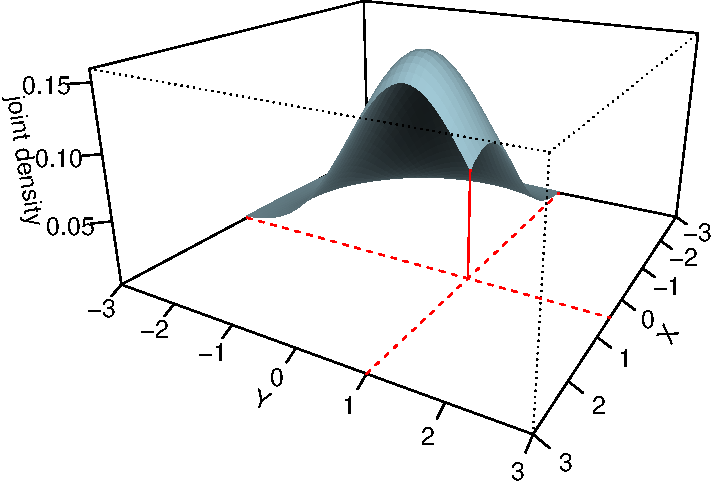
\includegraphics[width=0.95\linewidth]{EcoStat_files/figure-latex/essai3d2-1} \caption{The volume between the horizontal plane ($z=0$) and the surface is equal to $F_{XY}(0.5,1)=\mathbb{P}(X<0.5,Y<1)$.}\label{fig:essai3d2}
\end{figure}

\begin{definition}[Joint probability density function (p.d.f.)]
\protect\hypertarget{def:jointpdf}{}\label{def:jointpdf}The continuous random variables \(X\) and \(Y\) admit the joint p.d.f. \(f_{XY}\), where \(f_{XY}(x,y) \ge 0\) for all \(x\) and \(y\), if:
\[
\mathbb{P}(a < X \le b,c < Y \le d) = \int_{a}^{b}\int_{c}^{d}f_{XY}(x,y)dx dy, \quad \forall a \le b,\;c \le d.
\]
\end{definition}

In particular, we have:
\begin{eqnarray*}
&&f_{XY}(x,y)\\
&=& \lim_{\varepsilon \rightarrow 0} \frac{\mathbb{P}(x < X \le x + \varepsilon,y < Y \le y + \varepsilon)}{\varepsilon^2} \\
&=& \lim_{\varepsilon \rightarrow 0} \frac{F_{XY}(x + \varepsilon,y + \varepsilon)-F_{XY}(x,y + \varepsilon)-F_{XY}(x + \varepsilon,y)+F_{XY}(x,y)}{\varepsilon^2}.
\end{eqnarray*}

\begin{figure}
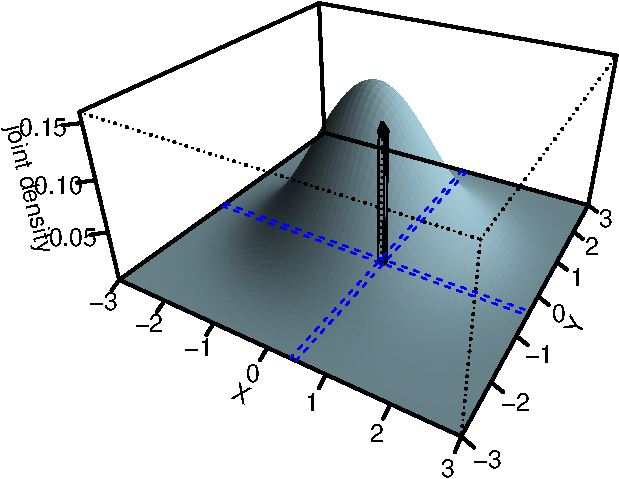
\includegraphics[width=0.95\linewidth]{EcoStat_files/figure-latex/essai3d-1} \caption{Assume that the basis of the black column is defined by those points whose $x$-coordinates are between $x$ and $x+\varepsilon$ and $y$-coordinates are between $y$ and $y+\varepsilon$. Then the volume of the black column is equal to $\mathbb{P}(x < X \le x+\varepsilon,y < Y \le y+\varepsilon)$, which is approximately equal to $f_{XY}(x,y)\varepsilon^2$ if $\varepsilon$ is small.}\label{fig:essai3d}
\end{figure}

\begin{definition}[Conditional probability distribution function]
\protect\hypertarget{def:condcdf}{}\label{def:condcdf}If \(X\) and \(Y\) are continuous r.v., then the distribution of \(X\) conditional on \(Y=y\), which we denote by \(f_{X|Y}(x,y)\), satisfies:
\[
f_{X|Y}(x,y)=\lim_{\varepsilon \rightarrow 0} \frac{\mathbb{P}(x < X \le x + \varepsilon|Y=y)}{\varepsilon}.
\]
\end{definition}

\begin{proposition}[Conditional probability distribution function]
\protect\hypertarget{prp:condcdf}{}\label{prp:condcdf}We have
\[
f_{X|Y}(x,y)=\frac{f_{XY}(x,y)}{f_Y(y)}.
\]
\end{proposition}

\begin{proof}
We have:
\begin{eqnarray*}
f_{X|Y}(x,y)&=&\lim_{\varepsilon \rightarrow 0} \frac{\mathbb{P}(x < X \le x + \varepsilon|Y=y)}{\varepsilon}\\
&=&\lim_{\varepsilon \rightarrow 0} \frac{1}{\varepsilon}\mathbb{P}(x < X \le x + \varepsilon|y<Y\le y+\varepsilon)\\
&=&\lim_{\varepsilon \rightarrow 0} \frac{1}{\varepsilon}\frac{\mathbb{P}(x < X \le x + \varepsilon,y<Y\le y+\varepsilon)}{\mathbb{P}(y<Y\le y+\varepsilon)}\\
&=&\lim_{\varepsilon \rightarrow 0} \frac{1}{\varepsilon} \frac{\varepsilon^2f_{XY}(x,y)}{\varepsilon f_{Y}(y)}.
\end{eqnarray*}
\end{proof}

\begin{definition}[Independent random variables]
\protect\hypertarget{def:independent}{}\label{def:independent}Consider two r.v., \(X\) and \(Y\), with respective c.d.f. \(F_X\) and \(F_Y\), and respective p.d.f. \(f_X\) and \(f_Y\).

These random variables are independent if and only if (iff) the joint c.d.f. of \(X\) and \(Y\) (see Def. \ref{def:jointcdf}) is given by:
\[
F_{XY}(x,y) = F_{X}(x) \times F_{Y}(y),
\]
or, equivalently, iff the joint p.d.f. of \((X,Y)\) (see Def. \ref{def:jointpdf}) is given by:
\[
f_{XY}(x,y) = f_{X}(x) \times f_{Y}(y).
\]
\end{definition}

We have the following:

\begin{enumerate}
\def\labelenumi{\arabic{enumi}.}
\tightlist
\item
  If \(X\) and \(Y\) are independent, \(f_{X|Y}(x,y)=f_{X}(x)\). This implies, in particular, that \(\mathbb{E}(g(X)|Y)=\mathbb{E}(g(X))\), where \(g\) is any function.
\item
  If \(X\) and \(Y\) are independent, then \(\mathbb{E}(g(X)h(Y))=\mathbb{E}(g(X))\mathbb{E}(h(Y))\) and \(\mathbb{C}ov(g(X),h(Y))=0\), where \(g\) and \(h\) are any functions.
\end{enumerate}

It is important to note that the absence of correlation between two variables is not a sufficient condition to have independence. Consider for instance the case where \(X=Y^2\), with \(Y \sim\mathcal{N}(0,1)\). In this case, we have \(\mathbb{C}ov(X,Y)=0\), but \(X\) and \(Y\) are not independent. Indeed, we have for instance \(\mathbb{E}(Y^2 \times X)=3\), which is not equal to \(\mathbb{E}(Y^2) \times \mathbb{E}(X)=1\). (If \(X\) and \(Y\) were independent, we should have \(\mathbb{E}(Y^2 \times X)=\mathbb{E}(Y^2) \times \mathbb{E}(X)\) according to point 2 above.)

\hypertarget{law-of-iterated-expectations}{%
\section{Law of iterated expectations}\label{law-of-iterated-expectations}}

\begin{proposition}[Law of iterated expectations]
\protect\hypertarget{prp:lawiteratedexpect}{}\label{prp:lawiteratedexpect}If \(X\) and \(Y\) are two random variables and if \(\mathbb{E}(|X|)<\infty\), we have:
\[
\boxed{\mathbb{E}(X) = \mathbb{E}(\mathbb{E}(X|Y)).}
\]
\end{proposition}

\begin{proof}
(in the case where the p.d.f. of \((X,Y)\) exists) Let us denote by \(f_X\), \(f_Y\) and \(f_{XY}\) the probability distribution functions (p.d.f.) of \(X\), \(Y\) and \((X,Y)\), respectively. We have:
\[
f_{X}(x) = \int f_{XY}(x,y) dy.
\]
Besides, we have (Bayes equality, Prop. \ref{prp:condcdf}):
\[
f_{XY}(x,y) = f_{X|Y}(x,y)f_{Y}(y).
\]
Therefore:
\begin{eqnarray*}
\mathbb{E}(X) &=& \int x f_X(x)dx = \int x  \underbrace{ \int  f_{XY}(x,y) dy}_{=f_X(x)} dx =\int  \int x f_{X|Y}(x,y)f_{Y}(y) dydx \\
& = & \int \underbrace{\left(\int x f_{X|Y}(x,y)dx\right)}_{\mathbb{E}[X|Y=y]}f_{Y}(y) dy = \mathbb{E} \left( \mathbb{E}[X|Y] \right).
\end{eqnarray*}
\end{proof}

\begin{example}[Mixture of Gaussian distributions]
\protect\hypertarget{exm:mixture}{}\label{exm:mixture}By definition, \(X\) is drawn from a mixture of Gaussian distributions if:
\[
X = \color{blue}{B \times Y_1} + \color{red}{(1-B) \times Y_2},
\]
where \(B\), \(Y_1\) and \(Y_2\) are three independent variables drawn as follows:
\[
B \sim \mbox{Bernoulli}(p),\quad Y_1 \sim \mathcal{N}(\mu_1,\sigma_1^2), \quad \mbox{and}\quad Y_2 \sim \mathcal{N}(\mu_2,\sigma_2^2).
\]

Figure \ref{fig:mixtureG} displays the pdfs associated with three different mixtures of Gaussian distributions. (This \href{https://jrenne.shinyapps.io/density/}{web-interface} allows to produce the pdf associated for any other parameterization.)

\begin{figure}
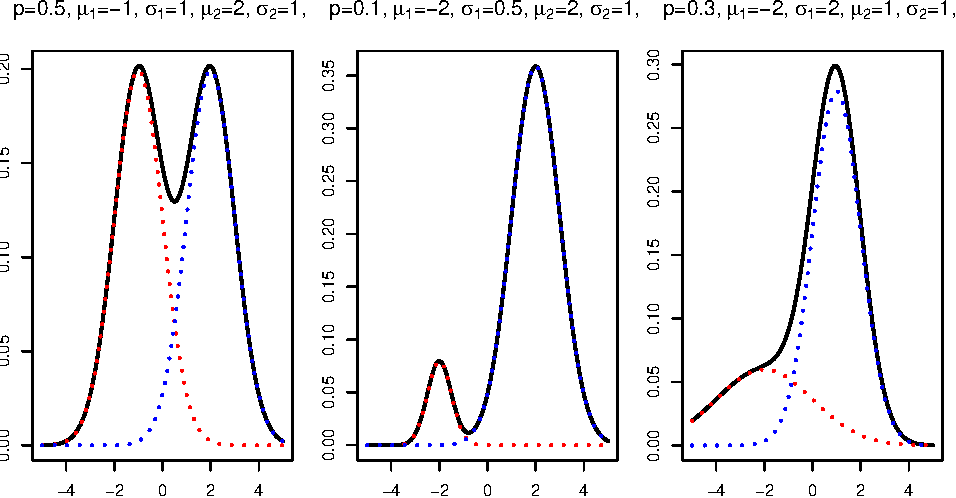
\includegraphics[width=0.95\linewidth]{EcoStat_files/figure-latex/mixtureG-1} \caption{Example of pdfs of mixtures of Gaussian distribututions.}\label{fig:mixtureG}
\end{figure}

The law of iterated expectations gives:
\[
\mathbb{E}(X) = \mathbb{E}(\mathbb{E}(X|B)) = \mathbb{E}(B\mu_1+(1-B)\mu_2)=p\mu_1 + (1-p)\mu_2.
\]
\end{example}

\begin{example}[Buffon (1733)'s needles]
\protect\hypertarget{exm:Buffon}{}\label{exm:Buffon}Suppose we have a floor made of parallel strips of wood, each the same width {[}\(w=1\){]}. We drop a needle, of length \(1/2\), onto the floor. What is the probability that the needle crosses the grooves of the floor?

Let's define the random variable \(X\) by
\[
X = \left\{
\begin{array}{cl}
1 & \mbox{if the needle crosses a line}\\
0 & \mbox{otherwise.}
\end{array}
\right.
\]
Conditionally on \(\theta\), it can be seen that we have \(\mathbb{E}(X|\theta)=\cos(\theta)/2\) (see Figure \ref{fig:Buffon}).

\begin{figure}
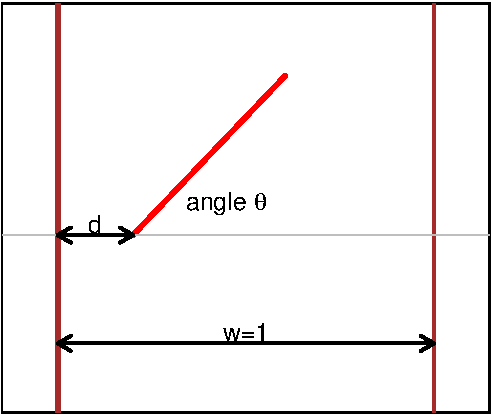
\includegraphics[width=0.95\linewidth]{EcoStat_files/figure-latex/Buffon-1} \caption{Schematic representation of the problem.}\label{fig:Buffon}
\end{figure}

It is reasonable to assume that \(\theta\) is uniformly distributed on \([-\pi/2,\pi/2]\), therefore:
\[
\mathbb{E}(X)=\mathbb{E}(\mathbb{E}(X|\theta))=\mathbb{E}(\cos(\theta)/2)=\int_{-\pi/2}^{\pi/2}\frac{1}{2}\cos(\theta)\left(\frac{d\theta}{\pi}\right)=\frac{1}{\pi}.
\]

{[}This \href{https://jrenne.shinyapps.io/StatEcoII/}{web-interface} allows to simulate the present experiment (select Worksheet ``Buffon's needles'').{]}
\end{example}

\hypertarget{law-of-total-variance}{%
\section{Law of total variance}\label{law-of-total-variance}}

\begin{proposition}[Law of total variance]
\protect\hypertarget{prp:lawtotalvariance}{}\label{prp:lawtotalvariance}If \(X\) and \(Y\) are two random variables and if the variance of \(X\) is finite, we have:
\[
\boxed{\mathbb{V}ar(X) = \mathbb{E}(\mathbb{V}ar(X|Y)) + \mathbb{V}ar(\mathbb{E}(X|Y)).}
\]
\end{proposition}

\begin{proof}
We have:
\begin{eqnarray*}
\mathbb{V}ar(X) &=& \mathbb{E}(X^2) - \mathbb{E}(X)^2\\
&=& \mathbb{E}(\mathbb{E}(X^2|Y)) - \mathbb{E}(X)^2\\
&=& \mathbb{E}(\mathbb{E}(X^2|Y) \color{blue}{- \mathbb{E}(X|Y)^2}) +  \color{blue}{\mathbb{E}(\mathbb{E}(X|Y)^2)}  - \color{red}{\mathbb{E}(X)^2}\\
&=& \mathbb{E}(\underbrace{\mathbb{E}(X^2|Y) - \mathbb{E}(X|Y)^2}_{\mathbb{V}ar(X|Y)}) + \underbrace{\mathbb{E}(\mathbb{E}(X|Y)^2) - \color{red}{\mathbb{E}(\mathbb{E}(X|Y))^2}}_{\mathbb{V}ar(\mathbb{E}(X|Y))}.
\end{eqnarray*}
\end{proof}

\begin{example}[Mixture of Gaussian distributions (cont'd)]
\protect\hypertarget{exm:mixture2}{}\label{exm:mixture2}Consider the case of a mixture of Gaussian distributions (Example \ref{exm:mixture}). We have:
\begin{eqnarray*}
\mathbb{V}ar(X) &=& \color{blue}{\mathbb{E}(\mathbb{V}ar(X|B))} + \color{red}{\mathbb{V}ar(\mathbb{E}(X|B))}\\
&=&  \color{blue}{p\sigma_1^2+(1-p)\sigma_2^2} + \color{red}{p(1-p)(\mu_1 - \mu_2)^2}.
\end{eqnarray*}
\end{example}

\hypertarget{about-consistent-estimators}{%
\section{About consistent estimators}\label{about-consistent-estimators}}

The objective of econometrics is to estimate parameters out of data observations (samples). Examples of parameters of interest include, among many others: causal effect of a variable on another, elasticities, parameters defining some distribution of interest, preference parameters (risk aversion)\ldots{}

Except in degenerate cases, the estimates are different from the ``true'' (or \emph{population}) value. A good estimator is expected to converge to the true value when the sample size increases. That is, we are interested in the \emph{consistency} of the estimator.

Denote by \(\hat\theta_n\) the estimate of \(\theta\) based on a sample of length \(n\). We say that \(\hat\theta\) is a consistent estimator of \(\theta\) if, for any \(\varepsilon>0\) (even if very small), the probability that \(\hat\theta_n\) is in \([\theta - \varepsilon,\theta + \varepsilon]\) goes to 1 when \(n\) goes to \(\infty\). Formally:
\[
\lim_{n \rightarrow + \infty} \mathbb{P}\left(\hat\theta_n \in [\theta - \varepsilon,\theta + \varepsilon]\right) = 1.
\]

That is, \(\hat\theta\) is a consistent estimator if \(\hat\theta_n\) \emph{converges in probability} (Def. \ref{def:convergenceproba}) to \(\theta\). Note that there exist different types of stochastic convergence.\footnote{Appendix \ref{StochConvergences} notably provides the definitions of the convergence in distribution (Def. \ref{def:cvgceDistri}) and the mean-square convergence (Def. \ref{def:convergenceLr}).}

\begin{example}[Example of non-convergent estimator]
\protect\hypertarget{exm:NonConsist}{}\label{exm:NonConsist}

Assume that \(X_i \sim i.i.d. \mbox{Cauchy}\) with a location parameter of 1 and a scale parameter of 1 (Def. \ref{def:Cauchy}). The sample mean \(\bar{X}_n = \frac{1}{n}\sum_{i=1}^{n} X_i\) does not converge in probability. This is because a Cauchy distribution has no mean; hence the law of large numbers (Theorem \ref{thm:LLN}) does not apply.

\begin{figure}
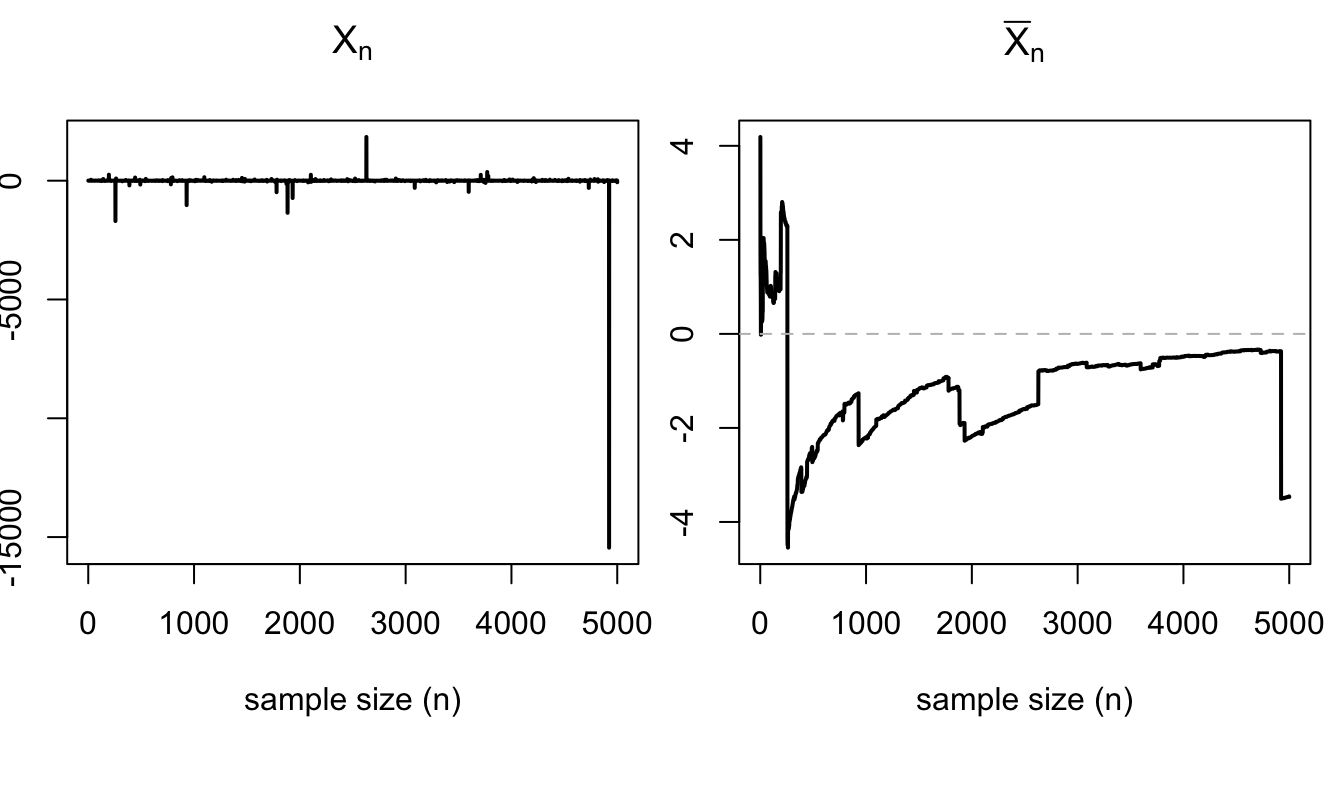
\includegraphics[width=0.95\linewidth]{EcoStat_files/figure-latex/figCauchy-1} \caption{Simulation of $\bar{X}_n$ when $X_i \sim i.i.d. \mbox{Cauchy}$.}\label{fig:figCauchy}
\end{figure}

\end{example}

\hypertarget{TCL}{%
\chapter{Central Limit Theorem}\label{TCL}}

The law of large numbers (LLN) and the central limit theorem (CLT) are two fundamental theorems of probability. The former states that the sample mean converges in probability to the population mean (when it exists). The latter states that the distribution of the sum (or average) of a large number of independent, identically distributed (i.i.d.) variables with finite variance is approximately normal, regardless of the underlying distribution (as long as it features a finite variance).

\hypertarget{law-of-large-numbers}{%
\section{Law of large numbers}\label{law-of-large-numbers}}

\begin{definition}[Sample and Population]
\protect\hypertarget{def:smplpop}{}\label{def:smplpop}In statistics, a \emph{sample} refers to a finite set of observations drawn from a \emph{population}.
\end{definition}

Most of the time, it is necessary to use samples for research, because it is impractical to study the whole population. Typically, it is rare to observe the population mean, and we often use instead sample means (or averages). The sample average of \(\{x_1,\dots,x_n\}\) is given by:
\[
\overline{x}_n = \frac{1}{n}\sum_{i=1}^n x_i.
\]
This sample mean is an estimator of the true (population) mean \(\mathbb{E}(x_i)\) (assuming the latter exists). According to the law of large numbers (Theorem \ref{thm:LLN}), this estimator is \emph{consistent}. (see Def. \ref{def:convergenceproba} for the definition of convergence in probability.)

\begin{theorem}[Law of large numbers]
\protect\hypertarget{thm:LLN}{}\label{thm:LLN}The sample mean is a consistent estimator of the population mean. In other words, the sample mean converges in probability to the population mean.
\end{theorem}

\begin{proof}
See Appendix \ref{CLTappend}.
\end{proof}

\begin{example}
\protect\hypertarget{exm:doctorVisits}{}\label{exm:doctorVisits}

Suppose one is interested in the average number of doctor consultations over 12 months, for Swiss people. One can get an estimate by computing the sample average of a large dataset, for instance using the \href{https://forscenter.ch/projects/swiss-household-panel/}{Swiss Household Panel (SHP)}:

Figure \ref{fig:incomeDistri} shows the empirical distribution of the number of doctor visits.

\begin{Shaded}
\begin{Highlighting}[]
\FunctionTok{library}\NormalTok{(AEC) }\CommentTok{\# to load the shp data{-}frame.}
\NormalTok{Nb.doct.visits }\OtherTok{\textless{}{-}}\NormalTok{ shp}\SpecialCharTok{$}\NormalTok{p19c15}
\NormalTok{Nb.doct.visits }\OtherTok{\textless{}{-}}\NormalTok{ Nb.doct.visits[Nb.doct.visits}\SpecialCharTok{\textgreater{}=}\DecValTok{0}\NormalTok{] }\CommentTok{\# remove irrelevant observations}
\FunctionTok{par}\NormalTok{(}\AttributeTok{plt=}\FunctionTok{c}\NormalTok{(.}\DecValTok{15}\NormalTok{,.}\DecValTok{95}\NormalTok{,.}\DecValTok{2}\NormalTok{,.}\DecValTok{95}\NormalTok{))}
\FunctionTok{barplot}\NormalTok{(}\FunctionTok{table}\NormalTok{(Nb.doct.visits),}\AttributeTok{xlim=}\FunctionTok{c}\NormalTok{(}\DecValTok{0}\NormalTok{,}\DecValTok{25}\NormalTok{))}
\end{Highlighting}
\end{Shaded}

\begin{figure}
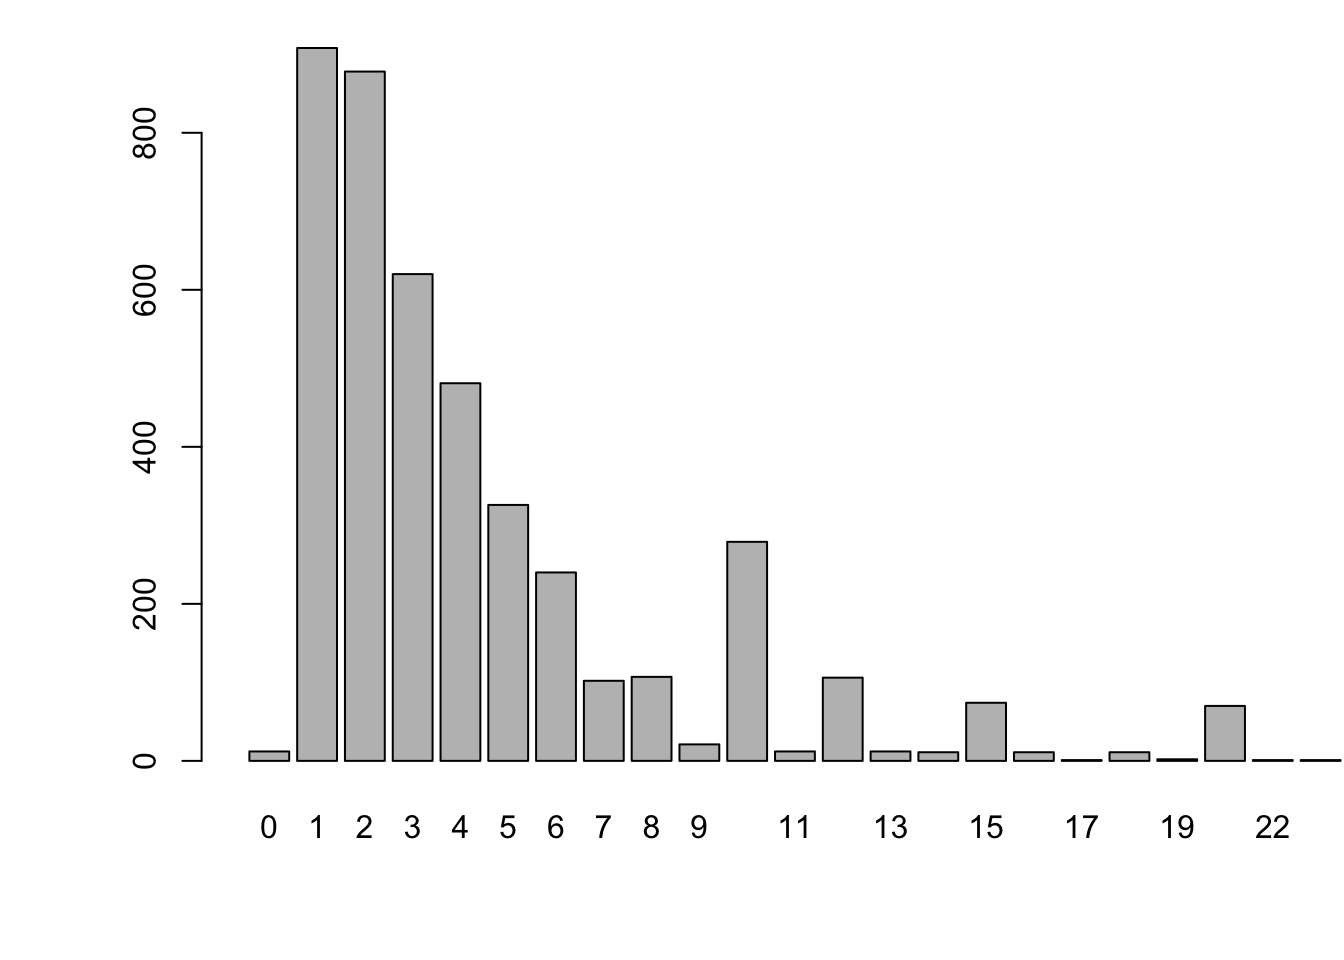
\includegraphics{EcoStat_files/figure-latex/incomeDistri-1} \caption{Distribution of the number of doctor visits. Source: Swiss Household Panel.}\label{fig:incomeDistri}
\end{figure}

\begin{Shaded}
\begin{Highlighting}[]
\FunctionTok{cbind}\NormalTok{(}\FunctionTok{mean}\NormalTok{(Nb.doct.visits),}\FunctionTok{var}\NormalTok{(Nb.doct.visits))}
\end{Highlighting}
\end{Shaded}

\begin{verbatim}
##          [,1]     [,2]
## [1,] 5.253816 79.50575
\end{verbatim}

Let us compute the sample mean and variance:

\begin{Shaded}
\begin{Highlighting}[]
\FunctionTok{cbind}\NormalTok{(}\FunctionTok{mean}\NormalTok{(Nb.doct.visits),}\FunctionTok{var}\NormalTok{(Nb.doct.visits))}
\end{Highlighting}
\end{Shaded}

\begin{verbatim}
##          [,1]     [,2]
## [1,] 5.253816 79.50575
\end{verbatim}

\end{example}

How to know whether the sample mean is a good estimate of the true (population) average? In other words, how to measure the accuracy of the estimator?

A first answer is provided by the Chebychev inequality. Assume the \(x_i\)'s are independently drawn from a distribution of mean \(\mu\) and variance \(\sigma^2\). We have:
\[
\mathbb{E}(\bar{x}_n) = \mu \quad \mbox{ and } \quad \mathbb{V}ar(\mu - \bar{x}_n) = \frac{1}{n}\sigma^2 \underset{n \rightarrow \infty}{\rightarrow} 0.
\]
The Chebychev inequality (Proposition \ref{prp:chebychev}) states that, for any \(\varepsilon > 0\) (even very small), we have:
\[
\mathbb{P}(|\bar{x}_n-\mu|>\varepsilon) \le \frac{\mathbb{V}ar(\mu - \bar{x}_n)}{\varepsilon^2} = \frac{\sigma^2}{n\varepsilon^2} \underset{n \rightarrow \infty}{\rightarrow} 0.
\]
Consider for instance the estimation of the average number of doctor visits (Example \ref{exm:doctorVisits}). In this example, the sample length is \(n=\) 4389, we have \(\bar{x}_n=\) 5.25, and the variance \(\sigma^2\) was approximately equal to 79.51. Therefore, taking \(\varepsilon=0.5\), we have that \(\mathbb{P}(\bar{x}_n-0.5<\mu<\bar{x}_n+0.5)\) is lower than \(\frac{\sigma^2}{n\varepsilon^2} \approx\)
0.072.

However, this only gives bounds for such probabilities. The central limit theorem provides richer information, as it gives the approximate distribution of the estimation error.

\hypertarget{central-limit-theorem-clt}{%
\section{Central Limit Theorem (CLT)}\label{central-limit-theorem-clt}}

\begin{theorem}[Lindberg-Levy Central limit theorem, CLT]
\protect\hypertarget{thm:LindbergLevyCLT}{}\label{thm:LindbergLevyCLT}If \(x_n\) is an i.i.d. sequence of random variables with mean \(\mu\) and (finite) variance, then:
\[
\boxed{\sqrt{n} (\bar{x}_n - \mu) \overset{d}{\rightarrow} \mathcal{N}(0,\sigma^2), \quad \mbox{where} \quad \bar{x}_n = \frac{1}{n} \sum_{i=1}^{n} x_i.}
\]
{[}``\(\overset{d}{\rightarrow}\)'' denotes the convergence in distribution (see Def. \ref{def:cvgceDistri}){]}
\end{theorem}

\begin{proof}
See Appendix \ref{CLTappend}.
\end{proof}

According to the CLT, when \(n\) is large and whatever the distribution of the \(x_i\)'s (as long as it features an average \(\mu\) and a variance \(\sigma^2\)), the error between \(\bar{x}_n\) and \(\mu\) can be seen as a random variable that is normally distributed; it is of mean zero and its standard deviation is \(\sigma/\sqrt{n}\). (We then say that the convergence rate is \emph{in \(\sqrt{n}\)}.) The knowledge of the quantiles of the normal distribution can then be used to compute approximate confidence intervals for \(\mu\) (based on the sample \(\{x_1,\dots,x_n\}\)).

This \href{https://jrenne.shinyapps.io/StatEcoII/}{web interface} illustrates the CLT with simulations (select the ``CLT'' block).

The CL theorem was first postulated by the mathematician Abraham de Moivre. In an article published in 1733, he used the normal distribution to approximate the distribution of the number of heads resulting from many tosses of a fair coin. This finding was nearly forgotten until Pierre-Simon Laplace recalled it in his\href{https://archive.org/details/thorieanalytiqu01laplgoog}{Théorie analytique des probabilités}, published in 1812. Laplace expanded De Moivre's finding by approximating the binomial distribution with the normal distribution.

\begin{exercise}
\protect\hypertarget{exr:ExoBuffon}{}\label{exr:ExoBuffon}Consider Buffon's experiment (Example \ref{exm:Buffon}). We have seen that \(\pi\) can be estimated by counting the fraction of times the needles cross the grooves of the floor.\footnote{More precisely, the expectation of this fraction is equal to \(1/\pi\).} Using the CLT, determine the (approximate) minimal number \(n\) of needles that one has to throw to get an estimate \(\hat\pi\) (\(= 1/\bar{X}_n\)) of \(\pi\) that is such that there is a 95\% chance that \(\pi \in [\hat\pi-0.01,\hat\pi+0.01]\)?
\end{exercise}

\begin{exercise}
\protect\hypertarget{exr:ExoPileFace}{}\label{exr:ExoPileFace}Assume you have a lot of time and a coin. How would you approximate the 100 percentiles of the \(\mathcal{N}(0,1)\) distribution?
\end{exercise}

The CLT can be extended to the case where each \(x_i\) is a vector. (In that case, and if the dimension of \(x_i\) is \(m\), then \(\mathbb{V}ar(x_i)\) is a \(m\times m\) matrix.) Here is the multivariate CLT:

\begin{theorem}[Multivariate Central limit theorem, CLT]
\protect\hypertarget{thm:MCLT}{}\label{thm:MCLT}If \(\mathbf{x}_n\) is an i.i.d. sequence of \(m\)-dimensional random variables with mean \(\boldsymbol\mu\) and variance \(\Sigma\), where \(\Sigma\) is a positive definite matrix, then:
\[
\boxed{\sqrt{n} (\bar{\mathbf{x}}_n - \boldsymbol\mu) \overset{d}{\rightarrow} \mathcal{N}(\mathbf{0},\Sigma), \quad \mbox{where} \quad \bar{\mathbf{x}}_n = \frac{1}{n} \sum_{i=1}^{n} \mathbf{x}_i.}
\]
\end{theorem}

\hypertarget{comparison-of-sample-means}{%
\section{Comparison of sample means}\label{comparison-of-sample-means}}

As said at the beginning of this chapter, the CLT is a key statistical result that has numerous applications. An important one is the statistical comparision of sample means:

Consider two samples \(\{m_1,\dots,m_{n_m}\}\) and \(\{w_1,\dots,w_{n_w}\}\). Assume that the \(m_i\)'s (respectively the \(w_i\)'s) are i.i.d., with mean \(\mu_m\) and variance \(\sigma^2_m\) and of \(w_i\)'s (resp. with mean \(\mu_w\) and variance \(\sigma^2_w\)).

If \(n\) is large, according to the CLT, we approximately have:
\[
\sqrt{n_m}(\bar{m} - \mu_m) \sim \mathcal{N}(0,\sigma^2_m) \quad and \quad \sqrt{n_w}(\bar{w} - \mu_w) \sim \mathcal{N}(0,\sigma^2_w),
\]
or
\[
\bar{m} \sim \mathcal{N}\left(\mu_m,\frac{\sigma^2_m}{n_m}\right) \quad and \quad \bar{w} \sim \mathcal{N}\left(\mu_w,\frac{\sigma^2_w}{n_w}\right).
\]

if the \(m_i\)'s and the \(w_i\)'s are independent, then \(\bar{m}\) and \(\bar{w}\) also are, and we get:
\[
\bar{m} - \bar{w} \sim \mathcal{N}\left(\mu_m-\mu_w,\sigma^2\right) \quad with \quad \sigma^2 = \frac{\sigma^2_m}{n_m}+\frac{\sigma^2_w}{n_w}.
\]
This can be used to test the null hypothesis \(H_0: \; \mu_m-\mu_w = 0\) (see Section \ref{Tests}). Indeed under this assumption, the probability that \(\bar{m} - \bar{w}\) is in \([-1.96\sigma,1.96\sigma]\) (respectively in \([-2.58\sigma,2.58\sigma]\)) is approximately 0.95 (respectively 0.99) {[}see Table \ref{tab:Normal}{]}.

For instance, if we find, using our sample, that \(\bar{m} - \bar{w}\) is not in \([-2.58\sigma,2.58\sigma]\), then we reject the null hypothesis at the 1\% significance level.

\begin{example}[Comparison of sample means]
\protect\hypertarget{exm:comparSmplMeans}{}\label{exm:comparSmplMeans}Let us use the \href{https://forscenter.ch/projects/swiss-household-panel/}{Swiss Household Panel (SHP)} dataset to test the equality between men and women incomes, for Swiss people under the age of 35.

The next lines of codes construct two samples of incomes; one for men (\texttt{income.m}), and one for women (\texttt{income.w}).

\begin{Shaded}
\begin{Highlighting}[]
\FunctionTok{library}\NormalTok{(AEC);}\FunctionTok{library}\NormalTok{(logKDE)}
\NormalTok{dataset.m }\OtherTok{\textless{}{-}} \FunctionTok{subset}\NormalTok{(shp,(sex19}\SpecialCharTok{==}\DecValTok{1}\NormalTok{)}\SpecialCharTok{\&}\NormalTok{(age19}\SpecialCharTok{\textless{}=}\DecValTok{35}\NormalTok{))}
\NormalTok{dataset.w }\OtherTok{\textless{}{-}} \FunctionTok{subset}\NormalTok{(shp,(sex19}\SpecialCharTok{==}\DecValTok{2}\NormalTok{)}\SpecialCharTok{\&}\NormalTok{(age19}\SpecialCharTok{\textless{}=}\DecValTok{35}\NormalTok{))}
\NormalTok{income.m }\OtherTok{\textless{}{-}}\NormalTok{ dataset.m}\SpecialCharTok{$}\NormalTok{i19ptotg}
\NormalTok{income.w }\OtherTok{\textless{}{-}}\NormalTok{ dataset.w}\SpecialCharTok{$}\NormalTok{i19ptotg}
\NormalTok{income.m }\OtherTok{\textless{}{-}}\NormalTok{ income.m[income.m}\SpecialCharTok{\textgreater{}=}\DecValTok{0}\NormalTok{] }\CommentTok{\# remove irrelevant data}
\NormalTok{income.w }\OtherTok{\textless{}{-}}\NormalTok{ income.w[income.w}\SpecialCharTok{\textgreater{}=}\DecValTok{0}\NormalTok{] }\CommentTok{\# remove irrelevant data}
\end{Highlighting}
\end{Shaded}

Figure \ref{fig:RcompMeans} displays the empirical densities of incomes for men and women. Vertical dashed lines indicate sample means:

\begin{Shaded}
\begin{Highlighting}[]
\FunctionTok{par}\NormalTok{(}\AttributeTok{plt=}\FunctionTok{c}\NormalTok{(.}\DecValTok{1}\NormalTok{,.}\DecValTok{95}\NormalTok{,.}\DecValTok{2}\NormalTok{,.}\DecValTok{95}\NormalTok{)) }\CommentTok{\# adjust margins}
\FunctionTok{plot}\NormalTok{(}\FunctionTok{logdensity}\NormalTok{(income.w),}\AttributeTok{lwd=}\DecValTok{2}\NormalTok{,}\AttributeTok{xlim=}\FunctionTok{c}\NormalTok{(}\DecValTok{0}\NormalTok{,}\DecValTok{200000}\NormalTok{),}\AttributeTok{main=}\StringTok{""}\NormalTok{,}
     \AttributeTok{xlab=}\StringTok{"Yearly gross income (in CHF)"}\NormalTok{,}\AttributeTok{ylab=}\StringTok{""}\NormalTok{) }\CommentTok{\# x and y labels}
\FunctionTok{lines}\NormalTok{(}\FunctionTok{logdensity}\NormalTok{(income.m),}\AttributeTok{col=}\StringTok{"red"}\NormalTok{,}\AttributeTok{lwd=}\DecValTok{2}\NormalTok{)}
\FunctionTok{abline}\NormalTok{(}\AttributeTok{v=}\FunctionTok{mean}\NormalTok{(income.m),}\AttributeTok{col=}\StringTok{"red"}\NormalTok{,}\AttributeTok{lty=}\DecValTok{3}\NormalTok{,}\AttributeTok{lwd=}\DecValTok{2}\NormalTok{)}
\FunctionTok{abline}\NormalTok{(}\AttributeTok{v=}\FunctionTok{mean}\NormalTok{(income.w),}\AttributeTok{col=}\StringTok{"black"}\NormalTok{,}\AttributeTok{lty=}\DecValTok{3}\NormalTok{,}\AttributeTok{lwd=}\DecValTok{2}\NormalTok{)}
\FunctionTok{legend}\NormalTok{(}\StringTok{"topright"}\NormalTok{,}\FunctionTok{c}\NormalTok{(}\StringTok{"men yearly income"}\NormalTok{,}\StringTok{"women"}\NormalTok{),}\AttributeTok{lty=}\DecValTok{1}\NormalTok{,}\AttributeTok{lwd=}\DecValTok{2}\NormalTok{,}\AttributeTok{col=}\FunctionTok{c}\NormalTok{(}\StringTok{"red"}\NormalTok{,}\StringTok{"black"}\NormalTok{))}
\end{Highlighting}
\end{Shaded}

\begin{figure}
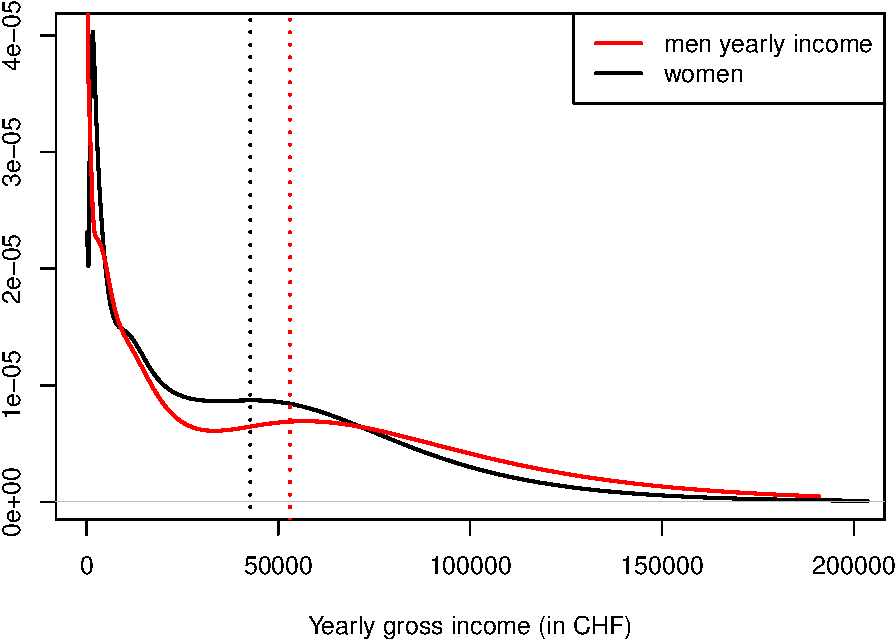
\includegraphics{EcoStat_files/figure-latex/RcompMeans-1} \caption{Distribution of yearly gross incomes for Swiss residents under the age of 35. Source: SHP. Vertical dashed lines indicates the sample mean.}\label{fig:RcompMeans}
\end{figure}

Let us compute \(\bar{m}\), \(\bar{w}\), and \(\sigma\):

\begin{Shaded}
\begin{Highlighting}[]
\NormalTok{m.bar }\OtherTok{\textless{}{-}} \FunctionTok{mean}\NormalTok{(income.m)}
\NormalTok{w.bar }\OtherTok{\textless{}{-}} \FunctionTok{mean}\NormalTok{(income.w)}
\NormalTok{sigma }\OtherTok{\textless{}{-}} \FunctionTok{sqrt}\NormalTok{(}\FunctionTok{var}\NormalTok{(income.m)}\SpecialCharTok{/}\FunctionTok{length}\NormalTok{(income.m) }\SpecialCharTok{+} \FunctionTok{var}\NormalTok{(income.w)}\SpecialCharTok{/}\FunctionTok{length}\NormalTok{(income.w))}
\FunctionTok{print}\NormalTok{(}\FunctionTok{c}\NormalTok{(m.bar,w.bar,sigma))}
\end{Highlighting}
\end{Shaded}

\begin{verbatim}
## [1] 53035.023 42708.227  2427.425
\end{verbatim}

Under the ``equality assumption'', their would a probability of only 5\% (respectively 1\%) for \(\bar{m} - \bar{w}\) not to be in \([\)-4758,4758\(]\) (respectively in \([\)-6263,6263\(]\)). Since \(\bar{m} - \bar{w}\) is equal to 10327, we reject the null hypothesis at the 5\%, and even 1\%, significance levels.
\end{example}

\hypertarget{Tests}{%
\chapter{Statistical tests}\label{Tests}}

We run a statistical test when we want to know whether some hypothesis about a vector of parameters \(\theta\) ---that is imperfectly observed--- is consistent with data that are seen as random, and whose randomness depend on \(\theta\).

Typically, assume you observe a sample \(\mathbf{x}=\{x_1,\dots,x_n\}\) where the \(x_i\)'s are i.i.d., of mean \(\mu\) and variance \(\sigma^2\) (these two parameters being unobseved). One may want to know whether \(\mu=0\) or, maybe, whether \(\sigma = 1\).

The hypothesis the researcher wants to test is called the \emph{null hypothesis}. It is often denoted by \(H_0\). It is a conjecture about a given property of a population. Without loss of generality, it can be stated as:
\[
H_0:\;\{\theta \in \Theta\}.
\]
It can also be defined through a function \(h\) (say):\footnote{We can relate the previous and the next equation through \(\Theta = \{\theta, \,s.t.\,h(\theta)=0\}\).}
\[
H_0:\;h(\theta)=0.
\]

The \emph{alternative hypothesis}, often denoted \(H_1\) is then defined by \(H_1:\;\{\theta \in \Theta^c\}\).\footnote{Note that researchers may want to find support for the null hypothesis \(H_0\) as well as for the alternative hypothesis \(H_1\).}

The ingredients of a statistical test are:

\begin{itemize}
\tightlist
\item
  a vector of (unknown) parameters (\(\theta\)),
\item
  a \textbf{test statistic}, that is a function of the sample components (\(S(\mathbf{x})\), say), and
\item
  a \textbf{critical region} (\(\Omega\), say), defined as a set of implausible values of \(S\) under \(H_0\).
\end{itemize}

To implement a test statistic, we need to know the distribution of \(S\) under the null hypothesis \(H_0\). Equipped, with such a distribution, we compute \(S(\mathbf{x})\) and we look at its location; more specifically, we look whether it lies within the critical region \(\Omega\). The latter corresponds to ``implausible'' regions of this distribution (typically the tails). If \(S \in \Omega\), then we reject the null hypothesis. Looselly speaking; it amounts to saying: \emph{if \(H_0\) were true, it would have been unlikely to get such a large (or small) draw for \(S\)}.

Hence, there are two possible outcomes for a statisitcal test:

\begin{itemize}
\tightlist
\item
  \(H_0\) is rejected if \(S \in \Omega\);
\item
  \(H_0\) is not rejected if \(S \not\in \Omega\).
\end{itemize}

Except in extreme cases, there is always a non-zero probability to reject \(H_0\) while it is true (\textbf{Type I error}, or \textbf{false positive}), or to fail to reject it while it is false (\textbf{Type II error}, or \textbf{false negative}).

This vocabulary is widely used. For instance, the notions of false positive and false negative are used in the context of Early Warning Signals (see Example \ref{FPFN}).

\begin{example}[Early Warning Signals]
\protect\hypertarget{exm:FPFN}{}\label{exm:FPFN}These are approaches that aim to detect the occurrence of crises in advance. See, e.g., \href{http://www.ecb.europa.eu/events/pdf/conferences/140623/Vasicek-et-al_Comparing-Different-Early-Warning-Systems.pdf?F96bbb525a26071ecf97f9154fb3cc73}{ECB (2014)}, for applications to financial crises.

To implement such approaches, researchers look for signals/indices forecasting crises. Suppose one index (\(W\), say) tends to be large before financial crises; one may define an EWS by predicting a crisis when \(W>a\), where \(a\) is a given threshold. It is easliy seen that the lower (respectively higeher) \(a\), the larger the fraction of FP (resp. of FN).
\end{example}

\hypertarget{size-and-power-of-a-test}{%
\section{Size and power of a test}\label{size-and-power-of-a-test}}

\begin{definition}[Size and Power of a test]
\protect\hypertarget{def:sizepower}{}\label{def:sizepower}

For a given test,

\begin{itemize}
\tightlist
\item
  the probability of type-I errors, denoted by \(\alpha\), is called the \textbf{size}, or \textbf{significance level}, of the test,
\item
  the \textbf{power} of a test is equal to \(1 - \beta\), where \(\beta\) is the probability of type-II errors.
\end{itemize}

\end{definition}

Formally, the previous definitions can be written as follows:
\begin{eqnarray}
\alpha &=& \mathbb{P}(S \in \Omega|H_0) \quad \mbox{(Proba. of a false positive)}\\
\beta &=& \mathbb{P}(S \not\in \Omega|H_1) \quad \mbox{(Proba. of a false negative)}.
\end{eqnarray}

The power is the probability that the test will lead to the rejection of the null hypothesis if the latter is false. Therefore, for a given size, we prefer tests with high power.

In most cases, there is a trade-off between size and power, whch is easily understood in the EWS context (Example \ref{exm:FPFN}): increasing the threshold \(a\) reduces the fraction of FP (thereby reducing the size of the test), but it increases the fraction of FN (thereby reducing the power of the test).

\hypertarget{the-different-types-of-statistical-tests}{%
\section{The different types of statistical tests}\label{the-different-types-of-statistical-tests}}

How to determine the critical region? Loosely speaking, we want the critical region to be a set of ``implausible'' values of the test statistic \(S\) under the null hypothesis \(H_0\). The lower the size of the test (\(\alpha\)), the more implausible these values. Recall that, by definition of the size of the test, \(\alpha = \mathbb{P}(S \in \Omega|H_0)\). That is, if \(\alpha\) is small, there is only a small probability that \(S\) lies in \(\Omega\) under \(H_0\).

Consider the case where, under \(H_0\), the distribution of the test statistic is symmetrical (e.g., normal distribution or Student-t distribution). In this case, the critical region is usually defined by the union of the two tails of the distribution. The test is then said to be a \textbf{two-tailed test} or a \textbf{two-sided test}. This situation is illustrated by Figures \ref{fig:Illusttest1} and \ref{fig:Illusttest2}. (Use this \href{https://jrenne.shinyapps.io/tests/}{web interface} to explore alternative situations.)

Figure \ref{fig:Illusttest2} also illustrates the notion of \emph{p-value} (in the case of a two-sided test). The p-value can be defined as the value of the size of the test \(\alpha\) that is such that the computed test statistic, \(S\), is at the ``frontier'' of the critical region. Given this definition, if the p-value is smaller (respectively larger) than the size of the test, we reject (resp. cannot rejet) the null hypothesis at the \(\alpha\) significance level.

\begin{figure}
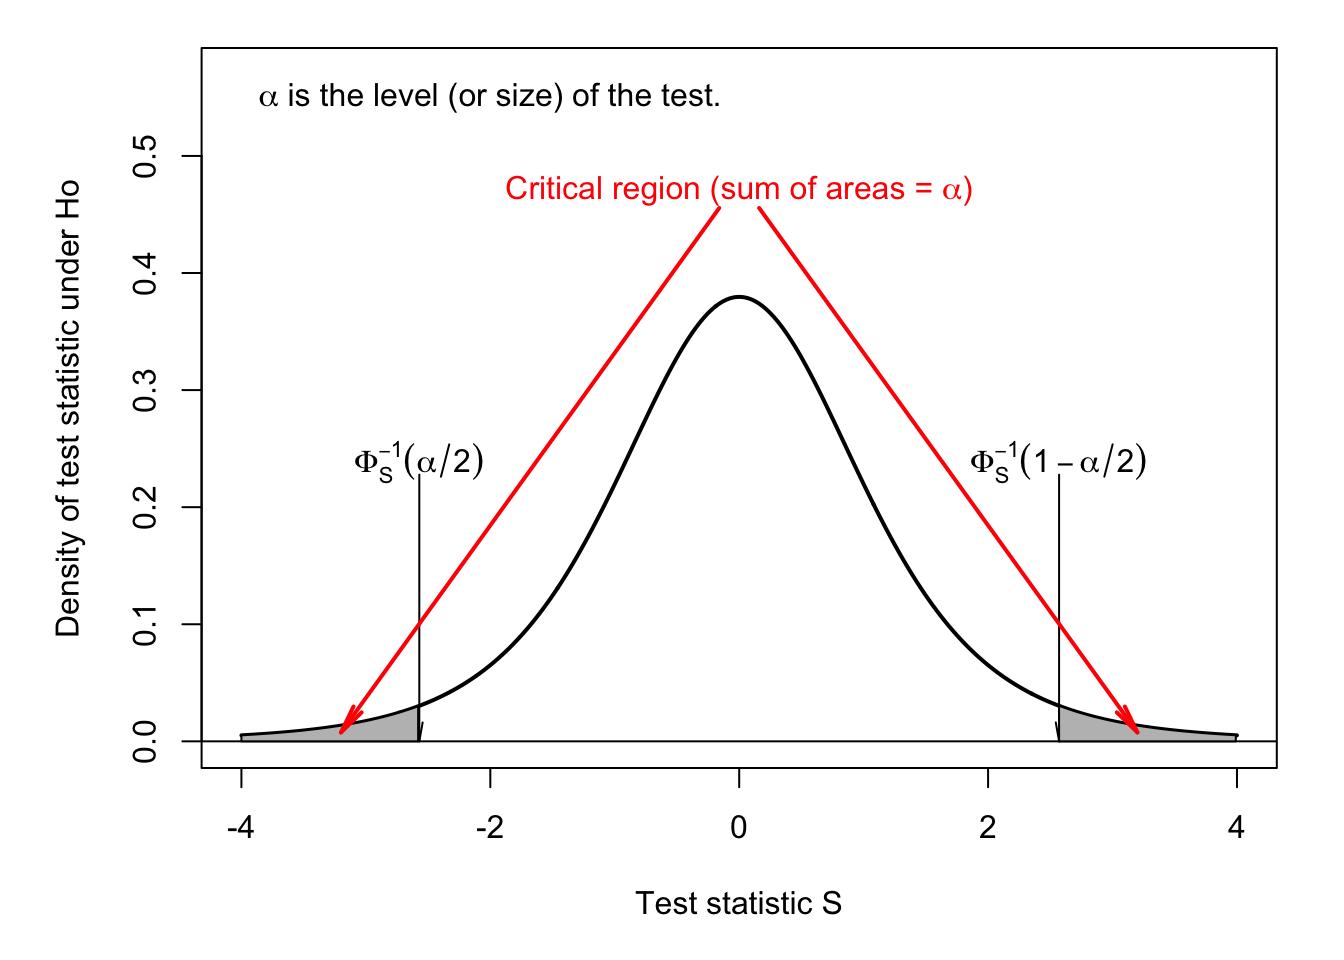
\includegraphics{EcoStat_files/figure-latex/Illusttest1-1} \caption{Two-sided test. Under $H_0$, $S \sim t(5)$. $\alpha$ is the size of the test.}\label{fig:Illusttest1}
\end{figure}

\begin{figure}
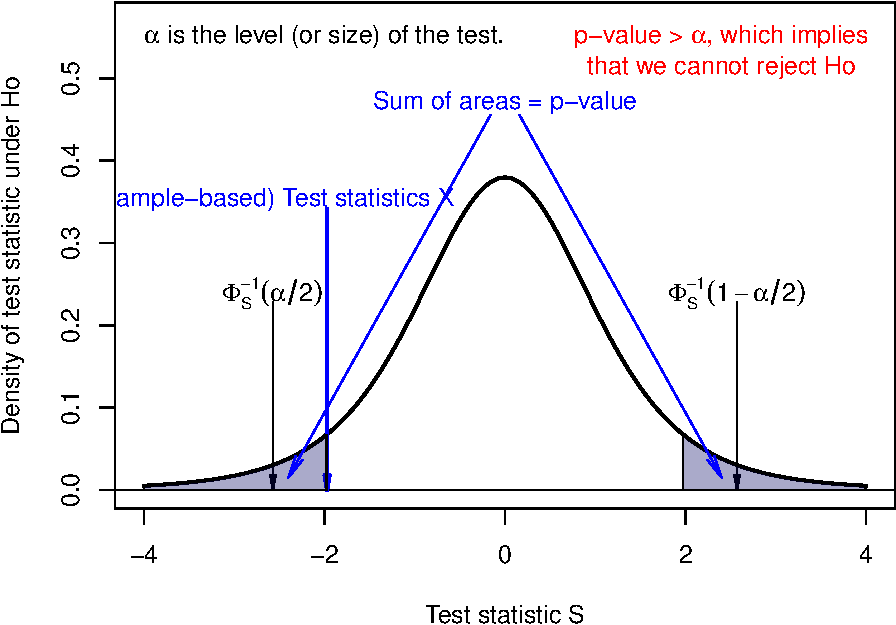
\includegraphics{EcoStat_files/figure-latex/Illusttest2-1} \caption{Two-sided test. Under $H_0$, $S \sim t(5)$. $\alpha$ is the size of the test.}\label{fig:Illusttest2}
\end{figure}

Figures \ref{fig:IllusTestOneSided1} and \ref{fig:IllusTestOneSided2} illustrate the \textbf{one-tailed}, or \textbf{one-sided} situation. These tests are typically employed when the distribution of the test statistic under the null hypothesis has a support on \(\mathbb{R}^+\) (e.g., the chi-square distribution \(\chi^2\), see Def. \ref{def:chi2}). Figure \ref{fig:IllusTestOneSided2} also illustrates the notion of p-value associated with a one-sided statistical test.

\begin{figure}
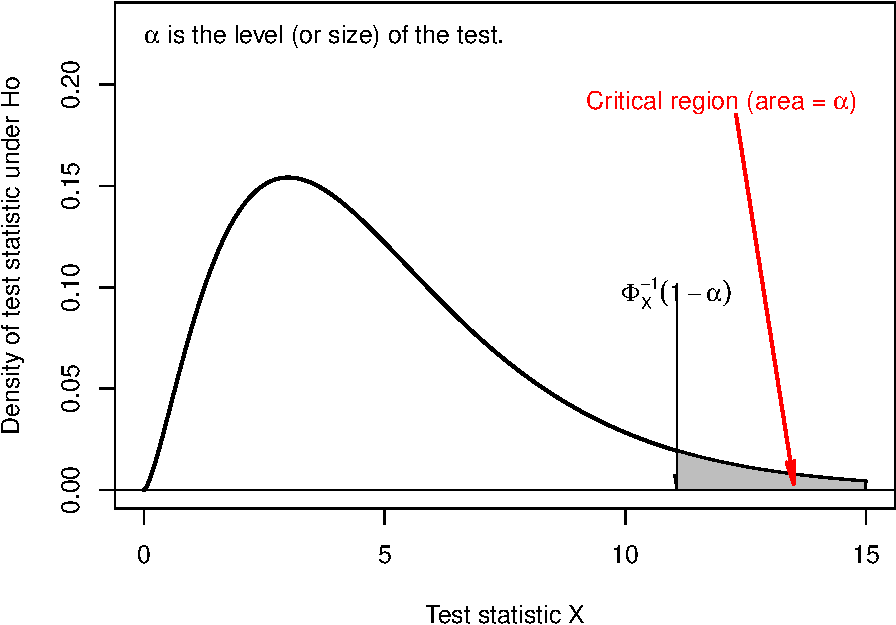
\includegraphics{EcoStat_files/figure-latex/IllusTestOneSided1-1} \caption{One-sided test. Under $H_0$, $S \sim \chi^2(5)$. $\alpha$ is the size of the test.}\label{fig:IllusTestOneSided1}
\end{figure}

\begin{figure}
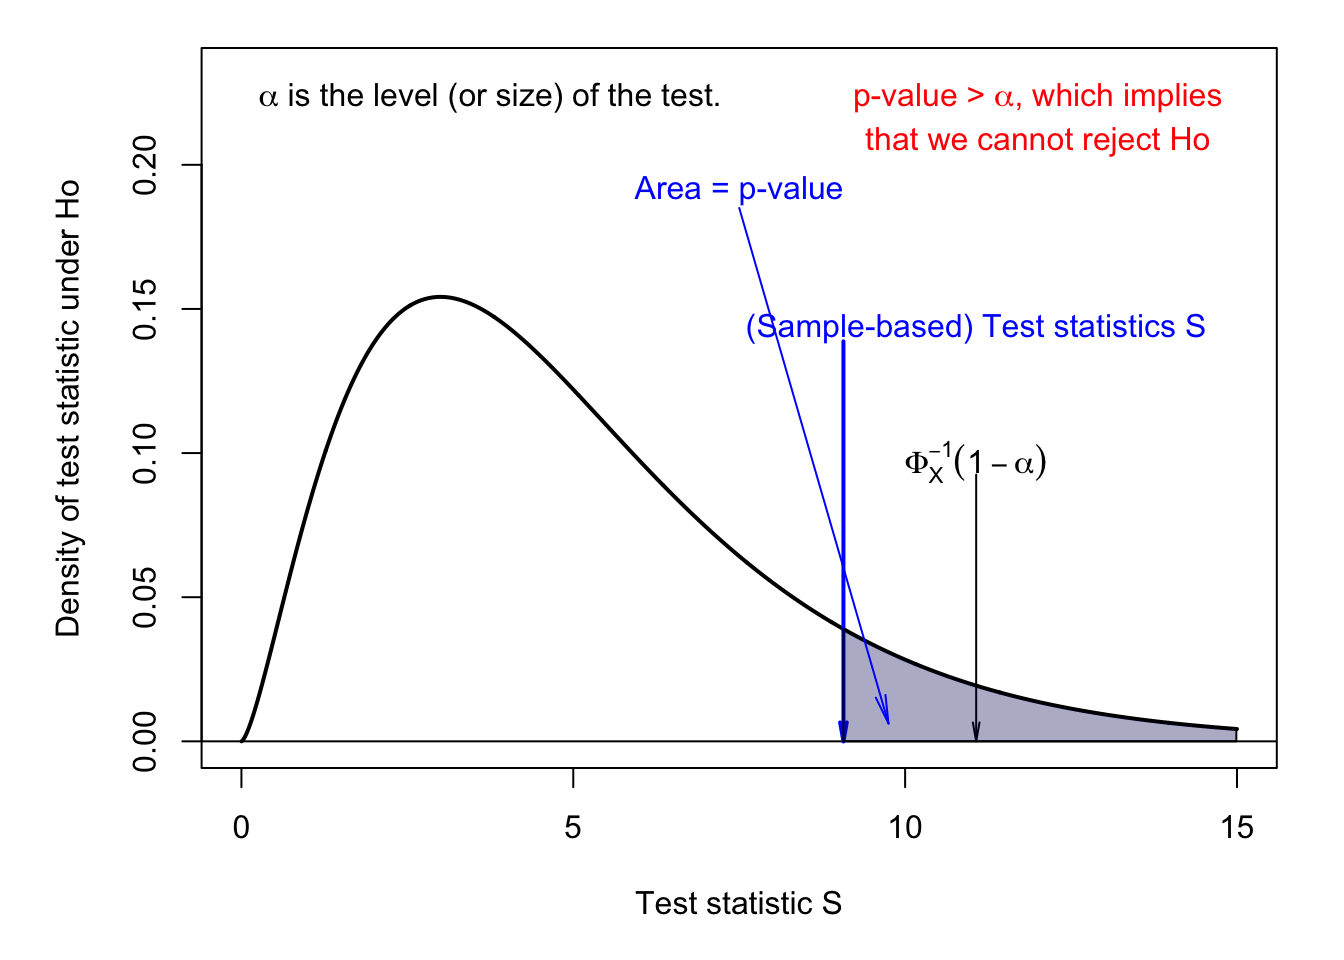
\includegraphics{EcoStat_files/figure-latex/IllusTestOneSided2-1} \caption{One-sided test. Under $H_0$, $S \sim \chi^2(5)$. $\alpha$ is the size of the test.}\label{fig:IllusTestOneSided2}
\end{figure}

\begin{example}[A practical illustration of size and power]
\protect\hypertarget{exm:Factory}{}\label{exm:Factory}Consider a factory that produces metal cylinders whose diameter has to be equal to 1,cm. The tolerance is \(a=0.01\) cm. More precisely, more than 90\% of the pieces have to satisfy the tolerance for the whole production (say 1.000.000 pieces) to be bought by the client.

The production technology is such that a proportion \(\theta\) (imperfectly known) of the pieces does not satisfy the tolerance. The (population) parameter \(\theta\) could be computed by measuring all the pieces but this would be costly. Instead, it is decided that \(n \ll 1.000.000\) pieces will be measured. In this context, the null hypothesis \(H_0\) is \(\theta < 10\%\). The producing firm would like \(H_0\) to be true.

Let us denote by \(d_i\) the binary indicator defined as:
\[
d_i = \left\{
\begin{array}{cll}
0 & \mbox{if the size of the $i^{th}$ cylinder is in $[1-a,1+a]$;}\\
1 & \mbox{otherwise.}
\end{array}
\right.
\]

We set \(x_n=\sum_{i=1}^n d_i\). That is, \(x_n\) is the number of measured pieces that do not satisfy the tolerance (out of \(n\)).

The decision rule is: accept \(H_0\) if \(\dfrac{x_n}{n} \le b\), reject otherwise. A natural choice for \(b\) is \(b=0.1\). However, this would not be a conservative choice, since it remains likely that \(x_n<0.1\) even if \(\mathbb{E}(x_n)=\theta>0.1\) (especially if \(n\) is small). Hence, if one chooses \(b=0.1\), the probability of false negative may be high.

In this simple example, the size and the power of the test can be computed analytically. The test statistic is \(S_n=\frac{x_n}{n}\) and the critical region is \(\Omega = [b,1]\). The probability to reject \(H_0\) is:
\begin{eqnarray*}
\mathbb{P}_\theta(S_n \in \Omega) = \sum_{i=b \times n+1}^{n}C_{n}^i\theta^i(1-\theta)^{n-i}.
\end{eqnarray*}

When \(\theta<0.1\), the previous expression gives the size of the test, while it gives the power of the test when \(\theta>0.1\). Figure \ref{FactoryR} shows how this probability depends on \(\theta\) for two sample sizes: \(n=100\) (upper plot) and \(n=500\) (lower plot).

\begin{figure}
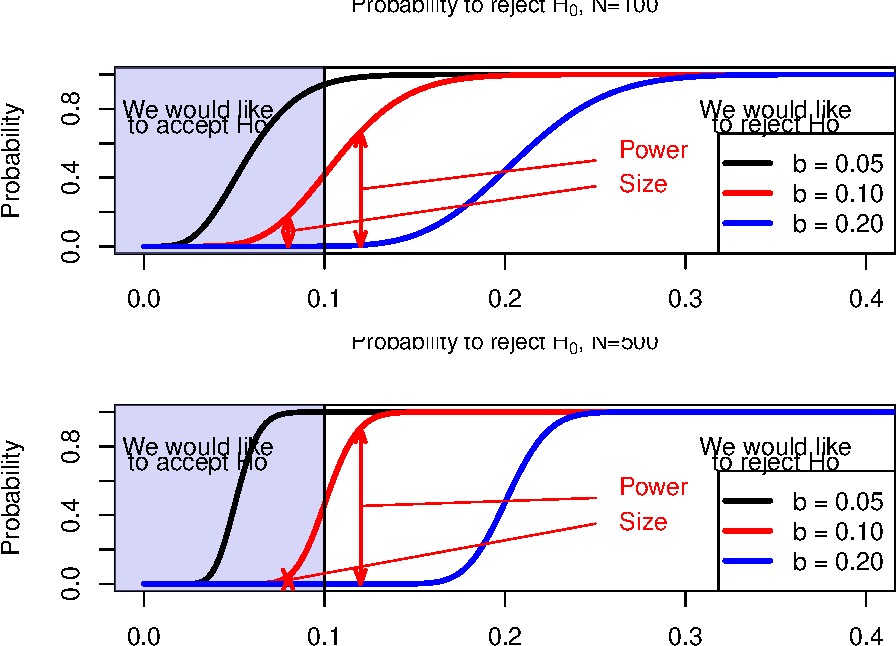
\includegraphics{EcoStat_files/figure-latex/FactoryR-1} \caption{Factory example.}\label{fig:FactoryR}
\end{figure}

(Alternative situations can be explored by using this \href{https://jrenne.shinyapps.io/Factory/}{web interface}.)
\end{example}

\hypertarget{asymptotic-properties-of-statistical-tests}{%
\section{Asymptotic properties of statistical tests}\label{asymptotic-properties-of-statistical-tests}}

In some cases, the distribution of the test statistic is known only asymptotically. For instance, it may be the case that the distribution of a given test statistic becomes normal only in large samples (e.g., related to the CLT, see Section \ref{TCL}). The level of the test is then not know for small sample sizes, but only asymptotically, i.e., when \(n\) becomes infinitely large. That defines the asymptotic level of the test:

\begin{definition}[Asymptotic level]
\protect\hypertarget{def:asmyptlevel}{}\label{def:asmyptlevel}An asymptotic test with critical region \(\Omega_n\) has an asymptotic level equal to \(\alpha\) if:
\[
\underset{\theta \in \Theta}{\mbox{sup}} \quad \underset{n \rightarrow \infty}{\mbox{lim}} \mathbb{P}_\theta (S_n \in \Omega_n) = \alpha.
\]
\end{definition}

\begin{example}[The factory example]
\protect\hypertarget{exm:FactAsymptlevel}{}\label{exm:FactAsymptlevel}Let us come back to the factory example (Example \ref{exm:Factory}). Because \(S_n =\bar{d}_n\), and since \(\mathbb{E}(d_i)=\theta\) and \(\mathbb{V}ar(d_i)=\theta(1-\theta)\), the CLT (Theorem \ref{thm:LindbergLevyCLT}) leads to:
\[
S_n \sim \mathcal{N}\left(\theta,\frac{1}{n}\theta(1-\theta)\right) \quad or \quad \frac{\sqrt{n}(S_n-\theta)}{\sqrt{\theta(1-\theta)}} \sim \mathcal{N}(0,1).
\]

Hence, \(\mathbb{P}_\theta (S_n \in \Omega_n)=\mathbb{P}_\theta (S_n > b) \approx 1-\Phi\left(\frac{\sqrt{n}(b-\theta)}{\sqrt{\theta(1-\theta)}}\right)\). Since function \(\theta \rightarrow 1-\Phi\left(\frac{\sqrt{n}(b-\theta)}{\sqrt{\theta(1-\theta)}}\right)\) increases w.r.t. \(\theta\), we have:
\[
\underset{\theta \in \Theta=[0,0.1]}{\mbox{sup}} \quad \mathbb{P}_\theta (S_n > b_n) = \mathbb{P}_{\theta=0.1} (S_n \in \Omega_n)\approx\]
\[
1-\Phi\left(\frac{\sqrt{n}(b_n-0.1)}{0.3}\right).
\]
Hence, if we set \(b_n = 0.1 + 0.3\Phi^{-1}(1-\alpha)/\sqrt{n}\), we have \({\mbox{sup}}_{\theta \in \Theta=[0,0.1]} \quad \mathbb{P}_\theta (S_n > b_n) \approx \alpha\) for large values of \(n\).
\end{example}

Let us now turn to the power of the test. Although it is often difficult to compute the power of the test, it is sometimes feasible to demonstrate that the power of the test converges to one when \(n\) goes to \(+\infty\). In that case, if \(H_0\) is false, the probability to reject it tends to be close to one in large samples.

\begin{definition}[Asymptotically consistent test]
\protect\hypertarget{def:asmyptconsisttest}{}\label{def:asmyptconsisttest}An asymptotic test with critical region \(\Omega_n\) is consistent if:
\[
\forall \theta \in \Theta^c, \quad \mathbb{P}_\theta (S_n \in \Omega_n) \rightarrow 1.
\]
\end{definition}

\begin{example}[The factory example]
\protect\hypertarget{exm:FactAsymptConsist}{}\label{exm:FactAsymptConsist}Let us come back to the factory example (Example \ref{exm:Factory}). We proceed under the assumption that \(\theta>0.1\) and we consider \(b_n = b = 0.1\). We still have:
\[
\mathbb{P}_\theta (S_n \in \Omega_n)=\mathbb{P}_\theta (S_n > b) \approx 1-\Phi\left(\frac{\sqrt{n}(b-\theta)}{\sqrt{\theta(1-\theta)}}\right).
\]

Because \(\frac{\sqrt{n}(b-\theta)}{\sqrt{\theta(1-\theta)}} \underset{n \rightarrow \infty}{\rightarrow} -\infty\), we have
\[
\mathbb{P}_\theta (S_n > b) \approx 1- \underbrace{\Phi\left(\frac{\sqrt{n}(b-\theta)}{\sqrt{\theta(1-\theta)}}\right)}_{\underset{n \rightarrow \infty}{\rightarrow} 0} \underset{n \rightarrow \infty}{\rightarrow} 1.
\]
Therefore, with \(b_n=b=0.1\), the test is consistent.
\end{example}

\hypertarget{example-normality-tests}{%
\section{Example: Normality tests}\label{example-normality-tests}}

Because many statistical results are valid only if the underlying data is normally distributed, researchers often have tu conduct normality tests. Under the null hypothesis, the data at hand (\(\mathbf{y}=\{y_1,\dots,y_n\}\), say) are drawn from a Gaussian distribution. A popular normality test is the Jarque-Bera test. It consists in verifying that the sample skewness and kurtosis of the \(y_i\)'s are consistent with those of the normal distribution. Let us first define the skewness and kurtosis of a random variable.

Let \(f\) be the p.d.f. of \(Y\). The \(k^{th}\) \textbf{standardized moment} of \(Y\) is defined as:
\[
\psi_k = \frac{\mu_k}{\left(\sqrt{\mathbb{V}ar(Y)}\right)^k},
\]
where \(\mathbb{E}(Y)=\mu\) and
\[
\mu_k = \mathbb{E}[(Y-\mu)^k]= \int_{-\infty}^{\infty} (y-\mu)^k f(y) dy
\]
is the \(k^{th}\) \textbf{central moment} of \(Y\). In particular, \(\mu_2 = \mathbb{V}ar(Y)\). Therefore:
\[
\psi_k = \frac{\mu_k}{\left(\mu_2^{1/2}\right)^k},
\]

The \textbf{skewness} of \(Y\) corresponds to \(\psi_3\) and the \textbf{kurtosis} to \(\psi_4\) (Def. \ref{def:skewnesskurtosis}).

\begin{proposition}[Skewness and kurtosis of the normal distribution]
\protect\hypertarget{prp:normSkewKurt}{}\label{prp:normSkewKurt}For a Gaussian var., the skewness (\(\psi_3\)) is 0 and the kurtosis (\(\psi_4\)) is 3.
\end{proposition}

\begin{proof}
For a centered Gaussian distribution, \((-y)^3f(-y)=-y^3f(y)\). This implies that
\begin{eqnarray*}
\int_{-\infty}^{\infty}y^3f(y)dy&=&\int_{-\infty}^{0}y^3f(y)dy+\int_{0}^{\infty}y^3f(y)dy\\
&=&-\int_{0}^{\infty}y^3f(y)dy+\int_{0}^{\infty}y^3f(y)dy=0,
\end{eqnarray*}
which leads to the skewness result.

Moreover, for a Gaussian distribution, \(df(y)/dy=-yf(y)\) and therefore \(\frac{d}{dy}(y^3f(y))=3y^2f(y)-y^4f(y)\). Partial integration leads to the kurtosis result.
\end{proof}

Let us now introduce the sample analog of standardized moments. The \(k^{th}\) \textbf{central sample moment} of \(Y\) is given by:
\[
m_k = \frac{1}{n}\sum_{i=1}^n(y_i - \bar{y})^k,
\]
and the \(k^{th}\) \textbf{standardized sample moment} of \(Y\) is given by:
\[
g_k = \frac{m_k}{m_2^{k/2}}.
\]

\begin{proposition}[Consistency of central sample moments]
\protect\hypertarget{prp:conssitCentralMoments}{}\label{prp:conssitCentralMoments}If the \(k^{th}\) central moment of \(Y\), exists and if the \(y_i\)'s are i.i.d., then the sample central moment \(m_k\) is a consistent estimate of the central moment \(\mu_k\).
\end{proposition}

\begin{proposition}[Asymptotic distribution of 3rd-order sample central moment of a normal distribution]
\protect\hypertarget{prp:Asymptg3Normal}{}\label{prp:Asymptg3Normal}If \(y_i\sim\,i.i.d.\,\mathcal{N}(\mu,\sigma^2)\), then \(\sqrt{n}g_3 \overset{d}{\rightarrow} \mathcal{N}(0,6)\).
\end{proposition}

\begin{proof}
See, e.g.~\href{http://www.springer.com/la/book/9780387985954}{Lehmann (1999)}.
\end{proof}

\begin{proposition}[Asymptotic distribution of 4th-order sample central moment of a normal distribution]
\protect\hypertarget{prp:Asymptg4Normal}{}\label{prp:Asymptg4Normal}If \(y_i\sim\,i.i.d.\,\mathcal{N}(\mu,\sigma^2)\), then \(\sqrt{n}(g_4-3) \overset{d}{\rightarrow} \mathcal{N}(0,24)\).
\end{proposition}

\begin{proposition}[Joint asymptotic distribution of 3rd and 4th-order sample central moments of a normal distribution]
\protect\hypertarget{prp:Asymptg3g4Normal}{}\label{prp:Asymptg3g4Normal}If \(y_i\sim\,i.i.d.\,\mathcal{N}(\mu,\sigma^2)\), then the vector \((\sqrt{n}g_3,\sqrt{n}(g_4-3))\) is asymptotically bivariate Gaussian. Further its elements are uncorrelated and therefore independent.
\end{proposition}

The Jarque-Bera statistic is defined by:
\[
JB = n \left( \frac{g_3^2}{6}+\frac{(g_4-3)^2}{24} \right) = \frac{n}{6}\left(g_3^2 + \frac{(g_4-3)^2}{4}\right).
\]

\begin{proposition}[Jarque-Bera asympt. distri.]
\protect\hypertarget{prp:JB}{}\label{prp:JB}If \(y_i\sim\,i.i.d.\,\mathcal{N}(\mu,\sigma^2)\), \(JB \overset{d}{\rightarrow} \chi^2(2)\).
\end{proposition}

\begin{proof}
This directly derives from Proposition \ref{prp:Asymptg3g4Normal}.
\end{proof}

\begin{example}[Consistency of the Jarque-Bera normality test]
\protect\hypertarget{exm:JB}{}\label{exm:JB}

This example illustrates the consistency of the JB test (see Def. \ref{def:asmyptconsisttest}).

For each row of matrix \texttt{x}, the function \texttt{JB} (defined below) computes the Jarque-Bera test statistic. (That is, each row is considered as a given sample.)

\begin{Shaded}
\begin{Highlighting}[]
\NormalTok{JB }\OtherTok{\textless{}{-}} \ControlFlowTok{function}\NormalTok{(x)\{}
\NormalTok{  N }\OtherTok{\textless{}{-}} \FunctionTok{dim}\NormalTok{(x)[}\DecValTok{1}\NormalTok{] }\CommentTok{\# number of samples}
\NormalTok{  n }\OtherTok{\textless{}{-}} \FunctionTok{dim}\NormalTok{(x)[}\DecValTok{2}\NormalTok{] }\CommentTok{\# sample size}
\NormalTok{  x.bar }\OtherTok{\textless{}{-}} \FunctionTok{apply}\NormalTok{(x,}\DecValTok{1}\NormalTok{,mean)}
\NormalTok{  x.x.bar }\OtherTok{\textless{}{-}}\NormalTok{ x }\SpecialCharTok{{-}} \FunctionTok{matrix}\NormalTok{(x.bar,N,n)}
\NormalTok{  m}\FloatTok{.2} \OtherTok{\textless{}{-}} \FunctionTok{apply}\NormalTok{(x.x.bar,}\DecValTok{1}\NormalTok{,}\ControlFlowTok{function}\NormalTok{(x)\{}\FunctionTok{mean}\NormalTok{(x}\SpecialCharTok{\^{}}\DecValTok{2}\NormalTok{)\})}
\NormalTok{  m}\FloatTok{.3} \OtherTok{\textless{}{-}} \FunctionTok{apply}\NormalTok{(x.x.bar,}\DecValTok{1}\NormalTok{,}\ControlFlowTok{function}\NormalTok{(x)\{}\FunctionTok{mean}\NormalTok{(x}\SpecialCharTok{\^{}}\DecValTok{3}\NormalTok{)\})}
\NormalTok{  m}\FloatTok{.4} \OtherTok{\textless{}{-}} \FunctionTok{apply}\NormalTok{(x.x.bar,}\DecValTok{1}\NormalTok{,}\ControlFlowTok{function}\NormalTok{(x)\{}\FunctionTok{mean}\NormalTok{(x}\SpecialCharTok{\^{}}\DecValTok{4}\NormalTok{)\})}
\NormalTok{  g}\FloatTok{.3} \OtherTok{\textless{}{-}}\NormalTok{ m}\FloatTok{.3}\SpecialCharTok{/}\NormalTok{m}\FloatTok{.2}\SpecialCharTok{\^{}}\NormalTok{(}\DecValTok{3}\SpecialCharTok{/}\DecValTok{2}\NormalTok{)}
\NormalTok{  g}\FloatTok{.4} \OtherTok{\textless{}{-}}\NormalTok{ m}\FloatTok{.4}\SpecialCharTok{/}\NormalTok{m}\FloatTok{.2}\SpecialCharTok{\^{}}\NormalTok{(}\DecValTok{4}\SpecialCharTok{/}\DecValTok{2}\NormalTok{)}
  \FunctionTok{return}\NormalTok{(n}\SpecialCharTok{*}\NormalTok{(g}\FloatTok{.3}\SpecialCharTok{\^{}}\DecValTok{2}\SpecialCharTok{/}\DecValTok{6} \SpecialCharTok{+}\NormalTok{ (g}\FloatTok{.4}\DecValTok{{-}3}\NormalTok{)}\SpecialCharTok{\^{}}\DecValTok{2}\SpecialCharTok{/}\DecValTok{24}\NormalTok{))}
\NormalTok{\}}
\end{Highlighting}
\end{Shaded}

Let us first consider the case where \(H_0\) is satisfied. Figure \ref{fig:JBTest2} displays, for different sample sizes \(n\), the distribution of the JB statistics when the \(y_i\)'s are normal, consistently with \(H_0\). It appears that when \(n\) grows, the distribution indeed converges to the \(\chi^2(2)\) distribution (as stated by Proposition \ref{prp:JB}).

\begin{Shaded}
\begin{Highlighting}[]
\NormalTok{all.n }\OtherTok{\textless{}{-}} \FunctionTok{c}\NormalTok{(}\DecValTok{5}\NormalTok{,}\DecValTok{10}\NormalTok{,}\DecValTok{20}\NormalTok{,}\DecValTok{100}\NormalTok{)}
\NormalTok{nb.sim }\OtherTok{\textless{}{-}} \DecValTok{10000}
\NormalTok{y }\OtherTok{\textless{}{-}} \FunctionTok{matrix}\NormalTok{(}\FunctionTok{rnorm}\NormalTok{(nb.sim}\SpecialCharTok{*}\FunctionTok{max}\NormalTok{(all.n)),nb.sim,}\FunctionTok{max}\NormalTok{(all.n))}

\FunctionTok{par}\NormalTok{(}\AttributeTok{mfrow=}\FunctionTok{c}\NormalTok{(}\DecValTok{2}\NormalTok{,}\DecValTok{2}\NormalTok{));}\FunctionTok{par}\NormalTok{(}\AttributeTok{plt=}\FunctionTok{c}\NormalTok{(.}\DecValTok{1}\NormalTok{,.}\DecValTok{95}\NormalTok{,.}\DecValTok{15}\NormalTok{,.}\DecValTok{8}\NormalTok{))}
\ControlFlowTok{for}\NormalTok{(i }\ControlFlowTok{in} \DecValTok{1}\SpecialCharTok{:}\FunctionTok{length}\NormalTok{(all.n))\{}
\NormalTok{  n }\OtherTok{\textless{}{-}}\NormalTok{ all.n[i]}
  \FunctionTok{hist}\NormalTok{(}\FunctionTok{JB}\NormalTok{(y[,}\DecValTok{1}\SpecialCharTok{:}\NormalTok{n]),}\AttributeTok{nclass =} \DecValTok{200}\NormalTok{,}\AttributeTok{freq =} \ConstantTok{FALSE}\NormalTok{,}
       \AttributeTok{main=}\FunctionTok{paste}\NormalTok{(}\StringTok{"n = "}\NormalTok{,}\FunctionTok{toString}\NormalTok{(n),}\AttributeTok{sep=}\StringTok{""}\NormalTok{),}\AttributeTok{xlim=}\FunctionTok{c}\NormalTok{(}\DecValTok{0}\NormalTok{,}\DecValTok{10}\NormalTok{))}
\NormalTok{  xx }\OtherTok{\textless{}{-}} \FunctionTok{seq}\NormalTok{(}\DecValTok{0}\NormalTok{,}\DecValTok{10}\NormalTok{,}\AttributeTok{by=}\NormalTok{.}\DecValTok{01}\NormalTok{)}
  \FunctionTok{lines}\NormalTok{(xx,}\FunctionTok{dchisq}\NormalTok{(xx,}\AttributeTok{df =} \DecValTok{2}\NormalTok{),}\AttributeTok{col=}\StringTok{"red"}\NormalTok{)}
\NormalTok{\}}
\end{Highlighting}
\end{Shaded}

\begin{figure}
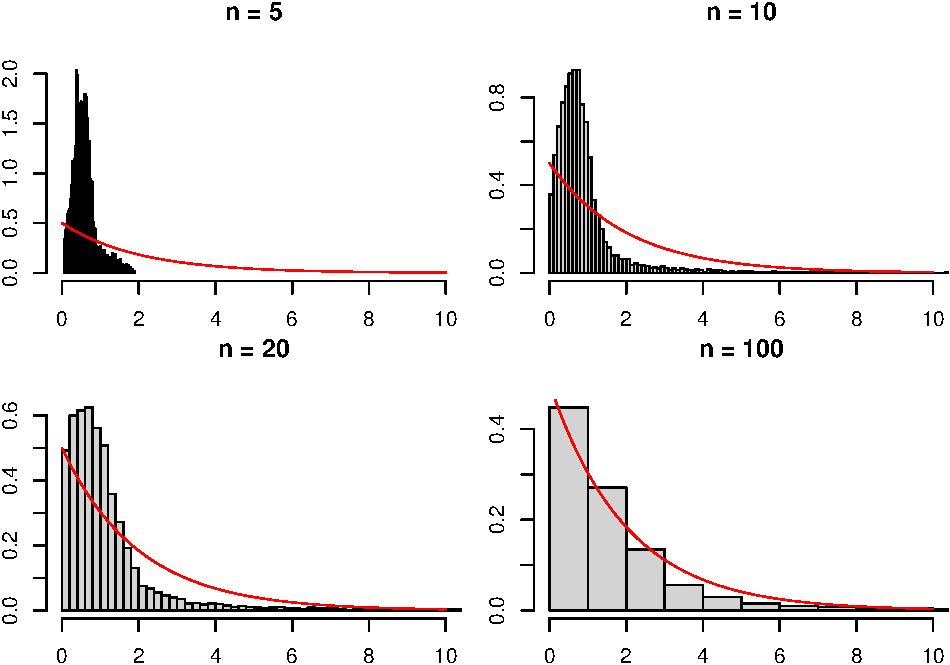
\includegraphics{EcoStat_files/figure-latex/JBTest2-1} \caption{Distribution of the JB test statistic under $H_0$ (normality).}\label{fig:JBTest2}
\end{figure}

Now, replace \texttt{rnorm} with \texttt{runif}. The \(y_i\)'s are then drawn from a uniform distribution. \(H_0\) is not satisfied. Figure \ref{fig:JBTest3} then shows that, when \(n\) grows, the distributions of the JB statistic shift to the right. This results in the consistency of the JB test (see Def. \ref{def:asmyptconsisttest}).

\begin{figure}
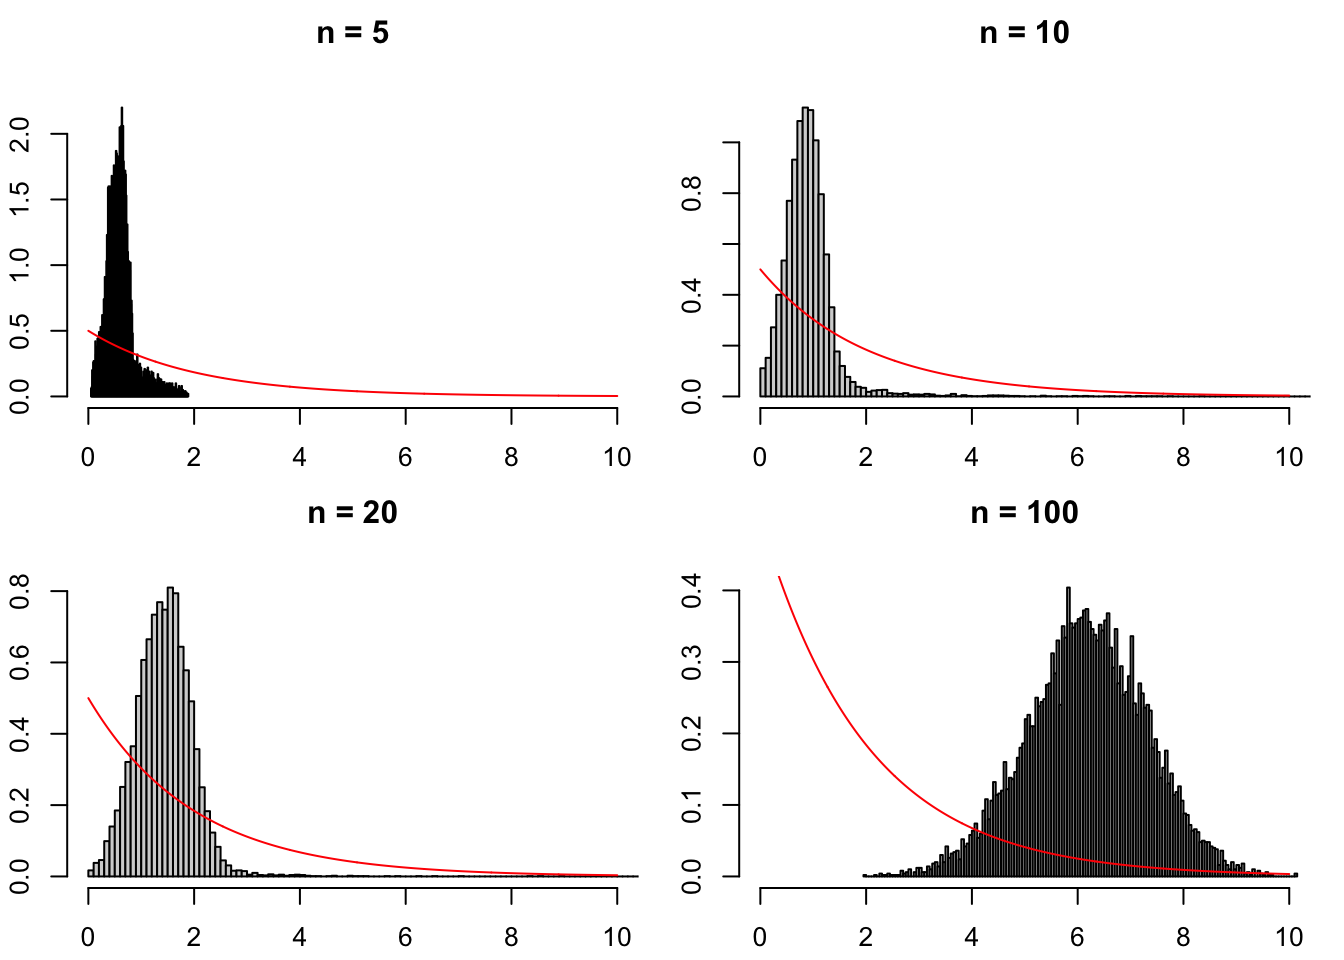
\includegraphics{EcoStat_files/figure-latex/JBTest3-1} \caption{Distribution of the JB test statistic when the $y_i$'s are drawn from a uniform distribution (hence $H_0$ is not satisfied).}\label{fig:JBTest3}
\end{figure}

\end{example}

\hypertarget{ChapterLS}{%
\chapter{Linear Regressions}\label{ChapterLS}}

\begin{definition}
\protect\hypertarget{def:essai}{}\label{def:essai}A linear regression model is of the form:
\begin{equation}
y_i = \boldsymbol\beta'\mathbf{x}_{i} + \varepsilon_i,\label{eq:linearspecif}
\end{equation}
where \(\mathbf{x}_{i}=[x_{i,1},\dots,x_{i,K}]'\) is a vector of dimension \(K \times 1\).
\end{definition}

For entity \(i\), the \(x_{i,k}\)'s, for \(k \in \{1,\dots,K\}\), are explanatory variables, regressors, or covariates. The variable of interest, \(y_i\), is often called dependent variable, or regressand. The last term of the specification, namely \(\varepsilon_i\), is called error, or disturbance.

The researcher is usually interested in the components of vector \(\boldsymbol\beta\), denoted by \(\beta_k\), \(k \in \{1,\dots,K\}\). She usually aims at estimating these coefficients based on observations of \(\{y_i,\mathbf{x}_{i}\}\), \(i \in \{1,\dots,n\}\), which constitutes a \emph{sample}. In the following, we will denote the sample length by \(n\).

To have an intercept in the specification \eqref{eq:linearspecif}, one has to set \(x_{i,1}=1\) for all \(i\); \(\beta_1\) then corresponds to the intercept.

\hypertarget{linearHyp}{%
\section{Hypotheses}\label{linearHyp}}

In this section, we introduce different assumptions regarding the covariates and/or the errors. The properties of the estimators used by the researcher depend on which of these assumptions are satisfied.

\begin{hypothesis}[Full rank]
\protect\hypertarget{hyp:fullrank}{}\label{hyp:fullrank}There is no exact linear relationship among the independent variables (the \(x_{i,k}\)'s, for a given \(i \in \{1,\dots,n\}\)).
\end{hypothesis}

Intuitively, when Hypothesis \ref{hyp:fullrank} is satisfied, then the estimation of the model parameters is unfeasible since, for any value of \(\boldsymbol\beta\), some changes in the explanatory variables will be exactly compensated by other changes in another set of explanatory variables, preventing the identification of these effects.

Let us denote by \(\mathbf{X}\) the matrix containing all explanatory variables, of dimension \(n \times K\). (That is, row \(i\) of \(\mathbf{X}\) is \(\mathbf{x}_i'\).) The following hypothesis concerns the relationship between the errors (gathered in \(\boldsymbol\varepsilon\), a \(n\)-dimensional vector) and the explanatory variables \(\mathbf{X}\):

\begin{hypothesis}[Conditional mean-zero assumption]
\protect\hypertarget{hyp:exogeneity}{}\label{hyp:exogeneity}\begin{equation}
\mathbb{E}(\boldsymbol\varepsilon|\mathbf{X}) = 0.
\end{equation}
\end{hypothesis}

Hypothesis \ref{hyp:exogeneity} has important implications:

\begin{proposition}
\protect\hypertarget{prp:implicationExog}{}\label{prp:implicationExog}

Under Hypothesis \ref{hyp:exogeneity}:

\begin{enumerate}
\def\labelenumi{\roman{enumi}.}
\tightlist
\item
  \(\mathbb{E}(\varepsilon_{i})=0\);
\item
  The \(x_{ij}\)'s and the \(\varepsilon_{i}\)'s are uncorrelated, i.e.~\(\forall i,\,j \quad \mathbb{C}orr(x_{ij},\varepsilon_{i})=0\).
\end{enumerate}

\end{proposition}

\begin{proof}

Let us prove (i) and (ii):

\begin{enumerate}
\def\labelenumi{\roman{enumi}.}
\tightlist
\item
  By the law of iterated expectations:
  \[
  \mathbb{E}(\boldsymbol\varepsilon)=\mathbb{E}(\mathbb{E}(\boldsymbol\varepsilon|\mathbf{X}))=\mathbb{E}(0)=0.
  \]
\item
  \(\mathbb{E}(x_{ij}\varepsilon_i)=\mathbb{E}(\mathbb{E}(x_{ij}\varepsilon_i|\mathbf{X}))=\mathbb{E}(x_{ij}\underbrace{\mathbb{E}(\varepsilon_i|\mathbf{X})}_{=0})=0\).
\end{enumerate}

\end{proof}

The next two hypotheses (\ref{hyp:homoskedasticity} and \ref{hyp:noncorrelResid}) concern the stochastic properties of the errors \(\varepsilon_i\):

\begin{hypothesis}[Homoskedasticity]
\protect\hypertarget{hyp:homoskedasticity}{}\label{hyp:homoskedasticity}\[
\forall i, \quad \mathbb{V}ar(\varepsilon_i|\mathbf{X}) = \sigma^2.
\]
\end{hypothesis}

The following lines of code generate a figure comparing two situations: Panel (a) of Figure \ref{fig:heteroskedasticity} corresponds to a situation of homoskedasticity, and Panel (b) corresponds to a situation of heteroskedasticity. Let us be more specific. In the two plots, we have \(X_i \sim \mathcal{N}(0,1)\) and \(\varepsilon^*_i \sim \mathcal{N}(0,1)\). In Panel (a) (homoskedasticity):
\[
Y_i = 2 + 2X_i + \varepsilon^*_i.
\]
In Panel (b) (heteroskedasticity):
\[
Y_i = 2 + 2X_i + \left(2\mathbb{I}_{\{X_i<0\}}+0.2\mathbb{I}_{\{X_i\ge0\}}\right)\varepsilon^*_i\].

\begin{Shaded}
\begin{Highlighting}[]
\NormalTok{N }\OtherTok{\textless{}{-}} \DecValTok{200}
\NormalTok{X }\OtherTok{\textless{}{-}} \FunctionTok{rnorm}\NormalTok{(N);eps }\OtherTok{\textless{}{-}} \FunctionTok{rnorm}\NormalTok{(N)}
\FunctionTok{par}\NormalTok{(}\AttributeTok{mfrow=}\FunctionTok{c}\NormalTok{(}\DecValTok{1}\NormalTok{,}\DecValTok{2}\NormalTok{),}\AttributeTok{plt=}\FunctionTok{c}\NormalTok{(.}\DecValTok{2}\NormalTok{,.}\DecValTok{95}\NormalTok{,.}\DecValTok{2}\NormalTok{,.}\DecValTok{8}\NormalTok{))}
\NormalTok{Y }\OtherTok{\textless{}{-}} \DecValTok{2} \SpecialCharTok{+} \DecValTok{2}\SpecialCharTok{*}\NormalTok{X }\SpecialCharTok{+}\NormalTok{ eps}
\FunctionTok{plot}\NormalTok{(X,Y,}\AttributeTok{pch=}\DecValTok{19}\NormalTok{,}\AttributeTok{main=}\StringTok{"(a) Homoskedasticity"}\NormalTok{,}
     \AttributeTok{las=}\DecValTok{1}\NormalTok{,}\AttributeTok{cex.lab=}\NormalTok{.}\DecValTok{8}\NormalTok{,}\AttributeTok{cex.axis=}\NormalTok{.}\DecValTok{8}\NormalTok{,}\AttributeTok{cex.main=}\NormalTok{.}\DecValTok{8}\NormalTok{,)}
\NormalTok{Y }\OtherTok{\textless{}{-}} \DecValTok{2} \SpecialCharTok{+} \DecValTok{2}\SpecialCharTok{*}\NormalTok{X }\SpecialCharTok{+}\NormalTok{ eps}\SpecialCharTok{*}\NormalTok{( (X}\SpecialCharTok{\textless{}}\DecValTok{0}\NormalTok{)}\SpecialCharTok{*}\DecValTok{2} \SpecialCharTok{+}\NormalTok{ (X}\SpecialCharTok{\textgreater{}=}\DecValTok{0}\NormalTok{)}\SpecialCharTok{*}\NormalTok{.}\DecValTok{2}\NormalTok{ )}
\FunctionTok{plot}\NormalTok{(X,Y,}\AttributeTok{pch=}\DecValTok{19}\NormalTok{,}\AttributeTok{main=}\StringTok{"(b) Heteroskedasticity"}\NormalTok{,}
     \AttributeTok{las=}\DecValTok{1}\NormalTok{,}\AttributeTok{cex.lab=}\NormalTok{.}\DecValTok{8}\NormalTok{,}\AttributeTok{cex.axis=}\NormalTok{.}\DecValTok{8}\NormalTok{,}\AttributeTok{cex.main=}\NormalTok{.}\DecValTok{8}\NormalTok{,)}
\end{Highlighting}
\end{Shaded}

\begin{figure}
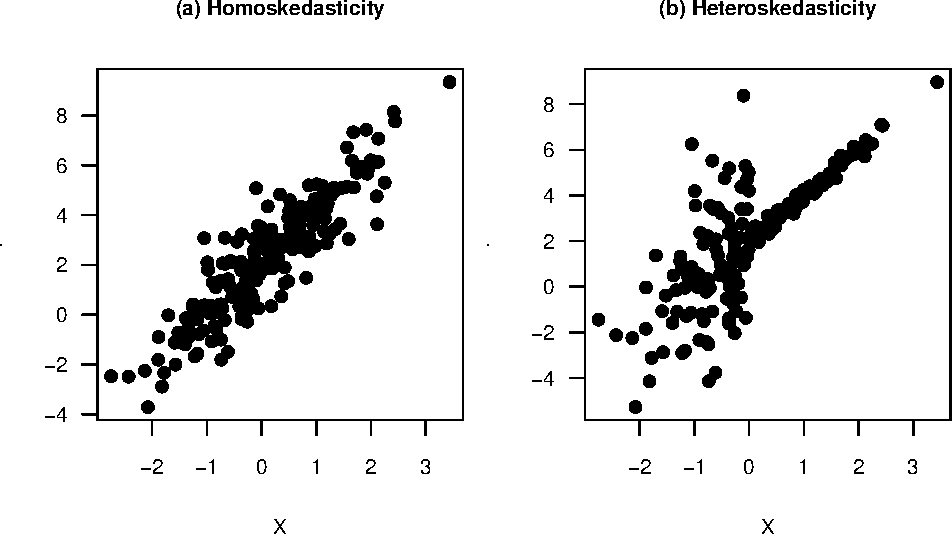
\includegraphics[width=0.9\linewidth]{EcoStat_files/figure-latex/heteroskedasticity-1} \caption{Homoskedasticity vs heteroskedasticity. See text for the exact specifications.}\label{fig:heteroskedasticity}
\end{figure}

Figure \ref{fig:exmpSalarayPhDSHP} shows a real-data situation of heteroskedasticity, based on data taken from the \href{https://forscenter.ch/projects/swiss-household-panel/}{Swiss Household Panel}. The sample is restricted to persons (i) that are younger than 35 year in 2019, and (ii) that have completed at least 19 years of study. The figure shows that the dispersion of yearly income increases with age.

\begin{Shaded}
\begin{Highlighting}[]
\FunctionTok{library}\NormalTok{(AEC)}
\FunctionTok{table}\NormalTok{(shp}\SpecialCharTok{$}\NormalTok{edyear19)}
\end{Highlighting}
\end{Shaded}

\begin{verbatim}
## 
##    8    9   10   12   13   14   16   19   21 
##   70  325  350 1985  454  117  990 1263  168
\end{verbatim}

\begin{Shaded}
\begin{Highlighting}[]
\NormalTok{shp\_higherEd }\OtherTok{\textless{}{-}} \FunctionTok{subset}\NormalTok{(shp,(edyear19}\SpecialCharTok{\textgreater{}}\DecValTok{18}\NormalTok{)}\SpecialCharTok{\&}\NormalTok{age19}\SpecialCharTok{\textless{}}\DecValTok{35}\NormalTok{)}
\FunctionTok{plot}\NormalTok{(i19wyg}\SpecialCharTok{/}\DecValTok{1000}\SpecialCharTok{\textasciitilde{}}\NormalTok{age19,}\AttributeTok{data=}\NormalTok{shp\_higherEd,}\AttributeTok{pch=}\DecValTok{19}\NormalTok{,}\AttributeTok{las=}\DecValTok{1}\NormalTok{,}
     \AttributeTok{xlab=}\StringTok{"Age"}\NormalTok{,}\AttributeTok{ylab=}\StringTok{"Yearly work income"}\NormalTok{)}
\FunctionTok{abline}\NormalTok{(}\FunctionTok{lm}\NormalTok{(i19wyg}\SpecialCharTok{/}\DecValTok{1000}\SpecialCharTok{\textasciitilde{}}\NormalTok{age19,}\AttributeTok{data=}\NormalTok{shp\_higherEd),}\AttributeTok{col=}\StringTok{"red"}\NormalTok{,}\AttributeTok{lwd=}\DecValTok{2}\NormalTok{)}
\end{Highlighting}
\end{Shaded}

\begin{figure}
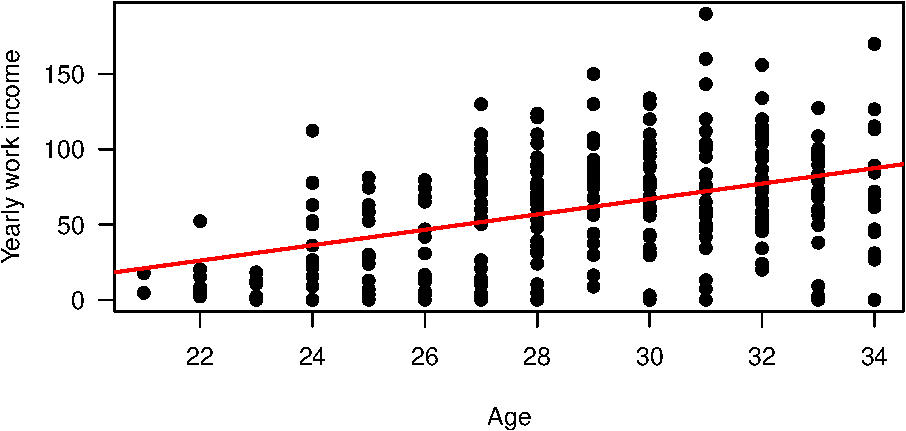
\includegraphics[width=0.95\linewidth]{EcoStat_files/figure-latex/exmpSalarayPhDSHP-1} \caption{Income versus age. Data are from the Swiss Household Panel. The sample is restricted to persons that have completed at least 19 years of study. The figure shows that the dispersion of yearly income increases with age.}\label{fig:exmpSalarayPhDSHP}
\end{figure}

The next assumption concerns the correlation of the errors across entities.

\begin{hypothesis}[Uncorrelated errors]
\protect\hypertarget{hyp:noncorrelResid}{}\label{hyp:noncorrelResid}\[
\forall i \ne j, \quad \mathbb{C}ov(\varepsilon_i,\varepsilon_j|\mathbf{X})=0.
\]
\end{hypothesis}

We will often need to work with the covariance matrix of the errors. Proposition \ref{prp:Sigma} give the specific form of the covariance matrix of the errors ---conditional on \(\mathbf{X}\)--- when both Hypotheses \ref{hyp:homoskedasticity} and \ref{hyp:noncorrelResid} are satisfied:

\begin{proposition}
\protect\hypertarget{prp:Sigma}{}\label{prp:Sigma}If Hypotheses \ref{hyp:homoskedasticity} and \ref{hyp:noncorrelResid} hold, then:
\[
\mathbb{V}ar(\boldsymbol\varepsilon|\mathbf{X})= \sigma^2 Id,
\]
where \(Id\) is the \(n \times n\) identity matrix.
\end{proposition}

We will sometimes assume that errors are Gaussian---or normal. We will then invoke Hypothesis \ref{hyp:normality}:

\begin{hypothesis}[Normal distribution]
\protect\hypertarget{hyp:normality}{}\label{hyp:normality}\[
\forall i, \quad \varepsilon_i \sim \mathcal{N}(0,\sigma^2).
\]
\end{hypothesis}

\hypertarget{LSquares}{%
\section{Least square estimation}\label{LSquares}}

\hypertarget{derivation-of-the-ols-formula}{%
\subsection{Derivation of the OLS formula}\label{derivation-of-the-ols-formula}}

In this section, we will present and study the properties of the most popular estimation approach, namely the \textbf{Ordinary Least Squares (OLS)} approach. As suggested by its name, the OLS estimator of \(\boldsymbol\beta\) is defined as the vector \(\mathbf{b}\) that minimizes the sum of squared residuals. (The \emph{residuals} are the estimates of the \emph{errors} \(\varepsilon_i\).)

For a given vector of coefficients \(\mathbf{b}=[b_1,\dots,b_K]'\), the sum of squared residuals is:
\[
f(\mathbf{b}) =\sum_{i=1}^n \left(y_i - \sum_{j=1}^K x_{i,j} b_j \right)^2 = \sum_{i=1}^n (y_i - \mathbf{x}_i' \mathbf{b})^2.
\]
Minimizing this sum amounts to minimizing:
\[
f(\mathbf{b}) = (\mathbf{y} - \mathbf{X}\mathbf{b})'(\mathbf{y} - \mathbf{X}\mathbf{b}).
\]

Since:\footnote{see Proposition \ref{prp:partial}.}
\[
\frac{\partial f}{\partial \mathbf{b}}(\mathbf{b}) = - 2 \mathbf{X}'\mathbf{y} + 2 \mathbf{X}'\mathbf{X}\mathbf{b},
\]
it comes that a necessary first-order condition (FOC) is:
\begin{equation}
\mathbf{X}'\mathbf{X}\mathbf{b} = \mathbf{X}'\mathbf{y}.\label{eq:OLSFOC}
\end{equation}
Under Assumption \ref{hyp:fullrank}, \(\mathbf{X}'\mathbf{X}\) is invertible. Hence:
\[
\boxed{\mathbf{b} = (\mathbf{X}'\mathbf{X})^{-1} \mathbf{X}'\mathbf{y}.}
\]
Vector \(\mathbf{b}\) minimizes the sum of squared residuals. (\(f\) is a non-negative quadratic function, it therefore admits a minimum.)

We have:
\[
\mathbf{y} = \underbrace{\mathbf{X}\mathbf{b}}_{\mbox{fitted values } (\hat{\mathbf{y}})} + \underbrace{\mathbf{e}}_{\mbox{residuals}}
\]

The estimated residuals are:
\begin{equation}
\mathbf{e} = \mathbf{y} - \mathbf{X} (\mathbf{X}'\mathbf{X})^{-1} \mathbf{X}' \mathbf{y} = \mathbf{M} \mathbf{y},\label{eq:Mres}
\end{equation}
where \(\mathbf{M} := \mathbf{I} - \mathbf{X} (\mathbf{X}'\mathbf{X})^{-1} \mathbf{X}'\) is called the \textbf{residual maker} matrix.

Moreover, the fitted values \(\hat{\mathbf{y}}\) are given by:
\begin{equation}
\hat{\mathbf{y}}=\mathbf{X} (\mathbf{X}'\mathbf{X})^{-1} \mathbf{X}' \mathbf{y} = \mathbf{P} \mathbf{y},\label{eq:Proj}
\end{equation}
where \(\mathbf{P}=\mathbf{X} (\mathbf{X}'\mathbf{X})^{-1} \mathbf{X}'\) is a \textbf{projection matrix}.

These matrices \(\mathbf{M}\) and \(\mathbf{P}\) are such that:

\begin{itemize}
\tightlist
\item
  \(\mathbf{M} \mathbf{X} = \mathbf{0}\): if one regresses one of the explanatory variables on \(\mathbf{X}\), the residuals are null.
\item
  \(\mathbf{M}\mathbf{y}=\mathbf{M}\boldsymbol\varepsilon\) (because \(\mathbf{y} = \mathbf{X}\boldsymbol\beta + \boldsymbol\varepsilon\) and \(\mathbf{M} \mathbf{X} = \mathbf{0}\)).
\end{itemize}

Here are some additional properties of \(\mathbf{M}\) and \(\mathbf{P}\):

\begin{itemize}
\tightlist
\item
  \(\mathbf{M}\) is symmetric (\(\mathbf{M} = \mathbf{M}'\)) and idempotent (\(\mathbf{M} = \mathbf{M}^2 = \mathbf{M}^k\) for \(k>0\)).
\item
  \(\mathbf{P}\) is symmetric and idempotent.
\item
  \(\mathbf{P}\mathbf{X} = \mathbf{X}\).
\item
  \(\mathbf{P} \mathbf{M} = \mathbf{M} \mathbf{P} = 0\).
\item
  \(\mathbf{y} = \mathbf{P}\mathbf{y} + \mathbf{M}\mathbf{y}\) (decomposition of \(\mathbf{y}\) into two orthogonal parts).
\end{itemize}

It is easily checked that \(\mathbf{X}'\mathbf{e}=0\). Each column of \(\mathbf{X}\) is therefore orthogonal to \(\mathbf{e}\). In particular, if an intercept is included in the regression (\(x_{i,1} \equiv 1\) for all \(i\)'s, i.e., the first column of \(\mathbf{X}\) is filled with ones), the average of the residuals is null.

\begin{example}[Bivariate case]
\protect\hypertarget{exm:bivar}{}\label{exm:bivar}Consider a bivariate situation, where we regress \(y_i\) on a constant and an explanatory variable \(w_i\). We have \(K=2\), and \(\mathbf{X}\) is a \(n \times 2\) matrix whose \(i^{th}\) row is \([x_{i,1},x_{i,2}]\), with \(x_{i,1}=1\) (to account for the intercept) and with \(w_i = x_{i,2}\) (say).

We have:
\begin{eqnarray*}
\mathbf{X}'\mathbf{X} &=& 
\left[\begin{array}{cc}
n & \sum_i w_i \\
\sum_i w_i & \sum_i w_i^2
\end{array}
\right],\\
(\mathbf{X}'\mathbf{X})^{-1} &=& 
\frac{1}{n\sum_i w_i^2-(\sum_i w_i)^2}
\left[\begin{array}{cc}
\sum_i w_i^2 & -\sum_i w_i \\
-\sum_i w_i & n
\end{array}
\right],\\
(\mathbf{X}'\mathbf{X})^{-1}\mathbf{X}'\mathbf{y} &=& 
\frac{1}{n\sum_i w_i^2-(\sum_i w_i)^2}
\left[\begin{array}{c}
\sum_i w_i^2\sum_i y_i -\sum_i w_i \sum_i w_iy_i \\
-\sum_i w_i \sum_i y_i + n \sum_i w_i y_i
\end{array}
\right]\\
&=& \frac{1}{\frac{1}{n}\sum_i(w_i - \bar{w})^2}
\left[\begin{array}{c}
\frac{\bar{y}}{n}\sum_i w_i^2 -\frac{\bar{w}}{n}\sum_i w_iy_i \\
\frac{1}{n}\sum_i (w_i-\bar{w})(y_i-\bar{y})
\end{array}
\right].
\end{eqnarray*}

It can be seen that the second element of \(\mathbf{b}=(\mathbf{X}'\mathbf{X})^{-1}\mathbf{X}'\mathbf{y}\) is:
\[
b_2 = \frac{\overline{\mathbb{C}ov(W,Y)}}{\overline{\mathbb{V}ar(W)}},
\]
where \(\overline{\mathbb{C}ov(W,Y)}\) and \(\overline{\mathbb{V}ar(W)}\) are sample estimates.

Since there is a constant in the regression, we have \(b_1 = \bar{y} - b_2 \bar{w}\).
\end{example}

\hypertarget{properties-of-the-ols-estimate-small-sample}{%
\subsection{Properties of the OLS estimate (small sample)}\label{properties-of-the-ols-estimate-small-sample}}

The OLS properties stated in Proposition \ref{prp:propOLS} are valid for any sample size \(n\):

\begin{proposition}[Properties of the OLS estimator]
\protect\hypertarget{prp:propOLS}{}\label{prp:propOLS}

We have:

\begin{enumerate}
\def\labelenumi{\roman{enumi}.}
\item
  Under Assumptions \ref{hyp:fullrank} and \ref{hyp:exogeneity}, the OLS estimator is linear and unbiased.
\item
  Under Hypotheses \ref{hyp:fullrank} to \ref{hyp:noncorrelResid}, the conditional covariance matrix of \(\mathbf{b}\) is: \(\mathbb{V}ar(\mathbf{b}|\mathbf{X}) = \sigma^2 (\mathbf{X}'\mathbf{X})^{-1}\).
\end{enumerate}

\end{proposition}

\begin{proof}

Under Hypothesis \ref{hyp:fullrank}, \(\mathbf{X}'\mathbf{X}\) can be inverted. We have:
\[
\mathbf{b} = (\mathbf{X}'\mathbf{X})^{-1} \mathbf{X}'\mathbf{y} = \boldsymbol\beta + (\mathbf{X}'\mathbf{X})^{-1} \mathbf{X}' \mathbf{\varepsilon}.
\]

\begin{enumerate}
\def\labelenumi{\roman{enumi}.}
\tightlist
\item
  Let us consider the expectation of the last term, i.e.~\(\mathbb{E}((\mathbf{X}'\mathbf{X})^{-1} \mathbf{X}' \mathbf{\varepsilon})\). Using the law of iterated expectations, we obtain:
  \[
  \mathbb{E}((\mathbf{X}'\mathbf{X})^{-1} \mathbf{X}' \mathbf{\varepsilon}) = \mathbb{E}(\mathbb{E}[(\mathbf{X}'\mathbf{X})^{-1} \mathbf{X}' \mathbf{\varepsilon}|\mathbf{X}]) = \mathbb{E}((\mathbf{X}'\mathbf{X})^{-1} \mathbf{X}'\mathbb{E}[\mathbf{\varepsilon}|\mathbf{X}]).
  \]
  By Hypothesis \ref{hyp:exogeneity}, we have \(\mathbb{E}[\mathbf{\varepsilon}|\mathbf{X}]=0\). Hence \(\mathbb{E}((\mathbf{X}'\mathbf{X})^{-1} \mathbf{X}' \mathbf{\varepsilon}) =0\) and result (i) follows.
\item
  \(\mathbb{V}ar(\mathbf{b}|\mathbf{X}) = (\mathbf{X}'\mathbf{X})^{-1} \mathbf{X}' \mathbb{E}(\boldsymbol\varepsilon\boldsymbol\varepsilon'|\mathbf{X}) \mathbf{X} (\mathbf{X}'\mathbf{X})^{-1}\).
  By Prop. \ref{prp:Sigma}, if \ref{hyp:homoskedasticity} and \ref{hyp:noncorrelResid} hold, then we have \(\mathbb{E}(\boldsymbol\varepsilon\boldsymbol\varepsilon'|\mathbf{X})=\mathbb{V}ar(\boldsymbol\varepsilon|\mathbf{X})=\sigma^2 Id\).
\end{enumerate}

\end{proof}

Together, Hypotheses \ref{hyp:fullrank} to \ref{hyp:noncorrelResid} form the so-called Gauss-Markov set of assumptions. Under these assumptions, the OLS estimator feature the lowest possible variance within the family of linear unbiased estimates of \(\boldsymbol\beta\):

\begin{theorem}[Gauss-Markov Theorem]
\protect\hypertarget{thm:GaussMarkov}{}\label{thm:GaussMarkov}Under Assumptions \ref{hyp:fullrank} to \ref{hyp:noncorrelResid}, for any vector \(w\), the minimum-variance linear unbiased estimator of \(w' \boldsymbol\beta\) is \(w' \mathbf{b}\), where \(\mathbf{b}\) is the least squares estimator. (BLUE: Best Linear Unbiased Estimator.)
\end{theorem}

\begin{proof}
Consider \(\mathbf{b}^* = C \mathbf{y}\), another linear unbiased estimator of \(\boldsymbol\beta\). Since it is unbiased, we must have \(\mathbb{E}(C\mathbf{y}|\mathbf{X}) = \mathbb{E}(C\mathbf{X}\boldsymbol\beta + C\boldsymbol\varepsilon|\mathbf{X}) = \boldsymbol\beta\). We have \(\mathbb{E}(C\boldsymbol\varepsilon|\mathbf{X})=C\mathbb{E}(\boldsymbol\varepsilon|\mathbf{X})=0\) (by \ref{hyp:exogeneity}). Therefore \(\mathbf{b}^*\) is unbiased if \(\mathbb{E}(C\mathbf{X})\boldsymbol\beta=\boldsymbol\beta\). This has to be the case for any \(\boldsymbol\beta\), which implies that we must have \(C\mathbf{X}=\mathbf{I}\). Let us compute \(\mathbb{V}ar(\mathbf{b^*}|\mathbf{X})\). For this, we introduce \(D = C - (\mathbf{X}'\mathbf{X})^{-1}\mathbf{X}'\), which is such that \(D\mathbf{y}=\mathbf{b}^*-\mathbf{b}\). The fact that \(C\mathbf{X}=\mathbf{I}\) implies that \(D\mathbf{X} = \mathbf{0}\). We have \(\mathbb{V}ar(\mathbf{b^*}|\mathbf{X}) = \mathbb{V}ar(C \mathbf{y}|\mathbf{X}) =\mathbb{V}ar(C \boldsymbol\varepsilon|\mathbf{X}) = \sigma^2CC'\) (by Assumptions \ref{hyp:homoskedasticity} and \ref{hyp:noncorrelResid}, see Prop. \ref{prp:Sigma}). Using \(C=D+(\mathbf{X}'\mathbf{X})^{-1}\mathbf{X}'\) and exploiting the fact that \(D\mathbf{X} = \mathbf{0}\) leads to:
\[
\mathbb{V}ar(\mathbf{b^*}|\mathbf{X}) =\sigma^2\left[(D+(\mathbf{X}'\mathbf{X})^{-1}\mathbf{X}')(D+(\mathbf{X}'\mathbf{X})^{-1}\mathbf{X}')'\right] = \mathbb{V}ar(\mathbf{b}|\mathbf{X}) + \sigma^2 \mathbf{D}\mathbf{D}'.
\]
Therefore, we have
\begin{eqnarray*}
&&\mathbb{V}ar(w'\mathbf{b^*}|\mathbf{X})=w'\mathbb{V}ar(\mathbf{b}|\mathbf{X})w + \sigma^2 w'\mathbf{D}\mathbf{D}'w\\
&\ge& w'\mathbb{V}ar(\mathbf{b}|\mathbf{X})w=\mathbb{V}ar(w'\mathbf{b}|\mathbf{X}).
\end{eqnarray*}
\end{proof}

The Frish-Waugh theorem (Theorem \ref{thm:FW}) reveals the relationship between the OLS estimator and the notion of partial correlation coefficient. Consider the linear least square regression of \(\mathbf{y}\) on \(\mathbf{X}\). We introduce the notations:

\begin{itemize}
\tightlist
\item
  \(\mathbf{b}^{\mathbf{y}/\mathbf{X}}\): OLS estimates of \(\boldsymbol\beta\),
\item
  \(\mathbf{M}^{\mathbf{X}}\): residual-maker matrix of any regression on \(\mathbf{X}\) (given by \(\mathbf{I} - \mathbf{X} (\mathbf{X}'\mathbf{X})^{-1} \mathbf{X}'\)),
\item
  \(\mathbf{P}^{\mathbf{X}}\): projection matrix of any regression on \(\mathbf{X}\) (given by \(\mathbf{X} (\mathbf{X}'\mathbf{X})^{-1} \mathbf{X}'\)).
\end{itemize}

Let us split the set of explanatory variables into two: \(\mathbf{X} = [\mathbf{X}_1,\mathbf{X}_2]\). With obvious notations: \(\mathbf{b}^{\mathbf{y}/\mathbf{X}}=[\mathbf{b}_1',\mathbf{b}_2']'\).

\begin{theorem}[Frisch-Waugh Theorem]
\protect\hypertarget{thm:FW}{}\label{thm:FW}We have:
\[
\mathbf{b}_2 = \mathbf{b}^{\mathbf{M^{\mathbf{X}_1}y}/\mathbf{M^{\mathbf{X}_1}\mathbf{X}_2}}.
\]
\end{theorem}

\begin{proof}
The minimization of the least squares leads to (these are first-order conditions, see Eq. \eqref{eq:OLSFOC}):
\[
\left[ \begin{array}{cc} \mathbf{X}_1'\mathbf{X}_1 & \mathbf{X}_1'\mathbf{X}_2 \\ \mathbf{X}_2'\mathbf{X}_1 & \mathbf{X}_2'\mathbf{X}_2\end{array}\right]
\left[ \begin{array}{c} \mathbf{b}_1 \\ \mathbf{b}_2\end{array}\right] =
\left[ \begin{array}{c} \mathbf{X}_1' \mathbf{y} \\ \mathbf{X}_2' \mathbf{y} \end{array}\right].
\]
Use the first-row block of equations to solve for \(\mathbf{b}_1\) first; it comes as a function of \(\mathbf{b}_2\). Then use the second set of equations to solve for \(\mathbf{b}_2\), which leads to:
\begin{eqnarray*}
\mathbf{b}_2 &=& [\mathbf{X}_2'\mathbf{X}_2 - \mathbf{X}_2'\mathbf{X}_1(\mathbf{X}_1'\mathbf{X}_1)\mathbf{X}_1'\mathbf{X}_2]^{-1}\mathbf{X}_2'(Id - \mathbf{X}_1(\mathbf{X}_1'\mathbf{X}_1)\mathbf{X}_1')\mathbf{y}\\
&=& [\mathbf{X}_2' \mathbf{M}^{\mathbf{X}_1}\mathbf{X}_2]^{-1}\mathbf{X}_2'\mathbf{M}^{\mathbf{X}_1}\mathbf{y}.
\end{eqnarray*}
Using the fact that \(\mathbf{M}^{\mathbf{X}_1}\) is idempotent and symmetric leads to the result.
\end{proof}

This suggests a second way of estimating \(\mathbf{b}_2\):

\begin{enumerate}
\def\labelenumi{\arabic{enumi}.}
\tightlist
\item
  Regress \(Y\) on \(X_1\), regress \(X_2\) on \(X_1\).
\item
  Regress the residuals associated with the former regression on those associated with the latter regressions.
\end{enumerate}

This is illustrated by the following code, where we run different regressions involving the number of Google searches for ``parapluie'' (\emph{umbrella} in French). In the broad specification, we regress it on French precipitations and month dummies. Next, we deseasonalize both the dependent variable and the precipitations by regressing them on the month dummies. As stated by Theorem \ref{thm:FW}, regressing deseasonalized Google searches on deseasonalized precipitations give the same coefficient as in the baseline regression.

\begin{Shaded}
\begin{Highlighting}[]
\FunctionTok{library}\NormalTok{(AEC)}
\NormalTok{dummies }\OtherTok{\textless{}{-}} \FunctionTok{as.matrix}\NormalTok{(parapluie[,}\DecValTok{4}\SpecialCharTok{:}\DecValTok{14}\NormalTok{])}
\NormalTok{eq\_all }\OtherTok{\textless{}{-}} \FunctionTok{lm}\NormalTok{(parapluie}\SpecialCharTok{\textasciitilde{}}\NormalTok{dummies}\SpecialCharTok{+}\NormalTok{precip,}\AttributeTok{data=}\NormalTok{parapluie)}
\NormalTok{deseas\_parapluie }\OtherTok{\textless{}{-}} \FunctionTok{lm}\NormalTok{(parapluie}\SpecialCharTok{\textasciitilde{}}\NormalTok{dummies,}\AttributeTok{data=}\NormalTok{parapluie)}\SpecialCharTok{$}\NormalTok{residuals}
\NormalTok{deseas\_precip    }\OtherTok{\textless{}{-}} \FunctionTok{lm}\NormalTok{(precip}\SpecialCharTok{\textasciitilde{}}\NormalTok{dummies,}\AttributeTok{data=}\NormalTok{parapluie)}\SpecialCharTok{$}\NormalTok{residuals}
\NormalTok{eq\_frac }\OtherTok{\textless{}{-}} \FunctionTok{lm}\NormalTok{(deseas\_parapluie}\SpecialCharTok{\textasciitilde{}}\NormalTok{deseas\_precip}\DecValTok{{-}1}\NormalTok{)}
\NormalTok{stargazer}\SpecialCharTok{::}\FunctionTok{stargazer}\NormalTok{(eq\_all,eq\_frac,}\AttributeTok{omit=}\FunctionTok{c}\NormalTok{(}\DecValTok{1}\SpecialCharTok{:}\DecValTok{11}\NormalTok{,}\StringTok{"Constant"}\NormalTok{),}\AttributeTok{type=}\StringTok{"text"}\NormalTok{,}
                     \AttributeTok{omit.stat =} \FunctionTok{c}\NormalTok{(}\StringTok{"f"}\NormalTok{,}\StringTok{"ser"}\NormalTok{),}\AttributeTok{digits=}\DecValTok{5}\NormalTok{,}
                     \AttributeTok{add.lines=}\FunctionTok{list}\NormalTok{(}\FunctionTok{c}\NormalTok{(}\StringTok{\textquotesingle{}Monthly dummy\textquotesingle{}}\NormalTok{,}\StringTok{\textquotesingle{}Yes\textquotesingle{}}\NormalTok{,}\StringTok{\textquotesingle{}No\textquotesingle{}}\NormalTok{)))}
\end{Highlighting}
\end{Shaded}

\begin{verbatim}
## 
## ==========================================
##                   Dependent variable:     
##               ----------------------------
##                parapluie  deseas_parapluie
##                   (1)           (2)       
## ------------------------------------------
## precip        0.13001***                  
##                (0.03594)                  
##                                           
## deseas_precip                0.13001***   
##                              (0.03277)    
##                                           
## ------------------------------------------
## Monthly dummy     Yes            No       
## Observations      72             72       
## R2              0.51793       0.18148     
## Adjusted R2     0.41988       0.16995     
## ==========================================
## Note:          *p<0.1; **p<0.05; ***p<0.01
\end{verbatim}

When \(b_2\) is scalar (and then \(\mathbf{X}_2\) is of dimension \(n \times 1\)), Theorem \ref{thm:FW} gives the expression of the \textbf{partial regression coefficient} \(b_2\):
\[
b_2 = \frac{\mathbf{X}_2'M^{\mathbf{X}_1}\mathbf{y}}{\mathbf{X}_2'M^{\mathbf{X}_1}\mathbf{X}_2}.
\]

\hypertarget{goodness-of-fit}{%
\subsection{Goodness of fit}\label{goodness-of-fit}}

Define the total variation in \(y\) as the sum of squared deviations (from the sample mean):
\[
TSS = \sum_{i=1}^{n} (y_i - \bar{y})^2.
\]
We have:
\[
\mathbf{y} = \mathbf{X}\mathbf{b} + \mathbf{e} = \hat{\mathbf{y}} + \mathbf{e}
\]
In the following, we assume that the regression includes a constant (i.e.~for all \(i\), \(x_{i,1}=1\)). Denote by \(\mathbf{M}^0\) the matrix that transforms observations into deviations from sample means. Using that \(\mathbf{M}^0 \mathbf{e} = \mathbf{e}\) and that \(\mathbf{X}' \mathbf{e}=0\), we have:
\begin{eqnarray*}
\underbrace{\mathbf{y}'\mathbf{M}^0\mathbf{y}}_{\mbox{Total sum of sq.}} &=& (\mathbf{X}\mathbf{b} + \mathbf{e})' \mathbf{M}^0 (\mathbf{X}\mathbf{b} + \mathbf{e})\\
&=& \underbrace{\mathbf{b}' \mathbf{X}' \mathbf{M}^0 \mathbf{X}\mathbf{b}}_{\mbox{"Explained" sum of sq.}} + \underbrace{\mathbf{e}'\mathbf{e}}_{\mbox{Sum of sq. residuals}}\\
TSS &=& Expl.SS + SSR.
\end{eqnarray*}

We can now define the coefficient of determination:
\begin{equation}
\boxed{\mbox{Coefficient of determination} = \frac{Expl.SS}{TSS} = 1 - \frac{SSR}{TSS} = 1 - \frac{\mathbf{e}'\mathbf{e}}{\mathbf{y}'\mathbf{M}^0\mathbf{y}}.}\label{eq:RR2}
\end{equation}

It can be shown (\citet{Greene2003Econometric}, Section 3.5) that:
\[
\mbox{Coefficient of determination} = \frac{[\sum_{i=1}^n(y_i - \bar{y})(\hat{y_i} - \bar{y})]^2}{\sum_{i=1}^n(y_i - \bar{y})^2 \sum_{i=1}^n(\hat{y_i} - \bar{y})^2}.
\]
That is, the \(R^2\) is the sample squared correlation between \(y\) and the (regression-implied) \(y\)'s predictions.

The hgher the \(R^2\), the higher the goodness of fit of a model. One however has to be cautious with \(R^2\). Indeed, it is easy to increase it: it suffices to add explanatory variables. As stated by Proposition \ref{prp:chgeInR2}, adding an explanatory variable (even if it does not truly relate to the dependent variable) mechanically results in an increase in the \(R^2\). In the limit, taking any set of \(n\) non-linearly-dependent explanatory variables (i.e., variables satisfying Hypothesis \ref{hyp:fullrank}) results in a \(R^2\) equal to one.

\begin{proposition}[Change in SSR when a variable is added]
\protect\hypertarget{prp:chgeR2}{}\label{prp:chgeR2}We have:
\begin{equation}
\mathbf{u}'\mathbf{u} = \mathbf{e}'\mathbf{e} - c^2(\mathbf{z^*}'\mathbf{z^*}) \qquad (\le \mathbf{e}'\mathbf{e}) \label{eq:uu}
\end{equation}
where (i) \(\mathbf{u}\) and \(\mathbf{e}\) are the residuals in the regressions of \(\mathbf{y}\) on \([\mathbf{X},\mathbf{z}]\) and of \(\mathbf{y}\) on \(\mathbf{X}\), respectively, (ii) \(c\) is the regression coefficient on \(\mathbf{z}\) in the former regression and where \(\mathbf{z}^*\) are the residuals in the regression of \(\mathbf{z}\) on \(\mathbf{X}\).
\end{proposition}

\begin{proof}
The OLS estimates \([\mathbf{d}',\mathbf{c}]'\) in the regression of \(\mathbf{y}\) on \([\mathbf{X},\mathbf{z}]\) satisfies (first-order cond., Eq. \eqref{eq:OLSFOC}):
\[
\left[ \begin{array}{cc} \mathbf{X}'\mathbf{X} & \mathbf{X}'\mathbf{z} \\ \mathbf{z}'\mathbf{X} & \mathbf{z}'\mathbf{z}\end{array}\right]
\left[ \begin{array}{c} \mathbf{d} \\ c\end{array}\right] =
\left[ \begin{array}{c} \mathbf{X}' \mathbf{y} \\ \mathbf{z}' \mathbf{y} \end{array}\right].
\]
Hence, in particular \(\mathbf{d} = \mathbf{b} - (\mathbf{X}'\mathbf{X})^{-1}\mathbf{X}'\mathbf{z}c\), where \(\mathbf{b}\) is the OLS of \(\mathbf{y}\) on \(\mathbf{X}\). Substituting in \(\mathbf{u} = \mathbf{y} - \mathbf{X}\mathbf{d} - \mathbf{z}c\), we get \(\mathbf{u} = \mathbf{e} - \mathbf{z}^*c\). We therefore have:
\begin{equation}
\mathbf{u}'\mathbf{u} = (\mathbf{e} - \mathbf{z}^*c)(\mathbf{e} - \mathbf{z}^*c)= \mathbf{e}'\mathbf{e} + c^2(\mathbf{z^*}'\mathbf{z^*}) - 2 c\mathbf{z^*}'\mathbf{e}.\label{eq:uuu}
\end{equation}
Now \(\mathbf{z^*}'\mathbf{e} = \mathbf{z^*}'(\mathbf{y} - \mathbf{X}\mathbf{b}) = \mathbf{z^*}'\mathbf{y}\) because \(\mathbf{z}^*\) are the residuals in an OLS regression on \(\mathbf{X}\). Since \(c = (\mathbf{z^*}'\mathbf{z^*})^{-1}\mathbf{z^*}'\mathbf{y^*}\) (by an application of Theorem \ref{thm:FW}), we have \((\mathbf{z^*}'\mathbf{z^*})c = \mathbf{z^*}'\mathbf{y^*}\) and, therefore, \(\mathbf{z^*}'\mathbf{e} = (\mathbf{z^*}'\mathbf{z^*})c\). Inserting this in Eq. \eqref{eq:uuu} leads to the results.
\end{proof}

\begin{proposition}[Change in the coefficient of determination when a variable is added]
\protect\hypertarget{prp:chgeInR2}{}\label{prp:chgeInR2}Denoting by \(R_W^2\) the coefficient of determination in the regression of \(\mathbf{y}\) on some variable \(\mathbf{W}\), we have:
\[
R_{\mathbf{X},\mathbf{z}}^2 = R_{\mathbf{X}}^2 + (1-R_{\mathbf{X}}^2)(r_{yz}^\mathbf{X})^2,
\]
where \(r_{yz}^\mathbf{X}\) is the coefficient of partial correlation (see Definition \ref{def:partialcorrel}).
\end{proposition}

\begin{proof}
Let's use the same notations as in Prop. \ref{prp:chgeR2}. Theorem \ref{thm:FW} implies that \(c = (\mathbf{z^*}'\mathbf{z^*})^{-1}\mathbf{z^*}'\mathbf{y^*}\). Using this in Eq. \eqref{eq:uu} gives \(\mathbf{u}'\mathbf{u} = \mathbf{e}'\mathbf{e} - (\mathbf{z^*}'\mathbf{y^*})^2/(\mathbf{z^*}'\mathbf{z^*})\). Using the definition of the partial correlation (Eq. \eqref{eq:pc}), we get \(\mathbf{u}'\mathbf{u} = \mathbf{e}'\mathbf{e}\left(1 - (r_{yz}^\mathbf{X})^2\right)\). The results is obtained by dividing both sides of the previous equation by \(\mathbf{y}'\mathbf{M}_0\mathbf{y}\).
\end{proof}

Figure \ref{fig:R2issue}, below, illustrates the fact that one can obtain an \(R^2\) of one by regressing a sample of length \(n\) on any set of \(n\) linearly-independent variables.

\begin{Shaded}
\begin{Highlighting}[]
\NormalTok{n }\OtherTok{\textless{}{-}} \DecValTok{30}\NormalTok{;Y }\OtherTok{\textless{}{-}} \FunctionTok{rnorm}\NormalTok{(n);X }\OtherTok{\textless{}{-}} \FunctionTok{matrix}\NormalTok{(}\FunctionTok{rnorm}\NormalTok{(n}\SpecialCharTok{\^{}}\DecValTok{2}\NormalTok{),n,n)}
\NormalTok{all\_R2 }\OtherTok{\textless{}{-}} \ConstantTok{NULL}\NormalTok{;all\_adjR2 }\OtherTok{\textless{}{-}} \ConstantTok{NULL}
\ControlFlowTok{for}\NormalTok{(j }\ControlFlowTok{in} \DecValTok{0}\SpecialCharTok{:}\NormalTok{(n}\DecValTok{{-}1}\NormalTok{))\{}
  \ControlFlowTok{if}\NormalTok{(j}\SpecialCharTok{==}\DecValTok{0}\NormalTok{)\{eq }\OtherTok{\textless{}{-}} \FunctionTok{lm}\NormalTok{(Y}\SpecialCharTok{\textasciitilde{}}\DecValTok{1}\NormalTok{)\}}\ControlFlowTok{else}\NormalTok{\{eq }\OtherTok{\textless{}{-}} \FunctionTok{lm}\NormalTok{(Y}\SpecialCharTok{\textasciitilde{}}\NormalTok{X[,}\DecValTok{1}\SpecialCharTok{:}\NormalTok{j])\}}
\NormalTok{  all\_R2 }\OtherTok{\textless{}{-}} \FunctionTok{c}\NormalTok{(all\_R2,}\FunctionTok{summary}\NormalTok{(eq)}\SpecialCharTok{$}\NormalTok{r.squared)}
\NormalTok{  all\_adjR2 }\OtherTok{\textless{}{-}} \FunctionTok{c}\NormalTok{(all\_adjR2,}\FunctionTok{summary}\NormalTok{(eq)}\SpecialCharTok{$}\NormalTok{adj.r.squared)}
\NormalTok{\}}
\FunctionTok{par}\NormalTok{(}\AttributeTok{plt=}\FunctionTok{c}\NormalTok{(.}\DecValTok{15}\NormalTok{,.}\DecValTok{95}\NormalTok{,.}\DecValTok{25}\NormalTok{,.}\DecValTok{95}\NormalTok{))}
\FunctionTok{plot}\NormalTok{(all\_R2,}\AttributeTok{pch=}\DecValTok{19}\NormalTok{,}\AttributeTok{ylim=}\FunctionTok{c}\NormalTok{(}\FunctionTok{min}\NormalTok{(all\_adjR2,}\AttributeTok{na.rm =} \ConstantTok{TRUE}\NormalTok{),}\DecValTok{1}\NormalTok{),}
     \AttributeTok{xlab=}\StringTok{"number of regressors"}\NormalTok{,}\AttributeTok{ylab=}\StringTok{"R2"}\NormalTok{)}
\FunctionTok{points}\NormalTok{(all\_adjR2,}\AttributeTok{pch=}\DecValTok{3}\NormalTok{);}\FunctionTok{abline}\NormalTok{(}\AttributeTok{h=}\DecValTok{0}\NormalTok{,}\AttributeTok{col=}\StringTok{"light grey"}\NormalTok{,}\AttributeTok{lwd=}\DecValTok{2}\NormalTok{)}
\FunctionTok{legend}\NormalTok{(}\StringTok{"topleft"}\NormalTok{,}\FunctionTok{c}\NormalTok{(}\StringTok{"R2"}\NormalTok{,}\StringTok{"Adjusted R2"}\NormalTok{),}
       \AttributeTok{lty=}\ConstantTok{NaN}\NormalTok{,}\AttributeTok{col=}\FunctionTok{c}\NormalTok{(}\StringTok{"black"}\NormalTok{),}\AttributeTok{pch=}\FunctionTok{c}\NormalTok{(}\DecValTok{19}\NormalTok{,}\DecValTok{3}\NormalTok{),}\AttributeTok{lwd=}\DecValTok{2}\NormalTok{)}
\end{Highlighting}
\end{Shaded}

\begin{figure}
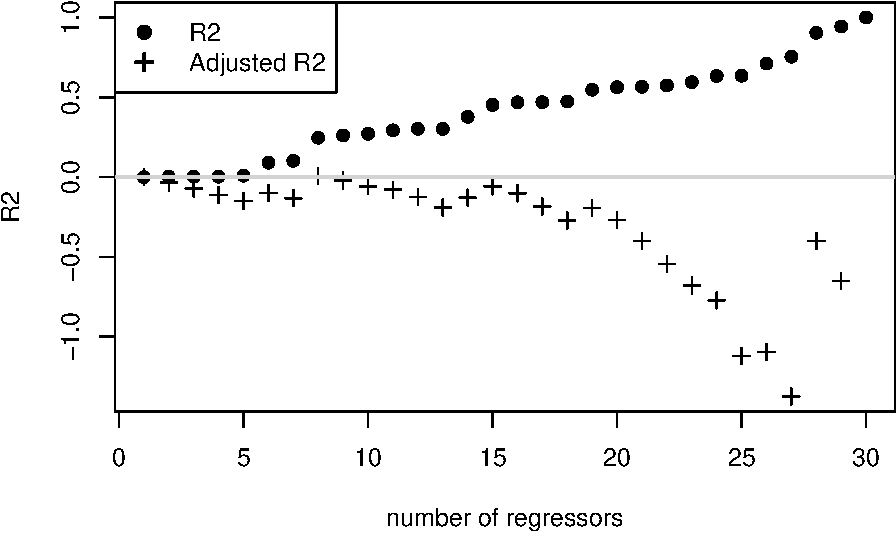
\includegraphics[width=0.9\linewidth]{EcoStat_files/figure-latex/R2issue-1} \caption{This figure illustrates the monotonous increase in the $R^2$ as a function of the number of explanatory variables. In the true model, there is no explanatory variables, i.e., $y_i = \varepsilon_i$. We then take (independent) regressors and regress $y$ on the latter, progressively increasing the set of regressors.}\label{fig:R2issue}
\end{figure}

In order to address the risk of adding irrelevant explanatory variables, measures of \textbf{adjusted \(R^2\)} have been proposed. Compared to the standard \(R^2\), these measures add penalties that depend on the number of covariates employed in the regression. A common adjusted \(R^2\) measure, denoted by \(\bar{R}^2\), is the following:
\begin{equation*}
\boxed{\bar{R}^2 = 1 - \frac{\mathbf{e}'\mathbf{e}/(n-K)}{\mathbf{y}'\mathbf{M}^0\mathbf{y}/(n-1)} = 1 - \frac{n-1}{n-K}(1-R^2).}
\end{equation*}

\hypertarget{inference-and-confidence-intervals-in-small-sample}{%
\subsection{Inference and confidence intervals (in small sample)}\label{inference-and-confidence-intervals-in-small-sample}}

Under the normality assumption (Assumption \ref{hyp:normality}), we know the distribution of \(\mathbf{b}\) (conditional on \(\mathbf{X}\)). Indeed, \(\mathbf{b} = \boldsymbol\beta + (\mathbf{X}'\mathbf{X})^{-1} \mathbf{X}'\boldsymbol\varepsilon\). Therefore, conditional on \(\mathbf{X}\), vector \(\mathbf{b}\) is an affine combination of Gaussian variables---the components of \(\boldsymbol\varepsilon\). As a result, it is also Gaussian. Its distribution is therefore completely characterized by its mean and variance, and we have:
\begin{equation}
\mathbf{b}|\mathbf{X} \sim \mathcal{N}(\boldsymbol\beta,\sigma^2(\mathbf{X}'\mathbf{X})^{-1}).\label{eq:distriBcondi}
\end{equation}

Eq. \eqref{eq:distriBcondi} can be used to conduct inference and tests. However, in practice, we do not know \(\sigma^2\) (which is a population parameter). The following proposition gives an unbiased estimate of \(\sigma^2\).

\begin{proposition}
\protect\hypertarget{prp:expects2}{}\label{prp:expects2}Under \ref{hyp:fullrank} to \ref{hyp:noncorrelResid}, an unbiased estimate of \(\sigma^2\) is given by:
\begin{equation}
s^2 = \frac{\mathbf{e}'\mathbf{e}}{n-K}.\label{eq:s2}
\end{equation}
(It is sometimes denoted by \(\sigma^2_{OLS}\).)
\end{proposition}

\begin{proof}
We have:
\begin{eqnarray*}
\mathbb{E}(\mathbf{e}'\mathbf{e}|\mathbf{X})&=&\mathbb{E}(\boldsymbol{\varepsilon}'\mathbf{M}\boldsymbol{\varepsilon}|\mathbf{X})=\mathbb{E}(\mbox{Tr}(\boldsymbol{\varepsilon}'\mathbf{M}\boldsymbol{\varepsilon})|\mathbf{X}))\\
&=&\mbox{Tr}(\mathbf{M}\mathbb{E}(\boldsymbol{\varepsilon}\boldsymbol{\varepsilon}'|\mathbf{X}))=\sigma^2 \mbox{Tr}(\mathbf{M}).
\end{eqnarray*}
(Note that we have \(\mathbb{E}(\boldsymbol{\varepsilon}\boldsymbol{\varepsilon}'|\mathbf{X})=\sigma^2Id\) by Assumptions \ref{hyp:homoskedasticity} and \ref{hyp:noncorrelResid}, see Prop. \ref{prp:Sigma}.) Moreover:
\begin{eqnarray*}
\mbox{Tr}(\mathbf{M})&=&n-\mbox{Tr}(\mathbf{X}(\mathbf{X}'\mathbf{X})^{-1}\mathbf{X}')\\
&=&n-\mbox{Tr}((\mathbf{X}'\mathbf{X})^{-1}\mathbf{X}'\mathbf{X})=n-\mbox{Tr}(Id_{K \times K}),
\end{eqnarray*}
which leads to the result.
\end{proof}

Two results will prove important to produce inference:

\begin{enumerate}
\def\labelenumi{\roman{enumi}.}
\tightlist
\item
  We know the conditional distribution of \(s^2\) (Prop. \ref{prp:s2distri}).
\item
  \(s^2\) and \(\mathbf{b}\) are independent random variables (Prop. \ref{prp:indeps2b}).
\end{enumerate}

\begin{proposition}
\protect\hypertarget{prp:s2distri}{}\label{prp:s2distri}Under \ref{hyp:fullrank} to \ref{hyp:normality}, we have: \(\dfrac{s^2}{\sigma^2} | \mathbf{X} \sim \frac{1}{n-K}\chi^2(n-K)\).
\end{proposition}

\begin{proof}
We have \(\mathbf{e}'\mathbf{e}=\boldsymbol\varepsilon'\mathbf{M}\boldsymbol\varepsilon\). \(\mathbf{M}\) is an idempotent symmetric matrix. Therefore it can be decomposed as \(PDP'\) where \(D\) is a diagonal matrix and \(P\) is an orthogonal matrix. As a result \(\mathbf{e}'\mathbf{e} = (P'\boldsymbol\varepsilon)'D(P'\boldsymbol\varepsilon)\), i.e.~\(\mathbf{e}'\mathbf{e}\) is a weighted sum of independent squared Gaussian variables (the entries of \(P'\boldsymbol\varepsilon\) are independent because they are Gaussian ---under \ref{hyp:normality}--- and uncorrelated). The variance of each of these i.i.d. Gaussian variable is \(\sigma^2\). Because \(\mathbf{M}\) is an idempotent symmetric matrix, its eigenvalues are either 0 or 1, and its rank equals its trace (see Propositions \ref{prp:rootsidempotent} and \ref{prp:chi2idempotent}). Further, its trace is equal to \(n-K\) (see proof of Eq. \eqref{eq:s2}). Therefore \(D\) has \(n-K\) entries equal to 1 and \(K\) equal to 0. Hence, \(\mathbf{e}'\mathbf{e} = (P'\boldsymbol\varepsilon)'D(P'\boldsymbol\varepsilon)\) is a sum of \(n-K\) squared independent Gaussian variables of variance \(\sigma^2\). Therefore \(\frac{\mathbf{e}'\mathbf{e}}{\sigma^2} = (n-K)\frac{s^2}{\sigma^2}\) is a sum of \(n-k\) squared i.i.d. standard normal variables. The result follows by the definition of the chi-square distribution (see Def. \ref{def:chi2}).
\end{proof}

\begin{proposition}
\protect\hypertarget{prp:indeps2b}{}\label{prp:indeps2b}Under Hypotheses \ref{hyp:fullrank} to \ref{hyp:normality}, \(\mathbf{b}\) and \(s^2\) are independent.
\end{proposition}

\begin{proof}
We have \(\mathbf{b}=\boldsymbol\beta + [\mathbf{X}'{\mathbf{X}}]^{-1}\mathbf{X}\boldsymbol\varepsilon\) and \(s^2 = \boldsymbol\varepsilon' \mathbf{M} \boldsymbol\varepsilon/(n-K)\). Hence \(\mathbf{b}\) is an affine combination of \(\boldsymbol\varepsilon\) and \(s^2\) is a quadratic combination of the same Gaussian shocks. One can write \(s^2\) as \(s^2 = (\mathbf{M}\boldsymbol\varepsilon)' \mathbf{M} \boldsymbol\varepsilon/(n-K)\) and \(\mathbf{b}\) as \(\boldsymbol\beta + \mathbf{T}\boldsymbol\varepsilon\). Since \(\mathbf{T}\mathbf{M}=0\), \(\mathbf{T}\boldsymbol\varepsilon\) and \(\mathbf{M}\boldsymbol\varepsilon\) are independent (because two uncorrelated Gaussian variables are independent), therefore \(\mathbf{b}\) and \(s^2\), which are functions of two sets of independent variables, are independent.
\end{proof}

Consistently with Eq. \eqref{eq:distriBcondi}, under Hypotheses \ref{hyp:fullrank} to \ref{hyp:normality}, the \(k^{th}\) entry of \(\mathbf{b}\) satisfies:
\[
b_k | \mathbf{X} \sim \mathcal{N}(\beta_k,\sigma^2 v_k),
\]
where \(v_k\) is the k\(^{th}\) component of the diagonal of \((\mathbf{X}'\mathbf{X})^{-1}\).

Moreover, we have (Prop. \ref{prp:s2distri}):
\[
\frac{(n-K)s^2}{\sigma^2} | \mathbf{X} \sim \chi ^2 (n-K).
\]

As a result (using Propositions \ref{prp:s2distri} and \ref{prp:indeps2b}), we have:
\begin{equation}
\boxed{t_k = \frac{\frac{b_k - \beta_k}{\sqrt{\sigma^2 v_k}}}{\sqrt{\frac{(n-K)s^2}{\sigma^2(n-K)}}} = \frac{b_k - \beta_k}{\sqrt{s^2v_k}} \sim t(n-K),}\label{eq:resultstudentt}
\end{equation}
where \(t(n-K)\) denotes a Student \(t\) distribution with \(n-K\) degrees of freedom (see Def. \ref{def:tStudent}).\footnote{We have \(\frac{b_k - \beta_k}{\sqrt{\sigma^2 v_k}} | \mathbf{X} \sim \mathcal{N}(0,1)\) and \(\frac{(n-K)s^2}{\sigma^2} | \mathbf{X} \sim \chi ^2 (n-K)\). These two distributions do not depend on \(\mathbf{X}\) \(\Rightarrow\) the \emph{marginal distribution} of \(t_k\) is also \(t\).}

Note that \(s^2 v_k\) is not exactly the conditional variance of \(b_k\): The variance of \(b_k\) conditional on \(\mathbf{X}\) is \(\sigma^2 v_k\). However \(s^2 v_k\) is an unbiased estimate of \(\sigma^2 v_k\) (by Prop. \ref{prp:expects2}).

The previous result (Eq. \eqref{eq:resultstudentt}) can be extended to any linear combinations of elements of \(\mathbf{b}\). (Eq. \eqref{eq:resultstudentt} is for its \(k^{th}\) component only.) Let us consider \(\boldsymbol\alpha'\mathbf{b}\), the OLS estimate of \(\boldsymbol\alpha'\boldsymbol\beta\). From Eq. \eqref{eq:distriBcondi}, we have:
\[
\boldsymbol\alpha'\mathbf{b} | \mathbf{X} \sim \mathcal{N}(\boldsymbol\alpha'\boldsymbol\beta,\sigma^2 \boldsymbol\alpha'(\mathbf{X}'\mathbf{X})^{-1}\boldsymbol\alpha).
\]
Therefore:
\[
\frac{\boldsymbol\alpha'\mathbf{b} - \boldsymbol\alpha'\boldsymbol\beta}{\sqrt{\sigma^2 \boldsymbol\alpha'(\mathbf{X}'\mathbf{X})^{-1}\boldsymbol\alpha}} | \mathbf{X} \sim \mathcal{N}(0,1).
\]
Using the same approach as the one used to derive Eq. \eqref{eq:resultstudentt}, one can show that Props. \ref{prp:s2distri} and \ref{prp:indeps2b} also imply that:
\begin{equation}
\boxed{\frac{\boldsymbol\alpha'\mathbf{b} - \boldsymbol\alpha'\boldsymbol\beta}{\sqrt{s^2\boldsymbol\alpha'(\mathbf{X}'\mathbf{X})^{-1}\boldsymbol\alpha}} \sim t(n-K).}\label{eq:resultstudentt2}
\end{equation}

\begin{figure}
\centering
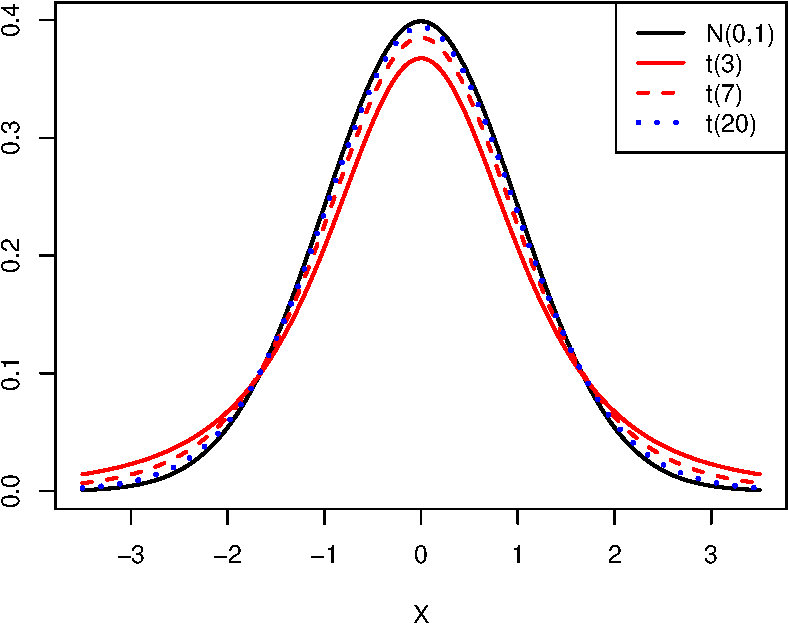
\includegraphics{EcoStat_files/figure-latex/chartStudent-1.pdf}
\caption{\label{fig:chartStudent}The higher the degree of freedom, the closer the distribution of \(t(\nu)\) gets to the normal distribution. (Convergence in distribution.)}
\end{figure}

What precedes is widely exploited for statistical inference in the context of linear regressions. Indeed, Eq. \eqref{eq:resultstudentt} gives a sense of the distances between \(b_k\) and \(\beta_k\) that can be deemed as ``likely'' (or, conversely, ``unlikely''). For instance, it implies that, if \(\sqrt{v_k s^2}\) is equal to 1 (say), then the probability to obtain \(b_k\) smaller than \(\beta_k-\) 4.587 \(\times \sqrt{v_k s^2}\) or larger than \(\beta_k+\) 4.587 \(\times \sqrt{v_k s^2}\) is equal to 0.1\% when \(n-K=10\).

That means for instance that, under the assumption that \(\beta_k=0\), it would be extremely unlikely to have obtained \(b_k/\sqrt{v_k s^2}\) smaller than -4.587 or larger than 4.587. More generally, this shows that the \textbf{t-statistic}, i.e., the ratio \(b_k/\sqrt{v_k s^2}\), is the test statistic associated with the null hypothesis:
\[
H_0: \beta_k=0.
\]
Under the null hypothesis, the test statistic follows a Student-t distribution with \(n-K\) degrees of freedom. The \textbf{t-statistic} is therefore of particular importance, and, as a result, it is routinely reported in regression outputs (see Example \ref{exm:SHP0001}).

\begin{example}[Education and income]
\protect\hypertarget{exm:SHP0001}{}\label{exm:SHP0001}

Consider regression that aims at determining covariates of households' income. This example makes use of data from the \href{https://forscenter.ch/projects/swiss-household-panel/}{Swiss Household Panel (SHP)}; \texttt{edyear19} is the number of years of education and \texttt{age19} is the age of the respondent, as of 2019.

\begin{Shaded}
\begin{Highlighting}[]
\FunctionTok{library}\NormalTok{(AEC)}
\FunctionTok{library}\NormalTok{(sandwich)}
\NormalTok{shp}\SpecialCharTok{$}\NormalTok{income }\OtherTok{\textless{}{-}}\NormalTok{ shp}\SpecialCharTok{$}\NormalTok{i19ptotn}\SpecialCharTok{/}\DecValTok{1000}
\NormalTok{shp}\SpecialCharTok{$}\NormalTok{female }\OtherTok{\textless{}{-}} \DecValTok{1}\SpecialCharTok{*}\NormalTok{(shp}\SpecialCharTok{$}\NormalTok{sex19}\SpecialCharTok{==}\DecValTok{2}\NormalTok{)}
\NormalTok{eq }\OtherTok{\textless{}{-}} \FunctionTok{lm}\NormalTok{(income }\SpecialCharTok{\textasciitilde{}}\NormalTok{ edyear19 }\SpecialCharTok{+}\NormalTok{ age19 }\SpecialCharTok{+} \FunctionTok{I}\NormalTok{(age19}\SpecialCharTok{\^{}}\DecValTok{2}\NormalTok{) }\SpecialCharTok{+}\NormalTok{ female,}\AttributeTok{data=}\NormalTok{shp)}
\NormalTok{lmtest}\SpecialCharTok{::}\FunctionTok{coeftest}\NormalTok{(eq)}
\end{Highlighting}
\end{Shaded}

\begin{verbatim}
## 
## t test of coefficients:
## 
##                Estimate  Std. Error t value  Pr(>|t|)    
## (Intercept) -71.9738073   5.7082456 -12.609 < 2.2e-16 ***
## edyear19      4.8442661   0.2172320  22.300 < 2.2e-16 ***
## age19         3.2386215   0.2183812  14.830 < 2.2e-16 ***
## I(age19^2)   -0.0289498   0.0020915 -13.842 < 2.2e-16 ***
## female      -31.8089006   1.4578004 -21.820 < 2.2e-16 ***
## ---
## Signif. codes:  0 '***' 0.001 '**' 0.01 '*' 0.05 '.' 0.1 ' ' 1
\end{verbatim}

\end{example}

The last two columns of the previous table give the t-statistic and the p-values associated with t-tests, whose size-\(\alpha\) critical region is:
\[
\left]-\infty,-\Phi^{-1}_{t(n-K)}\left(1-\frac{\alpha}{2}\right)\right] \cup \left[\Phi^{-1}_{t(n-K)}\left(1-\frac{\alpha}{2}\right),+\infty\right[.
\]

We recall that the \textbf{p-value} is defined as the probability that \(|Z| > |t|\), where \(t\) is the (computed) t-statistics and where \(Z \sim t(n-K)\). That is, in the context of the t-test, the p-value is given by \(2(1 - \Phi_{t(n-K)}(|t_k|))\). See \href{https://jrenne.shinyapps.io/tests/}{this webpage} for details regarding the link between critical regions, p-value, and test outcomes.

Now, suppose we want to compute a (symmetrical) \emph{confidence interval} \([I_{d,1-\alpha},I_{u,1-\alpha}]\) that is such that \(\mathbb{P}(\beta_k \in [I_{d,1-\alpha},I_{u,1-\alpha}])=1-\alpha\). That is, we want to have: \(\mathbb{P}(\beta_k < I_{d,1-\alpha})=\frac{\alpha}{2}\) and \(\mathbb{P}(\beta_k > I_{u,1-\alpha})=\frac{\alpha}{2}\). Let us focus on \(I_{d,1-\alpha}\) to start with. Using Eq. \eqref{eq:resultstudentt}, i.e., \(t_k = \frac{b_k - \beta_k}{\sqrt{s^2v_k}} \sim t(n-K)\), we have:
\begin{eqnarray*}
\mathbb{P}(\beta_k < I_{d,1-\alpha})=\frac{\alpha}{2} &\Leftrightarrow& \\
\mathbb{P}\left(\frac{b_k - \beta_k}{\sqrt{s^2v_k}} > \frac{b_k - I_{d,1-\alpha}}{\sqrt{s^2v_k}}\right)=\frac{\alpha}{2} &\Leftrightarrow& \mathbb{P}\left(t_k > \frac{b_k - I_{d,1-\alpha}}{\sqrt{s^2v_k}}\right)=\frac{\alpha}{2} \Leftrightarrow\\
1 - \mathbb{P}\left(t_k \le \frac{b_k - I_{d,1-\alpha}}{\sqrt{s^2v_k}}\right)=\frac{\alpha}{2} &\Leftrightarrow& \frac{b_k - I_{d,1-\alpha}}{\sqrt{s^2v_k}} = \Phi^{-1}_{t(n-K)}\left(1-\frac{\alpha}{2}\right),
\end{eqnarray*}
where \(\Phi_{t(n-K)}(\alpha)\) is the c.d.f. of the \(t(n-K)\) distribution (Table \ref{tab:Student}).

Doing the same for \(I_{u,1-\alpha}\), we obtain:
\begin{eqnarray*}
&&[I_{d,1-\alpha},I_{u,1-\alpha}] =\\
&&\left[b_k - \Phi^{-1}_{t(n-K)}\left(1-\frac{\alpha}{2}\right)\sqrt{s^2v_k},b_k + \Phi^{-1}_{t(n-K)}\left(1-\frac{\alpha}{2}\right)\sqrt{s^2v_k}\right].
\end{eqnarray*}

Using the results presented in Example \ref{exm:SHP0001}, we can compute lower and upper bounds of 95\% confidence intervals for the estimated parameters as follows:

\begin{Shaded}
\begin{Highlighting}[]
\NormalTok{n }\OtherTok{\textless{}{-}} \FunctionTok{length}\NormalTok{(eq}\SpecialCharTok{$}\NormalTok{residuals); K }\OtherTok{\textless{}{-}} \FunctionTok{length}\NormalTok{(eq}\SpecialCharTok{$}\NormalTok{coefficients)}
\NormalTok{lower.b }\OtherTok{\textless{}{-}}\NormalTok{ eq}\SpecialCharTok{$}\NormalTok{coefficients }\SpecialCharTok{+} \FunctionTok{qt}\NormalTok{(.}\DecValTok{025}\NormalTok{,}\AttributeTok{df=}\NormalTok{n}\SpecialCharTok{{-}}\NormalTok{K)}\SpecialCharTok{*}\FunctionTok{sqrt}\NormalTok{(}\FunctionTok{diag}\NormalTok{(}\FunctionTok{vcov}\NormalTok{(eq)))}
\NormalTok{upper.b }\OtherTok{\textless{}{-}}\NormalTok{ eq}\SpecialCharTok{$}\NormalTok{coefficients }\SpecialCharTok{+} \FunctionTok{qt}\NormalTok{(.}\DecValTok{975}\NormalTok{,}\AttributeTok{df=}\NormalTok{n}\SpecialCharTok{{-}}\NormalTok{K)}\SpecialCharTok{*}\FunctionTok{sqrt}\NormalTok{(}\FunctionTok{diag}\NormalTok{(}\FunctionTok{vcov}\NormalTok{(eq)))}
\FunctionTok{cbind}\NormalTok{(lower.b,upper.b)}
\end{Highlighting}
\end{Shaded}

\begin{verbatim}
##                  lower.b      upper.b
## (Intercept) -83.16413225 -60.78348237
## edyear19      4.41840914   5.27012310
## age19         2.81051152   3.66673148
## I(age19^2)   -0.03304986  -0.02484977
## female      -34.66674188 -28.95105932
\end{verbatim}

\hypertarget{Ftest}{%
\subsection{Testing a set of linear restrictions}\label{Ftest}}

We sometimes want to test if a set of restrictions are \emph{jointly} consistent with the data at hand. Let us formalize such a set of (\(J\)) linear restrictions:
\begin{equation}\label{eq:restrictions}
\begin{array}{ccc}
r_{1,1} \beta_1 + \dots + r_{1,K} \beta_K &=& q_1\\
\vdots && \vdots\\
r_{J,1} \beta_1 + \dots + r_{J,K} \beta_K &=& q_J.
\end{array}
\end{equation}
In matrix form, we get:
\begin{equation}
\mathbf{R}\boldsymbol\beta = \mathbf{q}.
\end{equation}

Define the \emph{discrepancy vector} \(\mathbf{m} = \mathbf{R}\mathbf{b} - \mathbf{q}\). Under the null hypothesis:
\begin{eqnarray*}
\mathbb{E}(\mathbf{m}|\mathbf{X}) &=& \mathbf{R}\boldsymbol\beta - \mathbf{q} = 0 \quad \mbox{and} \\
\mathbb{V}ar(\mathbf{m}|\mathbf{X}) &=& \mathbf{R} \mathbb{V}ar(\mathbf{b}|\mathbf{X}) \mathbf{R}'.
\end{eqnarray*}

With these notations, the assumption to test is:
\begin{equation}
\boxed{H_0: \mathbf{R}\boldsymbol\beta - \mathbf{q} = 0 \mbox{ against } H_1: \mathbf{R}\boldsymbol\beta - \mathbf{q} \ne 0.}\label{eq:H0Ftest}
\end{equation}

Under Hypotheses \ref{hyp:fullrank} to \ref{hyp:noncorrelResid}, we have \(\mathbb{V}ar(\mathbf{m}|\mathbf{X}) = \sigma^2 \mathbf{R} (\mathbf{X}'\mathbf{X})^{-1} \mathbf{R}'\) (see Prop. \ref{prp:propOLS}). If we add the normality assumption (Hypothesis \ref{hyp:normality}), we have:
\begin{equation}
W = \mathbf{m}'\mathbb{V}ar(\mathbf{m}|\mathbf{X})^{-1}\mathbf{m} \sim \chi^2(J). \label{eq:W1}
\end{equation}

If \(\sigma^2\) was known, we could then conduct a \emph{Wald test} (directly exploiting Eq. \eqref{eq:W1}). But this is not the case in practice and we cannot compute \(W\). We can, however, approximate it be replacing \(\sigma^2\) by \(s^2\) (given in Eq. \eqref{eq:s2}). The distribution of this new statistic is not \(\chi^2(J)\) any more; it is an \emph{\(\mathcal{F}\) distribution} (whose quantiles are shown in Table \ref{tab:Fstat}), and the test is called \emph{\(F\) test}.

\begin{proposition}
\protect\hypertarget{prp:Ftest1}{}\label{prp:Ftest1}Under Hypotheses \ref{hyp:fullrank} to \ref{hyp:normality} and if Eq. \eqref{eq:H0Ftest} holds, we have:
\begin{equation}
F = \frac{W}{J}\frac{\sigma^2}{s^2} = \frac{\mathbf{m}'(\mathbf{R}(\mathbf{X}'\mathbf{X})^{-1}\mathbf{R}')^{-1}\mathbf{m}}{s^2J} \sim \mathcal{F}(J,n-K),\label{eq:defFstatistics}
\end{equation}
where \(\mathcal{F}\) is the distribution of the F-statistic (see Def. \ref{def:fstatistics}).
\end{proposition}

\begin{proof}
According to Eq. \eqref{eq:W1}, \(W/J \sim \chi^2(J)/J\). Moreover, the denominator (\(s^2/\sigma^2\)) is \(\sim \chi^2(n-K)\). Therefore, \(F\) is the ratio of a r.v. distributed as \(\chi^2(J)/J\) and another distributed as \(\chi^2(n-K)/(n-K)\). It remains to verify that these r.v. are independent. Under \(H_0\), we have \(\mathbf{m} = \mathbf{R}(\mathbf{b}-\boldsymbol\beta) = \mathbf{R}(\mathbf{X}'\mathbf{X})^{-1}\mathbf{X}'\boldsymbol\varepsilon\).
Therefore \(\mathbf{m}'(\mathbf{R}(\mathbf{X}'\mathbf{X})^{-1}\mathbf{R}')^{-1}\mathbf{m}\) is of the form \(\boldsymbol\varepsilon'\mathbf{T}\boldsymbol\varepsilon\) with \(\mathbf{T}=\mathbf{D}'\mathbf{C}\mathbf{D}\) where \(\mathbf{D}=\mathbf{R}(\mathbf{X}'\mathbf{X})^{-1}\mathbf{X}'\) and \(\mathbf{C}=(\mathbf{R}(\mathbf{X}'\mathbf{X})^{-1}\mathbf{R}')^{-1}\). Under Hypotheses \ref{hyp:fullrank} to \ref{hyp:noncorrelResid}, the covariance between \(\mathbf{T}\boldsymbol\varepsilon\) and \(\mathbf{M}\boldsymbol\varepsilon\) is \(\sigma^2\mathbf{T}\mathbf{M} = \mathbf{0}\). Therefore, under \ref{hyp:normality}, these variables are Gaussian variables with 0 covariance. Hence they are independent.
\end{proof}

For large \(n-K\), the \(\mathcal{F}_{J,n-K}\) distribution converges to \(\mathcal{F}_{J,\infty}=\chi^2(J)/J\). This implies that, in large samples, the F-statistic approximately has a \(\chi^2\) distribution. In other words, one can approximately employ Eq. \eqref{eq:W1} to perform a Wald test (one just has to replace \(\sigma^2\) with \(s^2\) when computing \(\mathbb{V}ar(\mathbf{m}|\mathbf{X})\)).

The following proposition proposes another equivalent computation of the F-statistic, based on the \(R^2\) of the restricted and unrestricted linear models.

\begin{proposition}
\protect\hypertarget{prp:Ftest}{}\label{prp:Ftest}The F-statistic defined by Eq. \eqref{eq:defFstatistics} is also equal to:
\begin{equation}
F = \frac{(R^2-R_*^2)/J}{(1-R^2)/(n-K)} =  \frac{(SSR_{restr}-SSR_{unrestr})/J}{SSR_{unrestr}/(n-K)},\label{eq:defFstatistics2}
\end{equation}
where \(R_*^2\) is the coef. of determination (Eq. \eqref{eq:RR2}) of the ``restricted regression'' \emph{(SSR: sum of squared residuals.)}
\end{proposition}

\begin{proof}
Let's denote by \(\mathbf{e}_*=\mathbf{y}-\mathbf{X}\mathbf{b}_*\) the vector of residuals associated to the \emph{restricted regression} (i.e.~\(\mathbf{R}\mathbf{b}_*=\mathbf{q}\)).
We have \(\mathbf{e}_*=\mathbf{e} - \mathbf{X}(\mathbf{b}_*-\mathbf{b})\). Using \(\mathbf{e}'\mathbf{X}=0\), we get \(\mathbf{e}_*'\mathbf{e}_*=\mathbf{e}'\mathbf{e} + (\mathbf{b}_*-\mathbf{b})'\mathbf{X}'\mathbf{X}(\mathbf{b}_*-\mathbf{b}) \ge \mathbf{e}'\mathbf{e}\).

By Proposition \ref{prp:constrainedLS} (in Appendix \ref{LinAlgebra}), we have: \(\mathbf{b}_*-\mathbf{b}=-(\mathbf{X}'\mathbf{X})^{-1} \mathbf{R}'\{\mathbf{R}(\mathbf{X}'\mathbf{X})^{-1}\mathbf{R}'\}^{-1}(\mathbf{R}\mathbf{b} - \mathbf{q})\). Therefore:
\[
\mathbf{e}_*'\mathbf{e}_* - \mathbf{e}'\mathbf{e} = (\mathbf{R}\mathbf{b} - \mathbf{q})'[\mathbf{R}(\mathbf{X}'\mathbf{X})^{-1}\mathbf{R}']^{-1}(\mathbf{R}\mathbf{b} - \mathbf{q}).
\]
This implies that the F statistic defined in Prop. \ref{prp:Ftest1} is also equal to:
\[
\frac{(\mathbf{e}_*'\mathbf{e}_* - \mathbf{e}'\mathbf{e})/J}{\mathbf{e}'\mathbf{e}/(n-K)},
\]
which leads to the result.
\end{proof}

The null hypothesis \(H_0\) (Eq. \eqref{eq:H0Ftest}) of the F-test is rejected if \(F\) ---defined by Eq. \eqref{eq:defFstatistics} or \eqref{eq:defFstatistics2}--- is higher than \(\mathcal{F}_{1-\alpha}(J,n-K)\). (Hence, this test is a one-sided test.)

\hypertarget{largeSample}{%
\subsection{Large Sample Properties}\label{largeSample}}

Even if we relax the normality assumption (Hypothesis \ref{hyp:normality}), we can approximate the finite-sample behavior of the estimators by using \emph{large-sample} or \emph{asymptotic properties}.

To begin with, we proceed under Hypothesis \ref{hyp:fullrank} to \ref{hyp:noncorrelResid}. (We will see, later on, how to deal with ---partial--- relaxations of Hypothesis \ref{hyp:homoskedasticity} and \ref{hyp:noncorrelResid}.)

Under regularity assumptions, and under Hypotheses \ref{hyp:fullrank} to \ref{hyp:noncorrelResid}, even if the residuals are not normally-distributed, the least square estimators can be \emph{asymptotically normal} and inference can be performed in the same way as in small samples when Hypotheses \ref{hyp:fullrank} to \ref{hyp:normality} hold. This derives from Prop. \ref{prp:asymptOLS} (below). The F-test (Prop. \ref{prp:Ftest}) and the t-test (Eq. \eqref{eq:resultstudentt}) can then be performed.

\begin{proposition}
\protect\hypertarget{prp:asymptOLS}{}\label{prp:asymptOLS}Under Assumptions \ref{hyp:fullrank} to \ref{hyp:noncorrelResid}, and assuming further that:
\begin{equation}
Q = \mbox{plim}_{n \rightarrow \infty} \frac{\mathbf{X}'\mathbf{X}}{n},\label{eq:Qasympt}
\end{equation}
and that the \((\mathbf{x}_i,\varepsilon_i)\)'s are independent (across entities \(i\)), we have:
\begin{equation}
\sqrt{n}(\mathbf{b} - \boldsymbol\beta)\overset{d} {\rightarrow} \mathcal{N}\left(0,\sigma^2Q^{-1}\right).\label{eq:convgceOLS}
\end{equation}
\end{proposition}

\begin{proof}
Since \(\mathbf{b} = \boldsymbol\beta + \left( \frac{\mathbf{X}'\mathbf{X}}{n}\right)^{-1}\left(\frac{\mathbf{X}'\boldsymbol\varepsilon}{n}\right)\), we have: \(\sqrt{n}(\mathbf{b} - \boldsymbol\beta) = \left( \frac{\mathbf{X}'\mathbf{X}}{n}\right)^{-1} \left(\frac{1}{\sqrt{n}}\right)\mathbf{X}'\boldsymbol\varepsilon\). Since \(f:A \rightarrow A^{-1}\) is a continuous function (for \(A \ne \mathbf{0}\)), \(\mbox{plim}_{n \rightarrow \infty} \left(\frac{\mathbf{X}'\mathbf{X}}{n}\right)^{-1} = \mathbf{Q}^{-1}\) (see Prop. \ref{prp:Slutsky}). Let us denote by \(V_i\) the vector \(\mathbf{x}_i \varepsilon_i\). Because the \((\mathbf{x}_i,\varepsilon_i)\)'s are independent, the \(V_i\)'s are independent as well. Their covariance matrix is \(\sigma^2\mathbb{E}(\mathbf{x}_i \mathbf{x}_i')=\sigma^2Q\). Applying the multivariate central limit theorem on vectors \(V_i\) gives \(\sqrt{n}\left(\frac{1}{n}\sum_{i=1}^n \mathbf{x}_i \varepsilon_i\right) = \left(\frac{1}{\sqrt{n}}\right)\mathbf{X}'\boldsymbol\varepsilon \overset{d}{\rightarrow} \mathcal{N}(0,\sigma^2Q)\). An application of Slutsky's theorem (Prop. \ref{prp:Slutsky}) then leads to the results.
\end{proof}

In practice, \(\sigma^2\) is approximated by \(s^2=\frac{\mathbf{e}'\mathbf{e}}{n-K}\) (Eq. \eqref{eq:s2}) and \(\mathbf{Q}^{-1}\) by \(\left(\frac{\mathbf{X}'\mathbf{X}}{n}\right)^{-1}\). That is, the covariance matrix of the estimator is approximated by:
\begin{equation}
\boxed{\widehat{\mathbb{V}ar}(\mathbf{b}) = s^2 (\mathbf{X}'\mathbf{X})^{-1}.}\label{eq:sXX}
\end{equation}

Eqs. \eqref{eq:Qasympt} and \eqref{eq:convgceOLS} respectively correspond to convergences in probability and in distribution (see Definitions \ref{def:convergenceproba} and \ref{def:cvgceDistri}, respectively).

\hypertarget{CommonPitfalls}{%
\section{Common pitfalls in linear regressions}\label{CommonPitfalls}}

\hypertarget{multicollinearity}{%
\subsection{Multicollinearity}\label{multicollinearity}}

Consider the model: \(y_i = \beta_1 x_{i,1} + \beta_2 x_{i,2} + \varepsilon_i\), where all variables are zero-mean and \(\mathbb{V}ar(\varepsilon_i)=\sigma^2\). We have:
\[
\mathbf{X}'\mathbf{X} = \left[ \begin{array}{cc}
\sum_i x_{i,1}^2 & \sum_i x_{i,1} x_{i,2} \\
\sum_i x_{i,1} x_{i,2} & \sum_i x_{i,2}^2
\end{array}\right],
\]
therefore:
\begin{eqnarray*}
(\mathbf{X}'\mathbf{X})^{-1} &=& \frac{1}{\sum_i x_{i,1}^2\sum_i x_{i,2}^2 - (\sum_i x_{i,1} x_{i,2})^2} \left[ \begin{array}{cc}
\sum_i x_{i,2}^2 & -\sum_i x_{i,1} x_{i,2} \\
-\sum_i x_{i,1} x_{i,2} & \sum_i x_{i,1}^2
\end{array}\right].
\end{eqnarray*}
The inverse of the upper-left parameter of \((\mathbf{X}'\mathbf{X})^{-1}\) is:
\begin{equation}
\sum_i x_{i,1}^2 - \frac{(\sum_i x_{i,1} x_{i,2})^2}{\sum_i x_{i,2}^2} = \sum_i x_{i,1}^2(1 - correl_{1,2}^2),\label{eq:multicollin}
\end{equation}
where \(correl_{1,2}\) is the sample correlation between \(\mathbf{x}_{1}\) and \(\mathbf{x}_{2}\).

Hence, the closer to one \(correl_{1,2}\), the higher the variance of \(b_1\) (recall that the variance of \(b_1\) is the upper-left component of \(\sigma^2(\mathbf{X}'\mathbf{X})^{-1}\)). That is, if some of our regressors are close to a linear conbination of the other ones, then the confidence intervals will tend to be wide, which typically reduces the power of the t-test (we tend to fail to reject the null hypothesis that the coefficients are different from zero).

\hypertarget{Omitted}{%
\subsection{Omitted variables}\label{Omitted}}

Consider the following model (the ``True model''):
\[
\mathbf{y} = \underbrace{\mathbf{X}_1}_{n \times K_1}\underbrace{\boldsymbol\beta_1}_{K_1 \times 1} + \underbrace{\mathbf{X}_2}_{n\times K_2}\underbrace{\boldsymbol\beta_2}_{K_2 \times 1} + \boldsymbol\varepsilon
\]
If one computes \(\mathbf{b}_1\) by regressing \(\mathbf{y}\) on \(\mathbf{X}_1\) only, one gets:
\[
\mathbf{b}_1 = (\mathbf{X}_1'\mathbf{X}_1)^{-1}\mathbf{X}_1'\mathbf{y} = \boldsymbol\beta_1 + (\mathbf{X}_1'\mathbf{X}_1)^{-1}\mathbf{X}_1'\mathbf{X}_2\boldsymbol\beta_2 + 
(\mathbf{X}_1'\mathbf{X}_1)^{-1}\mathbf{X}_1'\boldsymbol\varepsilon.
\]

This results in the omitted-variable formula:
\[
\mathbb{E}(\mathbf{b}_1|\mathbf{X}) = \boldsymbol\beta_1 + \underbrace{(\mathbf{X}_1'\mathbf{X}_1)^{-1}(\mathbf{X}_1'\mathbf{X}_2)}_{K_1 \times K_2}\boldsymbol\beta_2.
\]
(Each column of \((\mathbf{X}_1'\mathbf{X}_1)^{-1}(\mathbf{X}_1'\mathbf{X}_2)\) are the OLS regressors obtained when regressing the columns of \(\mathbf{X}_2\) on \(\mathbf{X}_1\).) Unless the variables included in \(\mathbf{X}_1\) are orthogonal to those in \(\mathbf{X}_2\), we obtain a bias. A way to address this potential pitfall is to introduce ``controls'' in the specification.

\begin{example}
\protect\hypertarget{exm:CASchools}{}\label{exm:CASchools}

Let us use the \href{https://rdrr.io/cran/AER/man/CASchools.html}{California Test Score dataset} (in the package \texttt{AER}). Assume we want to measure the effect of the students-to-teacher ratio (\texttt{str}) on student test scores (\texttt{testscr}). The following regressions show that the effect is lower when controls are added.

\begin{Shaded}
\begin{Highlighting}[]
\FunctionTok{library}\NormalTok{(AER); }\FunctionTok{data}\NormalTok{(}\StringTok{"CASchools"}\NormalTok{)}
\NormalTok{CASchools}\SpecialCharTok{$}\NormalTok{str }\OtherTok{\textless{}{-}}\NormalTok{ CASchools}\SpecialCharTok{$}\NormalTok{students}\SpecialCharTok{/}\NormalTok{CASchools}\SpecialCharTok{$}\NormalTok{teachers}
\NormalTok{CASchools}\SpecialCharTok{$}\NormalTok{testscr }\OtherTok{\textless{}{-}}\NormalTok{ .}\DecValTok{5} \SpecialCharTok{*}\NormalTok{ (CASchools}\SpecialCharTok{$}\NormalTok{math }\SpecialCharTok{+}\NormalTok{ CASchools}\SpecialCharTok{$}\NormalTok{read)}
\NormalTok{eq1 }\OtherTok{\textless{}{-}} \FunctionTok{lm}\NormalTok{(testscr}\SpecialCharTok{\textasciitilde{}}\NormalTok{str,}\AttributeTok{data=}\NormalTok{CASchools)}
\NormalTok{eq2 }\OtherTok{\textless{}{-}} \FunctionTok{lm}\NormalTok{(testscr}\SpecialCharTok{\textasciitilde{}}\NormalTok{str}\SpecialCharTok{+}\NormalTok{lunch,}\AttributeTok{data=}\NormalTok{CASchools)}
\NormalTok{eq3 }\OtherTok{\textless{}{-}} \FunctionTok{lm}\NormalTok{(testscr}\SpecialCharTok{\textasciitilde{}}\NormalTok{str}\SpecialCharTok{+}\NormalTok{lunch}\SpecialCharTok{+}\NormalTok{english,}\AttributeTok{data=}\NormalTok{CASchools)}
\NormalTok{stargazer}\SpecialCharTok{::}\FunctionTok{stargazer}\NormalTok{(eq1,eq2,eq3,}\AttributeTok{type=}\StringTok{"text"}\NormalTok{,}
                     \AttributeTok{no.space =} \ConstantTok{TRUE}\NormalTok{,}\AttributeTok{omit.stat=}\FunctionTok{c}\NormalTok{(}\StringTok{"f"}\NormalTok{,}\StringTok{"ser"}\NormalTok{))}
\end{Highlighting}
\end{Shaded}

\begin{verbatim}
## 
## =============================================
##                    Dependent variable:       
##              --------------------------------
##                          testscr             
##                 (1)        (2)        (3)    
## ---------------------------------------------
## str          -2.280***  -1.117***  -0.998*** 
##               (0.480)    (0.240)    (0.239)  
## lunch                   -0.600***  -0.547*** 
##                          (0.017)    (0.022)  
## english                            -0.122*** 
##                                     (0.032)  
## Constant     698.933*** 702.911*** 700.150***
##               (9.467)    (4.700)    (4.686)  
## ---------------------------------------------
## Observations    420        420        420    
## R2             0.051      0.767      0.775   
## Adjusted R2    0.049      0.766      0.773   
## =============================================
## Note:             *p<0.1; **p<0.05; ***p<0.01
\end{verbatim}

\end{example}

\hypertarget{irrelevant}{%
\subsection{Irrelevant variable}\label{irrelevant}}

Consider the \emph{true model}:
\[
\mathbf{y} = \mathbf{X}_1\boldsymbol\beta_1 + \boldsymbol\varepsilon,
\]
while the \emph{estimated model} is:
\[
\mathbf{y} = \mathbf{X}_1\boldsymbol\beta_1 + \mathbf{X}_2\boldsymbol\beta_2 + \boldsymbol\varepsilon
\]

The estimates are unbiased. However, adding irrelevant explanatory variables increases the variance of the estimate of \(\boldsymbol\beta_1\) (compared to the case where one uses the correct explanatory variables). This is the case unless the correlation between \(\mathbf{X}_1\) and \(\mathbf{X}_2\) is null, see Eq. \eqref{eq:multicollin}.

In other words, the estimator is \emph{inefficient}, i.e., there exists an alternative consistent estimator whose variance is lower. The inefficiency problem can have serious consequences when testing hypotheses such as \(H_0: \beta_1 = 0\). Due to the loss of power, we might wrongly infer that the \(\mathbf{X}_1\) variables are not ``relevant'' (\emph{Type-II error, False Negative}).

\hypertarget{IV}{%
\section{Instrumental Variables}\label{IV}}

The conditional mean zero assumption (Hypothesis \ref{hyp:exogeneity}), according to which \(\mathbb{E}(\boldsymbol\varepsilon|\mathbf{X})=0\) ---which implies in particular that \(\mathbf{x}_i\) and \(\varepsilon_i\) are uncorrelated--- is sometimes not consistent with the considered economic framework. When it is the case, the parameters of interest may still be estimated consistently by resorting to instrumental variable techniques.

Consider the following model:
\begin{equation}
y_i = \mathbf{x_i}'\boldsymbol\beta + \varepsilon_i, \quad \mbox{where } \mathbb{E}(\varepsilon_i)=0  \mbox{ and } \mathbf{x_i}\not\perp \varepsilon_i.\label{eq:modelIV}
\end{equation}

Let us illustrate how this situation may result in biased OLS estimate. Consider for instance the situation where:
\begin{equation}
\mathbb{E}(\varepsilon_i)=0 \quad \mbox{and} \quad \mathbb{E}(\varepsilon_i \mathbf{x_i})=\boldsymbol\gamma,\label{eq:exmIV}
\end{equation}
in which case we have \(\mathbf{x}_i\not\perp \varepsilon_i\) (consistently with Eq. \eqref{eq:modelIV}).

By the law of large numbers, \(\mbox{plim}_{n \rightarrow \infty} \mathbf{X}'\boldsymbol\varepsilon / n = \boldsymbol\gamma\). If \(\mathbf{Q}_{xx} := \mbox{plim } \mathbf{X}'\mathbf{X}/n\), the OLS estimator is not consistent because
\[
\mathbf{b} = \boldsymbol\beta + (\mathbf{X}'\mathbf{X})^{-1}\mathbf{X}'\boldsymbol\varepsilon \overset{p}{\rightarrow} \boldsymbol\beta + \mathbf{Q}_{xx}^{-1}\boldsymbol\gamma \ne \boldsymbol\beta.
\]

Let us now introduce the notion of instruments.

\begin{definition}[Instrumental variables]
\protect\hypertarget{def:instruments}{}\label{def:instruments}

The \(L\)-dimensional random variable \(\mathbf{z}_i\) is a valid set of instruments if:

\begin{enumerate}
\def\labelenumi{\alph{enumi}.}
\tightlist
\item
  \(\mathbf{z}_i\) is correlated to \(\mathbf{x}_i\);
\item
  we have \(\mathbb{E}(\boldsymbol\varepsilon|\mathbf{Z})=0\) and
\item
  the orthogonal projections of the \(\mathbf{x}_i\)'s on the \(\mathbf{z}_i\)'s are not multicollinear.
\end{enumerate}

\end{definition}

Point c implies in particular that the dimension of \(\mathbf{z}_i\) has to be at least as large as that of \(\mathbf{x}_i\). If \(\mathbf{z}_i\) is a valid set of instruments, we have:
\[
\mbox{plim}\left( \frac{\mathbf{Z}'\mathbf{y}}{n} \right) =\mbox{plim}\left( \frac{\mathbf{Z}'(\mathbf{X}\boldsymbol\beta + \boldsymbol\varepsilon)}{n} \right) = \mbox{plim}\left( \frac{\mathbf{Z}'\mathbf{X}}{n} \right)\boldsymbol\beta.
\]
Indeed, by the law of large numbers, \(\frac{\mathbf{Z}'\boldsymbol\varepsilon}{n} \overset{p}{\rightarrow}\mathbb{E}(\mathbf{z}_i\varepsilon_i)=0\).

If \(L = K\), the matrix \(\frac{\mathbf{Z}'\mathbf{X}}{n}\) is of dimension \(K \times K\) and we have:
\[
\left[\mbox{plim }\left( \frac{\mathbf{Z}'\mathbf{X}}{n} \right)\right]^{-1}\mbox{plim }\left( \frac{\mathbf{Z}'\mathbf{y}}{n} \right) = \boldsymbol\beta.
\]
By continuity of the inverse function (everywhere but at 0): \(\left[\mbox{plim }\left( \frac{\mathbf{Z}'\mathbf{X}}{n} \right)\right]^{-1}=\mbox{plim }\left( \frac{\mathbf{Z}'\mathbf{X}}{n} \right)^{-1}\).
The Slutsky Theorem (Prop. \ref{prp:Slutsky}) further implies that:
\[
\mbox{plim }\left( \frac{\mathbf{Z}'\mathbf{X}}{n} \right)^{-1} \mbox{plim }\left( \frac{\mathbf{Z}'\mathbf{y}}{n} \right)  = \mbox{plim }\left( \left( \frac{\mathbf{Z}'\mathbf{X}}{n} \right)^{-1} \frac{\mathbf{Z}'\mathbf{y}}{n} \right).
\]
Hence \(\mathbf{b}_{iv}\) is consistent if it is defined by:
\[
\boxed{\mathbf{b}_{iv} = (\mathbf{Z}'\mathbf{X})^{-1}\mathbf{Z}'\mathbf{y}.}
\]

\begin{proposition}[Asymptotic distribution of the IV estimator]
\protect\hypertarget{prp:IV}{}\label{prp:IV}If \(\mathbf{z}_i\) is a \(L\)-dimensional random variable that constitutes a valid set of instruments (see Def. \ref{def:instruments}) and if \(L=K\), then the asymptotic distribution of \(\mathbf{b}_{iv}\) is:
\[
\mathbf{b}_{iv} \overset{d}{\rightarrow} \mathcal{N}\left(\boldsymbol\beta,\frac{\sigma^2}{n}\left[Q_{xz}Q_{zz}^{-1}Q_{zx}\right]^{-1}\right)
\]
where \(\mbox{plim } \mathbf{Z}'\mathbf{Z}/n =: \mathbf{Q}_{zz}\), \(\mbox{plim } \mathbf{Z}'\mathbf{X}/n =: \mathbf{Q}_{zx}\), \(\mbox{plim } \mathbf{X}'\mathbf{Z}/n =: \mathbf{Q}_{xz}\).
\end{proposition}

\begin{proof}
The proof is very similar to that of Prop. \ref{prp:asymptOLS}, the starting point being that \(\mathbf{b}_{iv} = \boldsymbol\beta + (\mathbf{Z}'\mathbf{X})^{-1}\mathbf{Z}'\boldsymbol\varepsilon\).
\end{proof}

When \(L=K\), we have:
\[
\left[Q_{xz}Q_{zz}^{-1}Q_{zx}\right]^{-1}=Q_{zx}^{-1}Q_{zz}Q_{xz}^{-1}.
\]
In practice, to estimate \(\mathbb{V}ar(\mathbf{b}_{iv}) = \frac{\sigma^2}{n}Q_{zx}^{-1}Q_{zz}Q_{xz}^{-1}\), we replace \(\sigma^2\) by:
\[
s_{iv}^2 = \frac{1}{n}\sum_{i=1}^{n} (y_i - \mathbf{x}_i'\mathbf{b}_{iv})^2.
\]

What about when \(L > K\)? In this case, we proceed as follows:

\begin{enumerate}
\def\labelenumi{\arabic{enumi}.}
\tightlist
\item
  Regress \(\mathbf{X}\) on the space spanned by \(\mathbf{Z}\) and
\item
  Regress \(\mathbf{y}\) on the fitted values \(\hat{\mathbf{X}}:=\mathbf{Z}(\mathbf{Z}'\mathbf{Z})^{-1}\mathbf{Z}'\mathbf{X}\).
\end{enumerate}

These two-step approach is called \textbf{Two-Stage Least Squares (2SLS)}. It results in:
\begin{equation}
\boxed{\mathbf{b}_{iv} = [\mathbf{X}'\mathbf{Z}(\mathbf{Z}'\mathbf{Z})^{-1}\mathbf{Z}'\mathbf{X}]^{-1}\mathbf{X}'\mathbf{Z}(\mathbf{Z}'\mathbf{Z})^{-1}\mathbf{Z}'\mathbf{Y}.} \label{eq:IV}
\end{equation}

In this case, Prop. \ref{prp:IV} still holds, with \(\mathbf{b}_{iv}\) given by Eq. \eqref{eq:IV}.

If the instruments do not properly satisfy Condition (a) in Def. \ref{def:instruments} (i.e.~if \(\mathbf{x}_i\) and \(\mathbf{z}_i\) are only loosely related), the instruments are said to be \textbf{weak} (see, e.g., \citet{stock_yogo_2005}, available \href{http://scholar.harvard.edu/files/stock/files/testing_for_weak_instruments_in_linear_iv_regression.pdf}{here} or \citet{Andrews_Stock_Sun_2019}). A simple standard way to test for weak instruments consist in looking at the F-statistic associated with the first stage of the estimation. The easier it is to reject the null hypothesis (large test statistic), the less weak ---or the stronger--- the instruments.

The Durbin-Wu-Hausman test (\citet{Durbin_1954}, \citet{Wu_1973}, \citet{Hausman_1978}) can be used to test if IV necessary. (IV techniques are required if \(\mbox{plim}_{n \rightarrow \infty} \mathbf{X}'\boldsymbol\varepsilon / n \ne 0\).) \href{http://www.jstor.org/stable/1913827?seq=1\#page_scan_tab_contents}{Hausman (1978)} proposes a test of the efficiency of estimators. Under the null hypothesis two estimators, \(\mathbf{b}_0\) and \(\mathbf{b}_1\), are consistent but \(\mathbf{b}_0\) is (asymptotically) efficient relative to \(\mathbf{b}_1\). Under the alternative hypothesis, \(\mathbf{b}_1\) (IV in the present case) remains consistent but not \(\mathbf{b}_0\) (OLS in the present case). That is, when we reject the null hypothesis, it means that the OLS estimator is not consistent, potentially due to endogeneity issue.

The test statistic is:
\[
H = (\mathbf{b}_1 - \mathbf{b}_0)' MPI(\mathbb{V}ar(\mathbf{b}_1) - \mathbb{V}ar(\mathbf{b}_0))(\mathbf{b}_1 - \mathbf{b}_0),
\]
where \(MPI\) is the Moore-Penrose pseudo-inverse. Under the null hypothesis, \(H \sim \chi^2(q)\), where \(q\) is the rank of \(\mathbb{V}ar(\mathbf{b}_1) - \mathbb{V}ar(\mathbf{b}_0)\).

\begin{example}[Estimation of price elasticity]
\protect\hypertarget{exm:priceElasticity}{}\label{exm:priceElasticity}

See e.g.~\href{http://www.who.int/tobacco/economics/2_2estimatingpriceincomeelasticities.pdf?ua=1}{WHO and estimation of tobacco price elasticity of demand}.

We want to estimate what is the effect on demand of an \emph{exogenous increase} in prices of cigarettes (say).

The model is:
\begin{eqnarray*}
\underbrace{q^d_t}_{\mbox{log(demand)}} &=& \alpha_0 + \alpha_1 \underbrace{\times p_t}_{\mbox{log(price)}} + \alpha_2 \underbrace{\times w_t}_{\mbox{income}} + \varepsilon_t^d\\
\underbrace{q^s_t}_{\mbox{log(supply)}} &=& \gamma_0 + \gamma_1 \times p_t + \gamma_2 \underbrace{\times \mathbf{y}_t}_{\mbox{cost factors}} + \varepsilon_t^s,
\end{eqnarray*}
where \(\mathbf{y}_t\), \(w_t\), \(\varepsilon_t^s \sim \mathcal{N}(0,\sigma^2_s)\) and \(\varepsilon_t^d \sim \mathcal{N}(0,\sigma^2_d)\) are independent.

Equilibrium: \(q^d_t = q^s_t\). This implies that prices are \textbf{endogenous}:
\[
p_t = \frac{\alpha_0 + \alpha_2 w_t + \varepsilon_t^d - \gamma_0 - \gamma_2 \mathbf{y}_t - \varepsilon_t^s}{\gamma_1 - \alpha_1}.
\]
In particular we have \(\mathbb{E}(p_t \varepsilon_t^d) = \frac{\sigma^2_d}{\gamma_1 - \alpha_1} \ne 0\) \(\Rightarrow\) Regressing by OLS \(q_t^d\) on \(p_t\) gives biased estimates (see Eq. \eqref{eq:exmIV}).

\begin{figure}
\centering
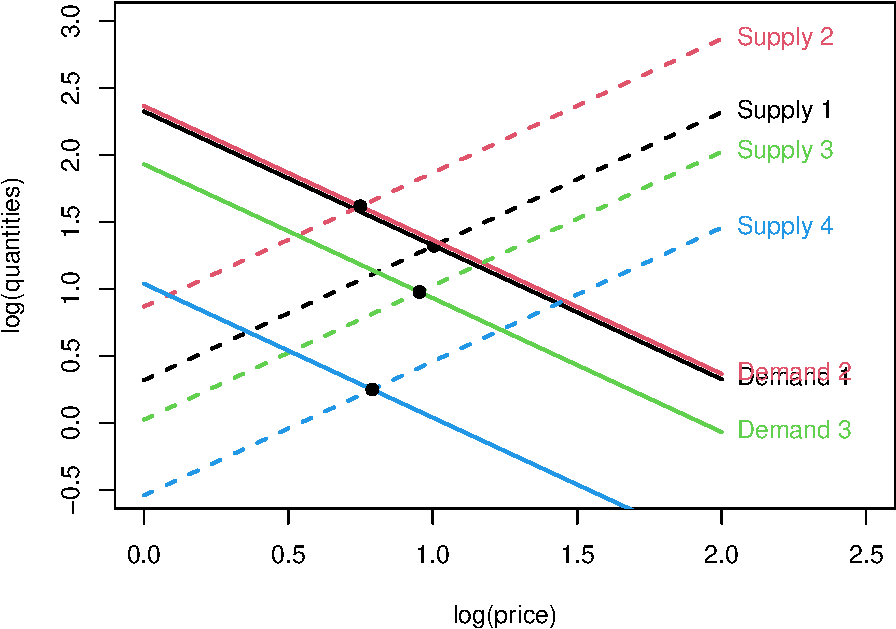
\includegraphics{EcoStat_files/figure-latex/figureIV-1.pdf}
\caption{\label{fig:figureIV}This figure illustrates the situation prevailing when estimating a price-elasticity (and the price is endogenous).}
\end{figure}

Let us use IV regressions to estimate the price elasticity of cigarette demand. For that purpose, we use the \texttt{CigarettesSW} dataset of package \texttt{AER} (these data are used by \citet{Stock_Watson_2003}). This panel dataset documents cigarette consumption for the 48 continental US States from 1985--1995. The instrument is the real tax on cigarettes arising from the state's general sales tax. The rationale is that larger general sales tax drives cigarette prices up, but the general tax is not determined by other forces affecting \(\varepsilon_t^d\).

\begin{Shaded}
\begin{Highlighting}[]
\FunctionTok{data}\NormalTok{(}\StringTok{"CigarettesSW"}\NormalTok{, }\AttributeTok{package =} \StringTok{"AER"}\NormalTok{)}
\NormalTok{CigarettesSW}\SpecialCharTok{$}\NormalTok{rprice  }\OtherTok{\textless{}{-}} \FunctionTok{with}\NormalTok{(CigarettesSW, price}\SpecialCharTok{/}\NormalTok{cpi)}
\NormalTok{CigarettesSW}\SpecialCharTok{$}\NormalTok{rincome }\OtherTok{\textless{}{-}} \FunctionTok{with}\NormalTok{(CigarettesSW, income}\SpecialCharTok{/}\NormalTok{population}\SpecialCharTok{/}\NormalTok{cpi)}
\NormalTok{CigarettesSW}\SpecialCharTok{$}\NormalTok{tdiff   }\OtherTok{\textless{}{-}} \FunctionTok{with}\NormalTok{(CigarettesSW, (taxs }\SpecialCharTok{{-}}\NormalTok{ tax)}\SpecialCharTok{/}\NormalTok{cpi)}

\DocumentationTok{\#\# model }
\NormalTok{eq.IV1 }\OtherTok{\textless{}{-}} \FunctionTok{ivreg}\NormalTok{(}\FunctionTok{log}\NormalTok{(packs) }\SpecialCharTok{\textasciitilde{}} \FunctionTok{log}\NormalTok{(rprice) }\SpecialCharTok{+} \FunctionTok{log}\NormalTok{(rincome) }\SpecialCharTok{|}
                  \FunctionTok{log}\NormalTok{(rincome) }\SpecialCharTok{+}\NormalTok{ tdiff }\SpecialCharTok{+} \FunctionTok{I}\NormalTok{(tax}\SpecialCharTok{/}\NormalTok{cpi),}
                \AttributeTok{data =}\NormalTok{ CigarettesSW, }\AttributeTok{subset =}\NormalTok{ year }\SpecialCharTok{==} \StringTok{"1995"}\NormalTok{)}
\NormalTok{eq.IV2 }\OtherTok{\textless{}{-}} \FunctionTok{ivreg}\NormalTok{(}\FunctionTok{log}\NormalTok{(packs) }\SpecialCharTok{\textasciitilde{}} \FunctionTok{log}\NormalTok{(rprice) }\SpecialCharTok{|}\NormalTok{ tdiff,}
                \AttributeTok{data =}\NormalTok{ CigarettesSW, }\AttributeTok{subset =}\NormalTok{ year }\SpecialCharTok{==} \StringTok{"1995"}\NormalTok{)}
\NormalTok{eq.no.IV }\OtherTok{\textless{}{-}} \FunctionTok{lm}\NormalTok{(}\FunctionTok{log}\NormalTok{(packs) }\SpecialCharTok{\textasciitilde{}} \FunctionTok{log}\NormalTok{(rprice) }\SpecialCharTok{+} \FunctionTok{log}\NormalTok{(rincome),}
               \AttributeTok{data =}\NormalTok{ CigarettesSW, }\AttributeTok{subset =}\NormalTok{ year }\SpecialCharTok{==} \StringTok{"1995"}\NormalTok{)}
\NormalTok{stargazer}\SpecialCharTok{::}\FunctionTok{stargazer}\NormalTok{(eq.no.IV,eq.IV1,eq.IV2,}\AttributeTok{type=}\StringTok{"text"}\NormalTok{,}\AttributeTok{no.space =} \ConstantTok{TRUE}\NormalTok{,}
                     \AttributeTok{omit.stat=}\FunctionTok{c}\NormalTok{(}\StringTok{"f"}\NormalTok{,}\StringTok{"ser"}\NormalTok{))}
\end{Highlighting}
\end{Shaded}

\begin{verbatim}
## 
## ==========================================
##                   Dependent variable:     
##              -----------------------------
##                       log(packs)          
##                 OLS       instrumental    
##                             variable      
##                 (1)       (2)       (3)   
## ------------------------------------------
## log(rprice)  -1.407*** -1.277*** -1.084***
##               (0.251)   (0.263)   (0.317) 
## log(rincome)   0.344     0.280            
##               (0.235)   (0.239)           
## Constant     10.342*** 9.895***  9.720*** 
##               (1.023)   (1.059)   (1.514) 
## ------------------------------------------
## Observations    48        48        48    
## R2             0.433     0.429     0.401  
## Adjusted R2    0.408     0.404     0.388  
## ==========================================
## Note:          *p<0.1; **p<0.05; ***p<0.01
\end{verbatim}

\begin{Shaded}
\begin{Highlighting}[]
\FunctionTok{summary}\NormalTok{(eq.IV1,}\AttributeTok{diagnostics =} \ConstantTok{TRUE}\NormalTok{)}\SpecialCharTok{$}\NormalTok{diagnostics}
\end{Highlighting}
\end{Shaded}

\begin{verbatim}
##                  df1 df2   statistic      p-value
## Weak instruments   2  44 244.7337536 1.444054e-24
## Wu-Hausman         1  44   3.0678163 8.682505e-02
## Sargan             1  NA   0.3326221 5.641191e-01
\end{verbatim}

The last three tests are interpreted as follows:

\begin{itemize}
\tightlist
\item
  Since the p-value of the first test is small, we reject the null hypothesis according to which the instrument is weak.
\item
  The small p-value of the Wu-Hausman test implies that we reject the null hypothesis according to which the OLS estimates are consistent (at the 10\% level only, though).
\item
  No over-identification (misspecification) is detected by the Sargan test (large p-value).
\end{itemize}

\end{example}

\begin{example}[Education and wage]
\protect\hypertarget{exm:IVCollegeDistance}{}\label{exm:IVCollegeDistance}

In this example, we make use of another dataset proposed by \citet{Stock_Watson_2003}, namely the \texttt{CollegeDistance} dataset.\footnote{Cross-section data from the High School and Beyond survey conducted by the Department of Education in the 80s. The survey includes students from approximately 1,100 high schools.} the objective is to estimate the effect of education on wages. Education choice is suspected to be an endogenous variable, which calls for an IV strategy. The instrumental variable is the distance to college (see, e.g., \citet{DEE20041697}).

\begin{Shaded}
\begin{Highlighting}[]
\FunctionTok{library}\NormalTok{(sem)}
\FunctionTok{data}\NormalTok{(}\StringTok{"CollegeDistance"}\NormalTok{, }\AttributeTok{package =} \StringTok{"AER"}\NormalTok{)}
\NormalTok{eq}\FloatTok{.1}\NormalTok{st.stage }\OtherTok{\textless{}{-}} \FunctionTok{lm}\NormalTok{(education }\SpecialCharTok{\textasciitilde{}}\NormalTok{ urban }\SpecialCharTok{+}\NormalTok{ gender }\SpecialCharTok{+}\NormalTok{ ethnicity }\SpecialCharTok{+}\NormalTok{ unemp }\SpecialCharTok{+}\NormalTok{ distance,}
                   \AttributeTok{data =}\NormalTok{ CollegeDistance)}
\NormalTok{CollegeDistance}\SpecialCharTok{$}\NormalTok{ed.pred}\OtherTok{\textless{}{-}} \FunctionTok{predict}\NormalTok{(eq}\FloatTok{.1}\NormalTok{st.stage)}
\NormalTok{eq}\FloatTok{.2}\NormalTok{nd.stage }\OtherTok{\textless{}{-}} \FunctionTok{lm}\NormalTok{(wage }\SpecialCharTok{\textasciitilde{}}\NormalTok{ urban }\SpecialCharTok{+}\NormalTok{ gender }\SpecialCharTok{+}\NormalTok{ ethnicity }\SpecialCharTok{+}\NormalTok{ unemp }\SpecialCharTok{+}\NormalTok{ ed.pred,}
                   \AttributeTok{data =}\NormalTok{ CollegeDistance)}
\NormalTok{eqOLS }\OtherTok{\textless{}{-}} \FunctionTok{lm}\NormalTok{(wage }\SpecialCharTok{\textasciitilde{}}\NormalTok{ urban }\SpecialCharTok{+}\NormalTok{ gender }\SpecialCharTok{+}\NormalTok{ ethnicity }\SpecialCharTok{+}\NormalTok{ unemp }\SpecialCharTok{+}\NormalTok{ education,}
            \AttributeTok{data=}\NormalTok{CollegeDistance)}
\NormalTok{eq2SLS }\OtherTok{\textless{}{-}} \FunctionTok{ivreg}\NormalTok{(wage }\SpecialCharTok{\textasciitilde{}}\NormalTok{ urban }\SpecialCharTok{+}\NormalTok{ gender }\SpecialCharTok{+}\NormalTok{ ethnicity }\SpecialCharTok{+}\NormalTok{ unemp }\SpecialCharTok{+}\NormalTok{ education}\SpecialCharTok{|}
\NormalTok{                  urban }\SpecialCharTok{+}\NormalTok{ gender }\SpecialCharTok{+}\NormalTok{ ethnicity }\SpecialCharTok{+}\NormalTok{ unemp }\SpecialCharTok{+}\NormalTok{ distance,}
                \AttributeTok{data=}\NormalTok{CollegeDistance)}
\NormalTok{stargazer}\SpecialCharTok{::}\FunctionTok{stargazer}\NormalTok{(eq}\FloatTok{.1}\NormalTok{st.stage,eq}\FloatTok{.2}\NormalTok{nd.stage,eq2SLS,eqOLS,}
                     \AttributeTok{type=}\StringTok{"text"}\NormalTok{,}\AttributeTok{no.space =} \ConstantTok{TRUE}\NormalTok{,}\AttributeTok{omit.stat =} \FunctionTok{c}\NormalTok{(}\StringTok{"f"}\NormalTok{,}\StringTok{"ser"}\NormalTok{))}
\end{Highlighting}
\end{Shaded}

\begin{verbatim}
## 
## ============================================================
##                              Dependent variable:            
##                   ------------------------------------------
##                   education               wage              
##                      OLS       OLS    instrumental    OLS   
##                                         variable            
##                      (1)       (2)        (3)         (4)   
## ------------------------------------------------------------
## urbanyes           -0.092     0.046      0.046       0.070  
##                    (0.065)   (0.045)    (0.060)     (0.045) 
## genderfemale       -0.025    -0.071*     -0.071    -0.085** 
##                    (0.052)   (0.037)    (0.050)     (0.037) 
## ethnicityafam     -0.524*** -0.227***   -0.227**   -0.556***
##                    (0.072)   (0.073)    (0.099)     (0.052) 
## ethnicityhispanic -0.275*** -0.351***  -0.351***   -0.544***
##                    (0.068)   (0.057)    (0.077)     (0.049) 
## unemp               0.010   0.139***    0.139***   0.133*** 
##                    (0.010)   (0.007)    (0.009)     (0.007) 
## distance          -0.087***                                 
##                    (0.012)                                  
## ed.pred                     0.647***                        
##                              (0.101)                        
## education                               0.647***     0.005  
##                                         (0.136)     (0.010) 
## Constant          14.061***  -0.359      -0.359    8.641*** 
##                    (0.083)   (1.412)    (1.908)     (0.157) 
## ------------------------------------------------------------
## Observations        4,739     4,739      4,739       4,739  
## R2                  0.023     0.117      -0.612      0.110  
## Adjusted R2         0.022     0.116      -0.614      0.109  
## ============================================================
## Note:                            *p<0.1; **p<0.05; ***p<0.01
\end{verbatim}

\end{example}

\hypertarget{general-regression-model-grm-and-robust-covariance-matrices}{%
\section{General Regression Model (GRM) and robust covariance matrices}\label{general-regression-model-grm-and-robust-covariance-matrices}}

The statistical inference presented above relies on strong assumptions regarding the stochastic properties of the errors. Namely, they are assumed to be mutually uncorrelated (Hypothesis \ref{hyp:noncorrelResid}) and homoskedastic (Hypothesis \ref{hyp:homoskedasticity}).

The objective of this section is to present approaches aimed at adjusting the estimate of the covariance matrix of the OLS estimator (\((\mathbf{X}'\mathbf{X})^{-1}s^2\), see Eq. \eqref{eq:sXX}), when the previous hypotheses do not hold.

\hypertarget{presentation-of-the-general-regression-model-grm}{%
\subsection{Presentation of the General Regression Model (GRM)}\label{presentation-of-the-general-regression-model-grm}}

It will prove useful to introduce the following notation:
\begin{eqnarray}
\mathbb{V}ar(\boldsymbol\varepsilon | \mathbf{X}) = \mathbb{E}(\boldsymbol\varepsilon \boldsymbol\varepsilon'| \mathbf{X}) &=& \boldsymbol\Sigma. \label{eq:assumGLS2}
\end{eqnarray}

Note that Eq. \eqref{eq:assumGLS2} is more general than Hypothesis \ref{hyp:homoskedasticity} and \ref{hyp:noncorrelResid} because the diagonal entries of \(\boldsymbol\Sigma\) may be different (as opposed to under Hypothesis \ref{hyp:homoskedasticity}), and the non-diagonal entries of \(\boldsymbol\Sigma\) can be non-null (as opposed to under Hypothesis \ref{hyp:noncorrelResid}).

\begin{definition}[General Regression Model (GRM)]
\protect\hypertarget{def:GRM}{}\label{def:GRM}Hypothesis \ref{hyp:fullrank} and \ref{hyp:exogeneity}, together with Eq. \eqref{eq:assumGLS2}, form the General Regression Model (GRM) framework.
\end{definition}

Naturally, a regression model where Hypotheses \ref{hyp:fullrank} to \ref{hyp:noncorrelResid} hold is a specific case of the GRM framework.

The GRM context notably encompasses situations of heteroskedasticity and autocorrelation:

\begin{itemize}
\item
  Heteroskedasticity:
  \begin{equation}
  \boldsymbol\Sigma = \left[  \begin{array}{cccc}
  \sigma_1^2 & 0 & \dots & 0 \\
  0 & \sigma_2^2 &  & 0 \\
  \vdots && \ddots& \vdots \\
  0 & \dots & 0 & \sigma_n^2
  \end{array} \right]. \label{eq:heteroskedasticity}
  \end{equation}
\item
  Autocorrelation:
  \begin{equation}
  \boldsymbol\Sigma = \sigma^2 \left[ \begin{array}{cccc}
  1 & \rho_{2,1} & \dots & \rho_{n,1} \\
  \rho_{2,1} & 1 &  & \vdots \\
  \vdots && \ddots& \rho_{n,n-1} \\
  \rho_{n,1} & \rho_{n,2} & \dots & 1
  \end{array} \right]. \label{eq:autocorrelation}
  \end{equation}
\end{itemize}

\begin{example}[Auto-regressive processes]
\protect\hypertarget{exm:autocorrelaaa}{}\label{exm:autocorrelaaa}Autocorrelation is common in time-series contexts (see Section \ref{TS}). In a time-series context, subscript \(i\) refers to a date.

Assume for instance that:
\begin{equation}
y_i = \mathbf{x}_i' \boldsymbol\beta + \varepsilon_i \label{eq:usual}
\end{equation}
with
\begin{equation}
\varepsilon_i = \rho \varepsilon_{i-1} + v_i, \quad v_i \sim \mathcal{N}(0,\sigma_v^2).\label{eq:usual2}
\end{equation}
In this case, we are in the GRM context, with:
\begin{equation}
\boldsymbol\Sigma =\frac{ \sigma_v^2}{1 - \rho^2} \left[    \begin{array}{cccc}
1 & \rho & \dots & \rho^{n-1} \\
\rho & 1 &  & \vdots \\
\vdots && \ddots& \rho \\
\rho^{n-1} & \rho^{n-2} & \dots & 1
\end{array} \right].\label{eq:SigmaAutocorrel}
\end{equation}
\end{example}

In some cases ---in particular when one assumes a parametric formulation for \(\boldsymbol\Sigma\)--- one can determine a better (more accurate) estimator than the OLS one. This approach is called Generalized Least Squares (GLS), which we present below.

\hypertarget{GLS}{%
\subsection{Generalized Least Squares}\label{GLS}}

Assume \(\boldsymbol\Sigma\) is known (``feasible GLS''). Because \(\boldsymbol\Sigma\) is symmetric positive, it admits a spectral decomposition of the form \(\boldsymbol\Sigma = \mathbf{C} \boldsymbol\Lambda \mathbf{C}'\), where \(\mathbf{C}\) is an orthogonal matrix (i.e.~\(\mathbf{C}\mathbf{C}'=Id\)) and \(\boldsymbol\Lambda\) is a diagonal matrix (the diagonal entries are the eigenvalues of \(\boldsymbol\Sigma\)).

We have \(\boldsymbol\Sigma = (\mathbf{P}\mathbf{P}')^{-1}\) with \(\mathbf{P} = \mathbf{C}\boldsymbol\Lambda^{-1/2}\). Consider the transformed model:
\[
\mathbf{P}'\mathbf{y} = \mathbf{P}'\mathbf{X}\boldsymbol\beta + \mathbf{P}'\boldsymbol\varepsilon \quad \mbox{or} \quad \mathbf{y}^* = \mathbf{X}^*\boldsymbol\beta + \boldsymbol\varepsilon^*.
\]
The variance of \(\boldsymbol\varepsilon^*\) is the identity matrix \(Id\). In the transformed model, OLS is BLUE (Gauss-Markow Theorem \ref{thm:GaussMarkov}).

The \textbf{Generalized least squares} estimator of \(\boldsymbol\beta\) is:
\begin{equation}
\boxed{\mathbf{b}_{GLS} = (\mathbf{X}'\boldsymbol\Sigma^{-1}\mathbf{X})^{-1}\mathbf{X}'\boldsymbol\Sigma^{-1}\mathbf{y}.}\label{eq:betaGLS}
\end{equation}
We have:
\[
\mathbb{V}ar(\mathbf{b}_{GLS}|\mathbf{X}) = (\mathbf{X}'\boldsymbol\Sigma^{-1}\mathbf{X})^{-1}.
\]

However, in general, \(\boldsymbol\Sigma\) is unknown. The GLS estimator is then said to be \emph{infeasible}. Some structure is required. Assume \(\boldsymbol\Sigma\) admits a parametric form \(\boldsymbol\Sigma(\theta)\). The estimation becomes \emph{feasible} (FGLS) if one replaces \(\boldsymbol\Sigma(\theta)\) by \(\boldsymbol\Sigma(\hat\theta)\), where \(\hat\theta\) is a consistent estimator of \(\theta\). In that case, the FGLS is asymptotically efficient (see Example \ref{exm:autocorrelaaa2}).

When \(\boldsymbol\Sigma\) has no obvious structure: the OLS (or IV) is the only estimator available. Under regularity assumptions, it remains unbiased, consistent, and asymptotically normally distributed, but not efficient. Standard inference procedures are no longer appropriate.

\begin{example}[GLS in the auto-correlation case]
\protect\hypertarget{exm:autocorrelaaa2}{}\label{exm:autocorrelaaa2}Consider the case presented in Example \ref{exm:autocorrelaaa}. Because the OLS estimate \(\mathbf{b}\) of \(\boldsymbol\beta\) is consistent, the estimates \(e_i\) of the \(\varepsilon_i\)'s also are. Consistent estimators of \(\rho\) and \(\sigma_v\) are then obtained by regressing the \(e_i\)'s on the \(e_{i-1}\)'s. Using these estimates in Eq. \eqref{eq:SigmaAutocorrel} provides a consistent estimate of \(\boldsymbol\Sigma\). Applying these steps recursively gives an efficient estimator of \(\boldsymbol\beta\) (\citet{Cochrane_Orcutt_1949}).
\end{example}

\hypertarget{asymptotic-properties-of-the-ols-estimator-in-the-grm-framework}{%
\subsection{Asymptotic properties of the OLS estimator in the GRM framework}\label{asymptotic-properties-of-the-ols-estimator-in-the-grm-framework}}

Since \(\mathbf{b} = \boldsymbol\beta + \left(\mathbf{X}'\mathbf{X}\right)^{-1} \mathbf{X}'\boldsymbol\varepsilon\) and \(\mathbb{V}ar(\boldsymbol\varepsilon|\mathbf{X})=\boldsymbol\Sigma\), we have:
\begin{equation}
\mathbb{V}ar(\mathbf{b}|\mathbf{X}) = \frac{1}{n}\left(\frac{1}{n}\mathbf{X}'\mathbf{X}\right)^{-1}\left(\frac{1}{n}\mathbf{X}'\boldsymbol\Sigma\mathbf{X}\right)\left(\frac{1}{n}\mathbf{X}'\mathbf{X}\right)^{-1}.\label{eq:xsx}
\end{equation}

Therefore, the conditional covariance matrix of the OLS estimator is not \(\sigma^2 (\mathbf{X}'\mathbf{X})^{-1}\) any longer, and using \(s^2 (\mathbf{X}'\mathbf{X})^{-1}\) for inference may be misleading. Below, we will see how to construct appropriate estimates of the covariance matrix of \(\mathbf{b}\). Before that, let us prove that the OLS estimator remains consistent in the GRM framework.

\begin{proposition}[Consistency of the OLS estimator in the GRM framework]
\protect\hypertarget{prp:XXX}{}\label{prp:XXX}If \(\mbox{plim }(\mathbf{X}'\mathbf{X}/n)\) and \(\mbox{plim }(\mathbf{X}'\boldsymbol\Sigma\mathbf{X}/n)\) are finite positive definite matrices, then \(\mbox{plim }(\mathbf{b})=\boldsymbol\beta\).
\end{proposition}

\begin{proof}
We have \(\mathbb{V}ar(\mathbf{b})=\mathbb{E}[\mathbb{V}ar(\mathbf{b}|\mathbf{X})]+\mathbb{V}ar[\mathbb{E}(\mathbf{b}|\mathbf{X})]\). Since \(\mathbb{E}(\mathbf{b}|\mathbf{X})=\boldsymbol\beta\), \(\mathbb{V}ar[\mathbb{E}(\mathbf{b}|\mathbf{X})]=0\). Eq. \eqref{eq:xsx} implies that \(\mathbb{V}ar(\mathbf{b}|\mathbf{X}) \rightarrow 0\). Hence \(\mathbf{b}\) converges in mean square, and therefore in probability (see Prop. \ref{prp:implicationsconv}).
\end{proof}

Prop. \ref{prp:AsymptGRM} gives the asymptotic distribution of the OLS estimator in the GRM framework.

\begin{proposition}[Asymptotic distribution of the OLS estimator in the GRM framework]
\protect\hypertarget{prp:AsymptGRM}{}\label{prp:AsymptGRM}If \(Q_{xx}=\mbox{plim }(\mathbf{X}'\mathbf{X}/n)\) and \(Q_{x\boldsymbol\Sigma x}=\mbox{plim }(\mathbf{X}'\boldsymbol\Sigma\mathbf{X}/n)\) are finite positive definite matrices, then:
\[
\sqrt{n}(\mathbf{b}-\boldsymbol\beta) \overset{d}{\rightarrow} \mathcal{N}(0,Q_{xx}^{-1}Q_{x\boldsymbol\Sigma x}Q_{xx}^{-1}).
\]
\end{proposition}

The IV estimator also features a normal asymptotic distribution:

\begin{proposition}[Asymptotic distribution of the IV estimator in the GRM framework]
\protect\hypertarget{prp:AsymptIVGRM}{}\label{prp:AsymptIVGRM}If regressors and IV variables are ``well-behaved'', then:
\[
\mathbf{b}_{iv} \overset{a}{\sim} \mathcal{N}(\boldsymbol\beta,\mathbf{V}_{iv}),
\]
where
\[
\mathbf{V}_{iv} = \frac{1}{n}(\mathbf{Q}^*)\mbox{ plim }\left(\frac{1}{n} \mathbf{Z}'\boldsymbol\Sigma \mathbf{Z}\right)(\mathbf{Q}^*)',
\]
with
\[
\mathbf{Q}^* = [\mathbf{Q}_{xz}\mathbf{Q}_{zz}^{-1}\mathbf{Q}_{zx}]^{-1}\mathbf{Q}_{xz}\mathbf{Q}_{zz}^{-1}.
\]
\end{proposition}

For practical purposes, one needs to have estimates of \(\boldsymbol\Sigma\) in Props. \ref{prp:AsymptGRM} or \ref{prp:AsymptIVGRM}. The complication comes from the fact that \(\boldsymbol\Sigma\) is of dimension \(n \times n\), and its estimation ---based on a sample of length \(n\)--- is therefore infeasible in the general case. Notwithstanding, looking at Eq. \eqref{eq:xsx}, it appears that one can focus on the estimation of \(Q_{x\boldsymbol\Sigma x}=\mbox{plim }(\mathbf{X}'\boldsymbol\Sigma\mathbf{X}/n)\) (or \(\mbox{plim }\left(\frac{1}{n} \mathbf{Z}'\boldsymbol\Sigma \mathbf{Z}\right)\) in the IV case). This matrix being of dimension \(K \times K\), its estimation is easier.

We have:
\begin{equation}
\frac{1}{n}\mathbf{X}'\boldsymbol\Sigma\mathbf{X} = \frac{1}{n}\sum_{i=1}^{n}\sum_{j=1}^{n}\sigma_{i,j}\mathbf{x}_i\mathbf{x}'_j. \label{eq:GeneralXSigmaX}
\end{equation}

The so-called \textbf{robust covariance matrices} are estimates of the previous matrix. Their computation is based on the fact that if \(\mathbf{b}\) is consistent, then the \(e_i\)'s are consistent estimators of the \(\varepsilon_i\)'s.

In the following sections (\ref{HAC} and \ref{Clusters}), we present two types of robust covariance matrices.

\hypertarget{HAC}{%
\subsection{HAC-robust covariance matrices}\label{HAC}}

When only heteroskedasticity prevails, i.e., when matrix \(\boldsymbol\Sigma\) is as in Eq. \eqref{eq:heteroskedasticity}, then one can use the formula proposed by \citet{White_1980} to estimate \(\frac{1}{n}\mathbf{X}'\boldsymbol\Sigma\mathbf{X}\) (see Example \ref{exm:HCheteroskedasticity}). When the residuals feature both heteroskedasticity and auto-correlation, then one can use the \citet{Newey_West_1987} approach (see Example \ref{exm:HCheterAC}).

\begin{example}[Heteroskedasticity]
\protect\hypertarget{exm:HCheteroskedasticity}{}\label{exm:HCheteroskedasticity}This is the case of Eq. \eqref{eq:heteroskedasticity}. We have \(\sigma_{i,j}=0\) for \(i \ne j\). Hence, in this case, we then need to estimate \(\frac{1}{n}\sum_{i=1}^{n}\sigma_{i}^2\mathbf{x}_i\mathbf{x}'_i\). \citet{White_1980} has shown that, under general conditions:
\begin{equation}
\mbox{plim}\left( \frac{1}{n}\sum_{i=1}^{n}\sigma_{i}^2\mathbf{x}_i\mathbf{x}'_i \right) = 
\mbox{plim}\left( \frac{1}{n}\sum_{i=1}^{n}e_{i}^2\mathbf{x}_i\mathbf{x}'_i \right). \label{eq:white}
\end{equation}
The estimator of \(\frac{1}{n}\mathbf{X}'\boldsymbol\Sigma\mathbf{X}\) therefore is:
\begin{equation}
M_{HC0} = \frac{1}{n}\mathbf{X}'
\left[
\begin{array}{cccc}
e_1^2 & 0 & \dots & 0 \\
0 & e_2^2 &  \\
\vdots & & \ddots&0 \\
0 & \dots & 0 & e_n^2
\end{array}
\right]
\mathbf{X}.\label{eq:White}
\end{equation}
where the \(e_i\) are the OLS residuals of the regression. The previous estimator is often called \textbf{HC0}. The \textbf{HC1} estimator, due to \citet{MacKinnon_White_1985}, is obtained by applying an adjustment factor \(n/(n-K)\) for the number of degrees of freedom (as in Prop. \ref{prp:expects2}). That is:
\begin{equation}
M_{HC1} = \frac{n}{n-K}M_{HC0}.\label{eq:WhiteHC1}
\end{equation}

We can illustrate the influence of heteroskedasticity using simulations. Consider the following model:
\[
y_i = x_i + \varepsilon_i, \quad \varepsilon_i \sim \mathcal{N}(0,x_i^2),
\]
where the \(x_i\)'s are i.i.d. \(t(6)\).

Here is a simulated sample (\(n=200\)) of this model:

\begin{Shaded}
\begin{Highlighting}[]
\NormalTok{n }\OtherTok{\textless{}{-}} \DecValTok{200}
\NormalTok{x }\OtherTok{\textless{}{-}} \FunctionTok{rt}\NormalTok{(n,}\AttributeTok{df=}\DecValTok{6}\NormalTok{)}
\NormalTok{y }\OtherTok{\textless{}{-}}\NormalTok{ x }\SpecialCharTok{+}\NormalTok{ x}\SpecialCharTok{*}\FunctionTok{rnorm}\NormalTok{(n)}
\FunctionTok{par}\NormalTok{(}\AttributeTok{plt=}\FunctionTok{c}\NormalTok{(.}\DecValTok{1}\NormalTok{,.}\DecValTok{95}\NormalTok{,.}\DecValTok{1}\NormalTok{,.}\DecValTok{95}\NormalTok{))}
\FunctionTok{plot}\NormalTok{(x,y,}\AttributeTok{pch=}\DecValTok{19}\NormalTok{)}
\end{Highlighting}
\end{Shaded}

\begin{figure}
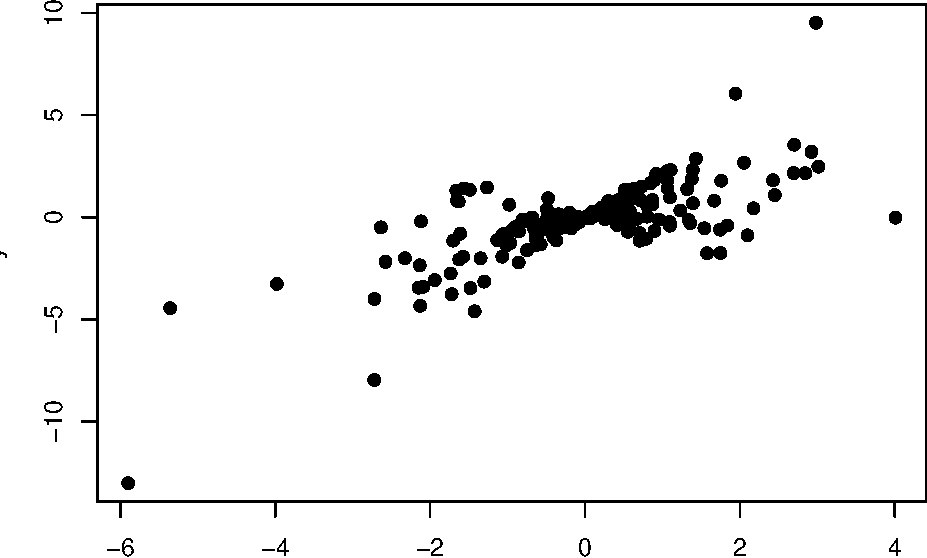
\includegraphics[width=0.9\linewidth]{EcoStat_files/figure-latex/simulHeterosk-1} \caption{Situation of heteroskedasticity. The model is $y_i = x_i + \varepsilon_i, \quad \varepsilon_i \sim \mathcal{N}(0,x_i^2)$, where the $x_i$'s are i.i.d. $t(6)$.}\label{fig:simulHeterosk}
\end{figure}

We simulate 1000 samples of the same model with \(n=200\). For each sample, we compute the OLS estimate of \(\beta\) (\(=1\)). For each of the 1000 OLS estimations, we employ (a) the standard OLS variance formula (\(s^2 (\mathbf{X}'\mathbf{X})^{-1}\)) and (b) the White formula to estimate the variance of \(b\). For each formula, we compute the average of the 1000 resulting standard deviations and compare these with the standard deviation of the 1000 OLS estimate of \(\beta\).

\begin{Shaded}
\begin{Highlighting}[]
\NormalTok{n }\OtherTok{\textless{}{-}} \DecValTok{200} \CommentTok{\# sample size}
\NormalTok{N }\OtherTok{\textless{}{-}} \DecValTok{1000} \CommentTok{\# number of simulated samples}
\NormalTok{XX }\OtherTok{\textless{}{-}} \FunctionTok{matrix}\NormalTok{(}\FunctionTok{rt}\NormalTok{(n}\SpecialCharTok{*}\NormalTok{N,}\AttributeTok{df=}\DecValTok{6}\NormalTok{),n,N)}
\NormalTok{YY }\OtherTok{\textless{}{-}} \FunctionTok{matrix}\NormalTok{(XX }\SpecialCharTok{+}\NormalTok{ XX}\SpecialCharTok{*}\FunctionTok{rnorm}\NormalTok{(n),n,N)}
\NormalTok{all\_b       }\OtherTok{\textless{}{-}} \ConstantTok{NULL}\NormalTok{;all\_V\_OLS   }\OtherTok{\textless{}{-}} \ConstantTok{NULL}\NormalTok{;all\_V\_White }\OtherTok{\textless{}{-}} \ConstantTok{NULL}
\ControlFlowTok{for}\NormalTok{(j }\ControlFlowTok{in} \DecValTok{1}\SpecialCharTok{:}\NormalTok{N)\{}
\NormalTok{  Y }\OtherTok{\textless{}{-}} \FunctionTok{matrix}\NormalTok{(YY[,j],}\AttributeTok{ncol=}\DecValTok{1}\NormalTok{)}
\NormalTok{  X }\OtherTok{\textless{}{-}} \FunctionTok{matrix}\NormalTok{(XX[,j],}\AttributeTok{ncol=}\DecValTok{1}\NormalTok{)}
\NormalTok{  b }\OtherTok{\textless{}{-}} \FunctionTok{solve}\NormalTok{(}\FunctionTok{t}\NormalTok{(X)}\SpecialCharTok{\%*\%}\NormalTok{X) }\SpecialCharTok{\%*\%} \FunctionTok{t}\NormalTok{(X)}\SpecialCharTok{\%*\%}\NormalTok{Y}
\NormalTok{  e }\OtherTok{\textless{}{-}}\NormalTok{ Y }\SpecialCharTok{{-}}\NormalTok{ X }\SpecialCharTok{\%*\%}\NormalTok{ b}
\NormalTok{  S }\OtherTok{\textless{}{-}} \DecValTok{1}\SpecialCharTok{/}\NormalTok{n }\SpecialCharTok{*} \FunctionTok{t}\NormalTok{(X) }\SpecialCharTok{\%*\%} \FunctionTok{diag}\NormalTok{(}\FunctionTok{c}\NormalTok{(e}\SpecialCharTok{\^{}}\DecValTok{2}\NormalTok{)) }\SpecialCharTok{\%*\%}\NormalTok{ X}
\NormalTok{  V\_OLS   }\OtherTok{\textless{}{-}} \FunctionTok{solve}\NormalTok{(}\FunctionTok{t}\NormalTok{(X)}\SpecialCharTok{\%*\%}\NormalTok{X) }\SpecialCharTok{*} \FunctionTok{var}\NormalTok{(e)}
\NormalTok{  V\_White }\OtherTok{\textless{}{-}} \DecValTok{1}\SpecialCharTok{/}\NormalTok{n }\SpecialCharTok{*}\NormalTok{ (}\FunctionTok{solve}\NormalTok{(}\DecValTok{1}\SpecialCharTok{/}\NormalTok{n}\SpecialCharTok{*}\FunctionTok{t}\NormalTok{(X)}\SpecialCharTok{\%*\%}\NormalTok{X)) }\SpecialCharTok{\%*\%}\NormalTok{ S }\SpecialCharTok{\%*\%}\NormalTok{ (}\FunctionTok{solve}\NormalTok{(}\DecValTok{1}\SpecialCharTok{/}\NormalTok{n}\SpecialCharTok{*}\FunctionTok{t}\NormalTok{(X)}\SpecialCharTok{\%*\%}\NormalTok{X))}
\NormalTok{  all\_b       }\OtherTok{\textless{}{-}} \FunctionTok{c}\NormalTok{(all\_b,b)}
\NormalTok{  all\_V\_OLS   }\OtherTok{\textless{}{-}} \FunctionTok{c}\NormalTok{(all\_V\_OLS,V\_OLS)}
\NormalTok{  all\_V\_White }\OtherTok{\textless{}{-}} \FunctionTok{c}\NormalTok{(all\_V\_White,V\_White)}
\NormalTok{\}}
\FunctionTok{c}\NormalTok{(}\FunctionTok{sd}\NormalTok{(all\_b),}\FunctionTok{mean}\NormalTok{(}\FunctionTok{sqrt}\NormalTok{(all\_V\_OLS)),}\FunctionTok{mean}\NormalTok{(}\FunctionTok{sqrt}\NormalTok{(all\_V\_White)))}
\end{Highlighting}
\end{Shaded}

\begin{verbatim}
## [1] 0.14024423 0.06748804 0.13973431
\end{verbatim}

The results show that the White formula yields, on average, an estimated standard deviation that is much closer to the ``true'' value than the standard OLS formula. The latter underestimate the standard deviation of \(b\).
\end{example}

In the following example, we regress GDP growth rates from the \citet{JST_2017} database on a systemic financial crisis dummy. We compute the HC0- and HC1-based standard deviations of the parameter estimate, and compare it to the one based on the standard OLS formula. The adjusted standard deviations are close to the one provided by the non-adjusted OLS formula.

\begin{Shaded}
\begin{Highlighting}[]
\FunctionTok{library}\NormalTok{(lmtest)}
\FunctionTok{library}\NormalTok{(sandwich)}
\NormalTok{nT }\OtherTok{\textless{}{-}} \FunctionTok{dim}\NormalTok{(JST)[}\DecValTok{1}\NormalTok{]}
\NormalTok{JST}\SpecialCharTok{$}\NormalTok{growth }\OtherTok{\textless{}{-}} \ConstantTok{NaN}
\NormalTok{JST}\SpecialCharTok{$}\NormalTok{growth[}\DecValTok{2}\SpecialCharTok{:}\NormalTok{nT] }\OtherTok{\textless{}{-}} \FunctionTok{log}\NormalTok{(JST}\SpecialCharTok{$}\NormalTok{rgdpbarro[}\DecValTok{2}\SpecialCharTok{:}\NormalTok{nT]}\SpecialCharTok{/}\NormalTok{JST}\SpecialCharTok{$}\NormalTok{rgdpbarro[}\DecValTok{1}\SpecialCharTok{:}\NormalTok{(nT}\DecValTok{{-}1}\NormalTok{)])}
\NormalTok{JST.red }\OtherTok{\textless{}{-}} \FunctionTok{subset}\NormalTok{(JST,year}\SpecialCharTok{\textgreater{}}\DecValTok{1950}\NormalTok{)}
\NormalTok{JST.red}\SpecialCharTok{$}\NormalTok{iso }\OtherTok{\textless{}{-}} \FunctionTok{as.factor}\NormalTok{(JST.red}\SpecialCharTok{$}\NormalTok{iso)}
\NormalTok{JST.red}\SpecialCharTok{$}\NormalTok{year }\OtherTok{\textless{}{-}} \FunctionTok{as.factor}\NormalTok{(JST.red}\SpecialCharTok{$}\NormalTok{year)}
\NormalTok{eq }\OtherTok{\textless{}{-}} \FunctionTok{lm}\NormalTok{(growth}\SpecialCharTok{\textasciitilde{}}\NormalTok{crisisJST}\SpecialCharTok{+}\NormalTok{iso,}\AttributeTok{data=}\NormalTok{JST.red)}
\FunctionTok{rbind}\NormalTok{(}\FunctionTok{coeftest}\NormalTok{(eq)[}\DecValTok{2}\NormalTok{,],}
      \FunctionTok{coeftest}\NormalTok{(eq, }\AttributeTok{vcov =} \FunctionTok{vcovHC}\NormalTok{(eq, }\AttributeTok{type =} \StringTok{"HC0"}\NormalTok{))[}\DecValTok{2}\NormalTok{,],}
      \FunctionTok{coeftest}\NormalTok{(eq, }\AttributeTok{vcov =} \FunctionTok{vcovHC}\NormalTok{(eq, }\AttributeTok{type =} \StringTok{"HC1"}\NormalTok{))[}\DecValTok{2}\NormalTok{,])}
\end{Highlighting}
\end{Shaded}

\begin{verbatim}
##         Estimate  Std. Error   t value     Pr(>|t|)
## [1,] -0.02481424 0.005490411 -4.519560 6.789284e-06
## [2,] -0.02481424 0.005605452 -4.426804 1.040602e-05
## [3,] -0.02481424 0.005648268 -4.393247 1.212105e-05
\end{verbatim}

\begin{example}[Heteroskedasticity and Autocorrelation (HAC)]
\protect\hypertarget{exm:HCheterAC}{}\label{exm:HCheterAC}\citet{Newey_West_1987} have proposed a formula to address both heteroskedasticity and auto-correlation of the residuals (Eqs. \eqref{eq:heteroskedasticity} and \eqref{eq:autocorrelation}). They show that, if the correlation between terms \(i\) and \(j\) gets sufficiently small when \(|i-j|\) increases:
\begin{eqnarray}
&&\mbox{plim} \left( \frac{1}{n}\sum_{i=1}^{n}\sum_{j=1}^{n}\sigma_{i,j}\mathbf{x}_i\mathbf{x}'_j \right) \approx  \\
&&\mbox{plim} \left( \frac{1}{n}\sum_{t=1}^{n}e_{t}^2\mathbf{x}_t\mathbf{x}'_t +
\frac{1}{n}\sum_{\ell=1}^{L}\sum_{t=\ell+1}^{n}w_\ell e_{t}e_{t-\ell}(\mathbf{x}_t\mathbf{x}'_{t-\ell} + \mathbf{x}_{t-\ell}\mathbf{x}'_{t})
\right), \nonumber \label{eq:NW}
\end{eqnarray}
where \(w_\ell = 1 - \ell/(L+1)\) (with \(L\) large).

Let us illustrate the influence of autocorrelation using simulations. We consider the following model:
\begin{equation}
y_i = x_i + \varepsilon_i, \quad \varepsilon_i \sim \mathcal{N}(0,x_i^2),\label{eq:simul11}
\end{equation}
where the \(x_i\)'s and the \(\varepsilon_i\)'s are such that:
\begin{equation}
x_i = 0.8 x_{i-1} + u_i \quad and \quad \varepsilon_i = 0.8 \varepsilon_{i-1} + v_i, \label{eq:simul22}
\end{equation}
where the \(u_i\)'s and the \(v_i\)'s are i.i.d. \(\mathcal{N}(0,1)\).

We simulate 500 samples of the same model with \(n=200\). For each sample, we compute the OLS estimate of \(\beta\) (=1). For each of the 1000 OLS estimations, we employ (a) the standard OLS variance formula (\(s^2 (\mathbf{X}'\mathbf{X})^{-1}\)), (b) the White formula, and (c) the Newey-West formula to estimate the variance of \(b\). For each formula, we compute the average of the 500 resulting standard deviations and compare these with the standard deviation of the 500 OLS estimate of \(\beta\).

\begin{Shaded}
\begin{Highlighting}[]
\FunctionTok{library}\NormalTok{(AEC)}
\NormalTok{n }\OtherTok{\textless{}{-}} \DecValTok{100} \CommentTok{\# sample length}
\NormalTok{nb.sim }\OtherTok{\textless{}{-}} \DecValTok{500} \CommentTok{\# number of simulated samples}
\NormalTok{all.b }\OtherTok{\textless{}{-}} \ConstantTok{NULL}\NormalTok{;all.OLS.stdv.b }\OtherTok{\textless{}{-}} \ConstantTok{NULL}
\NormalTok{all.Whi.stdv.b }\OtherTok{\textless{}{-}} \ConstantTok{NULL}\NormalTok{;all.NW.stdv.b }\OtherTok{\textless{}{-}} \ConstantTok{NULL}
\ControlFlowTok{for}\NormalTok{(i }\ControlFlowTok{in} \DecValTok{1}\SpecialCharTok{:}\NormalTok{nb.sim)\{}
\NormalTok{  eps }\OtherTok{\textless{}{-}} \FunctionTok{rnorm}\NormalTok{(n);x }\OtherTok{\textless{}{-}} \FunctionTok{rnorm}\NormalTok{(n)}
  \ControlFlowTok{for}\NormalTok{(i }\ControlFlowTok{in} \DecValTok{2}\SpecialCharTok{:}\NormalTok{n)\{}
\NormalTok{    eps[i] }\OtherTok{\textless{}{-}}\NormalTok{ eps[i] }\SpecialCharTok{+}\NormalTok{ .}\DecValTok{8}\SpecialCharTok{*}\NormalTok{eps[i}\DecValTok{{-}1}\NormalTok{]}
\NormalTok{    x[i]   }\OtherTok{\textless{}{-}}\NormalTok{ x[i]   }\SpecialCharTok{+}\NormalTok{ .}\DecValTok{8}\SpecialCharTok{*}\NormalTok{x[i}\DecValTok{{-}1}\NormalTok{]}
\NormalTok{  \}}
\NormalTok{  y }\OtherTok{\textless{}{-}}\NormalTok{ x }\SpecialCharTok{+}\NormalTok{ eps}
\NormalTok{  eq }\OtherTok{\textless{}{-}} \FunctionTok{lm}\NormalTok{(y}\SpecialCharTok{\textasciitilde{}}\NormalTok{x)}
\NormalTok{  all.b }\OtherTok{\textless{}{-}} \FunctionTok{c}\NormalTok{(all.b,eq}\SpecialCharTok{$}\NormalTok{coefficients[}\DecValTok{2}\NormalTok{])}
\NormalTok{  all.OLS.stdv.b }\OtherTok{\textless{}{-}} \FunctionTok{c}\NormalTok{(all.OLS.stdv.b,}\FunctionTok{summary}\NormalTok{(eq)}\SpecialCharTok{$}\NormalTok{coefficients[}\DecValTok{2}\NormalTok{,}\DecValTok{2}\NormalTok{])}
\NormalTok{  X }\OtherTok{\textless{}{-}} \FunctionTok{cbind}\NormalTok{(}\FunctionTok{rep}\NormalTok{(}\DecValTok{1}\NormalTok{,n),x)}
\NormalTok{  XX }\OtherTok{\textless{}{-}} \FunctionTok{t}\NormalTok{(X) }\SpecialCharTok{\%*\%}\NormalTok{ X;XX\_1 }\OtherTok{\textless{}{-}} \FunctionTok{solve}\NormalTok{(XX)}
\NormalTok{  E2 }\OtherTok{\textless{}{-}} \FunctionTok{diag}\NormalTok{(eq}\SpecialCharTok{$}\NormalTok{residuals}\SpecialCharTok{\^{}}\DecValTok{2}\NormalTok{)}
\NormalTok{  White.V }\OtherTok{\textless{}{-}}\NormalTok{ XX\_1 }\SpecialCharTok{\%*\%}\NormalTok{ (}\FunctionTok{t}\NormalTok{(X) }\SpecialCharTok{\%*\%}\NormalTok{ E2 }\SpecialCharTok{\%*\%}\NormalTok{ X) }\SpecialCharTok{\%*\%}\NormalTok{ XX\_1}
\NormalTok{  all.Whi.stdv.b }\OtherTok{\textless{}{-}} \FunctionTok{c}\NormalTok{(all.Whi.stdv.b,}\FunctionTok{sqrt}\NormalTok{(White.V[}\DecValTok{2}\NormalTok{,}\DecValTok{2}\NormalTok{]))}
  \CommentTok{\# HAC:}
\NormalTok{  U }\OtherTok{\textless{}{-}}\NormalTok{ X }\SpecialCharTok{*} \FunctionTok{cbind}\NormalTok{(eq}\SpecialCharTok{$}\NormalTok{residuals,eq}\SpecialCharTok{$}\NormalTok{residuals)}
\NormalTok{  XSigmaX }\OtherTok{\textless{}{-}} \FunctionTok{NW.LongRunVariance}\NormalTok{(U,}\DecValTok{5}\NormalTok{)}
\NormalTok{  NW.V }\OtherTok{\textless{}{-}} \DecValTok{1}\SpecialCharTok{/}\NormalTok{n }\SpecialCharTok{*}\NormalTok{ (n}\SpecialCharTok{*}\NormalTok{XX\_1) }\SpecialCharTok{\%*\%}\NormalTok{ XSigmaX }\SpecialCharTok{\%*\%}\NormalTok{ (n}\SpecialCharTok{*}\NormalTok{XX\_1)}
\NormalTok{  all.NW.stdv.b }\OtherTok{\textless{}{-}} \FunctionTok{c}\NormalTok{(all.NW.stdv.b,}\FunctionTok{sqrt}\NormalTok{(NW.V[}\DecValTok{2}\NormalTok{,}\DecValTok{2}\NormalTok{]))}
\NormalTok{\}}
\FunctionTok{cbind}\NormalTok{(}\FunctionTok{sd}\NormalTok{(all.b),}\FunctionTok{mean}\NormalTok{(all.OLS.stdv.b),}
      \FunctionTok{mean}\NormalTok{(all.Whi.stdv.b),}\FunctionTok{mean}\NormalTok{(all.NW.stdv.b))}
\end{Highlighting}
\end{Shaded}

\begin{verbatim}
##          [,1]      [,2]      [,3]     [,4]
## [1,] 0.201172 0.1013048 0.0962689 0.146974
\end{verbatim}

The results show that the Newey-West formula yields, on average, an estimated standard deviation that is closer to the ``true'' value than the standard OLS formula. The latter underestimate the standard deviation of \(b\).
\end{example}

What precedes suggest that, when the residuals feature autocorrelation, it is important to use appropriately adjusted covariance matrices to make statistical inference. How to detect autocorrelation in residuals? A popular test has been proposed by \citet{Durbin_Watson_1950} and \citet{Durbin_Watson_1951}. The Durbin-Watson test statistic is:
\[
DW = \frac{\sum_{i=2}^{n}(e_i - e_{i-1})^2}{\sum_{i=1}^{n}e_i^2}= 2(1 - r) - \underbrace{\frac{e_1^2 + e_n^2}{\sum_{i=1}^{n}e_i^2}}_{\overset{p}{\rightarrow} 0},
\]
where \(r\) is the slope in the regression of the \(e_i\)'s on the \(e_{i-1}\)'s, i.e.:
\[
r = \frac{\sum_{i=2}^{n}e_i e_{i-1}}{\sum_{i=1}^{n-1}e_i^2}.
\]
(\(r\) is a consistent estimator of \(\mathbb{C}or(\varepsilon_i,\varepsilon_{i-1})\), i.e.~\(\rho\) in Eq. \eqref{eq:usual2}.)

The one-sided test for \(H_0\): \(\rho=0\) against \(H_1\): \(\rho>0\) is carried out by comparing \(DW\) to values \(d_L(T, K)\) and \(d_U(T, K)\):
\[
\left\{
\begin{array}{ll}
\mbox{If $DW < d_L$,}&\mbox{ the null hypothesis is rejected;}\\
\mbox{if $DW > d_U$,}&\mbox{ the hypothesis is not rejected;}\\
\mbox{If $d_L \le DW \le d_U$,} &\mbox{ no conclusion is drawn.}
\end{array}
\right.
\]

\begin{example}[Durbin-Watson test]
\protect\hypertarget{exm:DurbinWats}{}\label{exm:DurbinWats}

We regress the short-term nominal US interest rate on inflation. We then employ the Durbin-Watson test to see whether the residuals are auto-correlated (which is quite obviously the case).

\begin{Shaded}
\begin{Highlighting}[]
\FunctionTok{library}\NormalTok{(car)}
\NormalTok{data }\OtherTok{\textless{}{-}} \FunctionTok{subset}\NormalTok{(JST,iso}\SpecialCharTok{==}\StringTok{"USA"}\NormalTok{);T }\OtherTok{\textless{}{-}} \FunctionTok{dim}\NormalTok{(data)[}\DecValTok{1}\NormalTok{]}
\NormalTok{data}\SpecialCharTok{$}\NormalTok{infl }\OtherTok{\textless{}{-}} \FunctionTok{c}\NormalTok{(}\ConstantTok{NaN}\NormalTok{,}\DecValTok{100}\SpecialCharTok{*}\FunctionTok{log}\NormalTok{(data}\SpecialCharTok{$}\NormalTok{cpi[}\DecValTok{2}\SpecialCharTok{:}\NormalTok{T]}\SpecialCharTok{/}\NormalTok{data}\SpecialCharTok{$}\NormalTok{cpi[}\DecValTok{1}\SpecialCharTok{:}\NormalTok{(T}\DecValTok{{-}1}\NormalTok{)]))}
\NormalTok{data}\SpecialCharTok{$}\NormalTok{infl[(data}\SpecialCharTok{$}\NormalTok{infl}\SpecialCharTok{\textless{}} \SpecialCharTok{{-}}\DecValTok{5}\NormalTok{)}\SpecialCharTok{|}\NormalTok{(data}\SpecialCharTok{$}\NormalTok{infl}\SpecialCharTok{\textgreater{}}\DecValTok{10}\NormalTok{)] }\OtherTok{\textless{}{-}} \ConstantTok{NaN}
\FunctionTok{par}\NormalTok{(}\AttributeTok{mfrow=}\FunctionTok{c}\NormalTok{(}\DecValTok{1}\NormalTok{,}\DecValTok{2}\NormalTok{))}
\FunctionTok{plot}\NormalTok{(data}\SpecialCharTok{$}\NormalTok{year,data}\SpecialCharTok{$}\NormalTok{stir,}\AttributeTok{ylim=}\FunctionTok{c}\NormalTok{(}\SpecialCharTok{{-}}\DecValTok{10}\NormalTok{,}\DecValTok{20}\NormalTok{),}\AttributeTok{type=}\StringTok{"l"}\NormalTok{,}\AttributeTok{lwd=}\DecValTok{2}\NormalTok{,}\AttributeTok{xlab=}\StringTok{""}\NormalTok{,}
     \AttributeTok{ylab=}\StringTok{""}\NormalTok{,}\AttributeTok{main=}\StringTok{"Nominal rate and inflation"}\NormalTok{)}
\FunctionTok{lines}\NormalTok{(data}\SpecialCharTok{$}\NormalTok{year,data}\SpecialCharTok{$}\NormalTok{infl,}\AttributeTok{col=}\StringTok{"red"}\NormalTok{,}\AttributeTok{lwd=}\DecValTok{2}\NormalTok{)}
\NormalTok{eq }\OtherTok{\textless{}{-}} \FunctionTok{lm}\NormalTok{(stir}\SpecialCharTok{\textasciitilde{}}\NormalTok{infl,}\AttributeTok{data=}\NormalTok{data)}
\FunctionTok{plot}\NormalTok{(eq}\SpecialCharTok{$}\NormalTok{residuals,}\AttributeTok{type=}\StringTok{"l"}\NormalTok{,}\AttributeTok{col=}\StringTok{"blue"}\NormalTok{,}\AttributeTok{main=}\StringTok{"Residuals"}\NormalTok{,}\AttributeTok{xlab=}\StringTok{""}\NormalTok{,}\AttributeTok{ylab=}\StringTok{""}\NormalTok{)}
\end{Highlighting}
\end{Shaded}

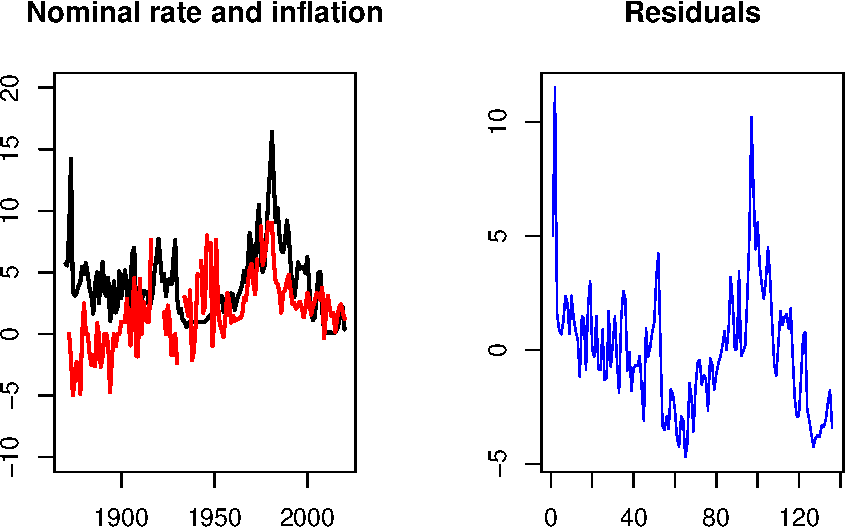
\includegraphics{EcoStat_files/figure-latex/DB-1.pdf}

\begin{Shaded}
\begin{Highlighting}[]
\FunctionTok{durbinWatsonTest}\NormalTok{(eq)}
\end{Highlighting}
\end{Shaded}

\begin{verbatim}
##  lag Autocorrelation D-W Statistic p-value
##    1       0.7321902     0.4984178       0
##  Alternative hypothesis: rho != 0
\end{verbatim}

\end{example}

\hypertarget{Clusters}{%
\subsection{Cluster-robust covariance matrices}\label{Clusters}}

The present section is based on \citet{MACKINNON2022}; another useful reference is \citet{Cameron_Miller_2014}. We will see how one can approximate \(Q_{x\boldsymbol\Sigma x}=\mbox{plim }(\mathbf{X}'\boldsymbol\Sigma\mathbf{X}/n)\) (see Prop. \ref{prp:AsymptGRM}) when the dataset can be decomposed into \emph{clusters}. These clusters constitute a partition of the sample, and they are such that the error terms may be correlated within a given cluster, but not across different clusters. A cluster may, e.g., gathers entities from a given geographical area, from the same industry, or same age cohort.

The OLS estimator satisfies:
\begin{equation}
\mathbf{b} = \boldsymbol\beta + (\mathbf{X}'\mathbf{X})^{-1}\mathbf{X}'\boldsymbol\varepsilon.\label{eq:BBB}
\end{equation}
Consider a set \(\{n_1,n_2,\dots,n_G\}\) s.t. \(n=\sum_g n_g\), on which is based the following decomposition of \(\mathbf{X}\):
\[
\mathbf{X} = \left[
\begin{array}{c}
\mathbf{X}_1 \\
\mathbf{X}_1 \\
\vdots\\
\mathbf{X}_G
\end{array}
\right].
\]
With these notations, Eq. \eqref{eq:BBB} rewrites:
\begin{equation}
\mathbf{b} - \boldsymbol\beta = \left(\sum_{g=1}^G \mathbf{X}_g'\mathbf{X}_g\right)^{-1}\sum_{g=1}^G \mathbf{s}_g,\label{eq:cluster1}
\end{equation}
where
\begin{equation}
\mathbf{s}_g = \mathbf{X}_g'\boldsymbol\varepsilon_g \label{eq:definiS}
\end{equation}
denotes the score vector (of dimension \(K \times 1\)) associated with the \(g^{th}\) cluster.

If the model is correctly specified then \(\mathbb{E}(\mathbf{s}_g)=0\) for all clusters \(g\). Note that Eq. \eqref{eq:cluster1} is valid for any partition of \(\{1,\dots,n\}\). Dividing the sample into clusters becomes meaningful if we further assume that the following hypothesis holds:

\begin{hypothesis}[Clusters]
\protect\hypertarget{hyp:cluster}{}\label{hyp:cluster}We have:
\[
(i)\; \mathbb{E}(\mathbf{s}_g\mathbf{s}_g')=\Sigma_g,\quad (ii)\; \mathbb{E}(\mathbf{s}_g\mathbf{s}_q')=0,\;g \ne q,
\]
where \(s_g\) is defined in Eq. \eqref{eq:definiS}.
\end{hypothesis}

The real assumption here is \((ii)\); the first one simply gives a notation for the covariance matrix of the score associated with the \(g^{th}\) cluster. Remark that these covariance matrices can differ across clusters. That is, \emph{cluster-based inference is robust against both heteroskedasticity and intra-cluster dependence without imposing any restrictions on the (unknown) form of either of them}.

Naturally, matrix \(\Sigma_g\) depends on the covariance structure of the \(\varepsilon\)'s. In particular, if \(\Omega_g = \mathbb{E}(\boldsymbol\varepsilon_g\boldsymbol\varepsilon_g'|\mathbf{X}_g)\), then we have \(\Sigma_g = \mathbb{E}(\mathbf{X}_g'\Omega_g\mathbf{X}_g)\).

Under Hypothesis \ref{hyp:cluster}, it comes that the conditional covariance matrix of \(\mathbf{b}\) is:
\begin{equation}
\left(\mathbf{X}'\mathbf{X}\right)^{-1}\left(\sum_{g=1}^G \Sigma_g\right)\left(\mathbf{X}'\mathbf{X}\right)^{-1}\label{eq:cluster2}
\end{equation}

Let us denote by \(\varepsilon_{g,i}\) the error associated with the \(i^{th}\) component of vector \(\boldsymbol\varepsilon_g\). Consider the special case where \(\mathbb{E}(\varepsilon_{g,i} \varepsilon_{g,j}|\mathbf{X}_g)=\sigma^2\mathbb{I}_{\{i=j\}}\), then Eq. \eqref{eq:cluster2} gives the standard expression \(\sigma^2\left(\mathbf{X}'\mathbf{X}\right)^{-1}\) (see Eq. \eqref{eq:distriBcondi}).

If we have \(\mathbb{E}(\varepsilon_{gi} \varepsilon_{gj}|\mathbf{X}_g)=\sigma_{gi}^2\mathbb{I}_{\{i=j\}}\), then we fall in the case addressed by the White formula (see Example \ref{exm:HCheteroskedasticity}). That is, in this case, the conditional covariance matrix of \(\mathbf{b}\) is:
\[
\left(\mathbf{X}'\mathbf{X}\right)^{-1}\left(\mathbf{X}'\left[  \begin{array}{cccc}
\sigma_1^2 & 0 & \dots & 0 \\
0 & \sigma_2^2 &  & 0 \\
\vdots && \ddots& \vdots \\
0 & \dots & 0 & \sigma_n^2
\end{array} \right]\mathbf{X}\right)\left(\mathbf{X}'\mathbf{X}\right)^{-1}.
\]
As in \citet{White_1980}, the natural way to approach the conditional covariance given in Eq. \eqref{eq:cluster2} consists in replacing the \(\Sigma_g\) matrices by their sample equivalent, i.e.~\(\widehat{\Sigma}_g=\mathbf{X}_g'\mathbf{e}_g\mathbf{e}_g'\mathbf{X}_g\). Adding corrections for the number of degrees of freedom, this leads to the following estimate of the covariance matrix of \(\mathbf{b}\):
\begin{equation}
\frac{G(n-1)}{(G-1)(n-K)}\left(\mathbf{X}'\mathbf{X}\right)^{-1}\left(\sum_{g=1}^G\widehat{\Sigma}_g\right) \left(\mathbf{X}'\mathbf{X}\right)^{-1}. \label{eq:AsymptCL}
\end{equation}
The previous estimate is CRCV1 in \citet{MACKINNON2022}. Note that we indeed find the White-MacKinnon estimator (Eq. \eqref{eq:WhiteHC1}) when \(G=n\).

Remark that if there was only one cluster (\(G=1\)), and neglecting the degree-of-freedom correction, we would have:
\[
\left(\mathbf{X}'\mathbf{X}\right)^{-1}\left(\mathbf{X}'\mathbf{e}\mathbf{e}'\mathbf{X}\right) \left(\mathbf{X}'\mathbf{X}\right)^{-1} = 0
\]
because \(\mathbf{X}'\mathbf{e}=0\). Hence, having large clusters does not necessarily increase variance.

Often, when working with panel data (see Chapter \ref{Panel}), we want to cluster in different dimensions. A typical case is when the data are indexed by both individuals (\(i\)) and time (\(t\)). In that case, we may indeed suspect that: (a) the residuals are correlated across clusters of dates (e.g., with monthly data, a cluster may be one year) and (b) the residuals are correlated across clusters of individuals (e.g., with data at the county level a cluster may be a state). In this case, one can employ \textbf{two-way clustering}.

Formally, consider two distinct partitions of the data: one through index \(g\), with \(g \in \{1,\dots,G\}\), and the other through index \(h\), with \(h \in \{1,\dots,H\}\). Accordingly, we denote by \(\mathbf{X}_{g,h}\) the submatrix of \(\mathbf{X}\) that contains the explanatory variables corresponding to clusters \(g\) and \(h\) (e.g., the firms of a given country \(g\) at a given date \(h\)). We also denote by \(\mathbf{X}_{g,\bullet}\) (respectively \(\mathbf{X}_{\bullet,h}\)) the submatrix of \(\mathbf{X}\) containing all explanatory variables pertaining to cluster \(g\), for all possible values of \(h\) (resp. to cluster \(h\), for all possible values of \(g\)).

We will make the following assumption:

\begin{hypothesis}[Two-way clusters]
\protect\hypertarget{hyp:twowaycluster}{}\label{hyp:twowaycluster}We have:
\begin{eqnarray*}
&&\mathbb{E}(\mathbf{s}_{g,\bullet}\mathbf{s}_{g,\bullet}')=\Sigma_g,\quad \mathbb{E}(\mathbf{s}_{\bullet,h}\mathbf{s}_{\bullet,h}')=\Sigma^*_h,\quad \mathbb{E}(\mathbf{s}_{g,h}\mathbf{s}_{g,h}')=\Sigma_{g,h},\\ &&\mathbb{E}(\mathbf{s}_{g,h}\mathbf{s}_{q,k}')=0\;\mbox{if }g\neq q\mbox{ and }h \ne k.
\end{eqnarray*}
\end{hypothesis}

\begin{proposition}[Covariance of scores in the two-way-cluster setup]
\protect\hypertarget{prp:twoWayCov}{}\label{prp:twoWayCov}Under this assumption, the matrix of covariance of the scores is given by:
\[
\Sigma = \sum_{g=1}^G \Sigma_{g} + \sum_{h=1}^H \Sigma^*_{h} - \sum_{g=1}^G\sum_{h=1}^H \Sigma_{g,h}.
\]
(The last term on the right-hand side must be subtracted in order to avoid double counting.)
\end{proposition}

\begin{proof}
We have:
\begin{eqnarray*}
\Sigma &=& \sum_{g=1}^G\sum_{q=1}^G\sum_{h=1}^H\sum_{k=1}^H \mathbf{s}_{g,h}\mathbf{s}_{q,k}'\\
&=& \sum_{g=1}^G\underbrace{\left(\sum_{h=1}^H\sum_{k=1}^H \mathbf{s}_{g,h}\mathbf{s}_{g,k}'\right)}_{=\Sigma_g}+\sum_{h=1}^H\underbrace{\left(\sum_{g=1}^G\sum_{q=1}^G \mathbf{s}_{g,h}\mathbf{s}_{q,h}'\right)}_{=\Sigma^*_h}-\sum_{g=1}^G\sum_{h=1}^H \mathbf{s}_{g,h}\mathbf{s}_{g,h}',
\end{eqnarray*}
which gives the result.
\end{proof}

The asymptotic theory can be based on two different approaches: (i) large number of clusters (common case), and (ii) fixed number of clusters but large number of observations in each cluster (see Subsections 4.1 and 4.2 in \citet{MACKINNON2022}). The more variable the \(N_g\)'s (clusters' sizes are heterogeneous in terms of size), the less reliable asymptotic inference based on Eq. \eqref{eq:AsymptCL}, especially when a very few clusters are unusually large, or when the distribution of the data is heavy-tailed. These issues are somehow mitigated when the clusters have an approximate factor structure.

In practice, \(\Sigma\) is estimated by:
\[
\widehat{\Sigma} = \sum_{g=1}^G \widehat{\mathbf{s}}_{g,\bullet}\widehat{\mathbf{s}}_{g,\bullet}' + \sum_{h=1}^H \widehat{\mathbf{s}}_{\bullet,h}\widehat{\mathbf{s}}_{\bullet,h} - \sum_{g=1}^G\sum_{h=1}^H \widehat{\mathbf{s}}_{g,h}\widehat{\mathbf{s}}_{g,h}',
\]
and we use:
\[
\widehat{\mathbb{V}ar}(\mathbf{b}) = \left(\mathbf{X}'\mathbf{X}\right)^{-1}\widehat{\Sigma}\left(\mathbf{X}'\mathbf{X}\right)^{-1}.
\]

As an alternative to the asymptotic approximation to the distribution of a statistic of interest, one can resort to bootstrap approximation (see Section 5 of \citet{MACKINNON2022}). In R, the package \texttt{fwildclusterboot} allows to implement such approaches.\footnote{See, e.g., \href{https://cran.r-project.org/web/packages/fwildclusterboot/vignettes/fwildclusterboot.html}{this tutorial by Alexander Fischer}.}

Let us come back to the analysis of the effect of systemic financial crises on GDP growth. Clustering the data at the country level and, further, at both the country and time levels gives the following:

\begin{Shaded}
\begin{Highlighting}[]
\NormalTok{eq }\OtherTok{\textless{}{-}} \FunctionTok{lm}\NormalTok{(growth}\SpecialCharTok{\textasciitilde{}}\NormalTok{crisisJST}\SpecialCharTok{+}\NormalTok{iso,}\AttributeTok{data=}\NormalTok{JST.red)}
\FunctionTok{rbind}\NormalTok{(}\FunctionTok{coeftest}\NormalTok{(eq)[}\DecValTok{2}\NormalTok{,],}
      \FunctionTok{coeftest}\NormalTok{(eq, }\AttributeTok{vcov =} \FunctionTok{vcovHC}\NormalTok{(eq, }\AttributeTok{type =} \StringTok{"HC1"}\NormalTok{))[}\DecValTok{2}\NormalTok{,],}
      \FunctionTok{coeftest}\NormalTok{(eq, }\AttributeTok{vcov =} \FunctionTok{vcovCL}\NormalTok{(eq, }\AttributeTok{cluster =}\NormalTok{ JST.red[, }\FunctionTok{c}\NormalTok{(}\StringTok{"iso"}\NormalTok{)]))[}\DecValTok{2}\NormalTok{,],}
      \FunctionTok{coeftest}\NormalTok{(eq, }\AttributeTok{vcov =} \FunctionTok{vcovCL}\NormalTok{(eq, }\AttributeTok{cluster =}\NormalTok{ JST.red[, }\FunctionTok{c}\NormalTok{(}\StringTok{"iso"}\NormalTok{,}\StringTok{"year"}\NormalTok{)]))[}\DecValTok{2}\NormalTok{,])}
\end{Highlighting}
\end{Shaded}

\begin{verbatim}
##         Estimate  Std. Error   t value     Pr(>|t|)
## [1,] -0.02481424 0.005490411 -4.519560 6.789284e-06
## [2,] -0.02481424 0.005648268 -4.393247 1.212105e-05
## [3,] -0.02481424 0.005847708 -4.243413 2.365508e-05
## [4,] -0.02481424 0.006546931 -3.790209 1.577572e-04
\end{verbatim}

\hypertarget{shrinkage-methods}{%
\section{Shrinkage methods}\label{shrinkage-methods}}

Chosing the appropriate explanatory variables is often complicated, especially in the presence of many potentially relevant covariates. Keeping a large number of covariates results in large standard deviations for the estimated parameters (see Section \ref{irrelevant}). In order to address this issue, shrinkage methods have been designed. The objective of these methods is to help select a limited number of variables by shrinking the regression coefficients of the less useful variables towards zero. The two best-known shrinkage techniques are \textbf{ridge regression} and the \textbf{lasso} approach.\footnote{See \citet{Tibshirani_2011} for a review of the lasso approach. See also Section 6.2 of \citet{James2013}.} In both cases (ridge and lasso), the OLS minimization problem (see Section \ref{LSquares}), i.e.,
\begin{equation}
\mathbf{b} = \underset{\boldsymbol\beta}{\mbox{argmin}}\; \sum_{i=1}^n(y_i - \mathbf{x}_i'\boldsymbol\beta)^2
\end{equation}
is replaced with the following:
\begin{equation}
\mathbf{b}_\lambda = \underset{\boldsymbol\beta}{\mbox{argmin}}\; \sum_{i=1}^n(y_i - \mathbf{x}_i'\boldsymbol\beta)^2 + \lambda f(\boldsymbol\beta),\label{eq:minLasso}
\end{equation}
where \(\lambda f(\boldsymbol\beta)\) is a penalty term that positively depends on the ``size'' of the components of \(\boldsymbol\beta\). This term is called the \emph{shrinkage penalty} term.

Specifically, assuming that the vector \(\mathbf{x}_i\) of potential covariates is of dimension \(K \times 1\), we have:
\begin{eqnarray*}
f(\boldsymbol\beta) & = & \sum_{j=1}^K \beta_j^2 \quad \mbox{in the ridge case ($\ell_2$ norm)},\\
f(\boldsymbol\beta) & = & \sum_{j=1}^K |\beta_j| \quad \mbox{in the lasso case ($\ell_1$ norm)}.
\end{eqnarray*}

In most cases, we do not want to involve the intercept in the set of parameters to shrink, and the preceding equations are respectively replaced with:
\begin{eqnarray*}
f(\boldsymbol\beta) & = & \sum_{j=2}^K \beta_j^2 \quad \mbox{(ridge)},\\
f(\boldsymbol\beta) & = & \sum_{j=2}^K |\beta_j| \quad \mbox{(lasso)}.
\end{eqnarray*}

The nature of the penalty ---based on either the \(\ell_1\) or the \(\ell_2\) norm--- implies a different behaviour of the parameter estimates when \(\lambda\) ---the \emph{tuning parameter}--- grows. In the ridge regression, coefficient estimates go to zero (shrinkage); in the lasso case, some coefficients reach zero when \(\lambda\) reach some values. In other words, while ridge regression achieve shrinkage, lasso regressions achieve shrinkage \emph{and} variable selection.

Parameter \(\lambda\) has to be determined separately from the minimization problem of Eq. \eqref{eq:minLasso}. One can combine standard criteria (e.g., BIC or Akaike) for this purpose.

In R, one can use the \texttt{glmnet} package to run ridge and lasso regressions. In the following example, we employ this package to model interest rates proposed to debtors, using data extracted from the \href{https://www.kaggle.com/datasets/ethon0426/lending-club-20072020q1}{Lending Club} platform.

To begin with, let us define the variables we want to consider:

\begin{Shaded}
\begin{Highlighting}[]
\FunctionTok{library}\NormalTok{(AEC)}
\FunctionTok{library}\NormalTok{(glmnet)}
\NormalTok{credit}\SpecialCharTok{$}\NormalTok{owner }\OtherTok{\textless{}{-}} \DecValTok{1}\SpecialCharTok{*}\NormalTok{(credit}\SpecialCharTok{$}\NormalTok{home\_ownership}\SpecialCharTok{==}\StringTok{"OWN"}\NormalTok{)}
\NormalTok{credit}\SpecialCharTok{$}\NormalTok{renter }\OtherTok{\textless{}{-}} \DecValTok{1}\SpecialCharTok{*}\NormalTok{(credit}\SpecialCharTok{$}\NormalTok{home\_ownership}\SpecialCharTok{==}\StringTok{"MORTGAGE"}\NormalTok{)}
\NormalTok{credit}\SpecialCharTok{$}\NormalTok{verification\_status }\OtherTok{\textless{}{-}} \DecValTok{1}\SpecialCharTok{*}\NormalTok{(credit}\SpecialCharTok{$}\NormalTok{verification\_status}\SpecialCharTok{==}\StringTok{"Not Verified"}\NormalTok{)}
\NormalTok{credit}\SpecialCharTok{$}\NormalTok{emp\_length\_10 }\OtherTok{\textless{}{-}} \DecValTok{1}\SpecialCharTok{*}\NormalTok{(credit}\SpecialCharTok{$}\NormalTok{emp\_length\_10)}
\NormalTok{credit}\SpecialCharTok{$}\NormalTok{log\_annual\_inc }\OtherTok{\textless{}{-}} \FunctionTok{log}\NormalTok{(credit}\SpecialCharTok{$}\NormalTok{annual\_inc)}
\NormalTok{credit}\SpecialCharTok{$}\NormalTok{log\_funded\_amnt }\OtherTok{\textless{}{-}} \FunctionTok{log}\NormalTok{(credit}\SpecialCharTok{$}\NormalTok{funded\_amnt)}
\NormalTok{credit}\SpecialCharTok{$}\NormalTok{annual\_inc2 }\OtherTok{\textless{}{-}}\NormalTok{ (credit}\SpecialCharTok{$}\NormalTok{annual\_inc)}\SpecialCharTok{\^{}}\DecValTok{2}
\NormalTok{credit}\SpecialCharTok{$}\NormalTok{funded\_amnt2 }\OtherTok{\textless{}{-}}\NormalTok{ (credit}\SpecialCharTok{$}\NormalTok{funded\_amnt)}\SpecialCharTok{\^{}}\DecValTok{2}
\NormalTok{x }\OtherTok{\textless{}{-}} \FunctionTok{subset}\NormalTok{(credit,}
            \AttributeTok{select =} \FunctionTok{c}\NormalTok{(delinq\_2yrs,annual\_inc,annual\_inc2,log\_annual\_inc,}
\NormalTok{                       dti,installment,verification\_status,funded\_amnt,}
\NormalTok{                       funded\_amnt2,log\_funded\_amnt,pub\_rec,emp\_length\_10,}
\NormalTok{                       owner,renter,pub\_rec\_bankruptcies,revol\_util,revol\_bal))}
\end{Highlighting}
\end{Shaded}

Let us standardize the data:

\begin{Shaded}
\begin{Highlighting}[]
\NormalTok{y }\OtherTok{\textless{}{-}} \FunctionTok{scale}\NormalTok{(credit}\SpecialCharTok{$}\NormalTok{int\_rate)}
\NormalTok{x }\OtherTok{\textless{}{-}} \FunctionTok{scale}\NormalTok{(x)}
\end{Highlighting}
\end{Shaded}

Next, we define the set of \(\lambda\) we will use, and run the ridge and lasso regressions:

\begin{Shaded}
\begin{Highlighting}[]
\NormalTok{grid.lambda }\OtherTok{\textless{}{-}} \FunctionTok{seq}\NormalTok{(}\DecValTok{0}\NormalTok{,.}\DecValTok{2}\NormalTok{,}\AttributeTok{by=}\NormalTok{.}\DecValTok{005}\NormalTok{)}
\NormalTok{result.ridge }\OtherTok{\textless{}{-}} \FunctionTok{glmnet}\NormalTok{(x, y, }\AttributeTok{alpha =} \DecValTok{0}\NormalTok{, }\AttributeTok{lambda =}\NormalTok{ grid.lambda)}
\NormalTok{result.lasso }\OtherTok{\textless{}{-}} \FunctionTok{glmnet}\NormalTok{(x, y, }\AttributeTok{alpha =} \DecValTok{1}\NormalTok{, }\AttributeTok{lambda =}\NormalTok{ grid.lambda)}
\end{Highlighting}
\end{Shaded}

The following figure shows how estimated parameters depend on \(\lambda\):

\begin{Shaded}
\begin{Highlighting}[]
\NormalTok{variab }\OtherTok{\textless{}{-}} \DecValTok{6}
\FunctionTok{plot}\NormalTok{(result.ridge}\SpecialCharTok{$}\NormalTok{lambda,}\FunctionTok{coef}\NormalTok{(result.ridge)[variab,],}\AttributeTok{type=}\StringTok{"l"}\NormalTok{,}
     \AttributeTok{ylim=}\FunctionTok{c}\NormalTok{(}\FunctionTok{min}\NormalTok{(}\FunctionTok{coef}\NormalTok{(result.ridge)[variab,],}\FunctionTok{coef}\NormalTok{(result.lasso)[variab,]),}
            \FunctionTok{max}\NormalTok{(}\FunctionTok{coef}\NormalTok{(result.ridge)[variab,],}\FunctionTok{coef}\NormalTok{(result.lasso)[variab,])),}
     \AttributeTok{xlab=}\FunctionTok{expression}\NormalTok{(lambda),}\AttributeTok{ylab=}\StringTok{"Estimated parameter"}\NormalTok{,}\AttributeTok{lwd=}\DecValTok{2}\NormalTok{)}
\FunctionTok{lines}\NormalTok{(result.lasso}\SpecialCharTok{$}\NormalTok{lambda,}\FunctionTok{coef}\NormalTok{(result.lasso)[variab,],}\AttributeTok{col=}\StringTok{"red"}\NormalTok{,}\AttributeTok{lwd=}\DecValTok{2}\NormalTok{)}
\end{Highlighting}
\end{Shaded}

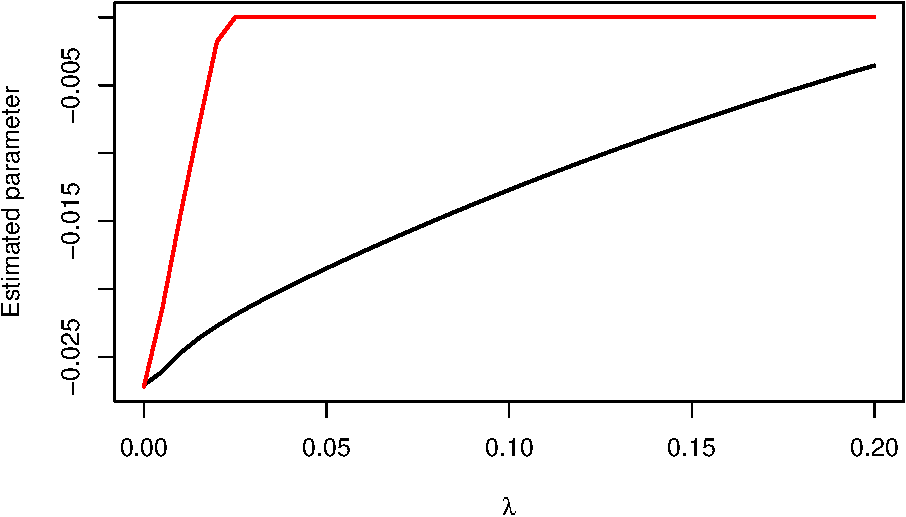
\includegraphics{EcoStat_files/figure-latex/lasso4-1.pdf}

Let us take two values of \(\lambda\) and see the associated estimated parameters in the context of lasso regressions:

\begin{Shaded}
\begin{Highlighting}[]
\NormalTok{i }\OtherTok{\textless{}{-}} \DecValTok{20}\NormalTok{; j }\OtherTok{\textless{}{-}} \DecValTok{40}
\FunctionTok{cbind}\NormalTok{(result.lasso}\SpecialCharTok{$}\NormalTok{lambda[i],result.lasso}\SpecialCharTok{$}\NormalTok{lambda[j])}
\end{Highlighting}
\end{Shaded}

\begin{verbatim}
##       [,1]  [,2]
## [1,] 0.105 0.005
\end{verbatim}

\begin{Shaded}
\begin{Highlighting}[]
\FunctionTok{cbind}\NormalTok{(}\FunctionTok{coef}\NormalTok{(result.lasso)[,i],}\FunctionTok{coef}\NormalTok{(result.lasso)[,j])}
\end{Highlighting}
\end{Shaded}

\begin{verbatim}
##                               [,1]          [,2]
## (Intercept)          -1.044971e-15  1.088731e-14
## delinq_2yrs           6.308870e-02  6.893527e-02
## annual_inc            0.000000e+00  4.595653e-03
## annual_inc2           0.000000e+00  0.000000e+00
## log_annual_inc        0.000000e+00 -3.612382e-02
## dti                   0.000000e+00  2.242246e-02
## installment           1.476796e-01  8.228729e+00
## verification_status   0.000000e+00 -9.750047e-04
## funded_amnt           0.000000e+00 -7.309169e+00
## funded_amnt2          0.000000e+00 -4.711846e-01
## log_funded_amnt       0.000000e+00 -2.460932e-01
## pub_rec               3.390816e-02  5.997252e-02
## emp_length_10         0.000000e+00 -1.924941e-02
## owner                 0.000000e+00 -2.444599e-02
## renter               -3.882640e-02 -6.243087e-02
## pub_rec_bankruptcies  0.000000e+00  0.000000e+00
## revol_util            0.000000e+00  0.000000e+00
## revol_bal             0.000000e+00  2.402268e-03
\end{verbatim}

\begin{Shaded}
\begin{Highlighting}[]
\CommentTok{\# Compute values of y predicted by the model, for all lambdas:}
\NormalTok{pred1 }\OtherTok{\textless{}{-}} \FunctionTok{predict}\NormalTok{(result.lasso,}\FunctionTok{as.matrix}\NormalTok{(x))}
\CommentTok{\# Compute values of y predicted by the model, for a specific value:}
\NormalTok{pred2 }\OtherTok{\textless{}{-}} \FunctionTok{predict}\NormalTok{(result.lasso,}\FunctionTok{as.matrix}\NormalTok{(x),}\AttributeTok{s=}\FloatTok{0.085}\NormalTok{)}
\end{Highlighting}
\end{Shaded}

The \texttt{glmnet} package (see \href{https://glmnet.stanford.edu/articles/glmnet.html}{Hastie et al.~(2021)}) also offers tools to implement cross-validation:

\begin{Shaded}
\begin{Highlighting}[]
\CommentTok{\# cross validation (cv):}
\NormalTok{cvglmnet }\OtherTok{\textless{}{-}} \FunctionTok{cv.glmnet}\NormalTok{(}\FunctionTok{as.matrix}\NormalTok{(x),y)}
\FunctionTok{plot}\NormalTok{(cvglmnet)}
\end{Highlighting}
\end{Shaded}

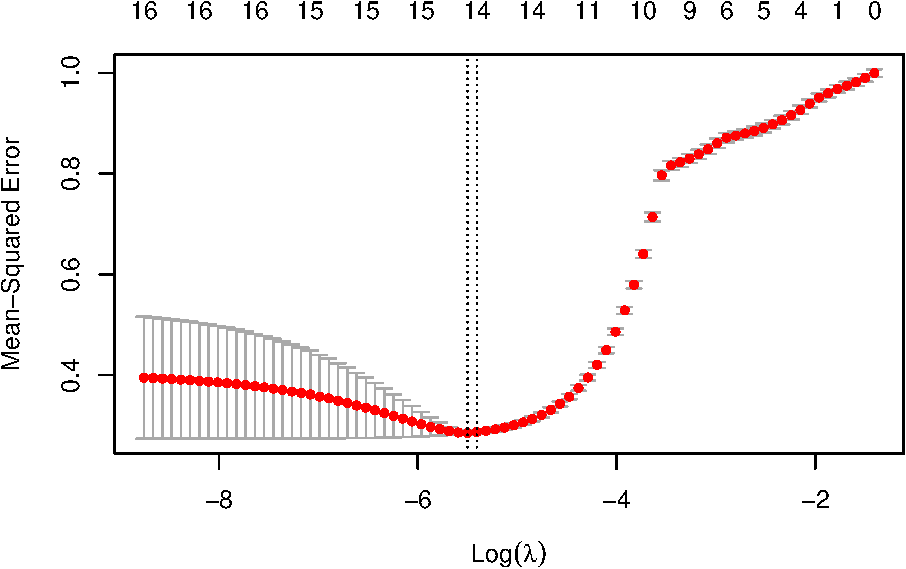
\includegraphics{EcoStat_files/figure-latex/lasso6-1.pdf}

\begin{Shaded}
\begin{Highlighting}[]
\CommentTok{\# lambda.min: lambda that gives minimum mean cross{-}validated error}
\NormalTok{cvglmnet}\SpecialCharTok{$}\NormalTok{lambda.min }
\end{Highlighting}
\end{Shaded}

\begin{verbatim}
## [1] 0.004091039
\end{verbatim}

\begin{Shaded}
\begin{Highlighting}[]
\CommentTok{\# lambda.1se: largest lambda s.t. cost within the one{-}std{-}dev cv{-}based band}
\NormalTok{cvglmnet}\SpecialCharTok{$}\NormalTok{lambda}\FloatTok{.1}\NormalTok{se}
\end{Highlighting}
\end{Shaded}

\begin{verbatim}
## [1] 0.00448991
\end{verbatim}

\begin{Shaded}
\begin{Highlighting}[]
\FunctionTok{coef}\NormalTok{(cvglmnet, }\AttributeTok{s =} \StringTok{"lambda.min"}\NormalTok{) }\CommentTok{\# associated parameters}
\end{Highlighting}
\end{Shaded}

\begin{verbatim}
## 18 x 1 sparse Matrix of class "dgCMatrix"
##                                 s1
## (Intercept)           1.128990e-14
## delinq_2yrs           6.625860e-02
## annual_inc            6.054923e-03
## annual_inc2           .           
## log_annual_inc       -3.795151e-02
## dti                   2.065272e-02
## installment           8.518961e+00
## verification_status  -2.894435e-03
## funded_amnt          -7.560853e+00
## funded_amnt2         -5.041923e-01
## log_funded_amnt      -2.537567e-01
## pub_rec               5.804333e-02
## emp_length_10        -1.894666e-02
## owner                -2.484192e-02
## renter               -6.039831e-02
## pub_rec_bankruptcies  .           
## revol_util            .           
## revol_bal             3.093752e-03
\end{verbatim}

\begin{Shaded}
\begin{Highlighting}[]
\CommentTok{\# predicted values of y for specific values of x:}
\FunctionTok{predict}\NormalTok{(cvglmnet, }\AttributeTok{newx =} \FunctionTok{as.matrix}\NormalTok{(x)[}\DecValTok{1}\SpecialCharTok{:}\DecValTok{5}\NormalTok{,], }\AttributeTok{s =} \StringTok{"lambda.min"}\NormalTok{) }
\end{Highlighting}
\end{Shaded}

\begin{verbatim}
##        lambda.min
## 21529  0.34496384
## 21547 -0.04553753
## 21579  0.56455499
## 21583 -0.20696954
## 21608 -0.12165356
\end{verbatim}

\hypertarget{Panel}{%
\chapter{Panel regressions}\label{Panel}}

\hypertarget{specification-and-notations}{%
\section{Specification and notations}\label{specification-and-notations}}

A standard panel situation is as follows: the sample covers a lot of ``entities'', indexed by \(i \in \{1,\dots,n\}\), with \(n\) large, and, for each entity, we observe different variables over a small number of periods \(t \in \{1,\dots,T\}\). This is a \emph{longitudinal dataset}.

The linear panel regression model is:
\begin{equation}
y_{i,t} = \mathbf{x}'_{i,t}\underbrace{\boldsymbol\beta}_{K \times 1} + \underbrace{\mathbf{z}'_{i}\boldsymbol\alpha}_{\mbox{Individual effects}} + \varepsilon_{i,t}.\label{eq:panel1}
\end{equation}

When running panel regressions, the usual objective is to estimate \(\boldsymbol\beta\).

Figure \ref{fig:simulPanel} illustrates a panel-data situation. The model is \(y_i = \alpha_i + \beta x_{i,t} + \varepsilon_{i,t}\), \(t \in \{1,2\}\). On Panel (b), blue dots are for \(t=1\), red dots are for \(t=2\). The lines relate the dots associated with the same entity \(i\). What is remarkable in the simulated model is that, while the unconditional correlation between \(y\) and \(x\) is negative, the conditional correlation (conditional on \(\alpha_i\)) is positive. Indeed, the sign of this conditional correlation is the sign of \(\beta\), which is positive in th simulated example (\(\beta=5\)). In other words, if one did not know the panel nature of the data, that would be tempting to say that \(\beta<0\), but this is not the case, due to \textbf{fixed effects} (the \(\alpha_i\)'s) that are negatively correlated to the \(x_i\)'s.

\begin{Shaded}
\begin{Highlighting}[]
\NormalTok{T }\OtherTok{\textless{}{-}} \DecValTok{2}\NormalTok{; n }\OtherTok{\textless{}{-}} \DecValTok{12} \CommentTok{\# 2 periods and 12 entities}
\NormalTok{alpha }\OtherTok{\textless{}{-}} \DecValTok{5}\SpecialCharTok{*}\FunctionTok{rnorm}\NormalTok{(n) }\CommentTok{\# draw fixed effects}
\NormalTok{x}\FloatTok{.1} \OtherTok{\textless{}{-}} \FunctionTok{rnorm}\NormalTok{(n) }\SpecialCharTok{{-}}\NormalTok{ .}\DecValTok{5}\SpecialCharTok{*}\NormalTok{alpha }\CommentTok{\# note: x\_i\textquotesingle{}s correlate to alpha\_i\textquotesingle{}s}
\NormalTok{x}\FloatTok{.2} \OtherTok{\textless{}{-}} \FunctionTok{rnorm}\NormalTok{(n) }\SpecialCharTok{{-}}\NormalTok{ .}\DecValTok{5}\SpecialCharTok{*}\NormalTok{alpha}
\NormalTok{beta }\OtherTok{\textless{}{-}} \DecValTok{5}\NormalTok{; sigma }\OtherTok{\textless{}{-}}\NormalTok{ .}\DecValTok{3}
\NormalTok{y}\FloatTok{.1} \OtherTok{\textless{}{-}}\NormalTok{ alpha }\SpecialCharTok{+}\NormalTok{ x}\FloatTok{.1} \SpecialCharTok{+}\NormalTok{ sigma}\SpecialCharTok{*}\FunctionTok{rnorm}\NormalTok{(n);y}\FloatTok{.2} \OtherTok{\textless{}{-}}\NormalTok{ alpha }\SpecialCharTok{+}\NormalTok{ x}\FloatTok{.2} \SpecialCharTok{+}\NormalTok{ sigma}\SpecialCharTok{*}\FunctionTok{rnorm}\NormalTok{(n)}
\NormalTok{x }\OtherTok{\textless{}{-}} \FunctionTok{c}\NormalTok{(x}\FloatTok{.1}\NormalTok{,x}\FloatTok{.2}\NormalTok{) }\CommentTok{\# pooled x}
\NormalTok{y }\OtherTok{\textless{}{-}} \FunctionTok{c}\NormalTok{(y}\FloatTok{.1}\NormalTok{,y}\FloatTok{.2}\NormalTok{) }\CommentTok{\# pooled y}
\FunctionTok{par}\NormalTok{(}\AttributeTok{mfrow=}\FunctionTok{c}\NormalTok{(}\DecValTok{1}\NormalTok{,}\DecValTok{2}\NormalTok{))}
\FunctionTok{plot}\NormalTok{(x,y,}\AttributeTok{col=}\StringTok{"black"}\NormalTok{,}\AttributeTok{pch=}\DecValTok{19}\NormalTok{,}\AttributeTok{xlab=}\StringTok{"x"}\NormalTok{,}\AttributeTok{ylab=}\StringTok{"y"}\NormalTok{,}\AttributeTok{main=}\StringTok{"(a)"}\NormalTok{)}
\FunctionTok{plot}\NormalTok{(x,y,}\AttributeTok{col=}\StringTok{"black"}\NormalTok{,}\AttributeTok{pch=}\DecValTok{19}\NormalTok{,}\AttributeTok{xlab=}\StringTok{"x"}\NormalTok{,}\AttributeTok{ylab=}\StringTok{"y"}\NormalTok{,}\AttributeTok{main=}\StringTok{"(b)"}\NormalTok{)}
\FunctionTok{points}\NormalTok{(x}\FloatTok{.1}\NormalTok{,y}\FloatTok{.1}\NormalTok{,}\AttributeTok{col=}\StringTok{"blue"}\NormalTok{,}\AttributeTok{pch=}\DecValTok{19}\NormalTok{);}\FunctionTok{points}\NormalTok{(x}\FloatTok{.2}\NormalTok{,y}\FloatTok{.2}\NormalTok{,}\AttributeTok{col=}\StringTok{"red"}\NormalTok{,}\AttributeTok{pch=}\DecValTok{19}\NormalTok{)}
\ControlFlowTok{for}\NormalTok{(i }\ControlFlowTok{in} \DecValTok{1}\SpecialCharTok{:}\NormalTok{n)\{}\FunctionTok{lines}\NormalTok{(}\FunctionTok{c}\NormalTok{(x}\FloatTok{.1}\NormalTok{[i],x}\FloatTok{.2}\NormalTok{[i]),}\FunctionTok{c}\NormalTok{(y}\FloatTok{.1}\NormalTok{[i],y}\FloatTok{.2}\NormalTok{[i]))\}}
\end{Highlighting}
\end{Shaded}

\begin{figure}
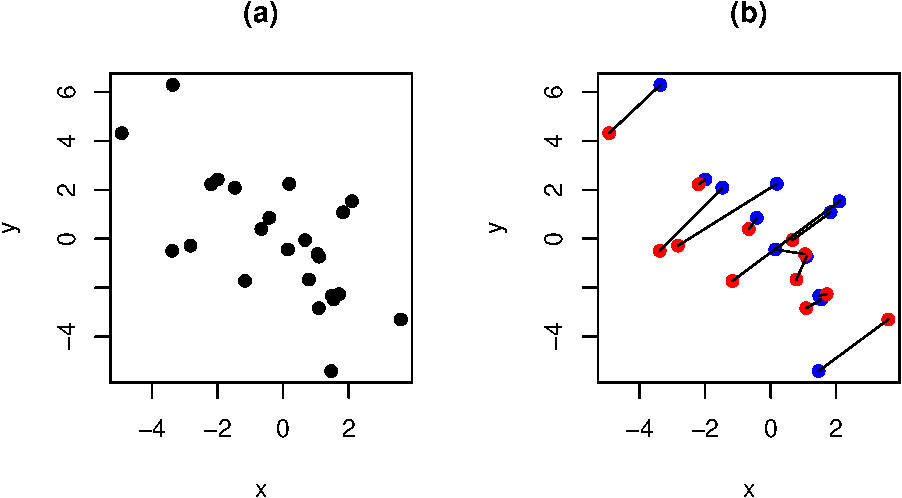
\includegraphics[width=0.95\linewidth]{EcoStat_files/figure-latex/simulPanel-1} \caption{The data are the same for both panels. On Panel (b), blue dots are for $t=1$, red dots are for $t=2$. The lines relate the dots associated to the same entity $i$.}\label{fig:simulPanel}
\end{figure}

Figure \ref{fig:cigarettes} presents the same type of plot based on the Cigarette Consumption Panel dataset (\texttt{CigarettesSW} dataset, used in \citet{Stock_Watson_2003}). This dataset documents the average consumption of cigarettes in 48 continental US states for two dates (1985 and 1995).

\begin{figure}
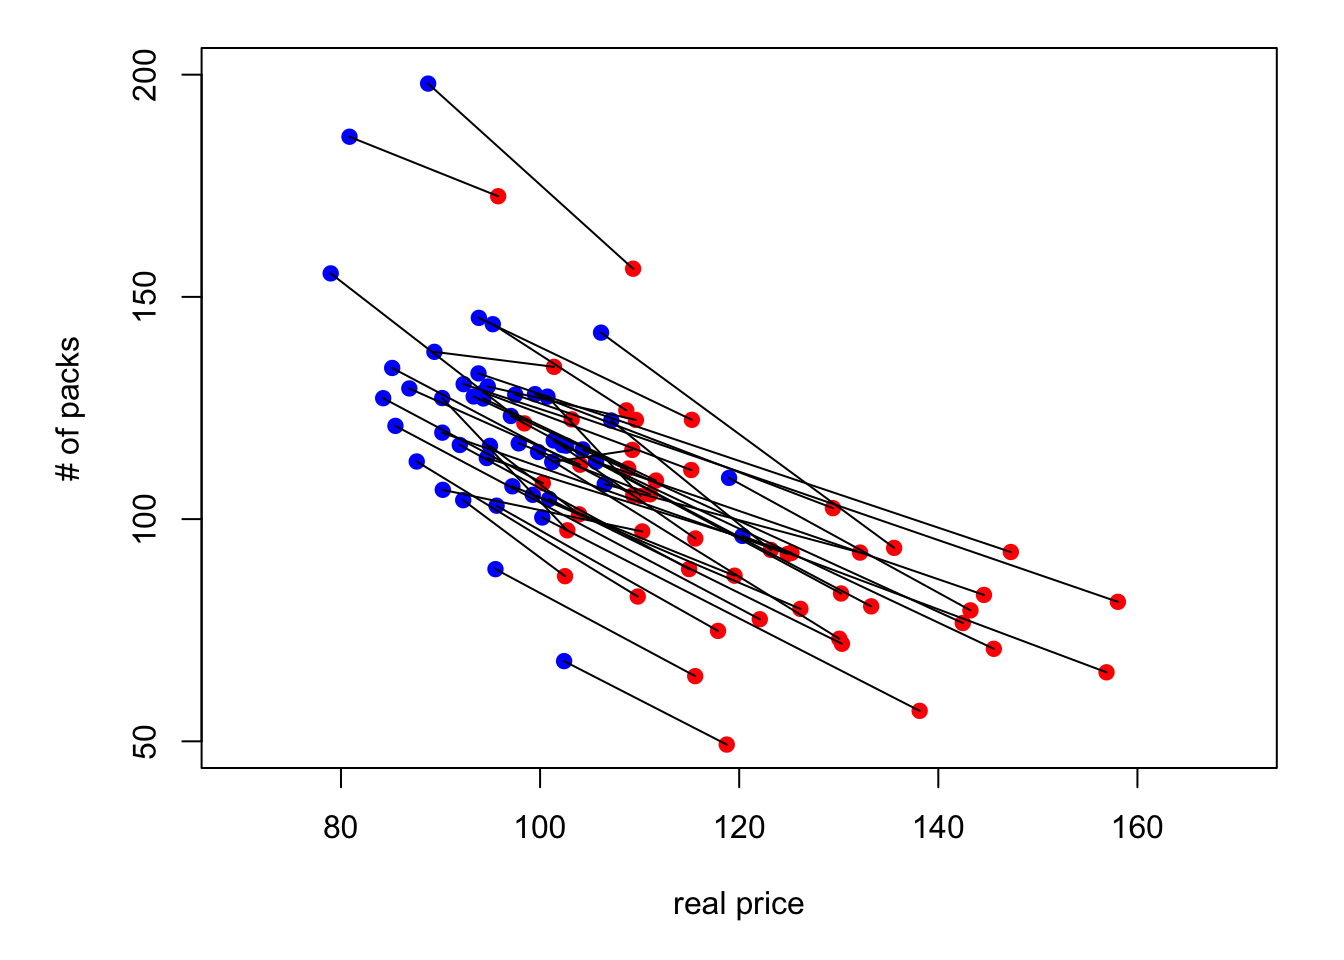
\includegraphics[width=0.95\linewidth]{EcoStat_files/figure-latex/cigarettes-1} \caption{Cigarette consumption versus real price in the CigarettesSW panel dataset.}\label{fig:cigarettes}
\end{figure}

We will make use of the following notations:
\[
\mathbf{y}_i =
\underbrace{\left[
\begin{array}{c}
y_{i,1}\\
\vdots\\
y_{i,T}
\end{array}\right]}_{T \times 1}, \quad
\boldsymbol\varepsilon_i =
\underbrace{\left[
\begin{array}{c}
\varepsilon_{i,1}\\
\vdots\\
\varepsilon_{i,T}
\end{array}\right]}_{T \times 1}, \quad
\mathbf{x}_i =
\underbrace{\left[
\begin{array}{c}
\mathbf{x}_{i,1}'\\
\vdots\\
\mathbf{x}_{i,T}'
\end{array}\right]}_{T \times K}, \quad
\mathbf{X} =
\underbrace{\left[
\begin{array}{c}
\mathbf{x}_{1}\\
\vdots\\
\mathbf{x}_{n}
\end{array}\right]}_{(nT) \times K}.
\]
\[
\tilde{\mathbf{y}}_i =
\left[
\begin{array}{c}
y_{i,1} - \bar{y}_i\\
\vdots\\
y_{i,T} - \bar{y}_i
\end{array}\right], \quad
\tilde{\boldsymbol\varepsilon}_i =
\left[
\begin{array}{c}
\varepsilon_{i,1} - \bar{\varepsilon}_i\\
\vdots\\
\varepsilon_{i,T} - \bar{\varepsilon}_i
\end{array}\right],
\]
\[
\tilde{\mathbf{x}}_i =
\left[
\begin{array}{c}
\mathbf{x}_{i,1}' - \bar{\mathbf{x}}_i'\\
\vdots\\
\mathbf{x}_{i,T}' - \bar{\mathbf{x}}_i'
\end{array}\right], \quad
\tilde{\mathbf{X}} =
\left[
\begin{array}{c}
\tilde{\mathbf{x}}_{1}\\
\vdots\\
\tilde{\mathbf{x}}_{n}
\end{array}\right], \quad
\tilde{\mathbf{Y}} =
\left[
\begin{array}{c}
\tilde{\mathbf{y}}_{1}\\
\vdots\\
\tilde{\mathbf{y}}_{n}
\end{array}\right],
\]
where
\[
\bar{y}_i = \frac{1}{T} \sum_{t=1}^T y_{i,t}, \quad \bar{\varepsilon}_i = \frac{1}{T}\sum_{t=1}^T \varepsilon_{i,t} \quad \mbox{and} \quad \bar{\mathbf{x}}_i = \frac{1}{T}\sum_{t=1}^T \mathbf{x}_{i,t}.
\]

\hypertarget{three-standard-cases}{%
\section{Three standard cases}\label{three-standard-cases}}

There are three typical situations:

\begin{itemize}
\tightlist
\item
  \textbf{Pooled regression}: \(\mathbf{z}_i \equiv 1\). This case amounts to the case studied in Chapter \ref{ChapterLS}.
\item
  \textbf{Fixed Effects} (Section \ref{FixedEffect}): \(\mathbf{z}_i\) is unobserved, but correlates with \(\mathbf{x}_i\) \(\Rightarrow\) \(\mathbf{b}\) is biased and inconsistent in the OLS regression of \(\mathbf{y}\) on \(\mathbf{X}\) (omitted variable, see Section \ref{Omitted}).
\item
  \textbf{Random Effects} (Section \ref{RandomEffect}): \(\mathbf{z}_i\) is unobserved, but uncorrelated with \(\mathbf{x}_i\). The model writes:
  \[
  y_{i,t} = \mathbf{x}'_{i,t}\boldsymbol\beta + \alpha +  \underbrace{{\color{blue}u_i + \varepsilon_{i,t}}}_{\mbox{compound error}},
  \]
  where \(\alpha = \mathbb{E}(\mathbf{z}'_{i}\boldsymbol\alpha)\) and \(u_i = \mathbf{z}'_{i}\boldsymbol\alpha - \mathbb{E}(\mathbf{z}'_{i}\boldsymbol\alpha) \perp \mathbf{x}_i\). In that case, the OLS is consistent, but not efficient. GLS can be used to gain efficiencies over OLS (see Section \ref{GLS} for a presentation of the GLS approach).
\end{itemize}

\hypertarget{FixedEffect}{%
\section{Estimation of Fixed-Effects Models}\label{FixedEffect}}

\begin{hypothesis}[Fixed-effect model]
\protect\hypertarget{hyp:FE}{}\label{hyp:FE}

We assume that:

\begin{enumerate}
\def\labelenumi{\roman{enumi}.}
\tightlist
\item
  There is no perfect multicollinearity among the regressors.
\item
  \(\mathbb{E}(\varepsilon_{i,t}|\mathbf{X})=0\), for all \(i,t\).
\item
  We have:
  \[
  \mathbb{E}(\varepsilon_{i,t}\varepsilon_{j,s}|\mathbf{X}) =
  \left\{
  \begin{array}{cl}
  \sigma^2 & \mbox{if $i=j$ and $s=t$},\\
  0 & \mbox{otherwise.}
  \end{array}\right.
  \]
\end{enumerate}

\end{hypothesis}

These assumptions are analogous to those introduced in the standard linear regression:

\begin{enumerate}
\def\labelenumi{(\roman{enumi})}
\tightlist
\item
  \(\leftrightarrow\) Hyp. \ref{hyp:fullrank}, (ii) \(\leftrightarrow\) Hyp. \ref{hyp:exogeneity}, (iii) \(\leftrightarrow\) Hyp. \ref{hyp:homoskedasticity} + \ref{hyp:noncorrelResid}.
\end{enumerate}

In matrix form, for a given \(i\), the model writes:
\[
\mathbf{y}_i = \mathbf{x}_i \boldsymbol\beta + \mathbf{1}\alpha_i + \boldsymbol\varepsilon_i,
\]
where \(\mathbf{1}\) is a \(T\)-dimensional vector of ones.

This is the \textbf{Least Square Dummy Variable (LSDV)} model:
\begin{equation}
\mathbf{y} = [\mathbf{X} \quad \mathbf{D}]
\left[
\begin{array}{c}
\boldsymbol\beta\\
\boldsymbol\alpha
\end{array}
\right]
+ \boldsymbol\varepsilon, \label{eq:LSDV}
\end{equation}
with:
\[
\mathbf{D} = \underbrace{ \left[\begin{array}{cccc}
\mathbf{1}&\mathbf{0}&\dots&\mathbf{0}\\
\mathbf{0}&\mathbf{1}&\dots&\mathbf{0}\\
&&\vdots&\\
\mathbf{0}&\mathbf{0}&\dots&\mathbf{1}\\
\end{array}\right]}_{(nT \times n)}.
\]

The linear regression (Eq. \eqref{eq:LSDV}) ---with the dummy variables--- satisfies the Gauss-Markov conditions (Theorem \ref{thm:GaussMarkov}). Hence, in this context, the OLS estimator is the \emph{best linear unbiased estimator} (BLUE).

Denoting by \(\mathbf{Z}\) the matrix \([\mathbf{X} \quad \mathbf{D}]\), and by \(\mathbf{b}\) and \(\mathbf{a}\) the respective OLS estimates of \(\boldsymbol\beta\) and of \(\boldsymbol\alpha\), we have:
\begin{equation}
\boxed{
\left[
\begin{array}{c}
\mathbf{b}\\
\mathbf{a}
\end{array}
\right]
= [\mathbf{Z}'\mathbf{Z}]^{-1}\mathbf{Z}'\mathbf{y}.} \label{eq:bfixedeffects11}
\end{equation}

The asymptotical distribution of \([\mathbf{b}',\mathbf{a}']'\) derives from the standard OLS context: Prop. \ref{prp:asymptOLS} can be used after having replaced \(\mathbf{X}\) by \(\mathbf{Z}=[\mathbf{X} \quad \mathbf{D}]\).

We have:
\begin{equation}
\boxed{\left[
\begin{array}{c}
\mathbf{b}\\
\mathbf{a}
\end{array}
\right] \overset{d}{\rightarrow}
\mathcal{N}\left(
\left[
\begin{array}{c}
\boldsymbol\beta\\
\boldsymbol\alpha
\end{array}
\right],
\sigma^2 \frac{Q^{-1}}{nT}
\right),}
\end{equation}
where
\[
Q = \mbox{plim}_{nT \rightarrow \infty} \frac{1}{nT} \mathbf{Z}'\mathbf{Z},
\]
assuming the previous limit exists.

In practice, an estimator of the covariance matrix of \([\mathbf{b}',\mathbf{a}']'\) is:
\[
s^2 \left( \mathbf{Z}'\mathbf{Z}\right)^{-1} \quad with \quad s^2 = \frac{\mathbf{e}'\mathbf{e}}{nT - K - n},
\]
where \(\mathbf{e}\) is the \((nT) \times 1\) vector of OLS residuals.

There is an alternative way of expressing the LSDV estimators. It involves the residual-maker matrix matrix \(\mathbf{M_D}=\mathbf{I} - \mathbf{D}(\mathbf{D}'\mathbf{D})^{-1}\mathbf{D}'\) (see Eq. \eqref{eq:Mres}), which acts as an operator that removes entity-specific means, i.e.:
\[
\tilde{\mathbf{Y}} = \mathbf{M_D}\mathbf{Y}, \quad \tilde{\mathbf{X}} = \mathbf{M_D}\mathbf{X} \quad and \quad \tilde{\boldsymbol\varepsilon} = \mathbf{M_D}\boldsymbol\varepsilon.
\]

With these notations, using the Frisch-Waugh theorem (Theorem \ref{thm:FW}), we get another expression for the estimator \(\mathbf{b}\) appearing in Eq. \eqref{eq:bfixedeffects11}:
\begin{equation}
\boxed{\mathbf{b} = [\mathbf{X}'\mathbf{M_D}\mathbf{X}]^{-1}\mathbf{X}'\mathbf{M_D}\mathbf{y}.}\label{eq:bfixedeffects}
\end{equation}

This amounts to regressing the \(\tilde{y}_{i,t}\)'s (\(= y_{i,t} - \bar{y}_i\)) on the \(\tilde{\mathbf{x}}_{i,t}\)'s (\(=\mathbf{x}_{i,t} - \bar{\mathbf{x}}_i\)).

The estimate of \(\boldsymbol\alpha\) is given by:
\begin{equation}
\boxed{\mathbf{a} = (\mathbf{D}'\mathbf{D})^{-1}\mathbf{D}'(\mathbf{y} - \mathbf{X}\mathbf{b}),} \label{eq:a}
\end{equation}
which is obtained by developing the second row of
\[
\left[
\begin{array}{cc}
\mathbf{X}'\mathbf{X} & \mathbf{X}'\mathbf{D}\\
\mathbf{D}'\mathbf{X} & \mathbf{D}'\mathbf{D}
\end{array}\right]
\left[
\begin{array}{c}
\mathbf{b}\\
\mathbf{a}
\end{array}\right] =
\left[
\begin{array}{c}
\mathbf{X}'\mathbf{Y}\\
\mathbf{D}'\mathbf{Y}
\end{array}\right],
\]
which are the first-order conditions resulting from the least squares problem (see Eq. \eqref{eq:OLSFOC}).

One can use different types of fixed effects in the same regression. Typically, one can have time and entity fixed effects. In that case, the model writes:
\[
y_{i,t} = \mathbf{x}_i'\boldsymbol\beta + \alpha_i + \gamma_t + \varepsilon_{i,t}.
\]

The LSDV approach (Eq. \eqref{eq:LSDV}) can still be resorted to. It suffices to extend the \(\mathbf{Z}\) matrix with additional columns (then called \emph{time dummies}):
\begin{equation}
\mathbf{y} = [\mathbf{X} \quad \mathbf{D} \quad \mathbf{C}]
\left[
\begin{array}{c}
\boldsymbol\beta\\
\boldsymbol\alpha\\
\boldsymbol\gamma
\end{array}
\right]
+ \boldsymbol\varepsilon, \label{eq:LSDV2}
\end{equation}
with:
\[
\mathbf{C} = \left[\begin{array}{cccc}
\boldsymbol{\delta}_1&\boldsymbol{\delta}_2&\dots&\boldsymbol{\delta}_{T-1}\\
\vdots&\vdots&&\vdots\\
\boldsymbol{\delta}_1&\boldsymbol{\delta}_2&\dots&\boldsymbol{\delta}_{T-1}\\
\end{array}\right],
\]
where the \(T\)-dimensional vector \(\boldsymbol\delta_t\) (the \emph{time dummy}) is
\[
[0,\dots,0,\underbrace{1}_{\mbox{t$^{th}$ entry}},0,\dots,0]'.
\]

Using state and year fixed effects in the \texttt{CigarettesSW} panel dataset yields the following results:

\begin{Shaded}
\begin{Highlighting}[]
\NormalTok{CigarettesSW}\SpecialCharTok{$}\NormalTok{rincome }\OtherTok{\textless{}{-}} \FunctionTok{with}\NormalTok{(CigarettesSW, income}\SpecialCharTok{/}\NormalTok{population}\SpecialCharTok{/}\NormalTok{cpi)}
\NormalTok{eq.pooled }\OtherTok{\textless{}{-}} \FunctionTok{lm}\NormalTok{(}\FunctionTok{log}\NormalTok{(packs)}\SpecialCharTok{\textasciitilde{}}\FunctionTok{log}\NormalTok{(rprice)}\SpecialCharTok{+}\FunctionTok{log}\NormalTok{(rincome),}\AttributeTok{data=}\NormalTok{CigarettesSW)}
\NormalTok{eq.LSDV }\OtherTok{\textless{}{-}} \FunctionTok{lm}\NormalTok{(}\FunctionTok{log}\NormalTok{(packs)}\SpecialCharTok{\textasciitilde{}}\FunctionTok{log}\NormalTok{(rprice)}\SpecialCharTok{+}\FunctionTok{log}\NormalTok{(rincome)}\SpecialCharTok{+}\NormalTok{state,}
              \AttributeTok{data=}\NormalTok{CigarettesSW)}
\NormalTok{CigarettesSW}\SpecialCharTok{$}\NormalTok{year }\OtherTok{\textless{}{-}} \FunctionTok{as.factor}\NormalTok{(CigarettesSW}\SpecialCharTok{$}\NormalTok{year)}
\NormalTok{eq.LSDV2 }\OtherTok{\textless{}{-}} \FunctionTok{lm}\NormalTok{(}\FunctionTok{log}\NormalTok{(packs)}\SpecialCharTok{\textasciitilde{}}\FunctionTok{log}\NormalTok{(rprice)}\SpecialCharTok{+}\FunctionTok{log}\NormalTok{(rincome)}\SpecialCharTok{+}\NormalTok{state}\SpecialCharTok{+}\NormalTok{year,}
               \AttributeTok{data=}\NormalTok{CigarettesSW)}
\NormalTok{stargazer}\SpecialCharTok{::}\FunctionTok{stargazer}\NormalTok{(eq.pooled,eq.LSDV,eq.LSDV2,}\AttributeTok{type=}\StringTok{"text"}\NormalTok{,}\AttributeTok{no.space =} \ConstantTok{TRUE}\NormalTok{,}
                     \AttributeTok{omit=}\FunctionTok{c}\NormalTok{(}\StringTok{"state"}\NormalTok{,}\StringTok{"year"}\NormalTok{),}
                     \AttributeTok{add.lines=}\FunctionTok{list}\NormalTok{(}\FunctionTok{c}\NormalTok{(}\StringTok{\textquotesingle{}State FE\textquotesingle{}}\NormalTok{,}\StringTok{\textquotesingle{}No\textquotesingle{}}\NormalTok{,}\StringTok{\textquotesingle{}Yes\textquotesingle{}}\NormalTok{,}\StringTok{\textquotesingle{}Yes\textquotesingle{}}\NormalTok{),}
                                    \FunctionTok{c}\NormalTok{(}\StringTok{\textquotesingle{}Year FE\textquotesingle{}}\NormalTok{,}\StringTok{\textquotesingle{}No\textquotesingle{}}\NormalTok{,}\StringTok{\textquotesingle{}No\textquotesingle{}}\NormalTok{,}\StringTok{\textquotesingle{}Yes\textquotesingle{}}\NormalTok{)),}
                     \AttributeTok{omit.stat=}\FunctionTok{c}\NormalTok{(}\StringTok{"f"}\NormalTok{,}\StringTok{"ser"}\NormalTok{))}
\end{Highlighting}
\end{Shaded}

\begin{verbatim}
## 
## ==========================================
##                   Dependent variable:     
##              -----------------------------
##                       log(packs)          
##                 (1)       (2)       (3)   
## ------------------------------------------
## log(rprice)  -1.334*** -1.210*** -1.056***
##               (0.135)   (0.114)   (0.149) 
## log(rincome)  0.318**    0.121     0.497  
##               (0.136)   (0.190)   (0.304) 
## Constant     10.067*** 9.954***  8.360*** 
##               (0.516)   (0.264)   (1.049) 
## ------------------------------------------
## State FE        No        Yes       Yes   
## Year FE         No        No        Yes   
## Observations    96        96        96    
## R2             0.552     0.966     0.967  
## Adjusted R2    0.542     0.929     0.931  
## ==========================================
## Note:          *p<0.1; **p<0.05; ***p<0.01
\end{verbatim}

\begin{example}[Housing prices and interest rates]
\protect\hypertarget{exm:JSTPanel}{}\label{exm:JSTPanel}

In this example, we want to estimate the effect of short and long-term interest rate on housing prices. The data come from the \citet{JST_2017} dataset (\href{https://www.macrohistory.net}{see this website}).

\begin{Shaded}
\begin{Highlighting}[]
\FunctionTok{library}\NormalTok{(AEC);}\FunctionTok{library}\NormalTok{(sandwich)}
\FunctionTok{data}\NormalTok{(JST); JST }\OtherTok{\textless{}{-}} \FunctionTok{subset}\NormalTok{(JST,year}\SpecialCharTok{\textgreater{}}\DecValTok{1950}\NormalTok{);N }\OtherTok{\textless{}{-}} \FunctionTok{dim}\NormalTok{(JST)[}\DecValTok{1}\NormalTok{]}
\NormalTok{JST}\SpecialCharTok{$}\NormalTok{hpreal }\OtherTok{\textless{}{-}}\NormalTok{ JST}\SpecialCharTok{$}\NormalTok{hpnom}\SpecialCharTok{/}\NormalTok{JST}\SpecialCharTok{$}\NormalTok{cpi }\CommentTok{\# real house price index}
\NormalTok{JST}\SpecialCharTok{$}\NormalTok{dhpreal }\OtherTok{\textless{}{-}} \DecValTok{100}\SpecialCharTok{*}\FunctionTok{log}\NormalTok{(JST}\SpecialCharTok{$}\NormalTok{hpreal}\SpecialCharTok{/}\FunctionTok{c}\NormalTok{(}\ConstantTok{NaN}\NormalTok{,JST}\SpecialCharTok{$}\NormalTok{hpreal[}\DecValTok{1}\SpecialCharTok{:}\NormalTok{(N}\DecValTok{{-}1}\NormalTok{)]))}
\CommentTok{\# Put NA\textquotesingle{}s when change in country:}
\NormalTok{JST}\SpecialCharTok{$}\NormalTok{dhpreal[}\FunctionTok{c}\NormalTok{(}\DecValTok{0}\NormalTok{,JST}\SpecialCharTok{$}\NormalTok{iso[}\DecValTok{2}\SpecialCharTok{:}\NormalTok{N]}\SpecialCharTok{!=}\NormalTok{JST}\SpecialCharTok{$}\NormalTok{iso[}\DecValTok{1}\SpecialCharTok{:}\NormalTok{(N}\DecValTok{{-}1}\NormalTok{)])] }\OtherTok{\textless{}{-}} \ConstantTok{NaN}
\NormalTok{JST}\SpecialCharTok{$}\NormalTok{dhpreal[}\FunctionTok{abs}\NormalTok{(JST}\SpecialCharTok{$}\NormalTok{dhpreal)}\SpecialCharTok{\textgreater{}}\DecValTok{30}\NormalTok{] }\OtherTok{\textless{}{-}} \ConstantTok{NaN} \CommentTok{\# remove extreme price change}
\NormalTok{JST}\SpecialCharTok{$}\NormalTok{YEAR }\OtherTok{\textless{}{-}} \FunctionTok{as.factor}\NormalTok{(JST}\SpecialCharTok{$}\NormalTok{year) }\CommentTok{\# to have time fixed effects}
\NormalTok{eq1\_noFE }\OtherTok{\textless{}{-}} \FunctionTok{lm}\NormalTok{(dhpreal }\SpecialCharTok{\textasciitilde{}}\NormalTok{ stir }\SpecialCharTok{+}\NormalTok{ ltrate,}\AttributeTok{data=}\NormalTok{JST)}
\NormalTok{eq1\_FE   }\OtherTok{\textless{}{-}} \FunctionTok{lm}\NormalTok{(dhpreal }\SpecialCharTok{\textasciitilde{}}\NormalTok{ stir }\SpecialCharTok{+}\NormalTok{ ltrate }\SpecialCharTok{+}\NormalTok{ iso }\SpecialCharTok{+}\NormalTok{ YEAR,}\AttributeTok{data=}\NormalTok{JST)}
\NormalTok{eq2\_noFE }\OtherTok{\textless{}{-}} \FunctionTok{lm}\NormalTok{(dhpreal }\SpecialCharTok{\textasciitilde{}} \FunctionTok{I}\NormalTok{(ltrate}\SpecialCharTok{{-}}\NormalTok{stir),}\AttributeTok{data=}\NormalTok{JST)}
\NormalTok{eq2\_FE }\OtherTok{\textless{}{-}} \FunctionTok{lm}\NormalTok{(dhpreal }\SpecialCharTok{\textasciitilde{}} \FunctionTok{I}\NormalTok{(ltrate}\SpecialCharTok{{-}}\NormalTok{stir) }\SpecialCharTok{+}\NormalTok{ iso }\SpecialCharTok{+}\NormalTok{ YEAR,}\AttributeTok{data=}\NormalTok{JST)}
\NormalTok{vcov\_cluster1\_noFE }\OtherTok{\textless{}{-}} \FunctionTok{vcovHC}\NormalTok{(eq1\_noFE, }\AttributeTok{cluster =}\NormalTok{ JST[, }\FunctionTok{c}\NormalTok{(}\StringTok{"iso"}\NormalTok{,}\StringTok{"YEAR"}\NormalTok{)])}
\NormalTok{vcov\_cluster1\_FE   }\OtherTok{\textless{}{-}} \FunctionTok{vcovHC}\NormalTok{(eq1\_FE, }\AttributeTok{cluster =}\NormalTok{ JST[, }\FunctionTok{c}\NormalTok{(}\StringTok{"iso"}\NormalTok{,}\StringTok{"YEAR"}\NormalTok{)])}
\NormalTok{vcov\_cluster2\_noFE }\OtherTok{\textless{}{-}} \FunctionTok{vcovHC}\NormalTok{(eq2\_noFE, }\AttributeTok{cluster =}\NormalTok{ JST[, }\FunctionTok{c}\NormalTok{(}\StringTok{"iso"}\NormalTok{,}\StringTok{"YEAR"}\NormalTok{)])}
\NormalTok{vcov\_cluster2\_FE   }\OtherTok{\textless{}{-}} \FunctionTok{vcovHC}\NormalTok{(eq2\_FE, }\AttributeTok{cluster =}\NormalTok{ JST[, }\FunctionTok{c}\NormalTok{(}\StringTok{"iso"}\NormalTok{,}\StringTok{"YEAR"}\NormalTok{)])}
\NormalTok{robust\_se\_FE1\_noFE }\OtherTok{\textless{}{-}} \FunctionTok{sqrt}\NormalTok{(}\FunctionTok{diag}\NormalTok{(vcov\_cluster1\_noFE))}
\NormalTok{robust\_se\_FE1\_FE   }\OtherTok{\textless{}{-}} \FunctionTok{sqrt}\NormalTok{(}\FunctionTok{diag}\NormalTok{(vcov\_cluster1\_FE))}
\NormalTok{robust\_se\_FE2\_noFE }\OtherTok{\textless{}{-}} \FunctionTok{sqrt}\NormalTok{(}\FunctionTok{diag}\NormalTok{(vcov\_cluster2\_noFE))}
\NormalTok{robust\_se\_FE2\_FE   }\OtherTok{\textless{}{-}} \FunctionTok{sqrt}\NormalTok{(}\FunctionTok{diag}\NormalTok{(vcov\_cluster2\_FE))}
\NormalTok{stargazer}\SpecialCharTok{::}\FunctionTok{stargazer}\NormalTok{(eq1\_noFE, eq1\_FE, eq2\_noFE, eq2\_FE, }\AttributeTok{type =} \StringTok{"text"}\NormalTok{,}
                     \AttributeTok{column.labels =} \FunctionTok{c}\NormalTok{(}\StringTok{"no FE"}\NormalTok{, }\StringTok{"with FE"}\NormalTok{, }\StringTok{"no FE"}\NormalTok{,}\StringTok{"with FE"}\NormalTok{),}
                     \AttributeTok{omit =} \FunctionTok{c}\NormalTok{(}\StringTok{"iso"}\NormalTok{,}\StringTok{"YEAR"}\NormalTok{,}\StringTok{"Constant"}\NormalTok{),}\AttributeTok{keep.stat =} \StringTok{"n"}\NormalTok{,}
                     \AttributeTok{add.lines=}\FunctionTok{list}\NormalTok{(}\FunctionTok{c}\NormalTok{(}\StringTok{\textquotesingle{}Country FE\textquotesingle{}}\NormalTok{,}\StringTok{\textquotesingle{}No\textquotesingle{}}\NormalTok{,}\StringTok{\textquotesingle{}Yes\textquotesingle{}}\NormalTok{,}\StringTok{\textquotesingle{}No\textquotesingle{}}\NormalTok{,}\StringTok{\textquotesingle{}Yes\textquotesingle{}}\NormalTok{),}
                                    \FunctionTok{c}\NormalTok{(}\StringTok{\textquotesingle{}Year FE\textquotesingle{}}\NormalTok{,}\StringTok{\textquotesingle{}No\textquotesingle{}}\NormalTok{,}\StringTok{\textquotesingle{}Yes\textquotesingle{}}\NormalTok{,}\StringTok{\textquotesingle{}No\textquotesingle{}}\NormalTok{,}\StringTok{\textquotesingle{}Yes\textquotesingle{}}\NormalTok{)),}
                     \AttributeTok{se =} \FunctionTok{list}\NormalTok{(robust\_se\_FE1\_noFE,robust\_se\_FE1\_FE,}
\NormalTok{                               robust\_se\_FE2\_noFE,robust\_se\_FE2\_FE))}
\end{Highlighting}
\end{Shaded}

\begin{verbatim}
## 
## =======================================================
##                           Dependent variable:          
##                  --------------------------------------
##                                 dhpreal                
##                    no FE   with FE    no FE    with FE 
##                     (1)      (2)       (3)       (4)   
## -------------------------------------------------------
## stir             0.485***  0.532***                    
##                   (0.149)  (0.170)                     
##                                                        
## ltrate           -0.690*** -0.384**                    
##                   (0.164)  (0.182)                     
##                                                        
## I(ltrate - stir)                    -0.476*** -0.475***
##                                      (0.145)   (0.159) 
##                                                        
## -------------------------------------------------------
## Country FE          No       Yes       No        Yes   
## Year FE             No       Yes       No        Yes   
## Observations       1,141    1,141     1,141     1,141  
## =======================================================
## Note:                       *p<0.1; **p<0.05; ***p<0.01
\end{verbatim}

\end{example}

\hypertarget{RandomEffect}{%
\section{Estimation of random effects models}\label{RandomEffect}}

Here, the individual effects are assumed to be not correlated to other variables (the \(\mathbf{x}_i\)'s). In that context, the OLS estimator is consistent. However, it is not efficient. The GLS approach can be employed to gain efficiency.

\textbf{Random-effect models} write:
\[
y_{i,t}=\mathbf{x}'_{it}\boldsymbol\beta + (\alpha + \underbrace{u_i}_{\substack{\text{Random}\\\text{heterogeneity}}}) + \varepsilon_{i,t},
\]
with
\begin{eqnarray*}
\mathbb{E}(\varepsilon_{i,t}|\mathbf{X})&=&\mathbb{E}(u_{i}|\mathbf{X}) =0,\\
\mathbb{E}(\varepsilon_{i,t}\varepsilon_{j,s}|\mathbf{X}) &=&
\left\{
\begin{array}{cl}
\sigma_\varepsilon^2 & \mbox{ if $i=j$ and $s=t$},\\
0 & \mbox{ otherwise.}
\end{array}
\right.\\
\mathbb{E}(u_{i}u_{j}|\mathbf{X}) &=&
\left\{
\begin{array}{cl}
\sigma_u^2 & \mbox{ if $i=j$},\\
0 & \mbox{otherwise.}
\end{array}
\right.\\
\mathbb{E}(\varepsilon_{i,t}u_{j}|\mathbf{X})&=&0 \quad \text{for all $i$, $j$ and $t$}.
\end{eqnarray*}

Introducing the notations \(\eta_{i,t} = u_i + \varepsilon_{i,t}\) and \(\boldsymbol\eta_i = [\eta_{i,1},\dots,\eta_{i,T}]'\), we have \(\mathbb{E}(\boldsymbol\eta_i |\mathbf{X}) = \mathbf{0}\) and \(\mathbb{V}ar(\boldsymbol\eta_i | \mathbf{X}) = \boldsymbol\Gamma\), where
\[
\boldsymbol\Gamma = \left[  \begin{array}{ccccc}
\sigma_\varepsilon^2+\sigma_u^2 & \sigma_u^2 & \sigma_u^2 & \dots & \sigma_u^2\\
\sigma_u^2 & \sigma_\varepsilon^2+\sigma_u^2 & \sigma_u^2 & \dots & \sigma_u^2\\
\vdots && \ddots && \vdots \\
\sigma_u^2 & \sigma_u^2 & \sigma_u^2 & \dots & \sigma_\varepsilon^2+\sigma_u^2\\
\end{array}
\right] = \sigma_\varepsilon^2\mathbf{I} + \sigma_u^2\mathbf{1}\mathbf{1}'.
\]

Denoting by \(\boldsymbol\Sigma\) the covariance matrix of \(\boldsymbol\eta = [\boldsymbol\eta_1',\dots,\boldsymbol\eta_n']'\), we have:
\[
\boldsymbol\Sigma = \mathbf{I} \otimes \boldsymbol\Gamma.
\]

If we knew \(\boldsymbol\Sigma\), we would apply (feasible) GLS (Eq. \eqref{eq:betaGLS}, in Section \ref{GLS}):
\[
\boldsymbol\beta = (\mathbf{X}'\boldsymbol\Sigma^{-1}\mathbf{X})^{-1}\mathbf{X}'\boldsymbol\Sigma^{-1}\mathbf{y}.
\]
(As explained in Section \ref{GLS}, this amounts to regressing \({\boldsymbol\Sigma^{-1/2}}'\mathbf{y}\) on \({\boldsymbol\Sigma^{-1/2}}'\mathbf{X}\).)

It can be checked that \(\boldsymbol\Sigma^{-1/2} = \mathbf{I} \otimes (\boldsymbol\Gamma^{-1/2})\) where
\[
\boldsymbol\Gamma^{-1/2} = \frac{1}{\sigma_\varepsilon}\left( \mathbf{I} - \frac{\theta}{T}\mathbf{1}\mathbf{1}'\right),\quad \mbox{with}\quad\theta = 1 - \frac{\sigma_\varepsilon}{\sqrt{\sigma_\varepsilon^2+T\sigma_u^2}}.
\]

Hence, if we knew \(\boldsymbol\Sigma\), we would transform the data as follows:
\[
\boldsymbol\Gamma^{-1/2}\mathbf{y}_i = \frac{1}{\sigma_\varepsilon}\left[\begin{array}{c}y_{i,1} - \theta\bar{y}_i\\y_{i,2} - \theta\bar{y}_i\\\vdots\\y_{i,T} - \theta\bar{y}_i\\\end{array}\right].
\]

What about when \(\boldsymbol\Sigma\) is unknown? One can take deviations from group means to remove heterogeneity:
\begin{equation}
y_{i,t} - \bar{y}_i = [\mathbf{x}_{i,t} - \bar{\mathbf{x}}_i]'\boldsymbol\beta + (\varepsilon_{i,t} - \bar{\varepsilon}_i).\label{eq:OLSRUM}
\end{equation}
The previous equation can be consistently estimated by OLS. (Although the residuals are correlated across \(t\)'s for the observations pertaining to a given entity, the OLS remain consistent; see Prop. \ref{prp:XXX}.)

We have \(\mathbb{E}\left[\sum_{i=1}^{T}(\varepsilon_{i,t}-\bar{\varepsilon}_i)^2\right] = (T-1)\sigma_{\varepsilon}^2\).

The \(\varepsilon_{i,t}\)'s are not observed but \(\mathbf{b}\), the OLS estimator of \(\boldsymbol\beta\) in Eq. \eqref{eq:OLSRUM}, is a consistent estimator of \(\boldsymbol\beta\). Using an adjustment for the degrees of freedom, we can approximate their variance with:
\[
\hat{\sigma}_e^2 = \frac{1}{nT-n-K}\sum_{i=1}^{n}\sum_{t=1}^{T}(e_{i,t} - \bar{e}_i)^2.
\]

What about \(\sigma_u^2\)? We can exploit the fact that OLS are consistent in the pooled regression:
\[
\mbox{plim }s^2_{pooled} = \mbox{plim }\frac{\mathbf{e}'\mathbf{e}}{nT-K-1} = \sigma_u^2 + \sigma_\varepsilon^2,
\]
and therefore use \(s^2_{pooled} - \hat{\sigma}_e^2\) as an approximation to \(\sigma_u^2\).

Let us come back to Example \ref{exm:JSTPanel} (relationship between changes in housing prices and interest rates). In the following, we use the random effect specification; and compare the results with those obtained with the pooled regression and with the fixed-effect model. For that, we use the function \texttt{plm} of the package of the same name. (Note that \texttt{eq.FE} is similar to \texttt{eq1} in Example \ref{exm:JSTPanel}.)

\begin{Shaded}
\begin{Highlighting}[]
\FunctionTok{library}\NormalTok{(plm);}\FunctionTok{library}\NormalTok{(stargazer)}
\NormalTok{eq.RE }\OtherTok{\textless{}{-}} \FunctionTok{plm}\NormalTok{(dhpreal }\SpecialCharTok{\textasciitilde{}}\NormalTok{ stir }\SpecialCharTok{+}\NormalTok{ ltrate,}\AttributeTok{data=}\NormalTok{JST,}\AttributeTok{index=}\FunctionTok{c}\NormalTok{(}\StringTok{"iso"}\NormalTok{,}\StringTok{"YEAR"}\NormalTok{),}
             \AttributeTok{model=}\StringTok{"random"}\NormalTok{,}\AttributeTok{effect=}\StringTok{"twoways"}\NormalTok{)}
\NormalTok{eq.FE }\OtherTok{\textless{}{-}} \FunctionTok{plm}\NormalTok{(dhpreal }\SpecialCharTok{\textasciitilde{}}\NormalTok{ stir }\SpecialCharTok{+}\NormalTok{ ltrate,}\AttributeTok{data=}\NormalTok{JST,}\AttributeTok{index=}\FunctionTok{c}\NormalTok{(}\StringTok{"iso"}\NormalTok{,}\StringTok{"YEAR"}\NormalTok{),}
             \AttributeTok{model=}\StringTok{"within"}\NormalTok{,}\AttributeTok{effect=}\StringTok{"twoways"}\NormalTok{)}
\NormalTok{eq0   }\OtherTok{\textless{}{-}} \FunctionTok{plm}\NormalTok{(dhpreal }\SpecialCharTok{\textasciitilde{}}\NormalTok{ stir }\SpecialCharTok{+}\NormalTok{ ltrate,}\AttributeTok{data=}\NormalTok{JST,}\AttributeTok{index=}\FunctionTok{c}\NormalTok{(}\StringTok{"iso"}\NormalTok{,}\StringTok{"YEAR"}\NormalTok{),}
             \AttributeTok{model=}\StringTok{"pooling"}\NormalTok{) }
\FunctionTok{stargazer}\NormalTok{(eq0, eq.RE, eq.FE, }\AttributeTok{type =} \StringTok{"text"}\NormalTok{,}\AttributeTok{no.space =} \ConstantTok{TRUE}\NormalTok{,}
                     \AttributeTok{column.labels=}\FunctionTok{c}\NormalTok{(}\StringTok{"Pooled"}\NormalTok{,}\StringTok{"Random Effect"}\NormalTok{,}\StringTok{"Fixed Effects"}\NormalTok{),}
                     \AttributeTok{add.lines=}\FunctionTok{list}\NormalTok{(}\FunctionTok{c}\NormalTok{(}\StringTok{\textquotesingle{}State FE\textquotesingle{}}\NormalTok{,}\StringTok{\textquotesingle{}No\textquotesingle{}}\NormalTok{,}\StringTok{\textquotesingle{}Yes\textquotesingle{}}\NormalTok{,}\StringTok{\textquotesingle{}Yes\textquotesingle{}}\NormalTok{),}
                                    \FunctionTok{c}\NormalTok{(}\StringTok{\textquotesingle{}Year FE\textquotesingle{}}\NormalTok{,}\StringTok{\textquotesingle{}No\textquotesingle{}}\NormalTok{,}\StringTok{\textquotesingle{}Yes\textquotesingle{}}\NormalTok{,}\StringTok{\textquotesingle{}Yes\textquotesingle{}}\NormalTok{)),}
                     \AttributeTok{omit.stat=}\FunctionTok{c}\NormalTok{(}\StringTok{"f"}\NormalTok{,}\StringTok{"ser"}\NormalTok{))}
\end{Highlighting}
\end{Shaded}

\begin{verbatim}
## 
## ==================================================
##                       Dependent variable:         
##              -------------------------------------
##                             dhpreal               
##               Pooled   Random Effect Fixed Effects
##                 (1)         (2)           (3)     
## --------------------------------------------------
## stir         0.485***    0.456***      0.532***   
##               (0.114)     (0.019)       (0.134)   
## ltrate       -0.690***   -0.541***     -0.384***  
##               (0.127)     (0.020)       (0.145)   
## Constant     4.103***    3.341***                 
##               (0.421)     (0.096)                 
## --------------------------------------------------
## State FE        No          Yes           Yes     
## Year FE         No          Yes           Yes     
## Observations   1,141       1,141         1,141    
## R2             0.027       0.024         0.015    
## Adjusted R2    0.025       0.022        -0.067    
## ==================================================
## Note:                  *p<0.1; **p<0.05; ***p<0.01
\end{verbatim}

One can run an \citet{Hausman_1978} test in order to check whether or not the fixed-effect model is needed. Indeed, if this is not the case (i.e., if the covariates are not correlated to the disturbances), then it is preferable to use the random-effect estimation as the latter is more efficient.

\begin{Shaded}
\begin{Highlighting}[]
\FunctionTok{phtest}\NormalTok{(eq.FE,eq.RE)}
\end{Highlighting}
\end{Shaded}

\begin{verbatim}
## 
##  Hausman Test
## 
## data:  dhpreal ~ stir + ltrate
## chisq = 3.8386, df = 2, p-value = 0.1467
## alternative hypothesis: one model is inconsistent
\end{verbatim}

The p-value being high, we do not reject the null hypothesis according to which the covariates and the errors are uncorrelated. We should therefore prefer the random-effect model.

\begin{example}[Spatial data]
\protect\hypertarget{exm:airbnb}{}\label{exm:airbnb}This example makes use of Airbnb prices (Zürich, 22 June 2017), collected from \href{http://tomslee.net/airbnb-data-collection-get-the-data}{Tom Slee's website}. The covariates are the number of bedrooms and the number of people that can be accommodated. We consider the use of district fixed effects. Figure \ref{fig:airbnb} shows the price to explain (the size of the circles is proportional to the prices). The white lines delineate the 12 districts of the city.

\begin{figure}
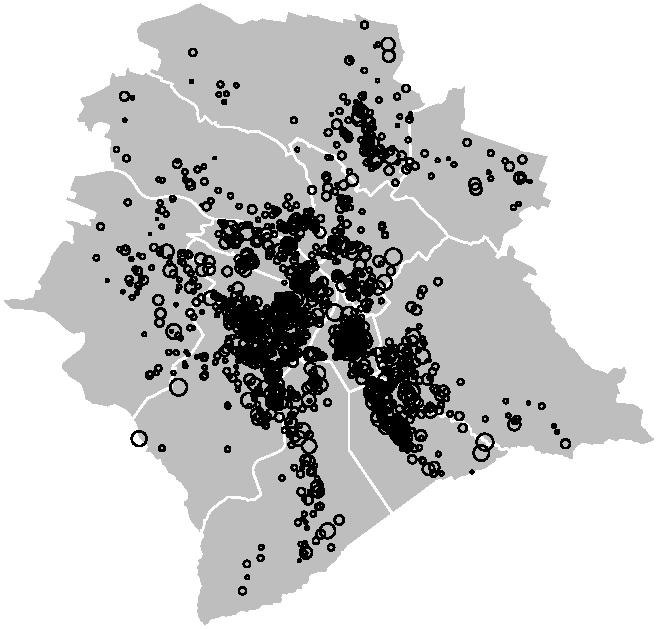
\includegraphics[width=0.95\linewidth]{EcoStat_files/figure-latex/airbnb-1} \caption{Airbnb prices for the Zurich area, 22 June 2017. The size of the circles is proportional to the prices. White lines delineate the 12 districts of the city.}\label{fig:airbnb}
\end{figure}

Let us regress prices on the covariates as well as on district dummies:

\begin{Shaded}
\begin{Highlighting}[]
\NormalTok{eq\_noFE }\OtherTok{\textless{}{-}} \FunctionTok{lm}\NormalTok{(price}\SpecialCharTok{\textasciitilde{}}\NormalTok{bedrooms}\SpecialCharTok{+}\NormalTok{accommodates,}\AttributeTok{data=}\NormalTok{airbnb)}
\NormalTok{eq\_FE   }\OtherTok{\textless{}{-}} \FunctionTok{lm}\NormalTok{(price}\SpecialCharTok{\textasciitilde{}}\NormalTok{bedrooms}\SpecialCharTok{+}\NormalTok{accommodates}\SpecialCharTok{+}\NormalTok{neighborhood,}\AttributeTok{data=}\NormalTok{airbnb)}
\CommentTok{\# Adjust standard errors:}
\NormalTok{cov\_FE          }\OtherTok{\textless{}{-}} \FunctionTok{vcovHC}\NormalTok{(eq\_FE, }\AttributeTok{cluster =}\NormalTok{ airbnb[, }\FunctionTok{c}\NormalTok{(}\StringTok{"neighborhood"}\NormalTok{)])}
\NormalTok{robust\_se\_FE    }\OtherTok{\textless{}{-}} \FunctionTok{sqrt}\NormalTok{(}\FunctionTok{diag}\NormalTok{(cov\_FE))}
\NormalTok{cov\_noFE        }\OtherTok{\textless{}{-}} \FunctionTok{vcovHC}\NormalTok{(eq\_noFE, }\AttributeTok{cluster =}\NormalTok{ airbnb[, }\FunctionTok{c}\NormalTok{(}\StringTok{"neighborhood"}\NormalTok{)])}
\NormalTok{robust\_se\_noFE  }\OtherTok{\textless{}{-}} \FunctionTok{sqrt}\NormalTok{(}\FunctionTok{diag}\NormalTok{(cov\_noFE))}
\NormalTok{stargazer}\SpecialCharTok{::}\FunctionTok{stargazer}\NormalTok{(eq\_FE, eq\_noFE, eq\_FE, eq\_noFE, }\AttributeTok{type =} \StringTok{"text"}\NormalTok{,}
                     \AttributeTok{column.labels =} \FunctionTok{c}\NormalTok{(}\StringTok{"FE (no HAC)"}\NormalTok{, }\StringTok{"No FE (no HAC)"}\NormalTok{,}
                                       \StringTok{"FE (with HAC)"}\NormalTok{, }\StringTok{"No FE (with HAC)"}\NormalTok{),}
                     \AttributeTok{omit =} \FunctionTok{c}\NormalTok{(}\StringTok{"neighborhood"}\NormalTok{),}\AttributeTok{no.space =} \ConstantTok{TRUE}\NormalTok{,}
                     \AttributeTok{omit.labels =} \FunctionTok{c}\NormalTok{(}\StringTok{"District FE"}\NormalTok{),}\AttributeTok{keep.stat =} \StringTok{"n"}\NormalTok{,}
                     \AttributeTok{se =} \FunctionTok{list}\NormalTok{(}\ConstantTok{NULL}\NormalTok{, }\ConstantTok{NULL}\NormalTok{, robust\_se\_FE, robust\_se\_noFE))}
\end{Highlighting}
\end{Shaded}

\begin{verbatim}
## 
## ======================================================================
##                                 Dependent variable:                   
##              ---------------------------------------------------------
##                                        price                          
##              FE (no HAC) No FE (no HAC) FE (with HAC) No FE (with HAC)
##                  (1)          (2)            (3)            (4)       
## ----------------------------------------------------------------------
## bedrooms      7.229***      5.629**       7.229***        5.629***    
##                (2.135)      (2.194)        (2.052)        (2.073)     
## accommodates  16.426***    17.449***      16.426***      17.449***    
##                (1.284)      (1.323)        (1.431)        (1.428)     
## Constant      95.118***    68.417***      95.118***      68.417***    
##                (5.323)      (3.223)        (5.664)        (3.527)     
## ----------------------------------------------------------------------
## District FE      Yes           No            Yes             No       
## ----------------------------------------------------------------------
## Observations    1,321        1,321          1,321          1,321      
## ======================================================================
## Note:                                      *p<0.1; **p<0.05; ***p<0.01
\end{verbatim}

Figure \ref{fig:airbnb3} compares the residuals with and without fixed effects. The sizes of the circles are proportional to the absolute values of the residuals, the color indicates the sign (blue for positive).

\begin{figure}
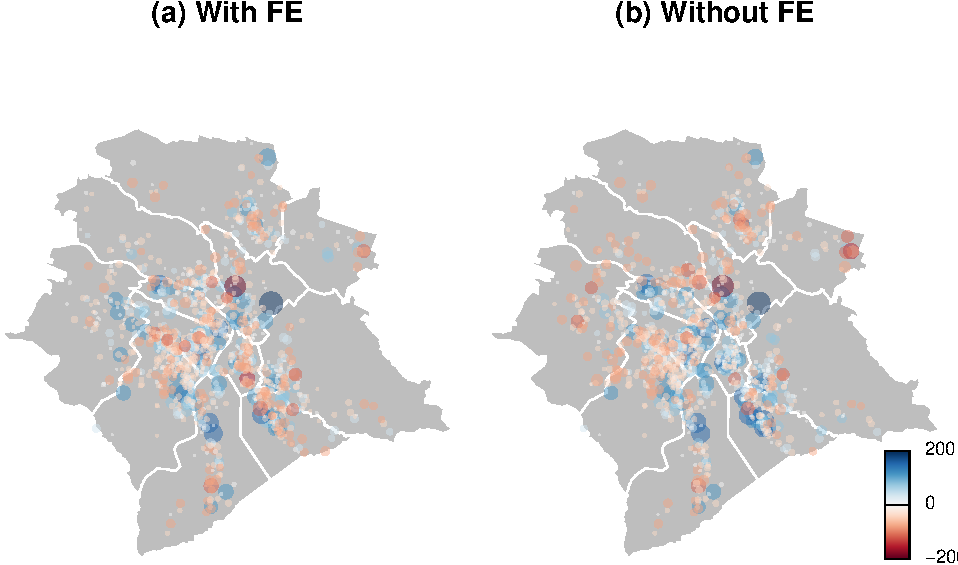
\includegraphics[width=0.95\linewidth]{EcoStat_files/figure-latex/airbnb3-1} \caption{Regression residuals. The sizes of the circles are proportional to the absolute values of the residuals, the color indicates the sign (blue for negative).}\label{fig:airbnb3}
\end{figure}

With fixed effects, the colors are better balanced within each district.
\end{example}

\hypertarget{DynPanel}{%
\section{Dynamic Panel Regressions}\label{DynPanel}}

In what precedes, it has been assumed that there is no correlation between the observations indexed by \((i,t)\) and those indexed by \((j,s)\) as long as \(j \ne i\) or \(t \ne s\). If one suspects that the errors \(\varepsilon_{i,t}\) are correlated (across entities \(i\) for a given date \(t\), or across dates for a given entity, or both), then one should employ a robust covariance matrix (see Section \ref{Clusters}).

In several cases, auto-correlation in the variable of interest may stem from an auto-regressive specification. That is, Eq. \eqref{eq:panel1} is then replaced by:
\begin{equation}
y_{i,t} = \rho y_{i,t-1} + \mathbf{x}'_{i,t}\underbrace{\boldsymbol\beta}_{K \times 1} + \underbrace{\alpha_i}_{\mbox{Individual effects}} + \varepsilon_{i,t}.\label{eq:paneldyn}
\end{equation}

In that case, even if the explanatory variables \(\mathbf{x}_{i,t}\) are uncorrelated to the errors \(\varepsilon_{i,t}\), we have that the additional \emph{explanatory variable} \(y_{i,t-1}\) correlates to the errors \(\varepsilon_{i,t-1},\varepsilon_{i,t-2},\dots,\varepsilon_{i,1}\). As a result, the LSDV estimate of the model parameters \(\{\rho,\boldsymbol\beta\}\) may be biased, even if \(n\) is large. To see this, notice that the LSDV regression amounts to regressing \(\widetilde{\mathbf{y}}\) on \(\widetilde{\mathbf{X}}\) (see Eq. \eqref{eq:bfixedeffects}), where the elements of \(\widetilde{\mathbf{X}}\) are the explanatory variables to which we subtract their within-sample means. In particular, we have:
\[
\tilde{y}_{i,t-1} = y_{i,t-1} - \frac{1}{T} \sum_{s=1}^{T} y_{i,s-1},
\]
which correlates to the corresponding error, that is:
\[
\tilde{\varepsilon}_{i,t} = \varepsilon_{i,t} - \frac{1}{T} \sum_{s=1}^{T} \varepsilon_{i,s}.
\]

The previous equation shows that the \emph{within-group} estimator (LSDV) introduces all realizations of the \(\varepsilon_{i,t}\) errors into the transformed error term (\(\tilde{\varepsilon}_{i,t}\)). As a result, in large-\(n\) fixed-\(T\) panels, it is consistent only if all the right-hand-side variables of the regression are strictly exogenous (i.e., do not correlate to past, present, and future errors \(\varepsilon_{i,t}\)).\footnote{Although the bias may vanish for large \(T\)'s, it does not if \(n\) only goes to infinity.} This is not the case when there are lags of \(y_{i,t}\) on the right-hand side of the regression formula.

The following simulation illustrate this bias. The \(x\)-coordinates of the dots are the fixed effects \(\alpha_i\)'s, and the \(y\)-coordinates are their LSDV estimates. The blue line is the 45-degree line.

\begin{Shaded}
\begin{Highlighting}[]
\NormalTok{n }\OtherTok{\textless{}{-}} \DecValTok{400}\NormalTok{;T }\OtherTok{\textless{}{-}} \DecValTok{10}
\NormalTok{rho }\OtherTok{\textless{}{-}} \FloatTok{0.8}\NormalTok{;sigma }\OtherTok{\textless{}{-}}\NormalTok{ .}\DecValTok{5}
\NormalTok{alpha }\OtherTok{\textless{}{-}} \FunctionTok{rnorm}\NormalTok{(n)}
\NormalTok{y }\OtherTok{\textless{}{-}}\NormalTok{ alpha }\SpecialCharTok{/}\NormalTok{(}\DecValTok{1}\SpecialCharTok{{-}}\NormalTok{rho) }\SpecialCharTok{+}\NormalTok{ sigma}\SpecialCharTok{\^{}}\DecValTok{2}\SpecialCharTok{/}\NormalTok{(}\DecValTok{1} \SpecialCharTok{{-}}\NormalTok{ rho}\SpecialCharTok{\^{}}\DecValTok{2}\NormalTok{) }\SpecialCharTok{*} \FunctionTok{rnorm}\NormalTok{(n)}
\NormalTok{all\_y }\OtherTok{\textless{}{-}}\NormalTok{ y}
\ControlFlowTok{for}\NormalTok{(t }\ControlFlowTok{in} \DecValTok{2}\SpecialCharTok{:}\NormalTok{T)\{}
\NormalTok{  y }\OtherTok{\textless{}{-}}\NormalTok{ rho }\SpecialCharTok{*}\NormalTok{ y }\SpecialCharTok{+}\NormalTok{ alpha }\SpecialCharTok{+}\NormalTok{ sigma }\SpecialCharTok{*} \FunctionTok{rnorm}\NormalTok{(n)}
\NormalTok{  all\_y }\OtherTok{\textless{}{-}} \FunctionTok{rbind}\NormalTok{(all\_y,y)}
\NormalTok{\}}
\NormalTok{y   }\OtherTok{\textless{}{-}} \FunctionTok{c}\NormalTok{(all\_y[}\DecValTok{2}\SpecialCharTok{:}\NormalTok{T,]);y\_1 }\OtherTok{\textless{}{-}} \FunctionTok{c}\NormalTok{(all\_y[}\DecValTok{1}\SpecialCharTok{:}\NormalTok{(T}\DecValTok{{-}1}\NormalTok{),])}
\NormalTok{D }\OtherTok{\textless{}{-}} \FunctionTok{diag}\NormalTok{(n) }\SpecialCharTok{\%x\%} \FunctionTok{rep}\NormalTok{(}\DecValTok{1}\NormalTok{,T}\DecValTok{{-}1}\NormalTok{)}
\NormalTok{Z }\OtherTok{\textless{}{-}} \FunctionTok{cbind}\NormalTok{(}\FunctionTok{c}\NormalTok{(y\_1),D)}
\NormalTok{b }\OtherTok{\textless{}{-}} \FunctionTok{solve}\NormalTok{(}\FunctionTok{t}\NormalTok{(Z) }\SpecialCharTok{\%*\%}\NormalTok{ Z) }\SpecialCharTok{\%*\%} \FunctionTok{t}\NormalTok{(Z) }\SpecialCharTok{\%*\%}\NormalTok{ y}
\NormalTok{a }\OtherTok{\textless{}{-}}\NormalTok{ b[}\DecValTok{2}\SpecialCharTok{:}\NormalTok{(n}\SpecialCharTok{+}\DecValTok{1}\NormalTok{)]}
\FunctionTok{plot}\NormalTok{(alpha,a)}
\FunctionTok{lines}\NormalTok{(}\FunctionTok{c}\NormalTok{(}\SpecialCharTok{{-}}\DecValTok{10}\NormalTok{,}\DecValTok{10}\NormalTok{),}\FunctionTok{c}\NormalTok{(}\SpecialCharTok{{-}}\DecValTok{10}\NormalTok{,}\DecValTok{10}\NormalTok{),}\AttributeTok{col=}\StringTok{"blue"}\NormalTok{)}
\end{Highlighting}
\end{Shaded}

\begin{figure}
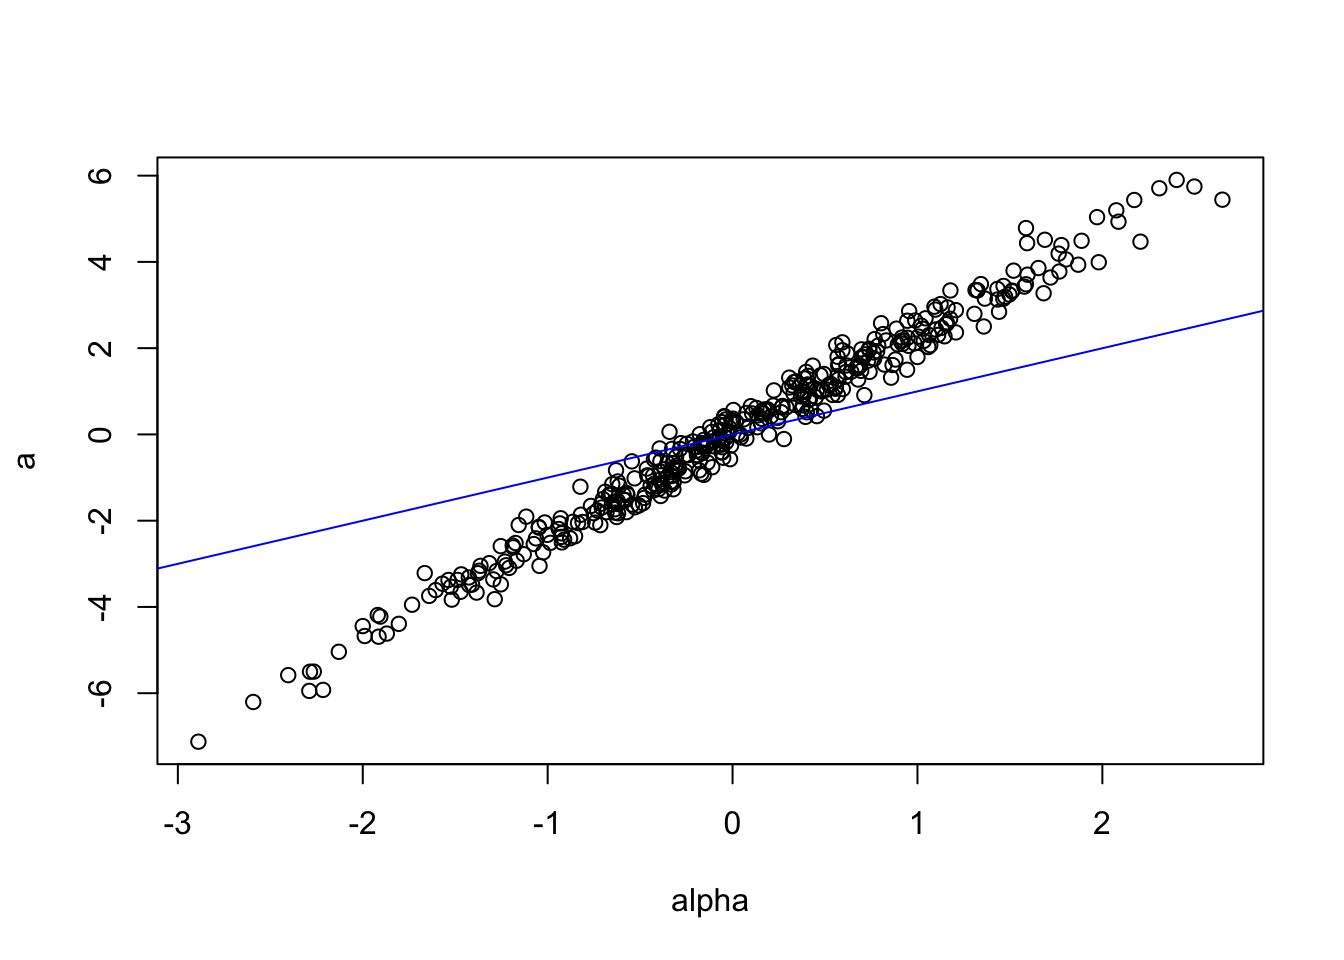
\includegraphics[width=0.95\linewidth]{EcoStat_files/figure-latex/dynpanel1-1} \caption{illustration of the bias pertianing to the LSDV estimation approach in the presence of auto-correlation of the depend variable.}\label{fig:dynpanel1}
\end{figure}

In the previous example, the estimate of \(\rho\) (whose true value is 0.8) is 0.531.

To address this, one can resort to instrumental-variable regressions. \citet{Anderson_Hsiao_1982} have, in particular, proposed a first-differenced Two Stage Least Squares (2SLS) estimator (see Eq. \eqref{eq:IV} in Section \ref{IV}). This estimation is based on the following transformation of the model:
\begin{equation}
\Delta y_{i,t} = \rho \Delta y_{i,t-1} + (\Delta \mathbf{x}_{i,t})'\boldsymbol\beta + \Delta\varepsilon_{i,t}.\label{eq:paneldynFisrtDiff}
\end{equation}
The OLS estimates of the parameters are biased because \(\varepsilon_{i,t-1}\) ---which is part of the error \(\Delta\varepsilon_{i,t}\)--- is correlated to \(y_{i,t-1}\) ---which is part of the ``explanatory variable'', namely \(\Delta y_{i,t-1}\). But consistent estimates can be obtained using 2SLS with instrumental variables that are correlated with \(\Delta y_{i,t}\) but orthogonal to \(\Delta\varepsilon_{i,t}\). One can for instance use \(\{y_{i,t-2},\mathbf{x}_{i,t-2}\}\) as instruments. Note that this approach can be implemented only if there are more than 3 time observations per entity \(i\).

If the explanatory variables \(\mathbf{x}_{i,t}\) are assumed to be predetermined (i.e., do not contemporaneous correlate with the errors \(\varepsilon_{i,t}\)), then \(\mathbf{x}_{i,t-1}\) can be added to the instruments associated with \(\Delta y_{i,t}\). Further, if these variables (the \(\mathbf{x}_{i,t}\)'s) are exogenous (i.e., do not contemporaneous correlate with any of the errors \(\varepsilon_{i,s}\), \(\forall s\)), then \(\mathbf{x}_{i,t}\) also constitute a valid instrument.

Using the previous (simulated) example, this approach consists in the following steps:

\begin{Shaded}
\begin{Highlighting}[]
\NormalTok{Dy   }\OtherTok{\textless{}{-}} \FunctionTok{c}\NormalTok{(all\_y[}\DecValTok{3}\SpecialCharTok{:}\NormalTok{T,]) }\SpecialCharTok{{-}} \FunctionTok{c}\NormalTok{(all\_y[}\DecValTok{2}\SpecialCharTok{:}\NormalTok{(T}\DecValTok{{-}1}\NormalTok{),])}
\NormalTok{Dy\_1 }\OtherTok{\textless{}{-}} \FunctionTok{c}\NormalTok{(all\_y[}\DecValTok{2}\SpecialCharTok{:}\NormalTok{(T}\DecValTok{{-}1}\NormalTok{),]) }\SpecialCharTok{{-}} \FunctionTok{c}\NormalTok{(all\_y[}\DecValTok{1}\SpecialCharTok{:}\NormalTok{(T}\DecValTok{{-}2}\NormalTok{),])}
\NormalTok{y\_2  }\OtherTok{\textless{}{-}} \FunctionTok{c}\NormalTok{(all\_y[}\DecValTok{1}\SpecialCharTok{:}\NormalTok{(T}\DecValTok{{-}2}\NormalTok{),])}
\NormalTok{Z }\OtherTok{\textless{}{-}} \FunctionTok{matrix}\NormalTok{(y\_2,}\AttributeTok{ncol=}\DecValTok{1}\NormalTok{)}
\NormalTok{Pz }\OtherTok{\textless{}{-}}\NormalTok{ Z }\SpecialCharTok{\%*\%} \FunctionTok{solve}\NormalTok{(}\FunctionTok{t}\NormalTok{(Z) }\SpecialCharTok{\%*\%}\NormalTok{ Z) }\SpecialCharTok{\%*\%} \FunctionTok{t}\NormalTok{(Z)}
\NormalTok{Dy\_1hat }\OtherTok{\textless{}{-}}\NormalTok{ Pz }\SpecialCharTok{\%*\%}\NormalTok{ Dy\_1}
\NormalTok{rho\_2SLS }\OtherTok{\textless{}{-}} \FunctionTok{solve}\NormalTok{(}\FunctionTok{t}\NormalTok{(Dy\_1hat) }\SpecialCharTok{\%*\%}\NormalTok{ Dy\_1hat) }\SpecialCharTok{\%*\%} \FunctionTok{t}\NormalTok{(Dy\_1hat) }\SpecialCharTok{\%*\%}\NormalTok{ Dy}
\end{Highlighting}
\end{Shaded}

While the OLS estimate of \(\rho\) (whose true value is 0.8) was 0.531, we obtain here \texttt{rho\_2SLS} \(=\) 0.89.

Let us come back to the general case (with covariates \(\mathbf{x}_{i,k}\)'s). For \(t=3\), \(y_{i,1}\) (and \(\mathbf{x}_{i,1}\)) is the only possible instrument. However, for \(t=4\), one could use \(y_{i,2}\) and \(y_{i,1}\) (as well as \(\mathbf{x}_{i,2}\) and \(\mathbf{x}_{i,1}\)). More generally, defining matrix \(Z_i\) as follows:
\[
Z_i = \left[
\begin{array}{ccccccccccccccccc}
\mathbf{z}_{i,1}' & 0 & \dots \\
0 & \mathbf{z}_{i,1}' & \mathbf{z}_{i,2}' & 0 & \dots \\
0 &0 &0 & \mathbf{z}_{i,1} & \mathbf{z}_{i,2}' & \mathbf{z}_{i,3}' & 0 & \dots \\
\vdots \\
0 & \dots &&&&&& 0 & \mathbf{z}_{i,1}' &  \dots &   \mathbf{z}_{i,T-2}'
\end{array}
\right],
\]
where \(\mathbf{z}_{i,t} = [y_{i,t},\mathbf{x}_{i,t}']'\), we have the moment conditions:\footnote{If \(\mathbf{x}_{i,t}\) is predetermined (exogenous), we can use \(\mathbf{z}_{i,t} = [y_{i,t},\mathbf{x}_{i,t+1},\mathbf{x}_{i,t}']'\) (respectively \(\mathbf{z}_{i,t} = [y_{i,t},\mathbf{x}_{i,t+2},\mathbf{x}_{i,t+1},\mathbf{x}_{i,t}']'\)).}
\[
\mathbb{E}(Z_i'\Delta  {\boldsymbol\varepsilon}_i)=0,
\]

with \(\Delta{\boldsymbol\varepsilon}_i = [ \Delta \varepsilon_{i,3},\dots,\Delta \varepsilon_{i,T}]'\).

These restrictions are used in the GMM approach employed by \citet{Arellano_Bond_1991}. Specifically, a GMM estimator of the model parameters is given by:
\[
\mbox{argmin}\;\left(\frac{1}{n} \sum_{i=1}^n Z_i' \Delta \boldsymbol\varepsilon_i\right)'W_n\left(\frac{1}{n} \sum_{i=1}^n Z_i' \Delta \boldsymbol\varepsilon_i\right),
\]
using the weighting matrix
\[
W_n = \left(\frac{1}{n}\sum_{i=1}^n Z_i'\widehat{\Delta\boldsymbol\varepsilon_i}\widehat{\Delta\boldsymbol\varepsilon_i}'Z_i\right)^{-1},
\]
where the \(\widehat{\Delta\boldsymbol\varepsilon_i}\)'s are consistent estimates of the \(\Delta\boldsymbol\varepsilon_i\)'s that result from a preliminary estimation. In this sense, this estimator is a two-step GMM one.

If the disturbances are homoskedastic, then it can be shown that an asymptotically equivalent (efficient) GMM estimator can be obtained by using:
\[
W_{1,n} = \left(\frac{1}{n}Z_i'HZ_i\right)^{-1},
\]
where \(H\) is is \((T-2) \times (T-2)\) matrix of the form:
\[
H = \left[\begin{array}{ccccccc}
2 & -1 & 0 & \dots &0 \\
-1 & 2 & -1 &  & \vdots \\
0 & \ddots& \ddots & \ddots & 0 \\
\vdots &  & -1 & 2&-1\\
0&\dots & 0 & -1 & 2
\end{array}\right].
\]

It is straightforward to extend these GMM methods to cases where there is more than one lag of the dependent variable on the right-hand side of the equation or in cases where disturbances feature limited moving-average serial correlation.

The \texttt{pdynmc} package allows to run these GMM approaches (see \citet{Fritsch_et_al_2019}). The following lines of code allow to replicate the results of \citet{Arellano_Bond_1991}:

\begin{Shaded}
\begin{Highlighting}[]
\FunctionTok{library}\NormalTok{(pdynmc)}
\FunctionTok{data}\NormalTok{(EmplUK, }\AttributeTok{package =} \StringTok{"plm"}\NormalTok{)}
\NormalTok{dat }\OtherTok{\textless{}{-}}\NormalTok{ EmplUK}
\NormalTok{dat[,}\FunctionTok{c}\NormalTok{(}\DecValTok{4}\SpecialCharTok{:}\DecValTok{7}\NormalTok{)]         }\OtherTok{\textless{}{-}} \FunctionTok{log}\NormalTok{(dat[,}\FunctionTok{c}\NormalTok{(}\DecValTok{4}\SpecialCharTok{:}\DecValTok{7}\NormalTok{)])}
\NormalTok{m1 }\OtherTok{\textless{}{-}} \FunctionTok{pdynmc}\NormalTok{(}\AttributeTok{dat =}\NormalTok{ dat, }\CommentTok{\# name of the dataset}
             \AttributeTok{varname.i =} \StringTok{"firm"}\NormalTok{, }\CommentTok{\# name of the cross{-}section identifier}
             \AttributeTok{varname.t =} \StringTok{"year"}\NormalTok{, }\CommentTok{\# name of the time{-}series identifiers}
             \AttributeTok{use.mc.diff =} \ConstantTok{TRUE}\NormalTok{, }\CommentTok{\# use moment conditions from equations in differences? (i.e. instruments in levels) }
             \AttributeTok{use.mc.lev =} \ConstantTok{FALSE}\NormalTok{, }\CommentTok{\# use moment conditions from equations in levels? (i.e. instruments in differences)}
             \AttributeTok{use.mc.nonlin =} \ConstantTok{FALSE}\NormalTok{, }\CommentTok{\# use nonlinear (quadratic) moment conditions?}
             \AttributeTok{include.y =} \ConstantTok{TRUE}\NormalTok{, }\CommentTok{\# instruments should be derived from the lags of the dependent variable?}
             \AttributeTok{varname.y =} \StringTok{"emp"}\NormalTok{, }\CommentTok{\# name of the dependent variable in the dataset}
             \AttributeTok{lagTerms.y =} \DecValTok{2}\NormalTok{, }\CommentTok{\# number of lags of the dependent variable}
             \AttributeTok{fur.con =} \ConstantTok{TRUE}\NormalTok{, }\CommentTok{\# further control variables (covariates) are included?}
             \AttributeTok{fur.con.diff =} \ConstantTok{TRUE}\NormalTok{, }\CommentTok{\# include further control variables in equations from differences ?}
             \AttributeTok{fur.con.lev =} \ConstantTok{FALSE}\NormalTok{, }\CommentTok{\# include further control variables in equations from level?}
             \AttributeTok{varname.reg.fur =} \FunctionTok{c}\NormalTok{(}\StringTok{"wage"}\NormalTok{, }\StringTok{"capital"}\NormalTok{, }\StringTok{"output"}\NormalTok{), }\CommentTok{\# covariate(s) {-}in the dataset{-} to treat as further controls}
             \AttributeTok{lagTerms.reg.fur =} \FunctionTok{c}\NormalTok{(}\DecValTok{1}\NormalTok{,}\DecValTok{2}\NormalTok{,}\DecValTok{2}\NormalTok{), }\CommentTok{\# number of lags of the further controls}
             \AttributeTok{include.dum =} \ConstantTok{TRUE}\NormalTok{, }\CommentTok{\# A logical variable indicating whether dummy variables for the time periods are included (defaults to \textquotesingle{}FALSE\textquotesingle{}).}
             \AttributeTok{dum.diff =} \ConstantTok{TRUE}\NormalTok{, }\CommentTok{\# A logical variable indicating whether dummy variables are included in the equations in first differences (defaults to \textquotesingle{}NULL\textquotesingle{}).}
             \AttributeTok{dum.lev =} \ConstantTok{FALSE}\NormalTok{, }\CommentTok{\# A logical variable indicating whether dummy variables are included in the equations in levels (defaults to \textquotesingle{}NULL\textquotesingle{}).}
             \AttributeTok{varname.dum =} \StringTok{"year"}\NormalTok{,}
             \AttributeTok{w.mat =} \StringTok{"iid.err"}\NormalTok{, }\CommentTok{\# One of the character strings c(\textquotesingle{}"iid.err"\textquotesingle{}, \textquotesingle{}"identity"\textquotesingle{}, \textquotesingle{}"zero.cov"\textquotesingle{}) indicating the type of weighting matrix to use (defaults to \textquotesingle{}"iid.err"\textquotesingle{})}
             \AttributeTok{std.err =} \StringTok{"corrected"}\NormalTok{,}
             \AttributeTok{estimation =} \StringTok{"onestep"}\NormalTok{, }\CommentTok{\# One of the character strings c(\textquotesingle{}"onestep"\textquotesingle{}, \textquotesingle{}"twostep"\textquotesingle{}, \textquotesingle{}"iterative"\textquotesingle{}). Denotes the number of iterations of the parameter procedure (defaults to \textquotesingle{}"twostep"\textquotesingle{}).}
             \AttributeTok{opt.meth =} \StringTok{"none"} \CommentTok{\# numerical optimization procedure. When no nonlinear moment conditions are employed in estimation, closed form estimates can be computed by setting the argument to \textquotesingle{}"none"}
\NormalTok{)}
\FunctionTok{summary}\NormalTok{(m1,}\AttributeTok{digits=}\DecValTok{3}\NormalTok{)}
\end{Highlighting}
\end{Shaded}

\begin{verbatim}
## 
## Dynamic linear panel estimation (onestep)
## Estimation steps: 1
## 
## Coefficients:
##             Estimate Std.Err.rob z-value.rob Pr(>|z.rob|)    
## L1.emp      0.686226    0.144594       4.746      < 2e-16 ***
## L2.emp     -0.085358    0.056016      -1.524      0.12751    
## L0.wage    -0.607821    0.178205      -3.411      0.00065 ***
## L1.wage     0.392623    0.167993       2.337      0.01944 *  
## L0.capital  0.356846    0.059020       6.046      < 2e-16 ***
## L1.capital -0.058001    0.073180      -0.793      0.42778    
## L2.capital -0.019948    0.032713      -0.610      0.54186    
## L0.output   0.608506    0.172531       3.527      0.00042 ***
## L1.output  -0.711164    0.231716      -3.069      0.00215 ** 
## L2.output   0.105798    0.141202       0.749      0.45386    
## 1979        0.009554    0.010290       0.929      0.35289    
## 1980        0.022015    0.017710       1.243      0.21387    
## 1981       -0.011775    0.029508      -0.399      0.68989    
## 1982       -0.027059    0.029275      -0.924      0.35549    
## 1983       -0.021321    0.030460      -0.700      0.48393    
## 1976       -0.007703    0.031411      -0.245      0.80646    
## ---
## Signif. codes:  0 '***' 0.001 '**' 0.01 '*' 0.05 '.' 0.1 ' ' 1
## 
##  41 total instruments are employed to estimate 16 parameters
##  27 linear (DIF) 
##  8 further controls (DIF) 
##  6 time dummies (DIF) 
##  
## J-Test (overid restrictions):  70.82 with 25 DF, pvalue: <0.001
## F-Statistic (slope coeff):  528.06 with 10 DF, pvalue: <0.001
## F-Statistic (time dummies):  14.98 with 6 DF, pvalue: 0.0204
\end{verbatim}

We generate novel results (\texttt{m2}) by replacing ``\texttt{onestep}'' with ``\texttt{twostep}'' (in the \texttt{estimation} field). The resulting estimated coefficients are:

\begin{verbatim}
##      L1.emp      L2.emp     L0.wage     L1.wage  L0.capital  L1.capital 
##  0.62870890 -0.06518800 -0.52575951  0.31128961  0.27836190  0.01409950 
##  L2.capital   L0.output   L1.output   L2.output        1979        1980 
## -0.04024847  0.59192286 -0.56598515  0.10054264  0.01121551  0.02306871 
##        1981        1982        1983        1976 
## -0.02135806 -0.03111604 -0.01799335 -0.02336762
\end{verbatim}

\citet{Arellano_Bond_1991} have proposed a specification test. If the model is correctly specified, then the errors of Eq. \eqref{eq:paneldynFisrtDiff} ---that is the first-difference equation--- should feature non-zero first-order auto-correlations, but zero higher-order autocorrelations.

Function \texttt{mtest.fct} of package \texttt{pdynmc} implements this test. Here is its result in the present case:

\begin{Shaded}
\begin{Highlighting}[]
\FunctionTok{mtest.fct}\NormalTok{(m1,}\AttributeTok{order=}\DecValTok{3}\NormalTok{)}
\end{Highlighting}
\end{Shaded}

\begin{verbatim}
## 
##  Arellano and Bond (1991) serial correlation test of degree 3
## 
## data:  1step GMM Estimation
## normal = 0.045945, p-value = 0.9634
## alternative hypothesis: serial correlation of order 3 in the error terms
\end{verbatim}

One can also implement the Hansen J-test of the over-identifying restrictions (see Section \ref{overidentif}):

\begin{Shaded}
\begin{Highlighting}[]
\FunctionTok{jtest.fct}\NormalTok{(m1)}
\end{Highlighting}
\end{Shaded}

\begin{verbatim}
## 
##  J-Test of Hansen
## 
## data:  1step GMM Estimation
## chisq = 70.82, df = 25, p-value = 2.905e-06
## alternative hypothesis: overidentifying restrictions invalid
\end{verbatim}

\begin{Shaded}
\begin{Highlighting}[]
\FunctionTok{jtest.fct}\NormalTok{(m2)}
\end{Highlighting}
\end{Shaded}

\begin{verbatim}
## 
##  J-Test of Hansen
## 
## data:  2step GMM Estimation
## chisq = 31.381, df = 25, p-value = 0.1767
## alternative hypothesis: overidentifying restrictions invalid
\end{verbatim}

\hypertarget{introduction-to-program-evaluation}{%
\section{Introduction to program evaluation}\label{introduction-to-program-evaluation}}

This section brielfy introduces the econometrics of program evaluation. Program evaluation refer to the analysis of the causal effects of some ``treatments'' in a broad sense. These treatment can, e.g., correspond to the implementation (or announcement) of policy measures. A comprehensive review is proposed by \citet{Abadie_Cattaneo_2018}. A seminal book on the subject is that of \citet{angrist_mostly_2008}.

\hypertarget{presentation-of-the-problem}{%
\subsection{Presentation of the problem}\label{presentation-of-the-problem}}

To begin with, let us consider a single entity. To simplify notations, we drop the entity index (\(i\)). Let us denote by \(Y\) the outcome variable (for the variable of interest), by \(W\) is a binary variable indicating whether the considered entity has received treatment (\(W=1\)) or not (\(W=0\)), and by \(X\) a vector of covariates, assumed to be predetermined relative to the treatment. That is, \(W\) and \(X\) could be correlated, but the values of \(X\) have been determined before that of \(W\) (in such a way that the realization of \(W\) does not affect \(X\)). Typcally, \(X\) contains characteristics of the considered entity.

We are interested in the effect of the treatment, that is:
\[
Y_1 - Y_0,
\]
where \(Y_1\) correspond to the outcome obtained under treatment, while \(Y_0\) is the outcome obtained without it. Notice that we have:
\[
Y = (1-W) Y_0 + W Y_1.
\]

The problem is that observing \((Y,W,X)\) is not sufficient to observe the treatment effect \(Y_1 - Y_0\). Additional assumptions are needed to estimate it, or, more precisely, its expectations (\emph{average treatment effect}):
\[
ATE = \mathbb{E}(Y_1 - Y_0).
\]

Importantly, \(ATE\) is different from the following quantity:
\[
\alpha = \underbrace{\mathbb{E}(Y|W=1)}_{=\mathbb{E}(Y_1|W=1)} - \underbrace{\mathbb{E}(Y|W=0)}_{=\mathbb{E}(Y_0|W=0)},
\]
that is easier to estimate. Indeed, a consistent estimate of \(\alpha\) is the difference between the means of the outcome variables in two sub-samples: one containing only the treated entities (this gives an estimate of \(\mathbb{E}(Y_1|W=1)\)) and the other containing only the non-treated entities (this gives an estimate of \(\mathbb{E}(Y_0|W=0)\)). Coming back to \(ATE\), the problem is that we won't have direct information regarding \(\mathbb{E}(Y_0|W=1)\) and \(\mathbb{E}(Y_1|W=0)\). However, these two conditional expectations are part of \(ATE\). Indeed, \(ATE = \mathbb{E}(Y_1) - \mathbb{E}(Y_0)\), and:
\begin{eqnarray}
\mathbb{E}(Y_1) &=& \mathbb{E}(Y_1|W=0)\mathbb{P}(W=0)+\mathbb{E}(Y_1|W=1)\mathbb{P}(W=1) \label{eq:EY1a} \\
\mathbb{E}(Y_0) &=& \mathbb{E}(Y_0|W=0)\mathbb{P}(W=0)+\mathbb{E}(Y_0|W=1)\mathbb{P}(W=1). \label{eq:EY0a}
\end{eqnarray}

\hypertarget{randomized-controlled-trials-rcts}{%
\subsection{Randomized controlled trials (RCTs)}\label{randomized-controlled-trials-rcts}}

In the context of Randomized controlled trials (RCTs), entities are randomly assigned to receive the treatment. As a result, we have \(\mathbb{E}(Y_1) = \mathbb{E}(Y_1|W=0) = \mathbb{E}(Y_1|W=1)\) and \(\mathbb{E}(Y_0) = \mathbb{E}(Y_0|W=0) = \mathbb{E}(Y_0|W=1)\). Using this into Eqs. \eqref{eq:EY1a} and \eqref{eq:EY0a} yields \(ATE = \alpha\).

Therefore, in this context, estimating \(\mathbb{E}(Y_1-Y_0)\) amounts to computing the difference between two sample means, namely (a) the sample mean of the subset of \(Y_i\)'s corresponding to the entities for which \(W_i=1\), and (b) the one for which \(W_i=0\).

More accurate estimates can be obtained through regressions. Assume that the model reads:
\[
Y_{i} = W_{i} \beta_{1} + X_i'\boldsymbol\beta_z + \varepsilon_i,
\]
where \(\mathbb{E}(\varepsilon_i|X_i) = 0\) (and \(W_i\) is independent from \(X_i\) and \(\varepsilon_i\)). In this case, we obtain a consistent estimate of \(\beta_1\) by regressing \(\mathbf{y}\) on \(\mathbf{Z} = [\mathbf{w},\mathbf{X}]\).

\hypertarget{difference-in-difference-did-approach}{%
\subsection{Difference-in-Difference (DiD) approach}\label{difference-in-difference-did-approach}}

The DiD approach is a popular methodology implemented in cases where \(W\) cannot be considered as an independent variable. It exploits two dimensions: entities (\(i\)), and time (\(t\)). To simplify the exposition, we consider only two periods here (\(t=0\) and \(t=1\)).

Consider the following model:
\begin{equation}
Y_{i,t} = W_{i,t} \beta_1 + \mu_i + \delta_t + \varepsilon_{i,t}\label{eq:DiD}
\end{equation}

The parameter of interest is \(\beta_{1}\), which is the treatment effect (recall that \(W_{i,t} \in \{0,1\}\)). Usually, for all entities \(i\), we have \(W_{i,t=0}=0\). But only some of them are treated on date 1, i.e., \(W_{i,1} \in \{0,1\}\).

The disturbance \(\varepsilon_{i,t}\) affects the outcome, but we assume that it does not relate to the selection for treatment; therefore, \(\mathbb{E}(\varepsilon_{i,t}|W_{i,t})=0\). By contrast, we do not exclude some correlation between \(W_{i,t}\) (for \(t=1\)) and \(\mu_i\); hence, \(\mu_i\) may constitute a \emph{confounder}. Finally, we suppose that the micro-variables \(W_i\) do not affect the time fixed effects \(\delta_t\), such that \(\mathbb{E}(\delta_t|W_{i,t})=\mathbb{E}(\delta_t)\).

We have:

\[
\begin{array}{cccccccccc}
\mathbb{E}(Y_{i,1}|W_{i,1}=1) &=& \beta_1 &+& \mathbb{E}(\mu_i|W_{i,1}=1) &+&\mathbb{E}(\delta_1|W_{i,1}=1) &+& \mathbb{E}(\varepsilon_{i,1}) \\
\mathbb{E}(Y_{i,0}|W_{i,1}=1) &=&  && \mathbb{E}(\mu_i|W_{i,1}=1) &+&\mathbb{E}(\delta_0|W_{i,1}=1) &+& \mathbb{E}(\varepsilon_{i,0}) \\
\mathbb{E}(Y_{i,1}|W_{i,1}=0) &=& && \mathbb{E}(\mu_i|W_{i,1}=0) &+&\mathbb{E}(\delta_1|W_{i,1}=0) &+& \mathbb{E}(\varepsilon_{i,1}) \\
\mathbb{E}(Y_{i,0}|W_{i,1}=0) &=&  && \mathbb{E}(\mu_i|W_{i,1}=0) &+&\mathbb{E}(\delta_0|W_{i,1}=0) &+& \mathbb{E}(\varepsilon_{i,0}).
\end{array}
\]
and, under our assumptions, it can be checked that:

\[
\beta_1 = \mathbb{E}(\Delta Y_{i,1}|W_{i,1}=1) - \mathbb{E}(\Delta Y_{i,1}|W_{i,1}=0),
\]
where \(\Delta Y_{i,1}=Y_{i,1}-Y_{i,0}\). Therefore, in this context, the treatment effect appears to be a difference (of two conditionnal expectations) of difference (of the outcome variable, through time).

This is illustrated by Figure \ref{fig:figAbadie}, which represents the generic DiD framework.

\begin{figure}

{\centering 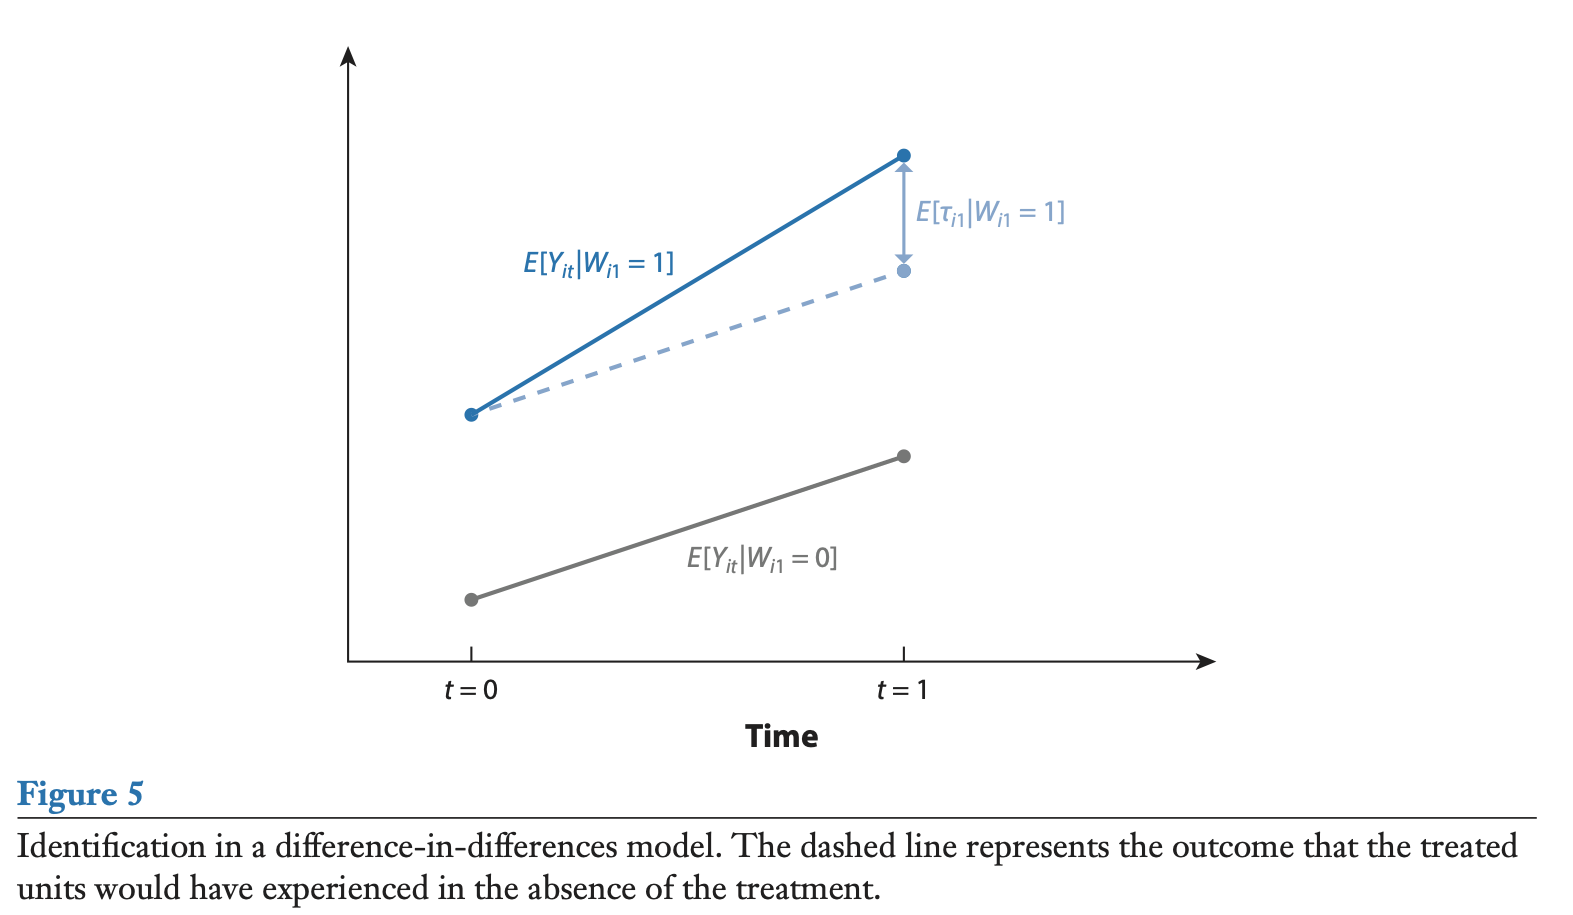
\includegraphics[width=0.95\linewidth]{images/Abadie_et_al_2018} 

}

\caption{Source: Abadie et al., (1998).}\label{fig:figAbadie}
\end{figure}

In practice, implementing this approach consists in running a linear regression of the type of Eq. \eqref{eq:DiD}. These regressions also usually involve controls on top of the fixed effects \(\mu_i\). As illustrated in the next subsection, the parameter of interest (\(\beta_1\)) is often associated with an interaction term.

\hypertarget{application-of-the-did-approach}{%
\subsection{Application of the DiD approach}\label{application-of-the-did-approach}}

This example is based on the data used in \citet{Meyer_Viscusi_Durbin_1995}. This dataset is part of the \texttt{wooldridge} package. This paper examines the effect of workers' compensation for injury on time out of work. It exploits a \textbf{natural experiment} approach of comparing individuals injured before and after increases in the maximum weekly benefit amount. Specifically, in 1980, the cap on weekly earnings covered by worker's compensation was increased in Kentucky and Michigan. Let us check whether this new policy was followed by an increase in the amount of time workers spent unemployed (for example, higher compensation may reduce workers' incentives to avoid injury).

As shown in Figure \ref{fig:figMeyer}, the measure has only affected high-earning workers. The idea exploited by \citet{Meyer_Viscusi_Durbin_1995} was to compare the increase in time out of work before-after 1980 for higher-earnings workers on the one hand (entities who received the treatment) and low-earnings workers on the other hand (control group).

\begin{figure}

{\centering 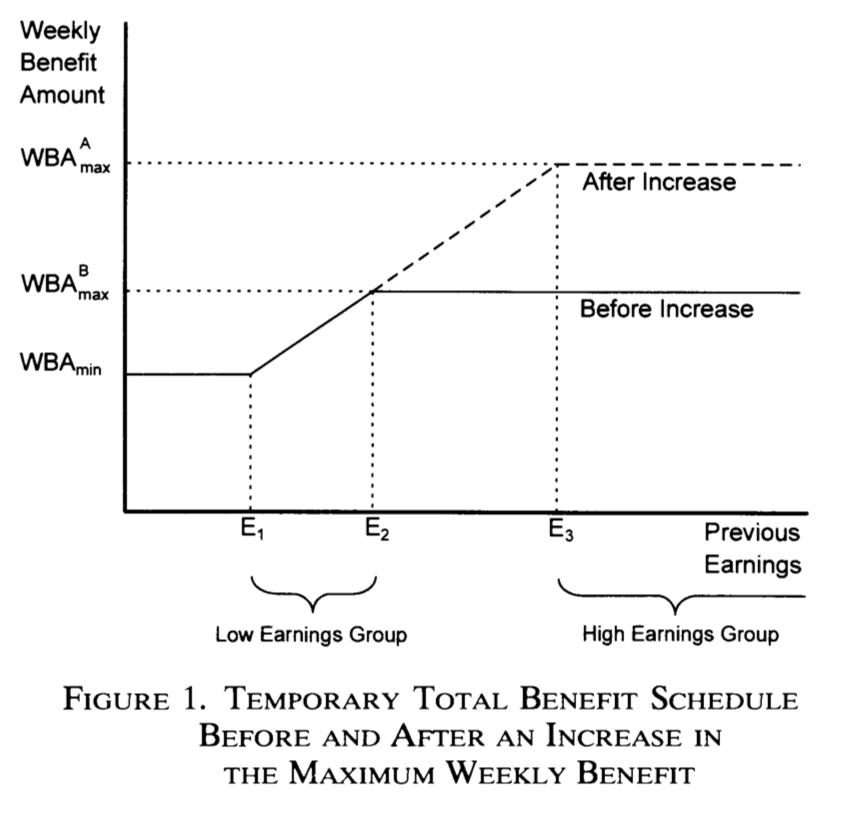
\includegraphics[width=0.9\linewidth]{images/Figure_Meyer_et_al} 

}

\caption{Source: Meyer et al., (1995).}\label{fig:figMeyer}
\end{figure}

The next lines of codes replicate some of their results. The dependent variable is the logarithm of the duration of benefits. For more information use \texttt{?injury}, after having loaded the \texttt{wooldridge} library.

In the table of results below, the parameter of interest is the one associated with the interaction term \texttt{afchnge:highearn}. Columns 2 and 3 correspond to the first two column of Table 6 in \citet{Meyer_Viscusi_Durbin_1995}.

\begin{Shaded}
\begin{Highlighting}[]
\FunctionTok{library}\NormalTok{(wooldridge)}
\FunctionTok{data}\NormalTok{(injury)}
\NormalTok{injury }\OtherTok{\textless{}{-}} \FunctionTok{subset}\NormalTok{(injury,ky}\SpecialCharTok{==}\DecValTok{1}\NormalTok{)}
\NormalTok{injury}\SpecialCharTok{$}\NormalTok{indust }\OtherTok{\textless{}{-}} \FunctionTok{as.factor}\NormalTok{(injury}\SpecialCharTok{$}\NormalTok{indust)}
\NormalTok{injury}\SpecialCharTok{$}\NormalTok{injtype }\OtherTok{\textless{}{-}} \FunctionTok{as.factor}\NormalTok{(injury}\SpecialCharTok{$}\NormalTok{injtype)}
\CommentTok{\#names(injury)}
\NormalTok{eq1 }\OtherTok{\textless{}{-}} \FunctionTok{lm}\NormalTok{(}\FunctionTok{log}\NormalTok{(durat) }\SpecialCharTok{\textasciitilde{}}\NormalTok{ afchnge }\SpecialCharTok{+}\NormalTok{ highearn }\SpecialCharTok{+}\NormalTok{ afchnge}\SpecialCharTok{*}\NormalTok{highearn,}\AttributeTok{data=}\NormalTok{injury)}
\NormalTok{eq2 }\OtherTok{\textless{}{-}} \FunctionTok{lm}\NormalTok{(}\FunctionTok{log}\NormalTok{(durat) }\SpecialCharTok{\textasciitilde{}}\NormalTok{ afchnge }\SpecialCharTok{+}\NormalTok{ highearn }\SpecialCharTok{+}\NormalTok{ afchnge}\SpecialCharTok{*}\NormalTok{highearn }\SpecialCharTok{+}
\NormalTok{            lprewage}\SpecialCharTok{*}\NormalTok{highearn }\SpecialCharTok{+}\NormalTok{ male }\SpecialCharTok{+}\NormalTok{ married }\SpecialCharTok{+}\NormalTok{ lage }\SpecialCharTok{+}\NormalTok{ ltotmed }\SpecialCharTok{+}\NormalTok{ hosp }\SpecialCharTok{+}
\NormalTok{            indust }\SpecialCharTok{+}\NormalTok{ injtype,}\AttributeTok{data=}\NormalTok{injury)}
\NormalTok{eq3 }\OtherTok{\textless{}{-}} \FunctionTok{lm}\NormalTok{(}\FunctionTok{log}\NormalTok{(durat) }\SpecialCharTok{\textasciitilde{}}\NormalTok{ afchnge }\SpecialCharTok{+}\NormalTok{ highearn }\SpecialCharTok{+}\NormalTok{ afchnge}\SpecialCharTok{*}\NormalTok{highearn }\SpecialCharTok{+}
\NormalTok{            lprewage}\SpecialCharTok{*}\NormalTok{highearn }\SpecialCharTok{+}\NormalTok{ male }\SpecialCharTok{+}\NormalTok{ married }\SpecialCharTok{+}\NormalTok{ lage }\SpecialCharTok{+}\NormalTok{ indust }\SpecialCharTok{+}
\NormalTok{            injtype,}\AttributeTok{data=}\NormalTok{injury)}
\NormalTok{stargazer}\SpecialCharTok{::}\FunctionTok{stargazer}\NormalTok{(eq1,eq2,eq3,}\AttributeTok{type=}\StringTok{"text"}\NormalTok{,}
                     \AttributeTok{omit=}\FunctionTok{c}\NormalTok{(}\StringTok{"indust"}\NormalTok{,}\StringTok{"injtype"}\NormalTok{,}\StringTok{"Constant"}\NormalTok{),}\AttributeTok{no.space =} \ConstantTok{TRUE}\NormalTok{,}
                     \AttributeTok{add.lines =} \FunctionTok{list}\NormalTok{(}\FunctionTok{c}\NormalTok{(}\StringTok{"industry dummy"}\NormalTok{,}\StringTok{"no"}\NormalTok{,}\StringTok{"yes"}\NormalTok{,}\StringTok{"yes"}\NormalTok{),}
                                      \FunctionTok{c}\NormalTok{(}\StringTok{"injury dummy"}\NormalTok{,}\StringTok{"no"}\NormalTok{,}\StringTok{"yes"}\NormalTok{,}\StringTok{"yes"}\NormalTok{)),}
                     \AttributeTok{order =} \FunctionTok{c}\NormalTok{(}\DecValTok{1}\NormalTok{,}\DecValTok{2}\NormalTok{,}\DecValTok{18}\NormalTok{,}\DecValTok{3}\SpecialCharTok{:}\DecValTok{17}\NormalTok{,}\DecValTok{19}\NormalTok{,}\DecValTok{20}\NormalTok{),}\AttributeTok{omit.stat =} \FunctionTok{c}\NormalTok{(}\StringTok{"f"}\NormalTok{,}\StringTok{"ser"}\NormalTok{))}
\end{Highlighting}
\end{Shaded}

\begin{verbatim}
## 
## ===============================================
##                        Dependent variable:     
##                   -----------------------------
##                            log(durat)          
##                      (1)       (2)       (3)   
## -----------------------------------------------
## afchnge             0.008    -0.004     0.016  
##                    (0.045)   (0.038)   (0.045) 
## highearn          0.256***   -0.595    -1.522  
##                    (0.047)   (0.930)   (1.099) 
## afchnge:highearn  0.191***  0.162***  0.215*** 
##                    (0.069)   (0.059)   (0.069) 
## lprewage                     0.207**   0.258** 
##                              (0.088)   (0.104) 
## male                         -0.070*   -0.072  
##                              (0.039)   (0.046) 
## married                       0.055     0.051  
##                              (0.035)   (0.041) 
## lage                        0.244***  0.252*** 
##                              (0.044)   (0.052) 
## ltotmed                     0.361***           
##                              (0.011)           
## hosp                        0.252***           
##                              (0.044)           
## highearn:lprewage             0.065     0.232  
##                              (0.158)   (0.187) 
## -----------------------------------------------
## industry dummy       no        yes       yes   
## injury dummy         no        yes       yes   
## Observations        5,626     5,347     5,347  
## R2                  0.021     0.319     0.049  
## Adjusted R2         0.020     0.316     0.046  
## ===============================================
## Note:               *p<0.1; **p<0.05; ***p<0.01
\end{verbatim}

\hypertarget{estimation-methods}{%
\chapter{Estimation Methods}\label{estimation-methods}}

This chapter presents three approaches to estimate parametric models: the General Method of Moments (GMM), the Maximum Likelihood approach (ML), and the Bayesian approach. The general context is the following: You observe a sample \(\mathbf{y}=\{y_1,\dots,y_n\}\), you assume that these data have been generated by a model parameterized by \({\boldsymbol\theta} \in \mathbb{R}^K\), and you want to estimate this vector \({\boldsymbol\theta}_0\).

\hypertarget{secGMM}{%
\section{Generalized Method of Moments (GMM)}\label{secGMM}}

\hypertarget{definition-of-the-gmm-estimator}{%
\subsection{Definition of the GMM estimator}\label{definition-of-the-gmm-estimator}}

We denote by \(y_i\) a \(p \times 1\) vector of variables; by \(\boldsymbol\theta\) an \(K \times 1\) vector of parameters, and by \(h(y_i;\boldsymbol\theta)\) a continuous \(r \times 1\) vector-valued function.

We denote by \(\boldsymbol\theta_0\) the true value of \(\boldsymbol\theta\) and we assume that \(\boldsymbol\theta_0\) satisfies:
\[
\mathbb{E}[h(y_i;\boldsymbol\theta_0)] = \mathbf{0}.
\]

We denote by \(\underline{y_i}\) the information contained in the current and past observations of \(y_i\), that is: \(\underline{y_i} = \{y_i,y_{i-1},\dots,y_1\}\). We denote by \(g(\underline{y_n};\boldsymbol\theta)\) the sample average of the \(h(y_i;\boldsymbol\theta)\) vectors, i.e.:
\[
g(\underline{y_n};\boldsymbol\theta) = \frac{1}{n} \sum_{i=1}^{n} h(y_i;\boldsymbol\theta).
\]

The intuition behind the GMM estimator is the following: choose \(\boldsymbol\theta\) so as to make the sample moment as close as possible to their population values, that is 0.

\begin{definition}
\protect\hypertarget{def:GMM}{}\label{def:GMM}A GMM estimator of \(\boldsymbol\theta_0\) is given by:
\[
\hat{\boldsymbol\theta}_n = \mbox{argmin}_{\boldsymbol\theta} \quad g(\underline{y_n};\boldsymbol\theta)'\, W_n \, g(\underline{y_n};\boldsymbol\theta),
\]
where \(W_n\) is a positive definite matrix (that may depend on \(\underline{y_n}\)).
\end{definition}

In the specific case where \(K = r\) (the dimension of \(\boldsymbol\theta\) is the same as that of \(h(y_i;\boldsymbol\theta)\) ---or of \(g(\underline{y_n};\boldsymbol\theta)\)--- then \(\hat{\boldsymbol\theta}_n\) satisfies:
\[
g(\underline{y_n};\hat{\boldsymbol\theta}_n) = \mathbf{0}.
\]
Under regularity and identification conditions, this estimator is consistent, that is \(\hat{\boldsymbol\theta}_{n}\) converges towards \(\boldsymbol\theta_0\) in probability, which we denote by:
\begin{equation}
\mbox{plim}_n\;\hat{\boldsymbol\theta}_{n}= \boldsymbol\theta_0,\quad \mbox{or} \quad\hat{\boldsymbol\theta}_{n} \overset{p}{\rightarrow} \boldsymbol\theta_0,\label{eq:consistGMM}
\end{equation}
i.e.~\(\forall \varepsilon>0\), \(\lim_{n \rightarrow \infty} \mathbb{P}(|\hat{\boldsymbol\theta}_{n} - \boldsymbol\theta_0|>\varepsilon) = 0\) (this is Definition \ref{def:convergenceproba}).

Definition \ref{def:GMM} involves a positive definite matrix \(W_n\). While one can take any positive definite matrix to have consistency (Eq. \eqref{eq:consistGMM}), it can be shown that he GMM estimator achieves the minimum asymptotic variance when \(W_n\) is the inverse of matrix \(S\), the latter being defined by:
\[
S = Asy.\mathbb{V}ar\left(\sqrt{n}g(\underline{y_n};\hat{\boldsymbol\theta}_n)\right).
\]
In this case, \(W_n\) is said to be the \emph{optimal weighting matrix}.

The intuition behind this result is the same that underlies Generalized Least Squares (see Section \ref{GLS}), that is: it is beneficial to use a criterion in which the weights are inversely proportional to the variances of the moments.

If \(h(x_i;\boldsymbol\theta_0)\) is not correlated to \(h(x_j;\boldsymbol\theta_0)\), for \(i \ne j\), then we have:
\[
S = \mathbb{V}ar(h(x_i;\boldsymbol\theta_0)),
\]
which can be approximated by
\[
\hat{\Gamma}_{0,n}=\frac{1}{n}\sum_{i=1}^{n} h(x_i;\hat{\boldsymbol\theta}_n)h(x_{i};\hat{\boldsymbol\theta}_n)'.
\]

In a time series context, we often have correlation between \(x_i\) and \(x_{i+k}\), especially for small \(k\)'s. In this case, and if the time series \(\{y_i\}\) is covariance stationary (see Def. \ref{def:covstat}), then we have:
\[
S := \sum_{\nu = -\infty}^{\infty} \Gamma_\nu,
\]
where \(\Gamma_\nu := \mathbb{E}[h(x_i;\boldsymbol\theta_0) h(x_{i-\nu};\boldsymbol\theta_0)']\). Matrix \(S\) is called the \textbf{long-run variance} of process \(\{y_i\}\) (see Def. \ref{def:LRV}).

For \(\nu \ge 0\), let us define \(\hat{\Gamma}_{\nu,n}\) by:
\[
\hat{\Gamma}_{\nu,n} = \frac{1}{n} \sum_{i=\nu + 1}^{n} h(x_i;\hat{\boldsymbol\theta}_n)h(x_{i-\nu};\hat{\boldsymbol\theta}_n)',
\]
then \(S\) can be approximated by the \citet{Newey_West_1987} formula (similar to Eq. \eqref{eq:NWest}):
\begin{equation}
\hat{\Gamma}_{0,n} + \sum_{\nu=1}^{q}\left[1-\frac{\nu}{q+1}\right](\hat{\Gamma}_{\nu,n}+\hat{\Gamma}_{\nu,n}').    \label{eq:Shat}
\end{equation}

\hypertarget{asymptotic-distribution-of-the-gmm-estimator}{%
\subsection{Asymptotic distribution of the GMM estimator}\label{asymptotic-distribution-of-the-gmm-estimator}}

We have:
\begin{equation}
\boxed{\sqrt{n}(\hat{\boldsymbol\theta}_n - \boldsymbol\theta_0) \overset{d}{\rightarrow} \mathcal{N}(0,V),}\label{eq:asymptGMM}
\end{equation}
where \(V = (DS^{-1}D')^{-1}\), with
\[
D := \left.\mathbb{E}\left(\frac{\partial h(x_i;\boldsymbol\theta)}{\partial \boldsymbol\theta'}\right)\right|_{\boldsymbol\theta = \boldsymbol\theta_0}.
\]

Matrix \(V\) can be approximated by
\begin{equation}
\hat{V}_n = (\hat{D}_n\hat{S}_n^{-1}\hat{D}_n')^{-1},\label{eq:VGMM}
\end{equation}
where \(\hat{S}_n\) is given by Eq. \eqref{eq:Shat} and
\[
\hat{D}'_n := \left.\frac{\partial g(\underline{y_n};\boldsymbol\theta)}{\partial \boldsymbol\theta'}\right|_{\boldsymbol\theta = \hat{\boldsymbol\theta}_n}.
\]
In practice, the previous matrix is computed numerically.

\hypertarget{overidentif}{%
\subsection{Testing hypotheses in the GMM framework}\label{overidentif}}

A first important test is the one concerning the validity of the moment restrictions (Sargan-Hansen test; \citet{Sargan_1958} and \citet{Hansen_1982}). Assume that the number of restrictions imposed is larger than the number of parameters to estimate (\(r>K\)). In this case, the restrictions are said to be over-identifiying.

Under correct specification, we asymptotically have:
\[
\sqrt{n}g(\underline{y_n};{\boldsymbol\theta}_0)  \sim \mathcal{N}(0,S).
\]
As a result, it comes that:
\begin{equation}
J_n = \left(\sqrt{n}g(\underline{y_n};{\boldsymbol\theta}_0)\right)'S^{-1}\left(\sqrt{n}g(\underline{y_n};{\boldsymbol\theta}_0)\right) \label{eq:HansenSargan}
\end{equation}
asymptotically follows a \(\chi^2\) distribution. The number of degrees of freedom is equal to \(r-K\). (Note that, for \(r=K\), we have, as expected, \(J=0\).) That is, asymptotically:
\[
J_n \sim \chi^2(r-K).
\]
The GMM framework also allows to easily test linear restrictions on the parameters. First, given Eq. \eqref{eq:asymptGMM}, Wald tests (see Eq. \eqref{eq:W1} in Section \ref{Ftest}) are readily available. Second, one can also resort to a test equivalent to the \emph{likelihood ratio tests} (see Definition \ref{def:LR}). More precisely, consider an unconstrained model and a constrained version of this model, the number of restrictions being equal to \(k\). If the two models are estimated by considering the same moment constraints, and the same weighting matrix ---using Eq. \eqref{eq:VGMM}, based on the unrestricted model---, then we have that:
\[
n \left[(g(\underline{y_n};\hat{{\boldsymbol\theta}}^*_n)-g(\underline{y_n};\hat{{\boldsymbol\theta}}_n)\right] \sim \chi^2(k),
\]
where \(\hat{{\boldsymbol\theta}}^*_n\) is the constrained estimate of \({\boldsymbol\theta}_0\).

\hypertarget{example-estimation-of-the-stochastic-discount-factor-s.d.f.}{%
\subsection{Example: Estimation of the Stochastic Discount Factor (s.d.f.)}\label{example-estimation-of-the-stochastic-discount-factor-s.d.f.}}

Under the no-arbitrage assumption, there exists a random variable \(\mathcal{M}_{t,t+1}\) (a s.d.f.) such that
\[
\mathbb{E}_t(\mathcal{M}_{t,t+1}R_{t+1})=1
\]
for any (gross) asset return \(R_t\). In the following, \(R_t\) denotes a \(n_r\)-dimensional vector of gross returns.

We consider the following specification of the s.d.f.:
\begin{equation}
\mathcal{M}_{t,t+1} = 1 - \textbf{b}_M'(F_{t+1} - \mathbb{E}_t(F_{t+1})), \label{eq:sdf}
\end{equation}
where \(F_t\) is a vector of factors. Eq. \eqref{eq:sdf} then reads:
\[
\mathbb{E}_t([1 - \textbf{b}_M'(F_{t+1} - \mathbb{E}_t(F_{t+1}))]R_{t+1})=1.
\]

Assume that the date-\(t\) information set is \(\mathcal{I}_t=\{\textbf{z}_t,\mathcal{I}_{t-1}\}\), where \(\textbf{z}_t\) is a vector of variables observed on date \(t\). (We then have \(\mathbb{E}_t(\bullet) \equiv \mathbb{E}(\bullet|\mathcal{I}_t)\).)

We can use \(\textbf{z}_t\) as an instrument. Indeed, we have:
\begin{eqnarray}
&&\mathbb{E}(z_{i,t} [\textbf{b}_M'\{F_{t+1} - \mathbb{E}_t(F_{t+1})\}R_{t+1}-R_{t+1}+1]) \nonumber \\
&=&\mathbb{E}(\mathbb{E}_t\{z_{i,t} [\textbf{b}_M'\{F_{t+1} - \mathbb{E}_t(F_{t+1})\}R_{t+1}-R_{t+1}+1]\})\nonumber\\
&=&\mathbb{E}(z_{i,t} \underbrace{\mathbb{E}_t\{\textbf{b}_M'\{F_{t+1} - \mathbb{E}_t(F_{t+1})\}R_{t+1}-R_{t+1}+1\}}_{1 - \mathbb{E}_t(\mathcal{M}_{t,t+1}R_{t+1})=0})=0.\label{eq:momF}
\end{eqnarray}
We have then converted a conditional moment condition into a unconditional one (which we need to implement the GMM approach described above). However, at that stage, we can still not directly use the GMM formulas because of the conditional expectation \(\mathbb{E}_t(F_{t+1})\) that appears in \(\mathbb{E}(z_{i,t} [\textbf{b}_M'\{F_{t+1} - \mathbb{E}_t(F_{t+1})\}R_{t+1}-R_{t+1}+1])=0\).

To go further, let us assume that:
\[
\mathbb{E}_t(F_{t+1}) = \textbf{b}_F \textbf{z}_t.
\]
We can then easily estimate matrix \(\textbf{b}_F\) (of dimension \(n_F \times n_z\)) by OLS. Note here that these OLS can be seen as a special GMM case. Indeed, as was done in Eq. \eqref{eq:momF}, we can show that, for the \(j^{th}\) component of \(F_t\), we have:
\[
\mathbb{E}( [F_{j,t+1} - \textbf{b}_{F,j} \textbf{z}_t]\textbf{z}_{t})=0,
\]
where \(\textbf{b}_{F,j}\) denotes the \(j^{th}\) row of \(\textbf{b}_{F}\). This yields the OLS formula.

Equipped with \(\textbf{b}_F\), we rely on the following moment restrictions to estimate \(\textbf{b}_M\):
\[
\mathbb{E}(z_{i,t} [\textbf{b}_M'\{F_{t+1} - \textbf{b}_F \textbf{z}_t\}R_{t+1}-R_{t+1}+1])=0.
\]
Specifically, the number of restrictions is \(n_R \times n_z\). Let us implement this approach in the U.S. context, using data extracted from the \href{https://fred.stlouisfed.org}{FRED database}. In factor \(F_t\), we use the changes in the VIX and in the personal consumption expenditures. The returns (\(R_t\)) are based on the Wilshire 5000 Price Index (a stock price index) and on the ICE BofA BBB US Corporate Index Total Return Index (a bond return index).

\begin{Shaded}
\begin{Highlighting}[]
\FunctionTok{library}\NormalTok{(fredr)}
\FunctionTok{fredr\_set\_key}\NormalTok{(}\StringTok{"df65e14c054697a52b4511e77fcfa1f3"}\NormalTok{)}
\NormalTok{start\_date }\OtherTok{\textless{}{-}} \FunctionTok{as.Date}\NormalTok{(}\StringTok{"1990{-}01{-}01"}\NormalTok{); end\_date }\OtherTok{\textless{}{-}} \FunctionTok{as.Date}\NormalTok{(}\StringTok{"2022{-}01{-}01"}\NormalTok{)}
\NormalTok{f }\OtherTok{\textless{}{-}} \ControlFlowTok{function}\NormalTok{(ticker)\{}
  \FunctionTok{fredr}\NormalTok{(}\AttributeTok{series\_id =}\NormalTok{ ticker,}
        \AttributeTok{observation\_start =}\NormalTok{ start\_date,}\AttributeTok{observation\_end =}\NormalTok{ end\_date,}
        \AttributeTok{frequency =} \StringTok{"m"}\NormalTok{,}\AttributeTok{aggregation\_method =} \StringTok{"avg"}\NormalTok{)}
\NormalTok{\}}
\NormalTok{vix }\OtherTok{\textless{}{-}} \FunctionTok{f}\NormalTok{(}\StringTok{"VIXCLS"}\NormalTok{) }\CommentTok{\# VIX}
\NormalTok{pce }\OtherTok{\textless{}{-}} \FunctionTok{f}\NormalTok{(}\StringTok{"PCE"}\NormalTok{) }\CommentTok{\# Personal consumption expenditures}
\NormalTok{sto }\OtherTok{\textless{}{-}} \FunctionTok{f}\NormalTok{(}\StringTok{"WILL5000PRFC"}\NormalTok{) }\CommentTok{\# Wilshire 5000 Full Cap Price Index}
\NormalTok{bdr }\OtherTok{\textless{}{-}} \FunctionTok{f}\NormalTok{(}\StringTok{"BAMLCC0A4BBBTRIV"}\NormalTok{) }\CommentTok{\# ICE BofA BBB US Corp. Index Tot. Return}
\NormalTok{T }\OtherTok{\textless{}{-}} \FunctionTok{dim}\NormalTok{(vix)[}\DecValTok{1}\NormalTok{]}
\NormalTok{dvix }\OtherTok{\textless{}{-}} \FunctionTok{c}\NormalTok{(vix}\SpecialCharTok{$}\NormalTok{value[}\DecValTok{3}\SpecialCharTok{:}\NormalTok{T]}\SpecialCharTok{/}\NormalTok{vix}\SpecialCharTok{$}\NormalTok{value[}\DecValTok{2}\SpecialCharTok{:}\NormalTok{(T}\DecValTok{{-}1}\NormalTok{)]) }\CommentTok{\# change in VIX t+1}
\NormalTok{dpce }\OtherTok{\textless{}{-}} \FunctionTok{c}\NormalTok{(pce}\SpecialCharTok{$}\NormalTok{value[}\DecValTok{3}\SpecialCharTok{:}\NormalTok{T]}\SpecialCharTok{/}\NormalTok{pce}\SpecialCharTok{$}\NormalTok{value[}\DecValTok{2}\SpecialCharTok{:}\NormalTok{(T}\DecValTok{{-}1}\NormalTok{)]) }\CommentTok{\# change in PCE t+1}
\NormalTok{dsto }\OtherTok{\textless{}{-}} \FunctionTok{c}\NormalTok{(sto}\SpecialCharTok{$}\NormalTok{value[}\DecValTok{3}\SpecialCharTok{:}\NormalTok{T]}\SpecialCharTok{/}\NormalTok{sto}\SpecialCharTok{$}\NormalTok{value[}\DecValTok{2}\SpecialCharTok{:}\NormalTok{(T}\DecValTok{{-}1}\NormalTok{)]) }\CommentTok{\# return t+1}
\NormalTok{dbdr }\OtherTok{\textless{}{-}} \FunctionTok{c}\NormalTok{(bdr}\SpecialCharTok{$}\NormalTok{value[}\DecValTok{3}\SpecialCharTok{:}\NormalTok{T]}\SpecialCharTok{/}\NormalTok{bdr}\SpecialCharTok{$}\NormalTok{value[}\DecValTok{2}\SpecialCharTok{:}\NormalTok{(T}\DecValTok{{-}1}\NormalTok{)]) }\CommentTok{\# return t+1}
\NormalTok{dvix\_1 }\OtherTok{\textless{}{-}} \FunctionTok{c}\NormalTok{(vix}\SpecialCharTok{$}\NormalTok{value[}\DecValTok{2}\SpecialCharTok{:}\NormalTok{(T}\DecValTok{{-}1}\NormalTok{)]}\SpecialCharTok{/}\NormalTok{vix}\SpecialCharTok{$}\NormalTok{value[}\DecValTok{1}\SpecialCharTok{:}\NormalTok{(T}\DecValTok{{-}2}\NormalTok{)]) }\CommentTok{\# change in VIX t}
\NormalTok{dpce\_1 }\OtherTok{\textless{}{-}} \FunctionTok{c}\NormalTok{(pce}\SpecialCharTok{$}\NormalTok{value[}\DecValTok{2}\SpecialCharTok{:}\NormalTok{(T}\DecValTok{{-}1}\NormalTok{)]}\SpecialCharTok{/}\NormalTok{pce}\SpecialCharTok{$}\NormalTok{value[}\DecValTok{1}\SpecialCharTok{:}\NormalTok{(T}\DecValTok{{-}2}\NormalTok{)]) }\CommentTok{\# change in PCE t}
\NormalTok{dsto\_1 }\OtherTok{\textless{}{-}} \FunctionTok{c}\NormalTok{(sto}\SpecialCharTok{$}\NormalTok{value[}\DecValTok{2}\SpecialCharTok{:}\NormalTok{(T}\DecValTok{{-}1}\NormalTok{)]}\SpecialCharTok{/}\NormalTok{sto}\SpecialCharTok{$}\NormalTok{value[}\DecValTok{1}\SpecialCharTok{:}\NormalTok{(T}\DecValTok{{-}2}\NormalTok{)]) }\CommentTok{\# return t}
\NormalTok{dbdr\_1 }\OtherTok{\textless{}{-}} \FunctionTok{c}\NormalTok{(bdr}\SpecialCharTok{$}\NormalTok{value[}\DecValTok{2}\SpecialCharTok{:}\NormalTok{(T}\DecValTok{{-}1}\NormalTok{)]}\SpecialCharTok{/}\NormalTok{bdr}\SpecialCharTok{$}\NormalTok{value[}\DecValTok{1}\SpecialCharTok{:}\NormalTok{(T}\DecValTok{{-}2}\NormalTok{)]) }\CommentTok{\# return t}
\end{Highlighting}
\end{Shaded}

Define the matrices containing the \(F_{t+1}\), \(\textbf{z}_t\), and \(R_{t+1}\) vectors:

\begin{Shaded}
\begin{Highlighting}[]
\NormalTok{F\_tp1 }\OtherTok{\textless{}{-}} \FunctionTok{cbind}\NormalTok{(dvix,dpce)}
\NormalTok{Z     }\OtherTok{\textless{}{-}} \FunctionTok{cbind}\NormalTok{(}\DecValTok{1}\NormalTok{,dvix\_1,dpce\_1,dsto\_1,dbdr\_1)}
\NormalTok{b\_F }\OtherTok{\textless{}{-}} \FunctionTok{t}\NormalTok{(}\FunctionTok{solve}\NormalTok{(}\FunctionTok{t}\NormalTok{(Z) }\SpecialCharTok{\%*\%}\NormalTok{ Z) }\SpecialCharTok{\%*\%} \FunctionTok{t}\NormalTok{(Z) }\SpecialCharTok{\%*\%}\NormalTok{ F\_tp1)}
\NormalTok{F\_innov }\OtherTok{\textless{}{-}}\NormalTok{ F\_tp1 }\SpecialCharTok{{-}}\NormalTok{ Z }\SpecialCharTok{\%*\%} \FunctionTok{t}\NormalTok{(b\_F)}
\NormalTok{R\_tp1 }\OtherTok{\textless{}{-}} \FunctionTok{cbind}\NormalTok{(dsto,dbdr)}
\NormalTok{n\_F }\OtherTok{\textless{}{-}} \FunctionTok{dim}\NormalTok{(F\_tp1)[}\DecValTok{2}\NormalTok{]; n\_R }\OtherTok{\textless{}{-}} \FunctionTok{dim}\NormalTok{(R\_tp1)[}\DecValTok{2}\NormalTok{]; n\_z }\OtherTok{\textless{}{-}} \FunctionTok{dim}\NormalTok{(Z)[}\DecValTok{2}\NormalTok{]}
\end{Highlighting}
\end{Shaded}

Function \texttt{f\_aux} compute the \(h(x_t;{\boldsymbol\theta})\) and the \(g(\underline{y_T};{\boldsymbol\theta})\); function \texttt{f2beMin} is the function to be minimized.

\begin{Shaded}
\begin{Highlighting}[]
\NormalTok{f\_aux }\OtherTok{\textless{}{-}} \ControlFlowTok{function}\NormalTok{(theta)\{}
\NormalTok{  b\_M }\OtherTok{\textless{}{-}} \FunctionTok{matrix}\NormalTok{(theta[}\DecValTok{1}\SpecialCharTok{:}\NormalTok{n\_F],}\AttributeTok{ncol=}\DecValTok{1}\NormalTok{)}
\NormalTok{  R\_aux }\OtherTok{\textless{}{-}} \FunctionTok{matrix}\NormalTok{(F\_innov }\SpecialCharTok{\%*\%}\NormalTok{ b\_M,T}\DecValTok{{-}2}\NormalTok{,n\_R) }\SpecialCharTok{*}\NormalTok{ R\_tp1 }\SpecialCharTok{{-}}\NormalTok{ R\_tp1 }\SpecialCharTok{+} \DecValTok{1}
\NormalTok{  H }\OtherTok{\textless{}{-}}\NormalTok{ (R\_aux }\SpecialCharTok{\%x\%} \FunctionTok{matrix}\NormalTok{(}\DecValTok{1}\NormalTok{,}\DecValTok{1}\NormalTok{,n\_z)) }\SpecialCharTok{*}\NormalTok{ (}\FunctionTok{matrix}\NormalTok{(}\DecValTok{1}\NormalTok{,}\DecValTok{1}\NormalTok{,n\_R) }\SpecialCharTok{\%x\%}\NormalTok{ Z)}
\NormalTok{  g }\OtherTok{\textless{}{-}} \FunctionTok{matrix}\NormalTok{(}\FunctionTok{apply}\NormalTok{(H,}\DecValTok{2}\NormalTok{,mean),}\AttributeTok{ncol=}\DecValTok{1}\NormalTok{)}
  \FunctionTok{return}\NormalTok{(}\FunctionTok{list}\NormalTok{(}\AttributeTok{g=}\NormalTok{g,}\AttributeTok{H=}\NormalTok{H))}
\NormalTok{\}}
\NormalTok{f2beMin }\OtherTok{\textless{}{-}} \ControlFlowTok{function}\NormalTok{(theta,W)\{}\CommentTok{\# function to be minimized}
\NormalTok{  res }\OtherTok{\textless{}{-}} \FunctionTok{f\_aux}\NormalTok{(theta)}
  \FunctionTok{return}\NormalTok{(}\FunctionTok{t}\NormalTok{(res}\SpecialCharTok{$}\NormalTok{g) }\SpecialCharTok{\%*\%}\NormalTok{ W }\SpecialCharTok{\%*\%}\NormalTok{ res}\SpecialCharTok{$}\NormalTok{g)}
\NormalTok{\}}
\end{Highlighting}
\end{Shaded}

Now, let's minimize this function, using use the BFGS numerical algorithm (part of the \texttt{optim} wrapper). We run 5 iterations (where \(W\) is updated).

\begin{Shaded}
\begin{Highlighting}[]
\FunctionTok{library}\NormalTok{(AEC)}
\NormalTok{theta }\OtherTok{\textless{}{-}} \FunctionTok{c}\NormalTok{(}\FunctionTok{rep}\NormalTok{(}\DecValTok{0}\NormalTok{,n\_F)) }\CommentTok{\# inital value}
\ControlFlowTok{for}\NormalTok{(i }\ControlFlowTok{in} \DecValTok{1}\SpecialCharTok{:}\DecValTok{10}\NormalTok{)\{}\CommentTok{\# recursion on W}
\NormalTok{  res }\OtherTok{\textless{}{-}} \FunctionTok{f\_aux}\NormalTok{(theta)}
\NormalTok{  W }\OtherTok{\textless{}{-}}  \FunctionTok{solve}\NormalTok{(}\FunctionTok{NW.LongRunVariance}\NormalTok{(res}\SpecialCharTok{$}\NormalTok{H,}\AttributeTok{q=}\DecValTok{6}\NormalTok{))}
\NormalTok{  res.optim }\OtherTok{\textless{}{-}} \FunctionTok{optim}\NormalTok{(theta,f2beMin,}\AttributeTok{W=}\NormalTok{W,}
                     \AttributeTok{method=}\StringTok{"BFGS"}\NormalTok{, }\CommentTok{\# could be "Nelder{-}Mead"}
                     \AttributeTok{control=}\FunctionTok{list}\NormalTok{(}\AttributeTok{trace=}\ConstantTok{FALSE}\NormalTok{,}\AttributeTok{maxit=}\DecValTok{200}\NormalTok{),}\AttributeTok{hessian=}\ConstantTok{TRUE}\NormalTok{)}
\NormalTok{  theta }\OtherTok{\textless{}{-}}\NormalTok{ res.optim}\SpecialCharTok{$}\NormalTok{par}
\NormalTok{\}}
\end{Highlighting}
\end{Shaded}

Finally, let's compute the standard deviation of the parameter estimates, using Eq. \eqref{eq:VGMM}:

\begin{Shaded}
\begin{Highlighting}[]
\NormalTok{eps }\OtherTok{\textless{}{-}}\NormalTok{ .}\DecValTok{0001}
\NormalTok{g0 }\OtherTok{\textless{}{-}} \FunctionTok{f\_aux}\NormalTok{(theta)}\SpecialCharTok{$}\NormalTok{g}
\NormalTok{D }\OtherTok{\textless{}{-}} \ConstantTok{NULL}
\ControlFlowTok{for}\NormalTok{(i }\ControlFlowTok{in} \DecValTok{1}\SpecialCharTok{:}\FunctionTok{length}\NormalTok{(theta))\{}
\NormalTok{  theta.i }\OtherTok{\textless{}{-}}\NormalTok{ theta}
\NormalTok{  theta.i[i] }\OtherTok{\textless{}{-}}\NormalTok{ theta.i[i] }\SpecialCharTok{+}\NormalTok{ eps}
\NormalTok{  gi }\OtherTok{\textless{}{-}} \FunctionTok{f\_aux}\NormalTok{(theta.i)}\SpecialCharTok{$}\NormalTok{g}
\NormalTok{  D }\OtherTok{\textless{}{-}} \FunctionTok{cbind}\NormalTok{(D,(gi}\SpecialCharTok{{-}}\NormalTok{g0)}\SpecialCharTok{/}\NormalTok{eps)}
\NormalTok{\}}
\NormalTok{V }\OtherTok{\textless{}{-}} \DecValTok{1}\SpecialCharTok{/}\NormalTok{T }\SpecialCharTok{*} \FunctionTok{solve}\NormalTok{(}\FunctionTok{t}\NormalTok{(D) }\SpecialCharTok{\%*\%}\NormalTok{ W }\SpecialCharTok{\%*\%}\NormalTok{ D)}
\NormalTok{std.dev }\OtherTok{\textless{}{-}} \FunctionTok{sqrt}\NormalTok{(}\FunctionTok{diag}\NormalTok{(V));t.stud }\OtherTok{\textless{}{-}}\NormalTok{ theta}\SpecialCharTok{/}\NormalTok{std.dev}
\FunctionTok{cbind}\NormalTok{(theta,std.dev,t.stud)}
\end{Highlighting}
\end{Shaded}

\begin{verbatim}
##            theta    std.dev     t.stud
## [1,]  -0.7180716  0.4646617 -1.5453642
## [2,] -11.2042452 17.1039449 -0.6550679
\end{verbatim}

The Hansen statistic can be used to test the model (see Eq. \eqref{eq:HansenSargan}). If the model is correct, we have:
\[
T g(\underline{y_T};{\boldsymbol\theta})'\, S^{-1} \, g(\underline{y_T};{\boldsymbol\theta}) \sim \,i.i.d.\,\chi^2(J - K),
\]
where \(J\) is the number of moment constraints (\(n_z \times n_r\) here) and \(K\) is the number of estimated parameters (\(=n_F\) here).

\begin{Shaded}
\begin{Highlighting}[]
\NormalTok{g }\OtherTok{\textless{}{-}} \FunctionTok{f\_aux}\NormalTok{(theta)}\SpecialCharTok{$}\NormalTok{g}
\NormalTok{Hansen\_stat }\OtherTok{\textless{}{-}}\NormalTok{ T }\SpecialCharTok{*} \FunctionTok{t}\NormalTok{(g) }\SpecialCharTok{\%*\%}\NormalTok{ W }\SpecialCharTok{\%*\%}\NormalTok{ g}
\NormalTok{pvalue }\OtherTok{\textless{}{-}} \FunctionTok{pchisq}\NormalTok{(}\AttributeTok{q =}\NormalTok{ Hansen\_stat,}\AttributeTok{df =}\NormalTok{ n\_R}\SpecialCharTok{*}\NormalTok{n\_z }\SpecialCharTok{{-}}\NormalTok{ n\_F)}
\NormalTok{pvalue}
\end{Highlighting}
\end{Shaded}

\begin{verbatim}
##           [,1]
## [1,] 0.8789782
\end{verbatim}

\hypertarget{secMLE}{%
\section{Maximum Likelihood Estimation}\label{secMLE}}

\hypertarget{intuition}{%
\subsection{Intuition}\label{intuition}}

Intuitively, the \emph{Maximum Likelihood Estimation (MLE)} consists in looking for the value of \({\boldsymbol\theta}\) that is such that the probability of having observed \(\mathbf{y}\) (the sample at hand) is the highest possible.

To set an example, assume that the time periods between the arrivals of two customers in a shop, denoted by \(y_i\), are i.i.d. and follow an exponential distribution, i.e.~\(y_i \sim \,i.i.d.\, \mathcal{E}(\lambda)\). You have observed these arrivals for some time, thereby constituting a sample \(\mathbf{y}=\{y_1,\dots,y_n\}\). You want to estimate \(\lambda\) (i.e.~in that case, the vector of parameters is simply \({\boldsymbol\theta} = \lambda\)).

The density of \(Y\) (one observation) is \(f(y;\lambda) = \dfrac{1}{\lambda}\exp(-y/\lambda)\). Fig. \ref{fig:MLE1} represents such density functions for different values of \(\lambda\).

Your 200 observations are reported at the bottom of Fig. \ref{fig:MLE1} (red bars). You build the histogram and display it on the same chart.

\begin{figure}
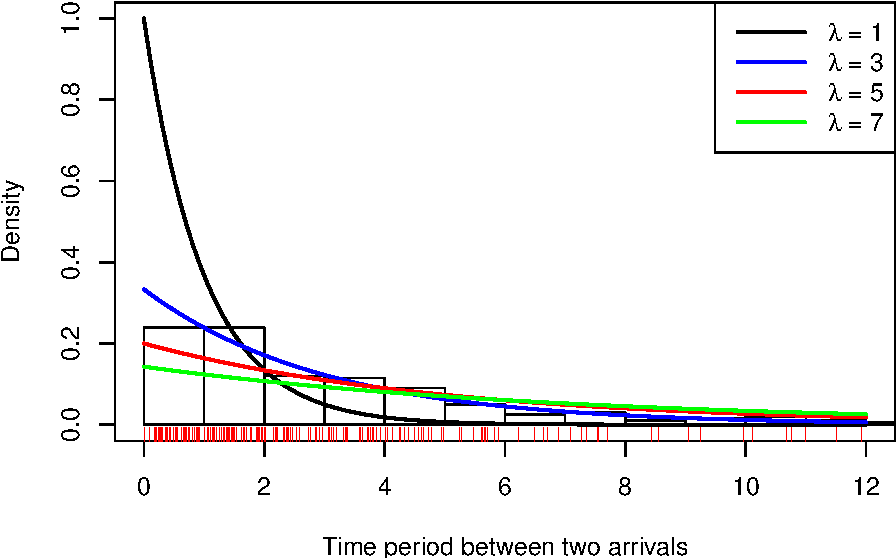
\includegraphics[width=0.95\linewidth]{EcoStat_files/figure-latex/MLE1-1} \caption{The red ticks, at the bottom, indicate observations (there are 200 of them). The historgram is based on these 200 observations}\label{fig:MLE1}
\end{figure}

What is your estimate of \(\lambda\)? Intuitively, one is led to take the \(\lambda\) for which the (theoretical) distribution is the closest to the histogram (that can be seen as an ``empirical distribution''). This approach is consistent with the idea of picking the \(\lambda\) for which the probability of observing the values included in \(\mathbf{y}\) is the highest.

Let us be more formal. Assume that you have only four observations: \(y_1=1.1\), \(y_2=2.2\), \(y_3=0.7\) and \(y_4=5.0\). What was the probability of jointly observing:

\begin{itemize}
\tightlist
\item
  \(1.1-\varepsilon \le Y_1 < 1.1+\varepsilon\),
\item
  \(2.2-\varepsilon \le Y_2 < 2.2+\varepsilon\),
\item
  \(0.7-\varepsilon \le Y_3 < 0.7+\varepsilon\), and
\item
  \(5.0-\varepsilon \le Y_4 < 5.0+\varepsilon\)?
\end{itemize}

Because the \(y_i\)'s are i.i.d., this probability is \(\prod_{i=1}^4(2\varepsilon f(y_i,\lambda))\).
The next plot shows the probability (divided by \(16\varepsilon^4\), which does not depend on \(\lambda\)) as a function of \(\lambda\).

\begin{figure}
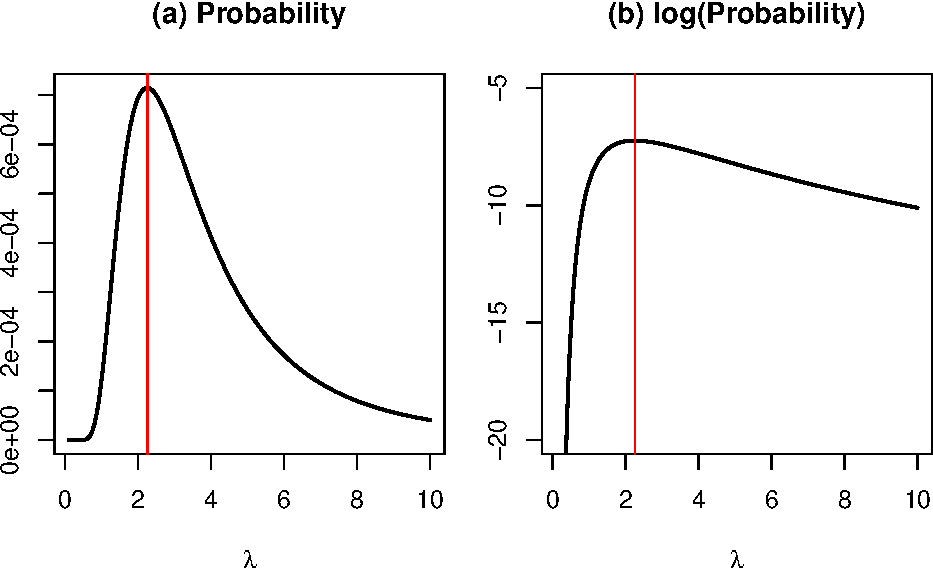
\includegraphics[width=0.95\linewidth]{EcoStat_files/figure-latex/MLE2-1} \caption{Proba. that $y_i-\varepsilon \le Y_i < y_i+\varepsilon$, $i \in \{1,2,3,4\}$. The vertical red line indicates the maximum of the function.}\label{fig:MLE2}
\end{figure}

The value of \(\lambda\) that maximizes the probability is 2.26.

Let us come back to the example with 200 observations:

\begin{figure}
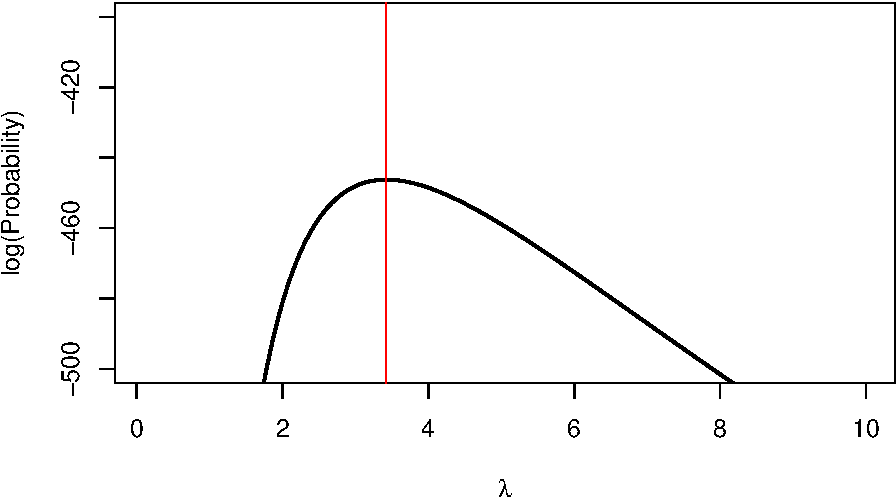
\includegraphics[width=0.95\linewidth]{EcoStat_files/figure-latex/MLE3-1} \caption{Log-likelihood function associated with the 200 i.i.d. observations. The vertical red line indicates the maximum of the function.}\label{fig:MLE3}
\end{figure}

In that case, the value of \(\lambda\) that maxmimizes the probability is 3.42.

\hypertarget{definition-and-properties}{%
\subsection{Definition and properties}\label{definition-and-properties}}

\(f(y;\boldsymbol\theta)\) denotes the probability density function (p.d.f.) of a random variable \(Y\) which depends on a set of parameters \(\boldsymbol\theta\). The density of \(n\) independent and identically distributed (i.i.d.) observations of \(Y\) is given by:
\[
f(\mathbf{y};\boldsymbol\theta) = \prod_{i=1}^n f(y_i;\boldsymbol\theta),
\]
where \(\mathbf{y}\) denotes the vector of observations; \(\mathbf{y} = \{y_1,\dots,y_n\}\).

\begin{definition}[Likelihood function]
\protect\hypertarget{def:likelihood}{}\label{def:likelihood}The likelihood function is:
\[
\mathcal{L}: \boldsymbol\theta \rightarrow  \mathcal{L}(\boldsymbol\theta;\mathbf{y})=f(\mathbf{y};\boldsymbol\theta)=f(y_1,\dots,y_n;\boldsymbol\theta).
\]
\end{definition}

We often work with \(\log \mathcal{L}\), the \textbf{log-likelihood function}.

\begin{example}[Gaussian distribution]
\protect\hypertarget{exm:normal}{}\label{exm:normal}If \(y_i \sim \mathcal{N}(\mu,\sigma^2)\), then
\[
\log \mathcal{L}(\boldsymbol\theta;\mathbf{y}) = - \frac{1}{2}\sum_{i=1}^n\left( \log \sigma^2 + \log 2\pi + \frac{(y_i-\mu)^2}{\sigma^2} \right).
\]
\end{example}

\begin{definition}[Score]
\protect\hypertarget{def:score}{}\label{def:score}The score \(S(y;\boldsymbol\theta)\) is given by \(\frac{\partial \log f(y;\boldsymbol\theta)}{\partial \boldsymbol\theta}\).
\end{definition}

If \(y_i \sim \mathcal{N}(\mu,\sigma^2)\) (Example \ref{exm:normal}), then
\[
\frac{\partial \log f(y;\boldsymbol\theta)}{\partial \boldsymbol\theta} =
\left[\begin{array}{c}
\dfrac{\partial \log f(y;\boldsymbol\theta)}{\partial \mu}\\
\dfrac{\partial \log f(y;\boldsymbol\theta)}{\partial \sigma^2}
\end{array}\right] =
\left[\begin{array}{c}
\dfrac{y-\mu}{\sigma^2}\\
\frac{1}{2\sigma^2}\left(\frac{(y-\mu)^2}{\sigma^2}-1\right)
\end{array}\right].
\]

\begin{proposition}[Score expectation]
\protect\hypertarget{prp:score}{}\label{prp:score}The expectation of the score is zero.
\end{proposition}

\begin{proof}
We have:
\begin{eqnarray*}
\mathbb{E}\left(\frac{\partial \log f(Y;\boldsymbol\theta)}{\partial \boldsymbol\theta}\right) &=&
\int \frac{\partial \log f(y;\boldsymbol\theta)}{\partial \boldsymbol\theta} f(y;\boldsymbol\theta) dy \\
&=& \int \frac{\partial f(y;\boldsymbol\theta)/\partial \boldsymbol\theta}{f(y;\boldsymbol\theta)} f(y;\boldsymbol\theta) dy =
\frac{\partial}{\partial \boldsymbol\theta} \int f(y;\boldsymbol\theta) dy\\
&=&\partial 1 /\partial \boldsymbol\theta = 0,
\end{eqnarray*}
which gives the result.
\end{proof}

\begin{definition}[Fisher information matrix]
\protect\hypertarget{def:Fisher}{}\label{def:Fisher}The information matrix is (minus) the the expectation of the second derivatives of the log-likelihood function:
\[
\mathcal{I}_Y(\boldsymbol\theta) = - \mathbb{E} \left( \frac{\partial^2 \log f(Y;\boldsymbol\theta)}{\partial \boldsymbol\theta \partial \boldsymbol\theta'} \right).
\]
\end{definition}

\begin{proposition}
\protect\hypertarget{prp:Fisher}{}\label{prp:Fisher}We have
\[
\mathcal{I}_Y(\boldsymbol\theta) = \mathbb{E} \left[ \left( \frac{\partial \log f(Y;\boldsymbol\theta)}{\partial \boldsymbol\theta} \right)
\left( \frac{\partial \log f(Y;\boldsymbol\theta)}{\partial \boldsymbol\theta} \right)' \right] = \mathbb{V}ar[S(Y;\boldsymbol\theta)].
\]
\end{proposition}

\begin{proof}
We have \(\frac{\partial^2 \log f(Y;\boldsymbol\theta)}{\partial \boldsymbol\theta \partial \boldsymbol\theta'} = \frac{\partial^2 f(Y;\boldsymbol\theta)}{\partial \boldsymbol\theta \partial \boldsymbol\theta'}\frac{1}{f(Y;\boldsymbol\theta)} - \frac{\partial \log f(Y;\boldsymbol\theta)}{\partial \boldsymbol\theta}\frac{\partial \log f(Y;\boldsymbol\theta)}{\partial \boldsymbol\theta'}\). The expectation of the first right-hand side term is \(\partial^2 1 /(\partial \boldsymbol\theta \partial \boldsymbol\theta') = \mathbf{0}\), which gives the result.
\end{proof}

\begin{example}
If \(y_i \sim\,i.i.d.\, \mathcal{N}(\mu,\sigma^2)\), let \(\boldsymbol\theta = [\mu,\sigma^2]'\) then
\[
\frac{\partial \log f(y;\boldsymbol\theta)}{\partial \boldsymbol\theta} = \left[\frac{y-\mu}{\sigma^2} \quad \frac{1}{2\sigma^2}\left(\frac{(y-\mu)^2}{\sigma^2}-1\right) \right]',
\]
and
\[
\mathcal{I}_Y(\boldsymbol\theta) = \mathbb{E}\left( \frac{1}{\sigma^4}
\left[
\begin{array}{cc}
\sigma^2&y-\mu\\
y-\mu & \frac{(y-\mu)^2}{\sigma^2}-\frac{1}{2}
\end{array}\right]
\right)=
\left[
\begin{array}{cc}
1/\sigma^2&0\\
0 & 1/(2\sigma^4)
\end{array}\right].
\]
\end{example}

\begin{proposition}[Additive property of the Information matrix]
\protect\hypertarget{prp:additiv}{}\label{prp:additiv}The information matrix resulting from two independent experiments is the sum of the information matrices:
\[
\mathcal{I}_{X,Y}(\boldsymbol\theta) = \mathcal{I}_X(\boldsymbol\theta) + \mathcal{I}_Y(\boldsymbol\theta).
\]
\end{proposition}

\begin{proof}
Directly deduced from the definition of the information matrix (Def. \ref{def:Fisher}), using that the epxectation of a product of independent variables is the product of the expectations.
\end{proof}

\begin{theorem}[Frechet-Darmois-Cramer-Rao bound]
\protect\hypertarget{thm:FDCR}{}\label{thm:FDCR}Consider an unbiased estimator of \(\boldsymbol\theta\) denoted by \(\hat{\boldsymbol\theta}(Y)\). The variance of the random variable \(\boldsymbol\omega'\hat{\boldsymbol\theta}\) (which is a linear combination of the components of \(\hat{\boldsymbol\theta}\)) is larger than:
\[
(\boldsymbol\omega'\boldsymbol\omega)^2/(\boldsymbol\omega' \mathcal{I}_Y(\boldsymbol\theta) \boldsymbol\omega).
\]
\end{theorem}

\begin{proof}
The Cauchy-Schwarz inequality implies that \(\sqrt{\mathbb{V}ar(\boldsymbol\omega'\hat{\boldsymbol\theta}(Y))\mathbb{V}ar(\boldsymbol\omega'S(Y;\boldsymbol\theta))} \ge |\boldsymbol\omega'\mathbb{C}ov[\hat{\boldsymbol\theta}(Y),S(Y;\boldsymbol\theta)]\boldsymbol\omega |\). Now, \(\mathbb{C}ov[\hat{\boldsymbol\theta}(Y),S(Y;\boldsymbol\theta)] = \int_y \hat{\boldsymbol\theta}(y) \frac{\partial \log f(y;\boldsymbol\theta)}{\partial \boldsymbol\theta} f(y;\boldsymbol\theta)dy = \frac{\partial}{\partial \boldsymbol\theta}\int_y \hat{\boldsymbol\theta}(y) f(y;\boldsymbol\theta)dy = \mathbf{I}\) because \(\hat{\boldsymbol\theta}\) is unbiased. Therefore \(\mathbb{V}ar(\boldsymbol\omega'\hat{\boldsymbol\theta}(Y)) \ge \mathbb{V}ar(\boldsymbol\omega'S(Y;\boldsymbol\theta))^{-1} (\boldsymbol\omega'\boldsymbol\omega)^2\). Prop. \ref{prp:Fisher} leads to the result.
\end{proof}

\begin{definition}[Identifiability]
\protect\hypertarget{def:identif}{}\label{def:identif}The vector of parameters \(\boldsymbol\theta\) is identifiable if, for any other vector \(\boldsymbol\theta^*\):
\[
\boldsymbol\theta^* \ne \boldsymbol\theta \Rightarrow \mathcal{L}(\boldsymbol\theta^*;\mathbf{y}) \ne \mathcal{L}(\boldsymbol\theta;\mathbf{y}).
\]
\end{definition}

\begin{definition}[Maximum Likelihood Estimator (MLE)]
\protect\hypertarget{def:MLEest}{}\label{def:MLEest}The maximum likelihood estimator (MLE) is the vector \(\boldsymbol\theta\) that maximizes the likelihood function. Formally:
\begin{equation}
\boldsymbol\theta_{MLE} = \arg \max_{\boldsymbol\theta} \mathcal{L}(\boldsymbol\theta;\mathbf{y})  = \arg \max_{\boldsymbol\theta} \log \mathcal{L}(\boldsymbol\theta;\mathbf{y}).\label{eq:MLEestimator}
\end{equation}
\end{definition}

\begin{definition}[Likelihood equation]
\protect\hypertarget{def:likFunction}{}\label{def:likFunction}A necessary condition for maximizing the likelihood function (under regularity assumption, see Hypotheses \ref{hyp:MLEregularity}) is:
\begin{equation}
\dfrac{\partial \log \mathcal{L}(\boldsymbol\theta;\mathbf{y})}{\partial \boldsymbol\theta} = \mathbf{0}.
\end{equation}
\end{definition}

\begin{hypothesis}[Regularity assumptions]
\protect\hypertarget{hyp:MLEregularity}{}\label{hyp:MLEregularity}

We have:

\begin{enumerate}
\def\labelenumi{\roman{enumi}.}
\tightlist
\item
  \(\boldsymbol\theta \in \Theta\) where \(\Theta\) is compact.
\item
  \(\boldsymbol\theta_0\) is identified.
\item
  The log-likelihood function is continuous in \(\boldsymbol\theta\).
\item
  \(\mathbb{E}_{\boldsymbol\theta_0}(\log f(Y;\boldsymbol\theta))\) exists.
\item
  The log-likelihood function is such that \((1/n)\log\mathcal{L}(\boldsymbol\theta;\mathbf{y})\) converges almost surely to \(\mathbb{E}_{\boldsymbol\theta_0}(\log f(Y;\boldsymbol\theta))\), uniformly in \(\boldsymbol\theta \in \Theta\).
\item
  The log-likelihood function is twice continuously differentiable in an open neighborood of \(\boldsymbol\theta_0\).
\item
  The matrix \(\mathbf{I}(\boldsymbol\theta_0) = - \mathbb{E}_0 \left( \frac{\partial^2 \log \mathcal{L}(\boldsymbol\theta;\mathbf{y})}{\partial \boldsymbol\theta \partial \boldsymbol\theta'}\right)\) ---the Fisher Information matrix--- exists and is nonsingular.
\end{enumerate}

\end{hypothesis}

\begin{proposition}[Properties of MLE]
\protect\hypertarget{prp:MLEproperties}{}\label{prp:MLEproperties}

Under regularity conditions (Assumptions \ref{hyp:MLEregularity}), the MLE is:

\begin{enumerate}
\def\labelenumi{\alph{enumi}.}
\tightlist
\item
  \textbf{Consistent}: \(\mbox{plim}\; \boldsymbol\theta_{MLE} = {\boldsymbol\theta}_0\) (\({\boldsymbol\theta}_0\) is the true vector of parameters).
\item
  \textbf{Asymptotically normal}:
  \begin{equation}
  \boxed{\sqrt{n}(\boldsymbol\theta_{MLE} - \boldsymbol\theta_{0}) \overset{d}{\rightarrow} \mathcal{N}(0,\mathcal{I}_Y(\boldsymbol\theta_0)^{-1}).} \label{eq:normMLE}
  \end{equation}
\item
  \textbf{Asymptotically efficient}: \(\boldsymbol\theta_{MLE}\) is asymptotically efficient and achieves the Freechet-Darmois-Cramer-Rao lower bound for consistent estimators.
\item
  \textbf{Invariant}: The MLE of \(g(\boldsymbol\theta_0)\) is \(g(\boldsymbol\theta_{MLE})\) if \(g\) is a continuous and continuously differentiable function.
\end{enumerate}

\end{proposition}

\begin{proof}
See Appendix \ref{AppendixProof}.
\end{proof}

Since \(\mathcal{I}_Y(\boldsymbol\theta_0)=\frac{1}{n}\mathbf{I}(\boldsymbol\theta_0)\), the asymptotic covariance matrix of the MLE is \([\mathbf{I}(\boldsymbol\theta_0)]^{-1}\), that is:
\[
[\mathbf{I}(\boldsymbol\theta_0)]^{-1} = \left[- \mathbb{E}_0 \left( \frac{\partial^2 \log \mathcal{L}(\boldsymbol\theta;\mathbf{y})}{\partial \boldsymbol\theta \partial \boldsymbol\theta'}\right) \right]^{-1}.
\]
A direct (analytical) evaluation of this expectation is often out of reach. It can however be estimated by, either:
\begin{eqnarray}
\hat{\mathbf{I}}_1^{-1} &=&  \left( - \frac{\partial^2 \log \mathcal{L}({\boldsymbol\theta_{MLE}};\mathbf{y})}{\partial {\boldsymbol\theta} \partial {\boldsymbol\theta}'}\right)^{-1}, \label{eq:III1}\\
\hat{\mathbf{I}}_2^{-1} &=&  \left( \sum_{i=1}^n \frac{\partial \log \mathcal{L}({\boldsymbol\theta_{MLE}};y_i)}{\partial {\boldsymbol\theta}} \frac{\partial \log \mathcal{L}({\boldsymbol\theta_{MLE}};y_i)}{\partial {\boldsymbol\theta'}} \right)^{-1}.  \label{eq:I2}
\end{eqnarray}

Asymptotically, we have \((\hat{\mathbf{I}}_1^{-1})\hat{\mathbf{I}}_2=Id\), that is, the two formulas provide the same result.

In case of (suspected) misspecification, one can use the so-called \emph{sandwich estimator} of the covariance matrix.\footnote{For more details, see, e.g., \href{https://www.stat.umn.edu/geyer/5601/notes/sand.pdf}{Charles Geyer's lectures notes}.} This covariance matrix is given by:
\begin{equation}
\hat{\mathbf{I}}_3^{-1} = \hat{\mathbf{I}}_2^{-1} \hat{\mathbf{I}}_1 \hat{\mathbf{I}}_2^{-1}.\label{eq:III3}
\end{equation}

\hypertarget{to-sum-up-mle-in-practice}{%
\subsection{To sum up -- MLE in practice}\label{to-sum-up-mle-in-practice}}

To implement MLE, we need:

\begin{itemize}
\tightlist
\item
  A parametric model (depending on the vector of parameters \(\boldsymbol\theta\) whose ``true'' value is \(\boldsymbol\theta_0\)) is specified.
\item
  i.i.d. sources of randomness are identified.
\item
  The density associated to one observation \(y_i\) is computed analytically (as a function of \(\boldsymbol\theta\)): \(f(y;\boldsymbol\theta)\).
\item
  The log-likelihood is \(\log \mathcal{L}(\boldsymbol\theta;\mathbf{y}) = \sum_i \log f(y_i;\boldsymbol\theta)\).
\item
  The MLE estimator results from the optimization problem (this is Eq. \eqref{eq:MLEestimator}):
  \begin{equation}
  \boldsymbol\theta_{MLE} = \arg \max_{\boldsymbol\theta} \log \mathcal{L}(\boldsymbol\theta;\mathbf{y}).
  \end{equation}
\item
  We have: \(\boldsymbol\theta_{MLE} \sim \mathcal{N}({\boldsymbol\theta}_0,\mathbf{I}(\boldsymbol\theta_0)^{-1})\), where \(\mathbf{I}(\boldsymbol\theta_0)^{-1}\) is estimated by means of Eq. \eqref{eq:III1}, Eq. \eqref{eq:I2}, or Eq. \eqref{eq:III3}. Most of the time, this computation is numerical.
\end{itemize}

\hypertarget{example-mle-estimation-of-a-mixture-of-gaussian-distribution}{%
\subsection{Example: MLE estimation of a mixture of Gaussian distribution}\label{example-mle-estimation-of-a-mixture-of-gaussian-distribution}}

Consider the returns of the Swiss Market Index (SMI). Assume that these returns are independently drawn from a mixture of Gaussian distributions. The p.d.f. \(f(x;\boldsymbol\theta)\), with \(\boldsymbol\theta = [\mu_1,\sigma_1,\mu_2,\sigma_2,p]'\), is given by:
\[
p \frac{1}{\sqrt{2\pi\sigma_1^2}}\exp\left(-\frac{(x - \mu_1)^2}{2\sigma_1^2}\right) + (1-p)\frac{1}{\sqrt{2\pi\sigma_2^2}}\exp\left(-\frac{(x - \mu_2)^2}{2\sigma_2^2}\right).
\]
(See \href{https://jrenne.shinyapps.io/density/}{p.d.f. of mixtures of Gaussian distributions}.)

\begin{Shaded}
\begin{Highlighting}[]
\FunctionTok{library}\NormalTok{(AEC);}\FunctionTok{data}\NormalTok{(smi)}
\NormalTok{T }\OtherTok{\textless{}{-}} \FunctionTok{dim}\NormalTok{(smi)[}\DecValTok{1}\NormalTok{]}
\NormalTok{h }\OtherTok{\textless{}{-}} \DecValTok{5} \CommentTok{\# holding period (one week)}
\NormalTok{smi}\SpecialCharTok{$}\NormalTok{r }\OtherTok{\textless{}{-}} \FunctionTok{c}\NormalTok{(}\FunctionTok{rep}\NormalTok{(}\ConstantTok{NaN}\NormalTok{,h),}
           \DecValTok{100}\SpecialCharTok{*}\FunctionTok{c}\NormalTok{(}\FunctionTok{log}\NormalTok{(smi}\SpecialCharTok{$}\NormalTok{Close[(}\DecValTok{1}\SpecialCharTok{+}\NormalTok{h)}\SpecialCharTok{:}\NormalTok{T]}\SpecialCharTok{/}\NormalTok{smi}\SpecialCharTok{$}\NormalTok{Close[}\DecValTok{1}\SpecialCharTok{:}\NormalTok{(T}\SpecialCharTok{{-}}\NormalTok{h)])))}
\NormalTok{indic.dates }\OtherTok{\textless{}{-}} \FunctionTok{seq}\NormalTok{(}\DecValTok{1}\NormalTok{,T,}\AttributeTok{by=}\DecValTok{5}\NormalTok{)  }\CommentTok{\# weekly returns}
\NormalTok{smi }\OtherTok{\textless{}{-}}\NormalTok{ smi[indic.dates,]}
\NormalTok{smi }\OtherTok{\textless{}{-}}\NormalTok{ smi[}\FunctionTok{complete.cases}\NormalTok{(smi),]}
\FunctionTok{par}\NormalTok{(}\AttributeTok{mfrow=}\FunctionTok{c}\NormalTok{(}\DecValTok{1}\NormalTok{,}\DecValTok{1}\NormalTok{));}\FunctionTok{par}\NormalTok{(}\AttributeTok{plt=}\FunctionTok{c}\NormalTok{(.}\DecValTok{15}\NormalTok{,.}\DecValTok{95}\NormalTok{,.}\DecValTok{1}\NormalTok{,.}\DecValTok{95}\NormalTok{))}
\FunctionTok{plot}\NormalTok{(smi}\SpecialCharTok{$}\NormalTok{Date,smi}\SpecialCharTok{$}\NormalTok{r,}\AttributeTok{type=}\StringTok{"l"}\NormalTok{,}\AttributeTok{xlab=}\StringTok{""}\NormalTok{,}\AttributeTok{ylab=}\StringTok{"in percent"}\NormalTok{)}
\FunctionTok{abline}\NormalTok{(}\AttributeTok{h=}\DecValTok{0}\NormalTok{,}\AttributeTok{col=}\StringTok{"blue"}\NormalTok{)}
\FunctionTok{abline}\NormalTok{(}\AttributeTok{h=}\FunctionTok{mean}\NormalTok{(smi}\SpecialCharTok{$}\NormalTok{r,}\AttributeTok{na.rm =} \ConstantTok{TRUE}\NormalTok{)}\SpecialCharTok{+}\DecValTok{2}\SpecialCharTok{*}\FunctionTok{sd}\NormalTok{(smi}\SpecialCharTok{$}\NormalTok{r,}\AttributeTok{na.rm =} \ConstantTok{TRUE}\NormalTok{),}\AttributeTok{lty=}\DecValTok{3}\NormalTok{,}\AttributeTok{col=}\StringTok{"blue"}\NormalTok{)}
\FunctionTok{abline}\NormalTok{(}\AttributeTok{h=}\FunctionTok{mean}\NormalTok{(smi}\SpecialCharTok{$}\NormalTok{r,}\AttributeTok{na.rm =} \ConstantTok{TRUE}\NormalTok{)}\SpecialCharTok{{-}}\DecValTok{2}\SpecialCharTok{*}\FunctionTok{sd}\NormalTok{(smi}\SpecialCharTok{$}\NormalTok{r,}\AttributeTok{na.rm =} \ConstantTok{TRUE}\NormalTok{),}\AttributeTok{lty=}\DecValTok{3}\NormalTok{,}\AttributeTok{col=}\StringTok{"blue"}\NormalTok{)}
\end{Highlighting}
\end{Shaded}

\begin{figure}
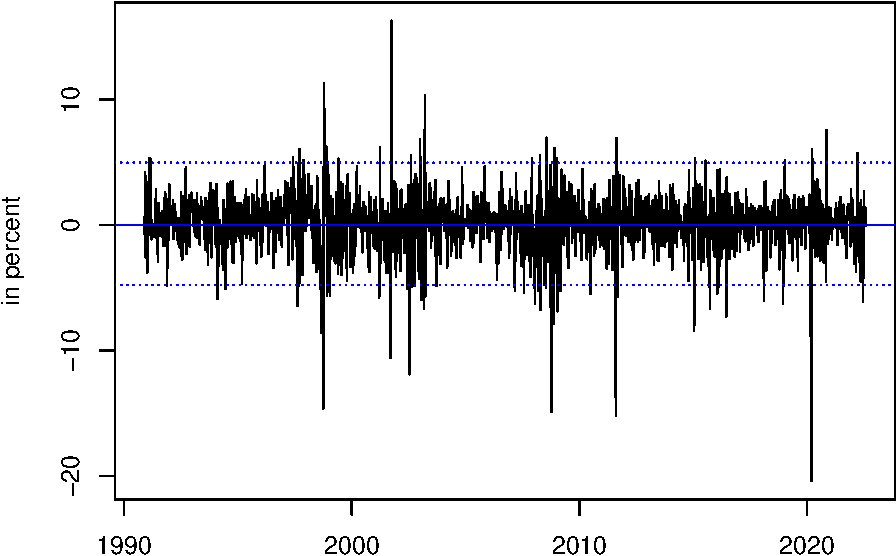
\includegraphics[width=0.95\linewidth]{EcoStat_files/figure-latex/smiData-1} \caption{Time series of SMI weekly returns (source: Yahoo Finance).}\label{fig:smiData}
\end{figure}

Build the log-likelihood function (fucntion \texttt{log.f}), and use the numerical BFGS algorithm to maximize it (using the \texttt{optim} wrapper):

\begin{Shaded}
\begin{Highlighting}[]
\NormalTok{f }\OtherTok{\textless{}{-}} \ControlFlowTok{function}\NormalTok{(theta,y)\{ }\CommentTok{\# Likelihood function}
\NormalTok{  mu}\FloatTok{.1} \OtherTok{\textless{}{-}}\NormalTok{ theta[}\DecValTok{1}\NormalTok{]; mu}\FloatTok{.2} \OtherTok{\textless{}{-}}\NormalTok{ theta[}\DecValTok{2}\NormalTok{]}
\NormalTok{  sigma}\FloatTok{.1} \OtherTok{\textless{}{-}}\NormalTok{ theta[}\DecValTok{3}\NormalTok{]; sigma}\FloatTok{.2} \OtherTok{\textless{}{-}}\NormalTok{ theta[}\DecValTok{4}\NormalTok{]}
\NormalTok{  p }\OtherTok{\textless{}{-}} \FunctionTok{exp}\NormalTok{(theta[}\DecValTok{5}\NormalTok{])}\SpecialCharTok{/}\NormalTok{(}\DecValTok{1}\SpecialCharTok{+}\FunctionTok{exp}\NormalTok{(theta[}\DecValTok{5}\NormalTok{]))}
\NormalTok{  res }\OtherTok{\textless{}{-}}\NormalTok{ p}\SpecialCharTok{*}\DecValTok{1}\SpecialCharTok{/}\FunctionTok{sqrt}\NormalTok{(}\DecValTok{2}\SpecialCharTok{*}\NormalTok{pi}\SpecialCharTok{*}\NormalTok{sigma}\FloatTok{.1}\SpecialCharTok{\^{}}\DecValTok{2}\NormalTok{)}\SpecialCharTok{*}\FunctionTok{exp}\NormalTok{(}\SpecialCharTok{{-}}\NormalTok{(y}\SpecialCharTok{{-}}\NormalTok{mu}\FloatTok{.1}\NormalTok{)}\SpecialCharTok{\^{}}\DecValTok{2}\SpecialCharTok{/}\NormalTok{(}\DecValTok{2}\SpecialCharTok{*}\NormalTok{sigma}\FloatTok{.1}\SpecialCharTok{\^{}}\DecValTok{2}\NormalTok{)) }\SpecialCharTok{+}
\NormalTok{    (}\DecValTok{1}\SpecialCharTok{{-}}\NormalTok{p)}\SpecialCharTok{*}\DecValTok{1}\SpecialCharTok{/}\FunctionTok{sqrt}\NormalTok{(}\DecValTok{2}\SpecialCharTok{*}\NormalTok{pi}\SpecialCharTok{*}\NormalTok{sigma}\FloatTok{.2}\SpecialCharTok{\^{}}\DecValTok{2}\NormalTok{)}\SpecialCharTok{*}\FunctionTok{exp}\NormalTok{(}\SpecialCharTok{{-}}\NormalTok{(y}\SpecialCharTok{{-}}\NormalTok{mu}\FloatTok{.2}\NormalTok{)}\SpecialCharTok{\^{}}\DecValTok{2}\SpecialCharTok{/}\NormalTok{(}\DecValTok{2}\SpecialCharTok{*}\NormalTok{sigma}\FloatTok{.2}\SpecialCharTok{\^{}}\DecValTok{2}\NormalTok{))}
  \FunctionTok{return}\NormalTok{(res)}
\NormalTok{\}}
\NormalTok{log.f }\OtherTok{\textless{}{-}} \ControlFlowTok{function}\NormalTok{(theta,y)\{ }\CommentTok{\#log{-}Likelihood function}
  \FunctionTok{return}\NormalTok{(}\SpecialCharTok{{-}}\FunctionTok{sum}\NormalTok{(}\FunctionTok{log}\NormalTok{(}\FunctionTok{f}\NormalTok{(theta,y))))}
\NormalTok{\}}
\NormalTok{res.optim }\OtherTok{\textless{}{-}} \FunctionTok{optim}\NormalTok{(}\FunctionTok{c}\NormalTok{(}\DecValTok{0}\NormalTok{,}\DecValTok{0}\NormalTok{,}\FloatTok{0.5}\NormalTok{,}\FloatTok{1.5}\NormalTok{,.}\DecValTok{5}\NormalTok{),}
\NormalTok{                   log.f,}
                   \AttributeTok{y=}\NormalTok{smi}\SpecialCharTok{$}\NormalTok{r,}
                   \AttributeTok{method=}\StringTok{"BFGS"}\NormalTok{, }\CommentTok{\# could be "Nelder{-}Mead"}
                   \AttributeTok{control=}\FunctionTok{list}\NormalTok{(}\AttributeTok{trace=}\ConstantTok{FALSE}\NormalTok{,}\AttributeTok{maxit=}\DecValTok{100}\NormalTok{),}\AttributeTok{hessian=}\ConstantTok{TRUE}\NormalTok{)}
\NormalTok{theta }\OtherTok{\textless{}{-}}\NormalTok{ res.optim}\SpecialCharTok{$}\NormalTok{par}
\NormalTok{theta}
\end{Highlighting}
\end{Shaded}

\begin{verbatim}
## [1]  0.3012379 -1.3167476  1.7715072  4.8197596  1.9454889
\end{verbatim}

Next, compute estimates of the covariance matrix of the MLE (using Eqs. \eqref{eq:III1}, \eqref{eq:I2}, and \eqref{eq:III3}), and compare the three sets of resulting standard deviations for the five estimated paramters:

\begin{Shaded}
\begin{Highlighting}[]
\CommentTok{\# Hessian approach:}
\NormalTok{I}\FloatTok{.1} \OtherTok{\textless{}{-}} \FunctionTok{solve}\NormalTok{(res.optim}\SpecialCharTok{$}\NormalTok{hessian)}
\CommentTok{\# Outer{-}product of gradient approach:}
\NormalTok{log.f}\FloatTok{.0} \OtherTok{\textless{}{-}} \FunctionTok{log}\NormalTok{(}\FunctionTok{f}\NormalTok{(theta,smi}\SpecialCharTok{$}\NormalTok{r))}
\NormalTok{epsilon }\OtherTok{\textless{}{-}}\NormalTok{ .}\DecValTok{00000001}
\NormalTok{d.log.f }\OtherTok{\textless{}{-}} \ConstantTok{NULL}
\ControlFlowTok{for}\NormalTok{(i }\ControlFlowTok{in} \DecValTok{1}\SpecialCharTok{:}\FunctionTok{length}\NormalTok{(theta))\{}
\NormalTok{  theta.i }\OtherTok{\textless{}{-}}\NormalTok{ theta}
\NormalTok{  theta.i[i] }\OtherTok{\textless{}{-}}\NormalTok{ theta.i[i] }\SpecialCharTok{+}\NormalTok{ epsilon}
\NormalTok{  log.f.i }\OtherTok{\textless{}{-}} \FunctionTok{log}\NormalTok{(}\FunctionTok{f}\NormalTok{(theta.i,smi}\SpecialCharTok{$}\NormalTok{r))}
\NormalTok{  d.log.f }\OtherTok{\textless{}{-}} \FunctionTok{cbind}\NormalTok{(d.log.f,}
\NormalTok{                   (log.f.i }\SpecialCharTok{{-}}\NormalTok{ log.f}\FloatTok{.0}\NormalTok{)}\SpecialCharTok{/}\NormalTok{epsilon)}
\NormalTok{\}}
\NormalTok{I}\FloatTok{.2} \OtherTok{\textless{}{-}} \FunctionTok{solve}\NormalTok{(}\FunctionTok{t}\NormalTok{(d.log.f) }\SpecialCharTok{\%*\%}\NormalTok{ d.log.f)}
\CommentTok{\# Misspecification{-}robust approach (sandwich formula):}
\NormalTok{I}\FloatTok{.3} \OtherTok{\textless{}{-}}\NormalTok{ I}\FloatTok{.1} \SpecialCharTok{\%*\%} \FunctionTok{solve}\NormalTok{(I}\FloatTok{.2}\NormalTok{) }\SpecialCharTok{\%*\%}\NormalTok{ I}\FloatTok{.1}
\FunctionTok{cbind}\NormalTok{(}\FunctionTok{diag}\NormalTok{(I}\FloatTok{.1}\NormalTok{),}\FunctionTok{diag}\NormalTok{(I}\FloatTok{.2}\NormalTok{),}\FunctionTok{diag}\NormalTok{(I}\FloatTok{.3}\NormalTok{))}
\end{Highlighting}
\end{Shaded}

\begin{verbatim}
##             [,1]        [,2]       [,3]
## [1,] 0.003683422 0.003199481 0.00586160
## [2,] 0.226892824 0.194283391 0.38653389
## [3,] 0.005764271 0.002769579 0.01712255
## [4,] 0.194081311 0.047466419 0.83130838
## [5,] 0.092114437 0.040366005 0.31347858
\end{verbatim}

According to the first (respectively third) type of estimate for the covariance matrix, a 95\% confidence interval for \(\mu_1\) is {[}0.182, 0.42{]} (resp. {[}0.151, 0.451{]}).

Note that we have not directly estimated parameter \(p\) but \(\nu = \log(p/(1-p))\) (in such a way that \(p = \exp(\nu)/(1+\exp(\nu))\)). In order to get an estimate of the standard deviation of our esitmate of \(p\), we can implement the \textbf{Delta method}. This method is based on the fact that, for a function \(g\) that is continuous in the neighborhood of \(\boldsymbol\theta_0\) and for large \(n\), we have:
\begin{equation}
\mathbb{V}ar(g(\hat{\boldsymbol\theta}_n)) \approx \frac{\partial g(\hat{\boldsymbol\theta}_n)}{\partial \boldsymbol\theta'}\mathbb{V}ar(\hat{\boldsymbol\theta}_n)\frac{\partial g(\hat{\boldsymbol\theta}_n)'}{\partial \boldsymbol\theta}.\label{eq:DeltaMethod}
\end{equation}

\begin{Shaded}
\begin{Highlighting}[]
\NormalTok{g }\OtherTok{\textless{}{-}} \ControlFlowTok{function}\NormalTok{(theta)\{}
\NormalTok{  mu}\FloatTok{.1} \OtherTok{\textless{}{-}}\NormalTok{ theta[}\DecValTok{1}\NormalTok{]; mu}\FloatTok{.2} \OtherTok{\textless{}{-}}\NormalTok{ theta[}\DecValTok{2}\NormalTok{]}
\NormalTok{  sigma}\FloatTok{.1} \OtherTok{\textless{}{-}}\NormalTok{ theta[}\DecValTok{3}\NormalTok{]; sigma}\FloatTok{.2} \OtherTok{\textless{}{-}}\NormalTok{ theta[}\DecValTok{4}\NormalTok{]}
\NormalTok{  p }\OtherTok{\textless{}{-}} \FunctionTok{exp}\NormalTok{(theta[}\DecValTok{5}\NormalTok{])}\SpecialCharTok{/}\NormalTok{(}\DecValTok{1}\SpecialCharTok{+}\FunctionTok{exp}\NormalTok{(theta[}\DecValTok{5}\NormalTok{]))}
  \FunctionTok{return}\NormalTok{(}\FunctionTok{c}\NormalTok{(mu}\FloatTok{.1}\NormalTok{,mu}\FloatTok{.2}\NormalTok{,sigma}\FloatTok{.1}\NormalTok{,sigma}\FloatTok{.2}\NormalTok{,p))}
\NormalTok{\}}
\CommentTok{\# Computation of g\textquotesingle{}s gradient around estimated theta:}
\NormalTok{eps }\OtherTok{\textless{}{-}}\NormalTok{ .}\DecValTok{00001}
\NormalTok{g.theta }\OtherTok{\textless{}{-}} \FunctionTok{g}\NormalTok{(theta)}
\NormalTok{g.gradient }\OtherTok{\textless{}{-}} \ConstantTok{NULL}
\ControlFlowTok{for}\NormalTok{(i }\ControlFlowTok{in} \DecValTok{1}\SpecialCharTok{:}\DecValTok{5}\NormalTok{)\{}
\NormalTok{  theta.perturb }\OtherTok{\textless{}{-}}\NormalTok{ theta}
\NormalTok{  theta.perturb[i] }\OtherTok{\textless{}{-}}\NormalTok{ theta[i] }\SpecialCharTok{+}\NormalTok{ eps}
\NormalTok{  g.gradient }\OtherTok{\textless{}{-}} \FunctionTok{cbind}\NormalTok{(g.gradient,(}\FunctionTok{g}\NormalTok{(theta.perturb)}\SpecialCharTok{{-}}\NormalTok{g.theta)}\SpecialCharTok{/}\NormalTok{eps)}
\NormalTok{\}}
\NormalTok{Var }\OtherTok{\textless{}{-}}\NormalTok{ g.gradient }\SpecialCharTok{\%*\%}\NormalTok{ I}\FloatTok{.3} \SpecialCharTok{\%*\%} \FunctionTok{t}\NormalTok{(g.gradient)}
\NormalTok{stdv.g.theta }\OtherTok{\textless{}{-}} \FunctionTok{sqrt}\NormalTok{(}\FunctionTok{diag}\NormalTok{(Var))}
\NormalTok{stdv.theta }\OtherTok{\textless{}{-}} \FunctionTok{sqrt}\NormalTok{(}\FunctionTok{diag}\NormalTok{(I}\FloatTok{.3}\NormalTok{))}
\FunctionTok{cbind}\NormalTok{(theta,stdv.theta,g.theta,stdv.g.theta)}
\end{Highlighting}
\end{Shaded}

\begin{verbatim}
##           theta stdv.theta    g.theta stdv.g.theta
## [1,]  0.3012379 0.07656108  0.3012379   0.07656108
## [2,] -1.3167476 0.62171850 -1.3167476   0.62171850
## [3,]  1.7715072 0.13085316  1.7715072   0.13085316
## [4,]  4.8197596 0.91176114  4.8197596   0.91176114
## [5,]  1.9454889 0.55989158  0.8749539   0.06125726
\end{verbatim}

The previous results show that the MLE estimate of \(p\) is 0.8749539, and its standard deviation is approximately equal to 0.0612573.

To finish with, let us draw the estimated parametric p.d.f. (the mixture of Gaussian distribution), and compare it to a non-parametric (kernel-based) estimate of this p.d.f. (using function \texttt{density}):

\begin{Shaded}
\begin{Highlighting}[]
\NormalTok{x }\OtherTok{\textless{}{-}} \FunctionTok{seq}\NormalTok{(}\SpecialCharTok{{-}}\DecValTok{5}\NormalTok{,}\DecValTok{5}\NormalTok{,}\AttributeTok{by=}\NormalTok{.}\DecValTok{01}\NormalTok{)}
\FunctionTok{par}\NormalTok{(}\AttributeTok{plt=}\FunctionTok{c}\NormalTok{(.}\DecValTok{1}\NormalTok{,.}\DecValTok{95}\NormalTok{,.}\DecValTok{1}\NormalTok{,.}\DecValTok{95}\NormalTok{))}
\FunctionTok{plot}\NormalTok{(x,}\FunctionTok{f}\NormalTok{(theta,x),}\AttributeTok{type=}\StringTok{"l"}\NormalTok{,}\AttributeTok{lwd=}\DecValTok{2}\NormalTok{,}\AttributeTok{xlab=}\StringTok{"returns, in percent"}\NormalTok{,}\AttributeTok{ylab=}\StringTok{""}\NormalTok{,}
     \AttributeTok{ylim=}\FunctionTok{c}\NormalTok{(}\DecValTok{0}\NormalTok{,}\FloatTok{1.4}\SpecialCharTok{*}\FunctionTok{max}\NormalTok{(}\FunctionTok{f}\NormalTok{(theta,x))))}
\FunctionTok{lines}\NormalTok{(}\FunctionTok{density}\NormalTok{(smi}\SpecialCharTok{$}\NormalTok{r),}\AttributeTok{type=}\StringTok{"l"}\NormalTok{,}\AttributeTok{lwd=}\DecValTok{2}\NormalTok{,}\AttributeTok{lty=}\DecValTok{3}\NormalTok{)}
\FunctionTok{lines}\NormalTok{(x,}\FunctionTok{dnorm}\NormalTok{(x,}\AttributeTok{mean=}\FunctionTok{mean}\NormalTok{(smi}\SpecialCharTok{$}\NormalTok{r),}\AttributeTok{sd =} \FunctionTok{sd}\NormalTok{(smi}\SpecialCharTok{$}\NormalTok{r)),}\AttributeTok{col=}\StringTok{"red"}\NormalTok{,}\AttributeTok{lty=}\DecValTok{2}\NormalTok{,}\AttributeTok{lwd=}\DecValTok{2}\NormalTok{)}
\FunctionTok{rug}\NormalTok{(smi}\SpecialCharTok{$}\NormalTok{r,}\AttributeTok{col=}\StringTok{"blue"}\NormalTok{)}
\FunctionTok{legend}\NormalTok{(}\StringTok{"topleft"}\NormalTok{,}
       \FunctionTok{c}\NormalTok{(}\StringTok{"Kernel estimate (non{-}parametric)"}\NormalTok{,}
         \StringTok{"Estimated mixture of Gaussian distr. (MLE, parametric)"}\NormalTok{,}
         \StringTok{"Normal distribution"}\NormalTok{),}
       \AttributeTok{lty=}\FunctionTok{c}\NormalTok{(}\DecValTok{3}\NormalTok{,}\DecValTok{1}\NormalTok{,}\DecValTok{2}\NormalTok{),}\AttributeTok{lwd=}\FunctionTok{c}\NormalTok{(}\DecValTok{2}\NormalTok{), }\CommentTok{\# line width}
       \AttributeTok{col=}\FunctionTok{c}\NormalTok{(}\StringTok{"black"}\NormalTok{,}\StringTok{"black"}\NormalTok{,}\StringTok{"red"}\NormalTok{),}\AttributeTok{pt.bg=}\FunctionTok{c}\NormalTok{(}\DecValTok{1}\NormalTok{),}\AttributeTok{pt.cex =} \FunctionTok{c}\NormalTok{(}\DecValTok{1}\NormalTok{),}
       \AttributeTok{bg=}\StringTok{"white"}\NormalTok{,}\AttributeTok{seg.len =} \DecValTok{4}\NormalTok{)}
\end{Highlighting}
\end{Shaded}

\begin{figure}
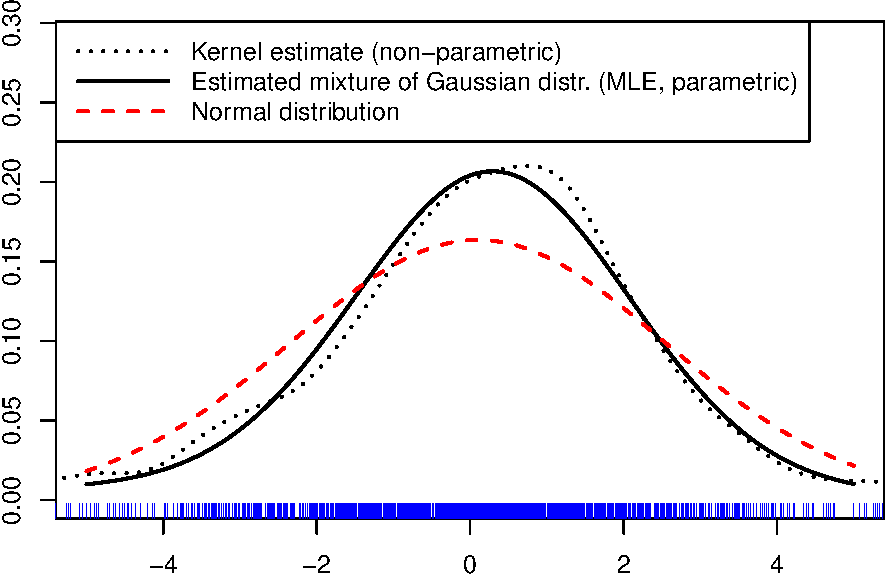
\includegraphics[width=0.95\linewidth]{EcoStat_files/figure-latex/smidistri-1} \caption{Comparison of different estimates of the distribution of returns.}\label{fig:smidistri}
\end{figure}

\hypertarget{TestMLE}{%
\subsection{Test procedures}\label{TestMLE}}

Suppose we want to test the following parameter restrictions:
\begin{equation}
\boxed{H_0: \underbrace{h(\boldsymbol\theta)}_{r \times 1}=0.}
\end{equation}

In the context of MLE, three tests are largely used:

\begin{itemize}
\tightlist
\item
  Likelihood Ratio (LR) test,
\item
  Wald (W) test,
\item
  Lagrange Multiplier (LM) test.
\end{itemize}

Here is the rationale behind these three tests:\footnote{An interesting graphical presentation of the tests is proposed in \href{http://hedibert.org/wp-content/uploads/2014/04/LR-W-LM-Tests-Buse1982.pdf}{Buse (1982)}.}

\begin{itemize}
\tightlist
\item
  LR: If \(h(\boldsymbol\theta)=0\), then imposing this restriction during the estimation (restricted estimator) should not result in a large decrease in the likelihood function (w.r.t the unrestricted estimation).
\item
  Wald: If \(h(\boldsymbol\theta)=0\), then \(h(\hat{\boldsymbol\theta})\) should not be far from \(0\) (even if these restrictions are not imposed during the MLE).
\item
  LM: If \(h(\boldsymbol\theta)=0\), then the gradient of the likelihood function should be small when evaluated at the restricted estimator.
\end{itemize}

In terms of implementation, while the LR necessitates to estimate both restricted and unrestricted models, the Wald test requires the estimation of the unrestricted model only, and the LM tests requires the estimation of the restricted model only.

As shown below, the three test statistics associated with these three tests coincide asymptotically. (Therefore, they naturally have the same asymptotic distribution, that are \(\chi^2\).)

\begin{proposition}[Asymptotic distribution of the Wald statistic]
\protect\hypertarget{prp:Walddistri}{}\label{prp:Walddistri}Under regularity conditions (Assumptions \ref{hyp:MLEregularity}) and under \(H_0: h(\boldsymbol\theta)=0\), the Wald statistic, defined by:
\[
\boxed{\xi^W = h(\hat{\boldsymbol\theta})' \mathbb{V}ar[h(\hat{\boldsymbol\theta})]^{-1} h(\hat{\boldsymbol\theta}),}
\]
where
\begin{equation}
\mathbb{V}ar[h(\hat{\boldsymbol\theta})] = \left(\frac{\partial h(\hat{\boldsymbol\theta})}{\partial \boldsymbol\theta'} \right) \mathbb{V}ar[\hat{\boldsymbol\theta}]
\left(\frac{\partial h(\hat{\boldsymbol\theta})'}{\partial \boldsymbol\theta} \right),\label{eq:varinWald}
\end{equation}
is asymptotically \(\chi^2(r)\), where the number of degrees of freedom \(r\) corresponds to the dimension of \(h(\boldsymbol\theta)\). (Note that Eq. \eqref{eq:varinWald} is the same as the one used in the Delta method, see Eq. \eqref{eq:DeltaMethod}.)

The Wald test, defined by the critical region
\[
\{\xi^W \ge \chi^2_{1-\alpha}(r)\},
\]
where \(\chi^2_{1-\alpha}(r)\) denotes the quantile of level \(1-\alpha\) of the \(\chi^2(r)\) distribution, has asymptotic level \(\alpha\) and is consistent.\footnote{See Defs. \ref{def:asmyptlevel} and \ref{def:asmyptconsisttest} for definitions of the asymptotic levels and consistency of tests.}
\end{proposition}

\begin{proof}
See Appendix \ref{AppendixProof}.
\end{proof}

In practice, in Eq. \eqref{eq:varinWald}, \(\mathbb{V}ar[\hat{\boldsymbol\theta}]\) is replaced by an estimate given, e.g., by Eq. \eqref{eq:III1}, Eq. \eqref{eq:I2}, or Eq. \eqref{eq:III3}.

\begin{proposition}[Asymptotic distribution of the LM test statistic]
\protect\hypertarget{prp:LMdistri}{}\label{prp:LMdistri}Under regularity conditions (Assumptions \ref{hyp:MLEregularity}) and under \(H_0: h(\boldsymbol\theta)=0\), the LM statistic
\begin{equation}
\boxed{\xi^{LM} =
\left(\left.\frac{\partial \log \mathcal{L}(\boldsymbol\theta)}{\partial \boldsymbol\theta'}\right|_{\boldsymbol\theta = \hat{\boldsymbol\theta}^0}  \right)
[\mathbf{I}(\hat{\boldsymbol\theta}^0)]^{-1}
\left(\left.\frac{\partial \log \mathcal{L}(\boldsymbol\theta)}{\partial \boldsymbol\theta }\right|_{\boldsymbol\theta = \hat{\boldsymbol\theta}^0}  \right),} \label{eq:xiLM}
\end{equation}
(where \(\hat{\boldsymbol\theta}^0\) is the restricted MLE estimator) is \(\chi^2(r)\).

The test defined by the critical region:
\[
\{\xi^{LM} \ge \chi^2_{1-\alpha}(r)\}
\]
has asymptotic level \(\alpha\) and is consistent (see Defs. \ref{def:asmyptlevel} and \ref{def:asmyptconsisttest}). This test is called \emph{Score} or \emph{Lagrange Multiplier (LM)} test.
\end{proposition}

\begin{proof}
See Appendix \ref{AppendixProof}.
\end{proof}

\begin{definition}[Likelihood Ratio test statistics]
\protect\hypertarget{def:LR}{}\label{def:LR}The likelihood ratio associated to a restriction of the form \(H_0: h({\boldsymbol\theta})=0\) is given by:
\[
LR = \frac{\mathcal{L}_R(\boldsymbol\theta;\mathbf{y})}{\mathcal{L}_U(\boldsymbol\theta;\mathbf{y})} \quad (\in [0,1]),
\]
where \(\mathcal{L}_R\) (respectively \(\mathcal{L}_U\)) is the likelihood function that imposes (resp. that does not impose) the restriction. The likelihood ratio test statistic is given by \(-2\log(LR)\), that is:
\[
\boxed{\xi^{LR}= 2 (\log\mathcal{L}_U(\boldsymbol\theta;\mathbf{y})-\log\mathcal{L}_R(\boldsymbol\theta;\mathbf{y})).}
\]
\end{definition}

\begin{proposition}[Asymptotic equivalence of LR, LM, and Wald tests]
\protect\hypertarget{prp:equivLRLMW}{}\label{prp:equivLRLMW}Under the null hypothesis \(H_0\), we have, asymptotically:
\[
\xi^{LM} = \xi^{LR} = \xi^{W}.
\]
\end{proposition}

\begin{proof}
See Appendix \ref{AppendixProof}.
\end{proof}

\hypertarget{bayesian-approach}{%
\section{Bayesian approach}\label{bayesian-approach}}

\hypertarget{introduction}{%
\subsection{Introduction}\label{introduction}}

An excellent introduction to Bayesian methods is proposed by \href{http://www.columbia.edu/~mh2078/MonteCarlo/MCMC_Bayes.pdf}{Martin Haugh, 2017}.

As suggested by the name of this approach, the starting point is the Bayes formula:
\[
\mathbb{P}(A|B) = \frac{\mathbb{P}(A \& B)}{\mathbb{P}(B)},
\]
where \(A\) and \(B\) are two ``events''. For instance, \(A\) may be: parameter \(\alpha\) (conceived as something stochastic) lies in interval \([a,b]\). Assume that you are interested in the probability of occurrence of \(A\). Without any specific information (or ``unconditionally''), this probability if \(\mathbb{P}(A)\). Your evaluation of this probability can only be better if you are provided with any additional form of information. Typically, if the event \(B\) tends to occur simultaneously with \(A\), then knowledge of \(B\) can be useful. The Bayes formula says how this additional information (on \(B\)) can be used to ``update'' the probability of event \(A\).

In our case, this intuition will work as follows: assume that you know the form of the data-generating process (DGP). That is, you know the structure of the model used to draw some stochastic data; you also know the type of distributions used to generate these data. However, you do not know the numerical values of all the parameters characterizing the DGP. Let us denote by \({\boldsymbol\theta}\) the vector of unknown parameters. While these parameters are not known exactly, assume that we have --even without having observed any data-- some \textbf{priors} on their distribution. Then, as was the case in the example above (with \(A\) and \(B\)), the observation of data generated by the model can only reduce the uncertainty associated with \({\boldsymbol\theta}\). Loosely speaking, combining the priors and the observations of data generated by the model should result in ``thinner'' distributions for the components of \({\boldsymbol\theta}\). The latter distributions are called the \textbf{posterior distributions}.\footnote{The output of the Bayesian approach will be the (posterior) distribution of the vector of parameters (\(\boldsymbol\theta\)). When we speak about the \emph{distributions of the components of \({\boldsymbol\theta}\)}, we mean the marginal distributions of each component of the vector.}

Let us formalize this intuition. Define the prior by \(f_{\boldsymbol\theta}({\boldsymbol\theta})\) and the model realizations (the ``data'') by vector \(\mathbf{y}\). The joint distribution of \((\mathbf{y},{\boldsymbol\theta})\) is given by:
\[
f_{Y,{\boldsymbol\theta}}(\mathbf{y},{\boldsymbol\theta}) = f_{Y|{\boldsymbol\theta}}(\mathbf{y},{\boldsymbol\theta})f_{\boldsymbol\theta}({\boldsymbol\theta}),
\]
and, symmetrically, by
\[
f_{Y,{\boldsymbol\theta}}(\mathbf{y},{\boldsymbol\theta}) = f_{{\boldsymbol\theta}|Y}({\boldsymbol\theta},\mathbf{y})f_Y(\mathbf{y}),
\]
where \(f_{{\boldsymbol\theta}|Y}(\cdot,\mathbf{y})\), the distribution of the parameters conditional on the observations, is the \textbf{posterior} distribution.

The last two equations imply that:
\begin{equation}
f_{{\boldsymbol\theta}|Y}({\boldsymbol\theta},\mathbf{y}) = \frac{f_{Y|{\boldsymbol\theta}}(\mathbf{y},{\boldsymbol\theta})f_{{\boldsymbol\theta}}({\boldsymbol\theta})}{f_Y(\mathbf{y})}.\label{eq:post1}
\end{equation}
Note that \(f_Y\) is the marginal (or unconditional) distribution of \(\mathbf{y}\), that can be written:
\begin{equation}
f_Y(\mathbf{y}) = \int f_{Y|{\boldsymbol\theta}}(\mathbf{y},{\boldsymbol\theta})f_{\boldsymbol\theta}({\boldsymbol\theta}) d {\boldsymbol\theta}.
\end{equation}

Eq. \eqref{eq:post1} is sometimes rewritten as follows:
\begin{equation}
f_{{\boldsymbol\theta}|Y}({\boldsymbol\theta},\mathbf{y}) \propto f_{{\boldsymbol\theta},Y}({\boldsymbol\theta},\mathbf{y}) := f_{Y|{\boldsymbol\theta}}(\mathbf{y},{\boldsymbol\theta})f_{\boldsymbol\theta}({\boldsymbol\theta}), \label{eq:post2}
\end{equation}
where \(\propto\) means, loosely speaking, ``\emph{proportional to}''. In rare instances, starting from given priors, one can analytically compute the posterior distribution \(f_{\boldsymbol\theta}({\boldsymbol\theta},\mathbf{y})\). However, in most cases, this is out of reach. One then has to resort to numerical approaches to compute the posterior distribution. Monte Carlo Markov Chains (MCMC) is one of them.

According to the Bernstein-von Mises Theorem, Bayesian and MLE estimators have the same large sample properties. (In particular, the Bayesian approach also achieve the FDCR bound, see Theorem \ref{thm:FDCR}.) The intuition behind this result is that the influence of the prior diminishes with increasing sample sizes.

\hypertarget{monte-carlo-markov-chains}{%
\subsection{Monte-Carlo Markov Chains}\label{monte-carlo-markov-chains}}

MCMC techniques aim at using simulations to approach a distribution whose distribution is difficult to obtain analytically. Indeed, in some circumstances, one can draw in a distribution even if we do not know its analytical expression.

\begin{definition}[Markov Chain]
\protect\hypertarget{def:MC}{}\label{def:MC}The sequence \(\{z_i\}\) is said to be a (first-order) Markovian process is it satisfies:
\[
f(z_i|z_{i-1},z_{i-2},\dots) = f(z_i|z_{i-1}).
\]
\end{definition}

The Metropolis-Hastings (MH) algorithm is a specific MCMC approach that allows to generate samples of \({\boldsymbol\theta}\)'s whose distribution approximately corresponds to the posterior distribution of Eq. \eqref{eq:post1}.

The MH algorithm is a recursive algorithm. That is, one can draw the \(i^{th}\) value of \({\boldsymbol\theta}\), denoted by \({\boldsymbol\theta}_i\), if one has already drawn \({\boldsymbol\theta}_{i-1}\). Assume we have \({\boldsymbol\theta}_{i-1}\). We obtain a value for \({\boldsymbol\theta}_i\) by implementing the following steps:

\begin{enumerate}
\def\labelenumi{\arabic{enumi}.}
\tightlist
\item
  Draw \(\tilde{{\boldsymbol\theta}}_i\) from the conditional distribution \(Q_{\tilde{{\boldsymbol\theta}}|{\boldsymbol\theta}}(\cdot,{\boldsymbol\theta}_{i-1})\), called \textbf{proposal distribution}.
\item
  Draw \(u\) in a uniform distribution on \([0,1]\).
\item
  Compute
  \begin{equation}
  \alpha(\tilde{{\boldsymbol\theta}}_i,{\boldsymbol\theta}_{i-1}):= \min\left(\frac{f_{{\boldsymbol\theta},Y}(\tilde{{\boldsymbol\theta}}_i,\mathbf{y})}{f_{{\boldsymbol\theta},Y}({\boldsymbol\theta}_{i-1},\mathbf{y})}\times\frac{Q_{\tilde{{\boldsymbol\theta}}|{\boldsymbol\theta}}({\boldsymbol\theta}_{i-1},\tilde{{\boldsymbol\theta}}_i)}{Q_{\tilde{{\boldsymbol\theta}}|{\boldsymbol\theta}}(\tilde{{\boldsymbol\theta}}_i,{\boldsymbol\theta}_{i-1})},1\right),\label{eq:alphaXXX}
  \end{equation}
  where \(f_{{\boldsymbol\theta},Y}\) is given in Eq. \eqref{eq:post2}.
\item
  If \(u<\alpha(\tilde{{\boldsymbol\theta}}_i,{\boldsymbol\theta}_{i-1})\), then take \({\boldsymbol\theta}_i = \tilde{{\boldsymbol\theta}}_i\), otherwise we leave \({\boldsymbol\theta}_i\) equal to \({\boldsymbol\theta}_{i-1}\).
\end{enumerate}

It can be shown that, the distribution of the draws converges to the posterior distribution. That is, after a sufficiently large number of iterations, the draws can be considered to be drawn from the posterior distribution.\footnote{The proof of this claim is based on the fact that, if \({\boldsymbol\theta}_{i-1}\) is drawn from the posterior distribution, then it is also the case for \({\boldsymbol\theta}_i\).}

To get some insights into the algorithm, consider the case of a \textbf{symmetric proposal distribution}, that is:
\begin{equation}
Q_{\tilde{{\boldsymbol\theta}}|{\boldsymbol\theta}}(\tilde{{\boldsymbol\theta}}_i,{\boldsymbol\theta}_{i-1})=Q_{\tilde{{\boldsymbol\theta}}|{\boldsymbol\theta}}({\boldsymbol\theta}_{i-1},\tilde{{\boldsymbol\theta}}_i).\label{eq:symmQ}
\end{equation}
We then have:
\begin{equation}
\alpha(\tilde{{\boldsymbol\theta}},{\boldsymbol\theta}_{i-1})= \min\left(\frac{q(\tilde{{\boldsymbol\theta}},y)}{q({\boldsymbol\theta}_{i-1},y)},1\right). \label{eq:hypoQ}
\end{equation}
Remember that, up to the marginal distribution of the data (\(f_Y(\mathbf{y})\)), \(f_{{\boldsymbol\theta},Y}(\tilde{{\boldsymbol\theta}},\mathbf{y})\) is the probability of observing \(\mathbf{y}\) conditional on having a model parameterized by \(\tilde{\boldsymbol\theta}\). Then, under Eq. \eqref{eq:hypoQ}, it appears that if this probability is larger for \(\tilde{\boldsymbol\theta}\) than for \({\boldsymbol\theta}_{i-1}\) (in which case \(\tilde{\boldsymbol\theta}\) seems ``more consistent with the observations \(\mathbf{y}\)'' than \({\boldsymbol\theta}_{i-1}\)), we accept \({\boldsymbol\theta}_i\). By contrast, if \(f_{{\boldsymbol\theta},Y}(\tilde{{\boldsymbol\theta}},\mathbf{y})<f_{{\boldsymbol\theta},Y}({\boldsymbol\theta}_{i-1},\mathbf{y})\), then we do not necessarily accept the proposed value \(\tilde{{\boldsymbol\theta}}\), especially if \(f_{{\boldsymbol\theta},Y}(\tilde{{\boldsymbol\theta}},\mathbf{y})\ll f_{{\boldsymbol\theta},Y}({\boldsymbol\theta}_{i-1},\mathbf{y})\) (in which case \(\tilde{\boldsymbol\theta}\) seems far less consistent with the observations \(\mathbf{y}\) than \({\boldsymbol\theta}_{i-1}\), and, accordingly, the acceptance probability, namely \(\alpha(\tilde{{\boldsymbol\theta}},{\boldsymbol\theta}_{i-1})\), is small).

The choice of the \textbf{proposal distribution} \(Q_{\tilde{\boldsymbol\theta}|{\boldsymbol\theta}}\) is crucial to get a rapid convergence of the algorithm. Looking at Eq. \eqref{eq:alphaXXX}, it is easily seen that the optimal choice would be \(Q_{\tilde{\boldsymbol\theta}|{\boldsymbol\theta}}(\cdot,{\boldsymbol\theta}_i)=f_{{\boldsymbol\theta}|Y}(\cdot,\mathbf{y})\). In that case, we would have \(\alpha(\tilde{{\boldsymbol\theta}}_i,{\boldsymbol\theta}_{i-1})\equiv 1\) (see Eq. \eqref{eq:alphaXXX}). We would then accept all draws from the proposal distribution, as this distribution would directly be the posterior distribution. Of course, this situation is not realistoc as the objective of the algorithm is precisely to approximate the posterior distribution.

A common choice for \(Q\) is a multivariate normal distribution. If \({\boldsymbol\theta}\) is of dimension \(K\), we can for instance use:
\[
Q(\tilde{\boldsymbol\theta},{\boldsymbol\theta})= \frac{1}{\left(\sqrt{2\pi\sigma^2}\right)^K}\exp\left(-\frac{1}{2}\sum_{j=1}^K\frac{(\tilde{\boldsymbol\theta}_j-{\boldsymbol\theta}_j)^2}{\sigma^2}\right),
\]
which is an example of symmetric proposal distribution (see Eq. \eqref{eq:symmQ}). Equivalently, we then have:
\[
\tilde{\boldsymbol\theta} = {\boldsymbol\theta} + \varepsilon,
\]
where \(\varepsilon\) is a \(K\)-dimensional vector of independent zero-mean normal disturbances of variance \(\sigma^2\).\footnote{We could also have different variances for the different components of \({\boldsymbol\theta}\). However, this may lead to complicated settings. A useful practice consists in looking for model (re)parametrization --based, e.g., on exponential and/or logistic functions-- that are such that the components of \({\boldsymbol\theta}\) are all expected to be of the order of magnitude of the unity.} One then has to determine an appropriate value for \(\sigma\). If it is too low, then \(\alpha\) will be close to 1 (as \(\tilde{{\boldsymbol\theta}}_i\) will be close to \({\boldsymbol\theta}_{i-1}\)), and we will accept very often the proposed value (\(\tilde{{\boldsymbol\theta}}_i\)). This seems to be a favourable situation. But it may not be. Indeed, it means that it will take a large number of iterations to explore the whole distribution of \({\boldsymbol\theta}\). What if \(\sigma\) is very large? In this case, it is likely that the porposed values (\(\tilde{{\boldsymbol\theta}}_i\)) will often result in poor likelihoods; The probability of acceptance will then be low and the Markov chain may be blocked at its initial value. Therefore, intermediate values of \(\sigma^2\) have to be determined. The acceptance rate (i.e., the average value of \(\alpha(\tilde{{\boldsymbol\theta}},{\boldsymbol\theta}_{i-1})\)) can be used as a guide for that. Indeed, a literature explores the optimal values for such acceptance rate (in order to obtain the best possible fit of the posterior for a minimum number of algorithm iterations). In particular, following \citet{Roberts_Gelman_Gilks_1997}, people often target acceptance rate of the order of magnitude of 20\%.

It is important to note that, to implement this approach, one only has to be able to compute the joint p.d.f. \(q({\boldsymbol\theta},\mathbf{y})=f_{Y|{\boldsymbol\theta}}(\mathbf{y},{\boldsymbol\theta})f_{\boldsymbol\theta}({\boldsymbol\theta})\) (Eq. \eqref{eq:post2}). That is, as soon as one can evaluate the likelihood (\(f_{Y|{\boldsymbol\theta}}(\mathbf{y},{\boldsymbol\theta})\)) and the prior (\(f_{\boldsymbol\theta}({\boldsymbol\theta})\)), we can employ this methodology.

\hypertarget{example-ar1-specification}{%
\subsection{Example: AR(1) specification}\label{example-ar1-specification}}

In the following example, we employ MCMC in order to estimate the posterior distributions of the three parameters defining an AR(1) model (see Section \ref{ARsection}). The specification is as follows:
\[
y_t = \mu + \rho y_{t-1} + \sigma \varepsilon_{t}, \quad \varepsilon_t \sim \,i.i.d.\,\mathcal{N}(0,1).
\]
Hence, we have \({\boldsymbol\theta} = [\mu,\rho,\sigma]\). Let us first simulate the process on \(T\) periods:

\begin{Shaded}
\begin{Highlighting}[]
\NormalTok{mu }\OtherTok{\textless{}{-}}\NormalTok{ .}\DecValTok{6}\NormalTok{; rho }\OtherTok{\textless{}{-}}\NormalTok{ .}\DecValTok{8}\NormalTok{; sigma }\OtherTok{\textless{}{-}}\NormalTok{ .}\DecValTok{5} \CommentTok{\# true model specification}
\NormalTok{T }\OtherTok{\textless{}{-}} \DecValTok{20} \CommentTok{\# number of observations}
\NormalTok{y0 }\OtherTok{\textless{}{-}}\NormalTok{ mu}\SpecialCharTok{/}\NormalTok{(}\DecValTok{1}\SpecialCharTok{{-}}\NormalTok{rho)}
\NormalTok{Y }\OtherTok{\textless{}{-}} \ConstantTok{NULL}
\ControlFlowTok{for}\NormalTok{(t }\ControlFlowTok{in} \DecValTok{1}\SpecialCharTok{:}\NormalTok{T)\{}
  \ControlFlowTok{if}\NormalTok{(t}\SpecialCharTok{==}\DecValTok{1}\NormalTok{)\{y }\OtherTok{\textless{}{-}}\NormalTok{ y0\}}
\NormalTok{  y }\OtherTok{\textless{}{-}}\NormalTok{ mu }\SpecialCharTok{+}\NormalTok{ rho}\SpecialCharTok{*}\NormalTok{y }\SpecialCharTok{+}\NormalTok{ sigma }\SpecialCharTok{*} \FunctionTok{rnorm}\NormalTok{(}\DecValTok{1}\NormalTok{)}
\NormalTok{  Y }\OtherTok{\textless{}{-}} \FunctionTok{c}\NormalTok{(Y,y)\}}
\FunctionTok{plot}\NormalTok{(Y,}\AttributeTok{type=}\StringTok{"l"}\NormalTok{,}\AttributeTok{xlab=}\StringTok{"time t"}\NormalTok{,}\AttributeTok{ylab=}\FunctionTok{expression}\NormalTok{(y[t]))}
\end{Highlighting}
\end{Shaded}

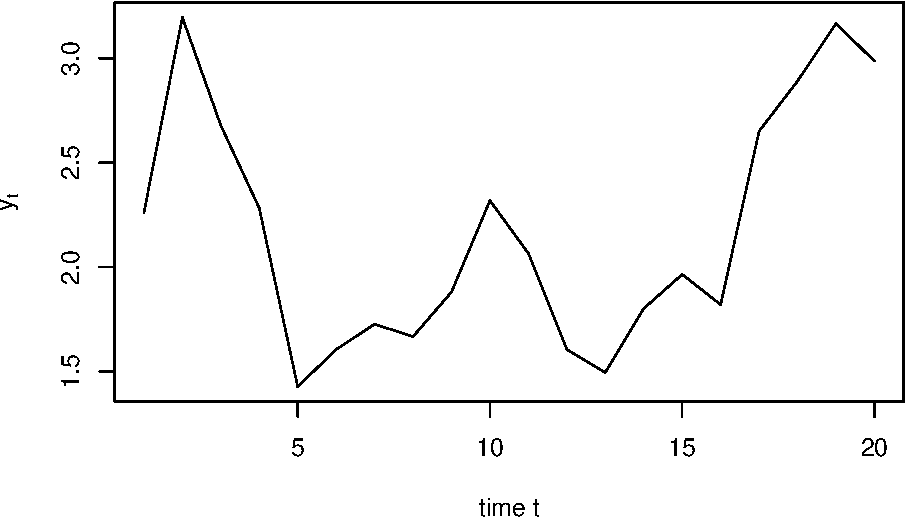
\includegraphics{EcoStat_files/figure-latex/MCMC1-1.pdf}

Next, let us write the likelihood function, i.e.~\(f_{Y|{\boldsymbol\theta}}(\mathbf{y},{\boldsymbol\theta})\). For \(\rho\), which is expected to be between 0 and 1, we use a logistic transformation. For \(\sigma\), that is expected to be positive, we use an exponential transformation.

\begin{Shaded}
\begin{Highlighting}[]
\NormalTok{likelihood }\OtherTok{\textless{}{-}} \ControlFlowTok{function}\NormalTok{(param,Y)\{}
\NormalTok{  mu  }\OtherTok{\textless{}{-}}\NormalTok{ param[}\DecValTok{1}\NormalTok{]}
\NormalTok{  rho }\OtherTok{\textless{}{-}} \FunctionTok{exp}\NormalTok{(param[}\DecValTok{2}\NormalTok{])}\SpecialCharTok{/}\NormalTok{(}\DecValTok{1}\SpecialCharTok{+}\FunctionTok{exp}\NormalTok{(param[}\DecValTok{2}\NormalTok{]))}
\NormalTok{  sigma }\OtherTok{\textless{}{-}} \FunctionTok{exp}\NormalTok{(param[}\DecValTok{3}\NormalTok{])}
\NormalTok{  MU }\OtherTok{\textless{}{-}}\NormalTok{ mu}\SpecialCharTok{/}\NormalTok{(}\DecValTok{1}\SpecialCharTok{{-}}\NormalTok{rho)}
\NormalTok{  SIGMA2 }\OtherTok{\textless{}{-}}\NormalTok{ sigma}\SpecialCharTok{\^{}}\DecValTok{2}\SpecialCharTok{/}\NormalTok{(}\DecValTok{1}\SpecialCharTok{{-}}\NormalTok{rho}\SpecialCharTok{\^{}}\DecValTok{2}\NormalTok{)}
\NormalTok{  L }\OtherTok{\textless{}{-}} \DecValTok{1}\SpecialCharTok{/}\FunctionTok{sqrt}\NormalTok{(}\DecValTok{2}\SpecialCharTok{*}\NormalTok{pi}\SpecialCharTok{*}\NormalTok{SIGMA2)}\SpecialCharTok{*}\FunctionTok{exp}\NormalTok{(}\SpecialCharTok{{-}}\NormalTok{(Y[}\DecValTok{1}\NormalTok{]}\SpecialCharTok{{-}}\NormalTok{MU)}\SpecialCharTok{\^{}}\DecValTok{2}\SpecialCharTok{/}\NormalTok{(}\DecValTok{2}\SpecialCharTok{*}\NormalTok{SIGMA2))}
\NormalTok{  Y1 }\OtherTok{\textless{}{-}}\NormalTok{ Y[}\DecValTok{2}\SpecialCharTok{:}\FunctionTok{length}\NormalTok{(Y)]}
\NormalTok{  Y0 }\OtherTok{\textless{}{-}}\NormalTok{ Y[}\DecValTok{1}\SpecialCharTok{:}\NormalTok{(}\FunctionTok{length}\NormalTok{(Y)}\SpecialCharTok{{-}}\DecValTok{1}\NormalTok{)]}
\NormalTok{  aux }\OtherTok{\textless{}{-}} \DecValTok{1}\SpecialCharTok{/}\FunctionTok{sqrt}\NormalTok{(}\DecValTok{2}\SpecialCharTok{*}\NormalTok{pi}\SpecialCharTok{*}\NormalTok{sigma}\SpecialCharTok{\^{}}\DecValTok{2}\NormalTok{)}\SpecialCharTok{*}\FunctionTok{exp}\NormalTok{(}\SpecialCharTok{{-}}\NormalTok{(Y1}\SpecialCharTok{{-}}\NormalTok{mu}\SpecialCharTok{{-}}\NormalTok{rho}\SpecialCharTok{*}\NormalTok{Y0)}\SpecialCharTok{\^{}}\DecValTok{2}\SpecialCharTok{/}\NormalTok{(}\DecValTok{2}\SpecialCharTok{*}\NormalTok{sigma}\SpecialCharTok{\^{}}\DecValTok{2}\NormalTok{))}
\NormalTok{  L }\OtherTok{\textless{}{-}}\NormalTok{ L }\SpecialCharTok{*} \FunctionTok{prod}\NormalTok{(aux)}
  \FunctionTok{return}\NormalTok{(L)}
\NormalTok{\}}
\end{Highlighting}
\end{Shaded}

Next define function \texttt{rQ} that draws from the (Gaussian) proposal distribution, as well as function \texttt{Q}, that computes \(Q_{\tilde{\boldsymbol\theta}|{\boldsymbol\theta}}(\tilde{\boldsymbol\theta},{\boldsymbol\theta})\):

\begin{Shaded}
\begin{Highlighting}[]
\NormalTok{rQ }\OtherTok{\textless{}{-}} \ControlFlowTok{function}\NormalTok{(x,a)\{}
\NormalTok{  n }\OtherTok{\textless{}{-}} \FunctionTok{length}\NormalTok{(x)}
\NormalTok{  y }\OtherTok{\textless{}{-}}\NormalTok{ x }\SpecialCharTok{+}\NormalTok{ a }\SpecialCharTok{*} \FunctionTok{rnorm}\NormalTok{(n)}
  \FunctionTok{return}\NormalTok{(y)\}}
\NormalTok{Q }\OtherTok{\textless{}{-}} \ControlFlowTok{function}\NormalTok{(y,x,a)\{}
\NormalTok{  q }\OtherTok{\textless{}{-}} \DecValTok{1}\SpecialCharTok{/}\FunctionTok{sqrt}\NormalTok{(}\DecValTok{2}\SpecialCharTok{*}\NormalTok{pi}\SpecialCharTok{*}\NormalTok{a}\SpecialCharTok{\^{}}\DecValTok{2}\NormalTok{)}\SpecialCharTok{*}\FunctionTok{exp}\NormalTok{(}\SpecialCharTok{{-}}\NormalTok{(y }\SpecialCharTok{{-}}\NormalTok{ x)}\SpecialCharTok{\^{}}\DecValTok{2}\SpecialCharTok{/}\NormalTok{(}\DecValTok{2}\SpecialCharTok{*}\NormalTok{a}\SpecialCharTok{\^{}}\DecValTok{2}\NormalTok{))}
  \FunctionTok{return}\NormalTok{(}\FunctionTok{prod}\NormalTok{(q))\}}
\end{Highlighting}
\end{Shaded}

We consider Gaussian priors:

\begin{Shaded}
\begin{Highlighting}[]
\NormalTok{prior }\OtherTok{\textless{}{-}} \ControlFlowTok{function}\NormalTok{(param,means\_prior,stdv\_prior)\{}
\NormalTok{  f }\OtherTok{\textless{}{-}} \DecValTok{1}\SpecialCharTok{/}\FunctionTok{sqrt}\NormalTok{(}\DecValTok{2}\SpecialCharTok{*}\NormalTok{pi}\SpecialCharTok{*}\NormalTok{stdv\_prior}\SpecialCharTok{\^{}}\DecValTok{2}\NormalTok{)}\SpecialCharTok{*}\FunctionTok{exp}\NormalTok{(}\SpecialCharTok{{-}}\NormalTok{(param }\SpecialCharTok{{-}} 
\NormalTok{                                         means\_prior)}\SpecialCharTok{\^{}}\DecValTok{2}\SpecialCharTok{/}\NormalTok{(}\DecValTok{2}\SpecialCharTok{*}\NormalTok{stdv\_prior}\SpecialCharTok{\^{}}\DecValTok{2}\NormalTok{))}
  \FunctionTok{return}\NormalTok{(}\FunctionTok{prod}\NormalTok{(f))\}}
\end{Highlighting}
\end{Shaded}

Function \texttt{p\_tilde} corresponds to \(f_{{\boldsymbol\theta},Y}\):

\begin{Shaded}
\begin{Highlighting}[]
\NormalTok{p\_tilde }\OtherTok{\textless{}{-}} \ControlFlowTok{function}\NormalTok{(param,Y,means\_prior,stdv\_prior)\{}
\NormalTok{  p }\OtherTok{\textless{}{-}} \FunctionTok{likelihood}\NormalTok{(param,Y) }\SpecialCharTok{*} \FunctionTok{prior}\NormalTok{(param,means\_prior,stdv\_prior)}
  \FunctionTok{return}\NormalTok{(p)\}}
\end{Highlighting}
\end{Shaded}

We can now define function \(\alpha\) (Eq. \eqref{eq:alphaXXX}):

\begin{Shaded}
\begin{Highlighting}[]
\NormalTok{alpha }\OtherTok{\textless{}{-}} \ControlFlowTok{function}\NormalTok{(y,x,means\_prior,stdv\_prior,a)\{}
\NormalTok{  aux }\OtherTok{\textless{}{-}} \FunctionTok{p\_tilde}\NormalTok{(y,Y,means\_prior,stdv\_prior)}\SpecialCharTok{/}
    \FunctionTok{p\_tilde}\NormalTok{(x,Y,means\_prior,stdv\_prior) }\SpecialCharTok{*} \FunctionTok{Q}\NormalTok{(y,x,a)}\SpecialCharTok{/}\FunctionTok{Q}\NormalTok{(x,y,a)}
\NormalTok{  alpha\_proba }\OtherTok{\textless{}{-}} \FunctionTok{min}\NormalTok{(aux,}\DecValTok{1}\NormalTok{)}
  \FunctionTok{return}\NormalTok{(alpha\_proba)\}}
\end{Highlighting}
\end{Shaded}

Now, all is set for us to write the MCMC function:

\begin{Shaded}
\begin{Highlighting}[]
\NormalTok{MCMC }\OtherTok{\textless{}{-}} \ControlFlowTok{function}\NormalTok{(Y,means\_prior,stdv\_prior,a,N)\{}
\NormalTok{  x }\OtherTok{\textless{}{-}}\NormalTok{ means\_prior}
\NormalTok{  all\_theta }\OtherTok{\textless{}{-}} \ConstantTok{NULL}
\NormalTok{  count\_accept }\OtherTok{\textless{}{-}} \DecValTok{0}
  \ControlFlowTok{for}\NormalTok{(i }\ControlFlowTok{in} \DecValTok{1}\SpecialCharTok{:}\NormalTok{N)\{}
\NormalTok{    y }\OtherTok{\textless{}{-}} \FunctionTok{rQ}\NormalTok{(x,a)}
\NormalTok{    alph }\OtherTok{\textless{}{-}} \FunctionTok{alpha}\NormalTok{(y,x,means\_prior,stdv\_prior,a)}
    \CommentTok{\#print(alph)}
\NormalTok{    u }\OtherTok{\textless{}{-}} \FunctionTok{runif}\NormalTok{(}\DecValTok{1}\NormalTok{)}
    \ControlFlowTok{if}\NormalTok{(u }\SpecialCharTok{\textless{}}\NormalTok{ alph)\{}
\NormalTok{      count\_accept }\OtherTok{\textless{}{-}}\NormalTok{ count\_accept }\SpecialCharTok{+} \DecValTok{1}
\NormalTok{      x }\OtherTok{\textless{}{-}}\NormalTok{ y\}}
\NormalTok{    all\_theta }\OtherTok{\textless{}{-}} \FunctionTok{rbind}\NormalTok{(all\_theta,x)\}}
  \FunctionTok{print}\NormalTok{(}\FunctionTok{paste}\NormalTok{(}\StringTok{"Acceptance rate:"}\NormalTok{,}\FunctionTok{toString}\NormalTok{(}\FunctionTok{round}\NormalTok{(count\_accept}\SpecialCharTok{/}\NormalTok{N,}\DecValTok{3}\NormalTok{))))}
  \FunctionTok{return}\NormalTok{(all\_theta)\}}
\end{Highlighting}
\end{Shaded}

Specify the Gaussian priors:

\begin{Shaded}
\begin{Highlighting}[]
\NormalTok{true\_values }\OtherTok{\textless{}{-}} \FunctionTok{c}\NormalTok{(mu,}\FunctionTok{log}\NormalTok{(rho}\SpecialCharTok{/}\NormalTok{(}\DecValTok{1}\SpecialCharTok{{-}}\NormalTok{rho)),}\FunctionTok{log}\NormalTok{(sigma))}
\NormalTok{means\_prior }\OtherTok{\textless{}{-}} \FunctionTok{c}\NormalTok{(}\DecValTok{1}\NormalTok{,}\DecValTok{0}\NormalTok{,}\DecValTok{0}\NormalTok{) }\CommentTok{\# as if we did not know the true values}
\NormalTok{stdv\_prior }\OtherTok{\textless{}{-}} \FunctionTok{rep}\NormalTok{(}\DecValTok{2}\NormalTok{,}\DecValTok{3}\NormalTok{)}
\NormalTok{resultMCMC }\OtherTok{\textless{}{-}} \FunctionTok{MCMC}\NormalTok{(Y,means\_prior,stdv\_prior,}\AttributeTok{a=}\NormalTok{.}\DecValTok{45}\NormalTok{,}\AttributeTok{N=}\DecValTok{20000}\NormalTok{)}
\end{Highlighting}
\end{Shaded}

\begin{verbatim}
## [1] "Acceptance rate: 0.098"
\end{verbatim}

\begin{Shaded}
\begin{Highlighting}[]
\FunctionTok{par}\NormalTok{(}\AttributeTok{mfrow=}\FunctionTok{c}\NormalTok{(}\DecValTok{2}\NormalTok{,}\DecValTok{3}\NormalTok{))}
\ControlFlowTok{for}\NormalTok{(i }\ControlFlowTok{in} \DecValTok{1}\SpecialCharTok{:}\FunctionTok{length}\NormalTok{(means\_prior))\{}
\NormalTok{  m }\OtherTok{\textless{}{-}}\NormalTok{ means\_prior[i]}
\NormalTok{  s }\OtherTok{\textless{}{-}}\NormalTok{ stdv\_prior[i]}
\NormalTok{  x }\OtherTok{\textless{}{-}} \FunctionTok{seq}\NormalTok{(m}\DecValTok{{-}3}\SpecialCharTok{*}\NormalTok{s,m}\SpecialCharTok{+}\DecValTok{3}\SpecialCharTok{*}\NormalTok{s,}\AttributeTok{length.out =} \DecValTok{100}\NormalTok{)}
  \FunctionTok{par}\NormalTok{(}\AttributeTok{mfg=}\FunctionTok{c}\NormalTok{(}\DecValTok{1}\NormalTok{,i))}
\NormalTok{  aux }\OtherTok{\textless{}{-}} \FunctionTok{density}\NormalTok{(resultMCMC[,i])}
  \FunctionTok{par}\NormalTok{(}\AttributeTok{plt=}\FunctionTok{c}\NormalTok{(.}\DecValTok{15}\NormalTok{,.}\DecValTok{95}\NormalTok{,.}\DecValTok{15}\NormalTok{,.}\DecValTok{85}\NormalTok{))}
  \FunctionTok{plot}\NormalTok{(x,}\FunctionTok{dnorm}\NormalTok{(x,m,s),}\AttributeTok{type=}\StringTok{"l"}\NormalTok{,}\AttributeTok{xlab=}\StringTok{""}\NormalTok{,}\AttributeTok{ylab=}\StringTok{""}\NormalTok{,}\AttributeTok{main=}\FunctionTok{paste}\NormalTok{(}\StringTok{"Parameter"}\NormalTok{,i),}
       \AttributeTok{ylim=}\FunctionTok{c}\NormalTok{(}\DecValTok{0}\NormalTok{,}\FunctionTok{max}\NormalTok{(aux}\SpecialCharTok{$}\NormalTok{y)))}
  \FunctionTok{lines}\NormalTok{(aux}\SpecialCharTok{$}\NormalTok{x,aux}\SpecialCharTok{$}\NormalTok{y,}\AttributeTok{col=}\StringTok{"red"}\NormalTok{,}\AttributeTok{lwd=}\DecValTok{2}\NormalTok{)}
  \FunctionTok{abline}\NormalTok{(}\AttributeTok{v=}\NormalTok{true\_values[i],}\AttributeTok{lty=}\DecValTok{2}\NormalTok{,}\AttributeTok{col=}\StringTok{"blue"}\NormalTok{)}
  \FunctionTok{par}\NormalTok{(}\AttributeTok{mfg=}\FunctionTok{c}\NormalTok{(}\DecValTok{2}\NormalTok{,i))}
  \FunctionTok{plot}\NormalTok{(resultMCMC[,i],}\DecValTok{1}\SpecialCharTok{:}\FunctionTok{length}\NormalTok{(resultMCMC[,i]),}\AttributeTok{xlim=}\FunctionTok{c}\NormalTok{(}\FunctionTok{min}\NormalTok{(x),}\FunctionTok{max}\NormalTok{(x)),}
       \AttributeTok{type=}\StringTok{"l"}\NormalTok{,}\AttributeTok{xlab=}\StringTok{""}\NormalTok{,}\AttributeTok{ylab=}\StringTok{""}\NormalTok{)\}}
\end{Highlighting}
\end{Shaded}

\begin{figure}
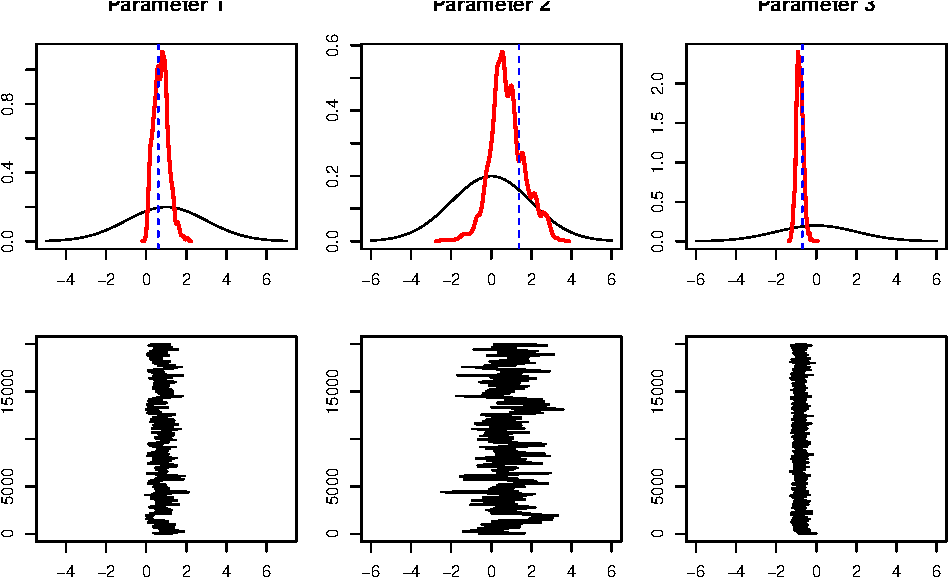
\includegraphics[width=1\linewidth]{EcoStat_files/figure-latex/MCMC8-1} \caption{The upper line of plot compares prior (black) and posterior (red) distributions. The vertical dashed blue lines indicate the true values of the parameters. The second row of plots show the sequence of $\boldsymbol\theta_i$'s generated by the MCMC algorithm. These sequences are the ones used to produce the posterior distributions (red lines) in the upper plots.}\label{fig:MCMC8}
\end{figure}

\hypertarget{binary-choice-models}{%
\chapter{Binary-choice models}\label{binary-choice-models}}

In microeconometric models, the variables of interest often feature restricted distributions ---for instance with discontinuous support---, which necessitates specific models. Typically, in many instances, the variables to be explained (the \(y_i\)'s) have only two possible values (\(0\) and \(1\), say). That is, they are binary variables. The probability for them to be equal to either 0 or 1 may depend on independent variables, gathered in vectors \(\mathbf{x}_i\) (\(K \times 1\)).

The spectrum of applications is wide:

\begin{itemize}
\tightlist
\item
  Binary decisions (e.g.~in referendums, being owner or renter, living in the city or in the countryside, in/out of the labour force,\ldots),
\item
  Contamination (disease or default),
\item
  Success/failure (exams).
\end{itemize}

Without loss of generality, the model reads:
\begin{equation}\label{eq:binaryBenroulli}
y_i | \mathbf{X} \sim \mathcal{B}(g(\mathbf{x}_i;\boldsymbol\theta)),
\end{equation}
where \(g(\mathbf{x}_i;\boldsymbol\theta)\) is the parameter of the Bernoulli distribution. In other words, conditionally on \(\mathbf{X}\):
\begin{equation}
y_i = \left\{
\begin{array}{cl}
1 & \mbox{ with probability } g(\mathbf{x}_i;\boldsymbol\theta)\\
0 & \mbox{ with probability } 1-g(\mathbf{x}_i;\boldsymbol\theta),
\end{array}
\right.\label{eq:genericBinary}
\end{equation}
where \(\boldsymbol\theta\) is a vector of parameters to be estimated.

An estimation strategy is to assume that \(g(\mathbf{x}_i;\boldsymbol\theta)\) can be proxied by \(\tilde{\boldsymbol\theta}'\mathbf{x}_i\) and to run a linear regression to estimate \(\tilde{\boldsymbol\theta}\) (a situation called \textbf{Linear Probability Model, LPM}):
\[
y_i = \tilde{\boldsymbol\theta}'\mathbf{x}_i + \varepsilon_i.
\]
Notwithstanding the fact that this specification does not exclude negative probabilities or probabilities greater than one, it could be compatible with the \emph{assumption of zero conditional mean} (Hypothesis \ref{hyp:exogeneity}) and with the \emph{assumption of non-correlated residuals} (Hypothesis \ref{hyp:noncorrelResid}), but more difficultly with the \emph{homoskedasticity assumption} (Hypothesis \ref{hyp:homoskedasticity}). Moreover, the \(\varepsilon_i\)'s cannot be Gaussian (because \(y_i \in \{0,1\}\)). Hence, using a linear regression to study the relationship between \(\mathbf{x}_i\) and \(y_i\) can be consistent but it is inefficient.

Figure \ref{fig:LPM} illustrates the fit resulting from an application of the LPM model to binary (dependent) variables.

\begin{figure}
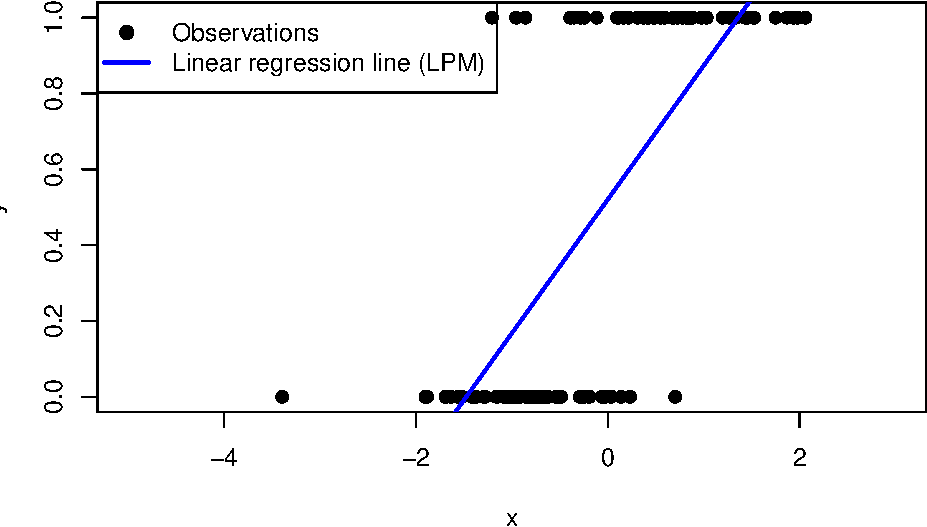
\includegraphics[width=0.95\linewidth]{EcoStat_files/figure-latex/LPM-1} \caption{Fitting a binary variable with a linear model (Linear Probability Model, LPM). The model is $\mathbb{P}(y_i=1|x_i)=\Phi(0.5+2x_i)$, where $\Phi$ is the c.d.f. of the normal distribution and where $x_i \sim \,i.i.d.\,\mathcal{N}(0,1)$.}\label{fig:LPM}
\end{figure}

Except for its last row (LPM case), Table \ref{tab:foo} provides examples of functions \(g\) valued in \([0,1]\), and that can therefore used in models of the type: \(\mathbb{P}(y_i=1|\mathbf{x}_i;\boldsymbol\theta) = g(\boldsymbol\theta'\mathbf{x}_i)\) (see Eq. \eqref{eq:genericBinary}). The ``linear'' case is given for comparison, but note that it does not satisfy \(g(\boldsymbol\theta'\mathbf{x}_i) \in [0,1]\) for any value of \(\boldsymbol\theta'\mathbf{x}_i\).

\begin{longtable}[]{@{}
  >{\raggedright\arraybackslash}p{(\columnwidth - 4\tabcolsep) * \real{0.2143}}
  >{\raggedright\arraybackslash}p{(\columnwidth - 4\tabcolsep) * \real{0.3571}}
  >{\raggedright\arraybackslash}p{(\columnwidth - 4\tabcolsep) * \real{0.4286}}@{}}
\caption{\label{tab:foo} This table provides examples of function \(g\), s.t. \(\mathbb{P}(y_i=1|\mathbf{x}_i;\boldsymbol heta) = g(\boldsymbol\theta'\mathbf{x}_i)\). The LPM case (last row) is given for comparison but, again, it does not satisfy \(g(\boldsymbol\theta'\mathbf{x}_i) \in [0,1]\) for any value of \(\boldsymbol\theta'\mathbf{x}_i\).}\tabularnewline
\toprule()
\begin{minipage}[b]{\linewidth}\raggedright
Model
\end{minipage} & \begin{minipage}[b]{\linewidth}\raggedright
Function \(g\)
\end{minipage} & \begin{minipage}[b]{\linewidth}\raggedright
Derivative
\end{minipage} \\
\midrule()
\endfirsthead
\toprule()
\begin{minipage}[b]{\linewidth}\raggedright
Model
\end{minipage} & \begin{minipage}[b]{\linewidth}\raggedright
Function \(g\)
\end{minipage} & \begin{minipage}[b]{\linewidth}\raggedright
Derivative
\end{minipage} \\
\midrule()
\endhead
Probit & \(\Phi\) & \(\phi\) \\
Logit & \(\dfrac{\exp(x)}{1+\exp(x)}\) & \(\dfrac{\exp(x)}{(1+\exp(x))^2}\) \\
log-log & \(1 - \exp(-\exp(x))\) & \(\exp(-\exp(x))\exp(x)\) \\
linear (LPM) & \(x\) & 1 \\
\bottomrule()
\end{longtable}

Figure \ref{fig:ProbLogit} displays the first three \(g\) functions appearing in Table \ref{tab:foo}.

\begin{figure}
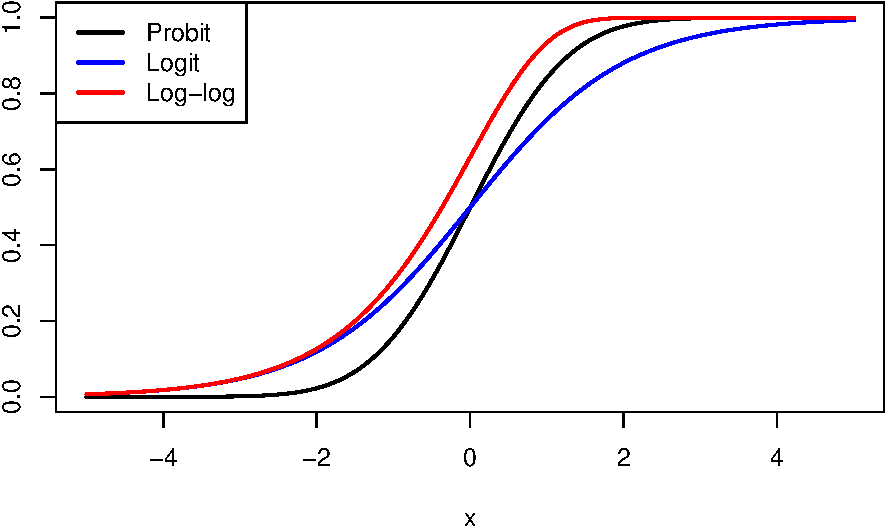
\includegraphics[width=0.95\linewidth]{EcoStat_files/figure-latex/ProbLogit-1} \caption{Probit, Logit, and Log-log functions.}\label{fig:ProbLogit}
\end{figure}

The \textbf{probit} and the \textbf{logit} models are popular binary-choice models. In the probit model, we have:
\begin{equation}
g(z) = \Phi(z),\label{eq:probit}
\end{equation}
where \(\Phi\) is the c.d.f. of the normal distribution. And for the logit model:
\begin{equation}
g(z) = \frac{1}{1+\exp(-z)}.\label{eq:logit}
\end{equation}

Figure \ref{fig:LPM2} shows the conditional probabilities associated with the (probit) model that had been used to generate the data of Figure \ref{fig:LPM}.

\begin{figure}
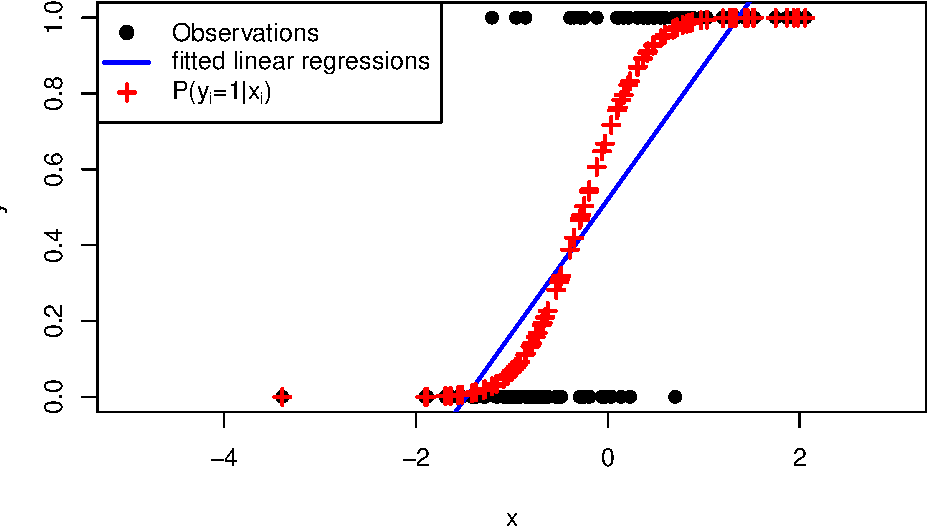
\includegraphics[width=0.95\linewidth]{EcoStat_files/figure-latex/LPM2-1} \caption{The model is $\mathbb{P}(y_i=1|x_i)=\Phi(0.5+2x_i)$, where $\Phi$ is the c.d.f. of the normal distribution and where $x_i \sim \,i.i.d.\,\mathcal{N}(0,1)$. Crosses give the model-implied probabilities of having $y_i=1$ (conditional on $x_i$).}\label{fig:LPM2}
\end{figure}

\hypertarget{latent}{%
\section{Interpretation in terms of latent variable, and utility-based models}\label{latent}}

The probit model has an interpretation in terms of latent variables, which, in turn, is often exploited in structural models, called \textbf{Random Utility Models (RUM)}. In such structural models, it is assumed that the agents that have to take the decision do so by selecting the outcome that provides them with the larger utility (for agent \(i\), two possible outcomes: \(y_i=0\) or \(y_i=1\)). Part of this utility is observed by the econometrician ---it depends on the covariates \(\mathbf{x}_i\)--- and part of it is latent.

In the probit model, we have:
\[
\mathbb{P}(y_i=1|\mathbf{x}_i;\boldsymbol\theta) = \Phi(\boldsymbol\theta'\mathbf{x}_i) = \mathbb{P}(-\varepsilon_{i}<\boldsymbol\theta'\mathbf{x}_i),
\]
where \(\varepsilon_{i} \sim \mathcal{N}(0,1)\). That is:
\[
\mathbb{P}(y_i=1|\mathbf{x}_i;\boldsymbol\theta) = \mathbb{P}(0< y_i^*),
\]
where \(y_i^* = \boldsymbol\theta'\mathbf{x}_i + \varepsilon_i\), with \(\varepsilon_{i} \sim \mathcal{N}(0,1)\). Variable \(y_i^*\) can be interpreted as a (latent) variable that determines \(y_i\) (since \(y_i = \mathbb{I}_{\{y_i^*>0\}}\)).

Figure \ref{fig:Latent} illustrates this situation.

\begin{figure}
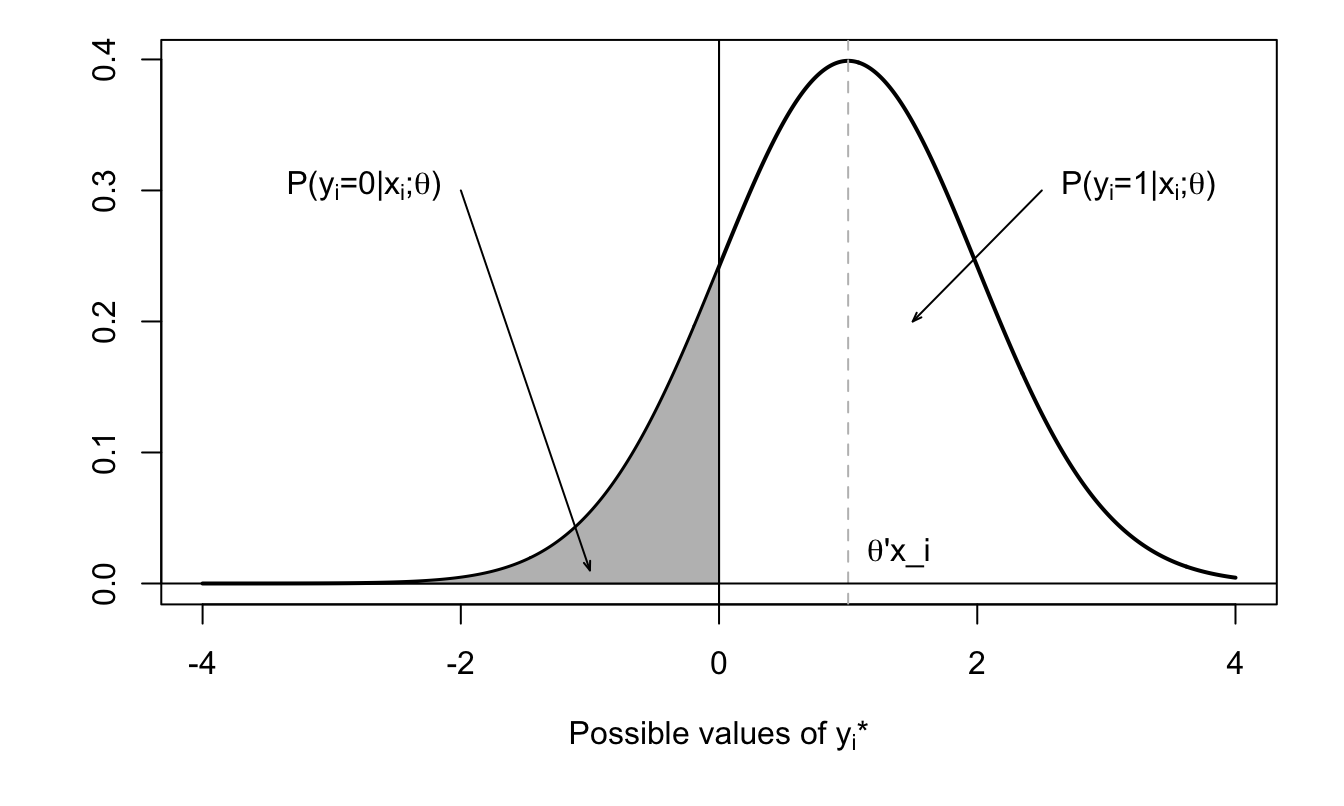
\includegraphics[width=0.95\linewidth]{EcoStat_files/figure-latex/Latent-1} \caption{Distribution of $y_i^*$ conditional on $\mathbf{x}_i$.}\label{fig:Latent}
\end{figure}

Assume that agent (\(i\)) chooses \(y_i=1\) if the utility associated with this choice (\(U_{i,1}\)) is higher than the one associated with \(y_i=0\) (that is \(U_{i,0}\)). Assume further that the utility of agent \(i\), if she chooses outcome \(j\) (\(\in \{0,1\}\)), is given by
\[
U_{i,j} = V_{i,j} + \varepsilon_{i,j},
\]
where \(V_{i,j}\) is the deterministic component of the utility associated with choice and where \(\varepsilon_{i,j}\) is a random (agent-specific) component. Moreover, posit \(V_{i,j} = \boldsymbol\theta_j'\mathbf{x}_i\). We then have:
\begin{eqnarray}
\mathbb{P}(y_i = 1|\mathbf{x}_i;\boldsymbol\theta) &=& \mathbb{P}(\boldsymbol\theta_1'\mathbf{x}_i+\varepsilon_{i,1}>\boldsymbol\theta_0'\mathbf{x}_i+\varepsilon_{i,0}) \nonumber\\
&=& F(\boldsymbol\theta_1'\mathbf{x}_i-\boldsymbol\theta_0'\mathbf{x}_i) = F([\boldsymbol\theta_1-\boldsymbol\theta_0]'\mathbf{x}_i),\label{eq:utility}
\end{eqnarray}
where \(F\) is the c.d.f. of \(\varepsilon_{i,0}-\varepsilon_{i,1}\).

Note that only the difference \(\boldsymbol\theta_1-\boldsymbol\theta_0\) is identifiable (as opposed to \(\boldsymbol\theta_1\) \emph{and} \(\boldsymbol\theta_0\)). Indeed, replacing \(U\) with \(aU\) (\(a>0\)) gives the same model. This \emph{scaling} issue can be solved by fixing the variance of \(\varepsilon_{i,0}-\varepsilon_{i,1}\).

\begin{example}[Migration and income]
\protect\hypertarget{exm:migration}{}\label{exm:migration}The RUM approach has been used by \citet{Nakosteen_Zimmer_1980} to study migration choices. Their model is based on the comparison of marginal costs and benefits associated with migration. The main ingredients of their approach are as follows:

\begin{itemize}
\tightlist
\item
  Wage that can be earned at the present location: \(y_p^* = \boldsymbol\theta_p'\mathbf{x}_p + \varepsilon_p\).
\item
  Migration cost: \(C^*= \boldsymbol\theta_c'\mathbf{x}_c + \varepsilon_c\).
\item
  Wage earned elsewhere: \(y_m^* = \boldsymbol\theta_m'\mathbf{x}_m + \varepsilon_m\).
\end{itemize}

In this context, agents decision to migrate if \(y_m^* > y_p^* + C^*\), i.e.~if
\[
y^* = y_m^* -  y_p^* - C^* =  \boldsymbol\theta'\mathbf{x} + \underbrace{\varepsilon}_{=\varepsilon_m - \varepsilon_c - \varepsilon_p}>0,
\]
where \(\mathbf{x}\) is the union of the \(\mathbf{x}_i\)s, for \(i \in \{p,m,c\}\).
\end{example}

\hypertarget{Avregressors}{%
\section{Alternative-Varying Regressors}\label{Avregressors}}

In some cases, regressors may depend on the considered alternative (\(0\) or \(1\)). For instance:

\begin{itemize}
\tightlist
\item
  When modeling the decision to participate in the labour force (or not), the wage depends on the alternative. Typically, it is zero if the considered agent has decided not to work (and strictly positive otherwise).
\item
  In the context of the choice of transportation mode, ``time cost'' depends on the considered transportation mode.
\end{itemize}

In terms of utility, we then have:
\[
V_{i,j} = {\theta^{(u)}_{j}}'\mathbf{u}_{i,j} + {\theta^{(v)}_{j}}'\mathbf{v}_{i},
\]
where the \(\mathbf{u}_{i,j}\)'s are regressors associated with agent \(i\), but taking different values for the different choices (\(j=0\) or \(j=1\)). In that case, Eq. \eqref{eq:utility} becomes:
\begin{equation}
\mathbb{P}(y_i = 1|\mathbf{x}_i;\boldsymbol\theta)  = F\left({\theta^{(u)}_{1}}'\mathbf{u}_{i,1}-{\theta^{(u)}_{0}}'\mathbf{u}_{i,0}+[\boldsymbol\theta_1^{(v)}-\boldsymbol\theta_0^{(v)}]'\mathbf{v}_i\right),\label{eq:utility2}
\end{equation}
and, if \(\theta^{(u)}_{1}=\theta^{(u)}_{0}=\theta^{(u)}\) ---as is customary--- we get:
\begin{equation}
\mathbb{P}(y_i = 1|\mathbf{x}_i;\boldsymbol\theta)  = F\left({\theta^{(u)}_{1}}'(\mathbf{u}_{i,1}-\mathbf{u}_{i,0})+[\boldsymbol\theta_1^{(v)}-\boldsymbol\theta_0^{(v)}]'\mathbf{v}_i\right).\label{eq:utility3}
\end{equation}

\begin{example}[Fishing-mode dataset]
\protect\hypertarget{exm:FishingTable}{}\label{exm:FishingTable}

The fishing-mode dataset used in \citet{Cameron_Trivedi_2005} (Chapters 14 and 15) contains alternative-specific variables. Specifically, for each individual, the price and catch rate depend on the fishing model. In the table reported below, lines \texttt{price} and \texttt{catch} correspond to the prices and catch rates associated with the chosen alternative.

\begin{Shaded}
\begin{Highlighting}[]
\FunctionTok{library}\NormalTok{(mlogit)}
\FunctionTok{data}\NormalTok{(}\StringTok{"Fishing"}\NormalTok{,}\AttributeTok{package=}\StringTok{"mlogit"}\NormalTok{)}
\NormalTok{stargazer}\SpecialCharTok{::}\FunctionTok{stargazer}\NormalTok{(Fishing,}\AttributeTok{type=}\StringTok{"text"}\NormalTok{)}
\end{Highlighting}
\end{Shaded}

\begin{verbatim}
## 
## ==========================================================
## Statistic       N     Mean    St. Dev.    Min      Max    
## ----------------------------------------------------------
## price.beach   1,182  103.422   103.641   1.290   843.186  
## price.pier    1,182  103.422   103.641   1.290   843.186  
## price.boat    1,182  55.257    62.713    2.290   666.110  
## price.charter 1,182  84.379    63.545   27.290   691.110  
## catch.beach   1,182   0.241     0.191    0.068    0.533   
## catch.pier    1,182   0.162     0.160    0.001    0.452   
## catch.boat    1,182   0.171     0.210   0.0002    0.737   
## catch.charter 1,182   0.629     0.706    0.002    2.310   
## income        1,182 4,099.337 2,461.964 416.667 12,500.000
## ----------------------------------------------------------
\end{verbatim}

\end{example}

\hypertarget{estimation}{%
\section{Estimation}\label{estimation}}

These models can be estimated by Maximum Likelihood approaches (see Section \ref{secMLE}).

To simplify the exposition, we consider the \(\mathbf{x}_i\) vectors of covariates to be deterministic. Moreover, we assume that the r.v. are independent across entities \(i\). How to write the likelihood in that case? It is easily checked that:
\[
f(y_i|\mathbf{x}_i;\boldsymbol\theta) =   g(\boldsymbol\theta'\mathbf{x}_i)^{y_i}(1-g(\boldsymbol\theta'\mathbf{x}_i))^{1-y_i}.
\]

Therefore, if the observations \((\mathbf{x}_i,y_i)\) are independent across entities \(i\), we obtain:
\[
\log \mathcal{L}(\boldsymbol\theta;\mathbf{y},\mathbf{X}) = \sum_{i=1}^{n}y_i \log[g(\boldsymbol\theta'\mathbf{x}_i)] + (1-y_i)\log[1-g(\boldsymbol\theta'\mathbf{x}_i)].
\]

The likelihood equation reads (FOC of the optimization program, see Def. \ref{def:likFunction}):
\[
\dfrac{\partial \log \mathcal{L}(\boldsymbol\theta;\mathbf{y},\mathbf{X})}{\partial \boldsymbol\theta} = \mathbf{0},
\]
that is:
\[
\sum_{i=1}^{n} y_i \mathbf{x}_i\frac{g'(\boldsymbol\theta'\mathbf{x}_i)}{g(\boldsymbol\theta'\mathbf{x}_i)} - (1-y_i) \mathbf{x}_i \frac{g'(\boldsymbol\theta'\mathbf{x}_i)}{1-g(\boldsymbol\theta'\mathbf{x}_i)} = \mathbf{0}.
\]

This is a nonlinear (multivariate) equation that can be solved numerically. Under regularity conditions (Hypotheses \ref{hyp:MLEregularity}), we approximately have (Prop. \ref{prp:MLEproperties}):
\[
\boldsymbol\theta_{MLE} \sim \mathcal{N}(\boldsymbol\theta_0,\mathbf{I}(\boldsymbol\theta_0)^{-1}),
\]
where
\[
\mathbf{I}(\boldsymbol\theta_0) = - \mathbb{E}_0 \left( \frac{\partial^2 \log \mathcal{L}(\theta;\mathbf{y},\mathbf{X})}{\partial \boldsymbol\theta \partial \boldsymbol\theta'}\right) = n \mathcal{I}_Y(\boldsymbol\theta_0).
\]

For finite samples, we can e.g.~approximate \(\mathbf{I}(\boldsymbol\theta_0)^{-1}\) by Eq. \eqref{eq:III1}:
\[
\mathbf{I}(\boldsymbol\theta_0)^{-1} \approx -\left(\frac{\partial^2 \log \mathcal{L}(\boldsymbol\theta_{MLE};\mathbf{y},\mathbf{X})}{\partial \boldsymbol\theta \partial \boldsymbol\theta'}\right)^{-1}.
\]

In the Probit case (see Table \ref{tab:foo}), it can be shown that we have:
\begin{eqnarray*}
&&\frac{\partial^2 \log \mathcal{L}(\boldsymbol\theta;\mathbf{y},\mathbf{X})}{\partial \boldsymbol\theta \partial \boldsymbol\theta'} = - \sum_{i=1}^{n} g'(\boldsymbol\theta'\mathbf{x}_i) [\mathbf{x}_i \mathbf{x}_i'] \times \\
&&\left[y_i \frac{g'(\boldsymbol\theta'\mathbf{x}_i) + \boldsymbol\theta'\mathbf{x}_ig(\boldsymbol\theta'\mathbf{x}_i)}{g(\boldsymbol\theta'\mathbf{x}_i)^2} + (1-y_i) \frac{g'(\boldsymbol\theta'\mathbf{x}_i) - \boldsymbol\theta'\mathbf{x}_i (1 - g(\boldsymbol\theta'\mathbf{x}_i))}{(1-g(\boldsymbol\theta'\mathbf{x}_i))^2}\right].
\end{eqnarray*}

In the Logit case (see Table \ref{tab:foo}), it can be shown that we have:
\[
\frac{\partial^2 \log \mathcal{L}(\boldsymbol\theta;\mathbf{y},\mathbf{X})}{\partial \boldsymbol\theta \partial \boldsymbol\theta'} = - \sum_{i=1}^{n} g'(\boldsymbol\theta'\mathbf{x}_i) \mathbf{x}_i\mathbf{x}_i',
\]
where \(g'(x)=\dfrac{\exp(-x)}{(1 + \exp(-x))^2}\).

Remark that, since \(g'(x)>0\), \(-\partial^2 \log \mathcal{L}(\boldsymbol\theta;\mathbf{y},\mathbf{X})/\partial \boldsymbol\theta \partial \boldsymbol\theta'\) is positive definite.

\hypertarget{marginalFX}{%
\section{Marginal effects}\label{marginalFX}}

How to measure marginal effects, i.e.~the effect on the probability that \(y_i=1\) of a marginal increase of \(x_{i,k}\)? This object is given by:
\[
\frac{\partial \mathbb{P}(y_i=1|\mathbf{x}_i;\boldsymbol\theta)}{\partial x_{i,k}} = \underbrace{g'(\boldsymbol\theta'\mathbf{x}_i)}_{>0}\theta_k,
\]
which is of the same sign as \(\theta_k\) if function \(g\) is monotonously increasing.

For agent \(i\), this marginal effect is consistently estimated by \(g'(\boldsymbol\theta_{MLE}'\mathbf{x}_i)\theta_{MLE,k}\). It is important to see that the marginal effect depends on \(\mathbf{x}_i\): respective increases by 1 unit of \(x_{i,k}\) (entity \(i\)) and of \(x_{j,k}\) (entity \(j\)) do not necessarily have the same effect on \(\mathbb{P}(y_i=1|\mathbf{x}_i;\boldsymbol\theta)\) as on \(\mathbb{P}(y_j=1|\mathbf{x}_j;\boldsymbol\theta)\). To address this issue, one can compute some measures of ``average'' marginal effect. There are two main solutions. For each explanatory variable \(k\):

\begin{enumerate}
\def\labelenumi{\roman{enumi}.}
\tightlist
\item
  Denoting by \(\hat{\mathbf{x}}\) the sample average of the \(\mathbf{x}_i\)s, compute \(g'(\boldsymbol\theta_{MLE}'\hat{\mathbf{x}})\theta_{MLE,k}\).
\item
  Compute the average (across \(i\)) of \(g'(\boldsymbol\theta_{MLE}'\mathbf{x}_i)\theta_{MLE,k}\).
\end{enumerate}

\hypertarget{goodness-of-fit-1}{%
\section{Goodness of fit}\label{goodness-of-fit-1}}

There is no obvious version of ``\(R^2\)'' for binary-choice models. Existing measures are called \textbf{pseudo-\(R^2\) measures}.

Denoting by \(\log \mathcal{L}_0(\mathbf{y})\) the (maximum) log-likelihood that would be obtained for a model containing only a constant term (i.e.~with \(\mathbf{x}_i = 1\) for all \(i\)), the McFadden's pseudo-\(R^2\) is given by:
\[
R^2_{MF} = 1 - \frac{\log \mathcal{L}(\boldsymbol\theta;\mathbf{y})}{\log \mathcal{L}_0(\mathbf{y})}.
\]
Intuitively, \(R^2_{MF}=0\) if the explanatory variables do not convey any information on the outcome \(y\). Indeed, in this case, the model is not better than the reference model, that simply captures the fraction of \(y_i\)'s that are equal to 1.

\begin{example}[Credit and defaults (Lending-club dataset)]
\protect\hypertarget{exm:creditProbit}{}\label{exm:creditProbit}This example makes use of the \texttt{credit} data of package \texttt{AEC}. The objective is to model the default probabilities of borrowers.

Let us first represent the relationship between the fraction of households that have defaulted on their loan and their annual income:

\begin{Shaded}
\begin{Highlighting}[]
\FunctionTok{library}\NormalTok{(AEC)}
\NormalTok{credit}\SpecialCharTok{$}\NormalTok{Default }\OtherTok{\textless{}{-}} \DecValTok{0}
\NormalTok{credit}\SpecialCharTok{$}\NormalTok{Default[credit}\SpecialCharTok{$}\NormalTok{loan\_status }\SpecialCharTok{==} \StringTok{"Charged Off"}\NormalTok{] }\OtherTok{\textless{}{-}} \DecValTok{1}
\NormalTok{credit}\SpecialCharTok{$}\NormalTok{Default[credit}\SpecialCharTok{$}\NormalTok{loan\_status }\SpecialCharTok{==}
                 \StringTok{"Does not meet the credit policy. Status:Charged Off"}\NormalTok{] }\OtherTok{\textless{}{-}} \DecValTok{1}
\NormalTok{credit}\SpecialCharTok{$}\NormalTok{amt2income }\OtherTok{\textless{}{-}}\NormalTok{ credit}\SpecialCharTok{$}\NormalTok{loan\_amnt}\SpecialCharTok{/}\NormalTok{credit}\SpecialCharTok{$}\NormalTok{annual\_inc}
\FunctionTok{plot}\NormalTok{(}\FunctionTok{as.factor}\NormalTok{(credit}\SpecialCharTok{$}\NormalTok{Default)}\SpecialCharTok{\textasciitilde{}}\FunctionTok{log}\NormalTok{(credit}\SpecialCharTok{$}\NormalTok{annual\_inc),}
     \AttributeTok{ylevels=}\DecValTok{2}\SpecialCharTok{:}\DecValTok{1}\NormalTok{,}\AttributeTok{ylab=}\StringTok{"Default status"}\NormalTok{,}\AttributeTok{xlab=}\StringTok{"log(annual income)"}\NormalTok{)}
\end{Highlighting}
\end{Shaded}

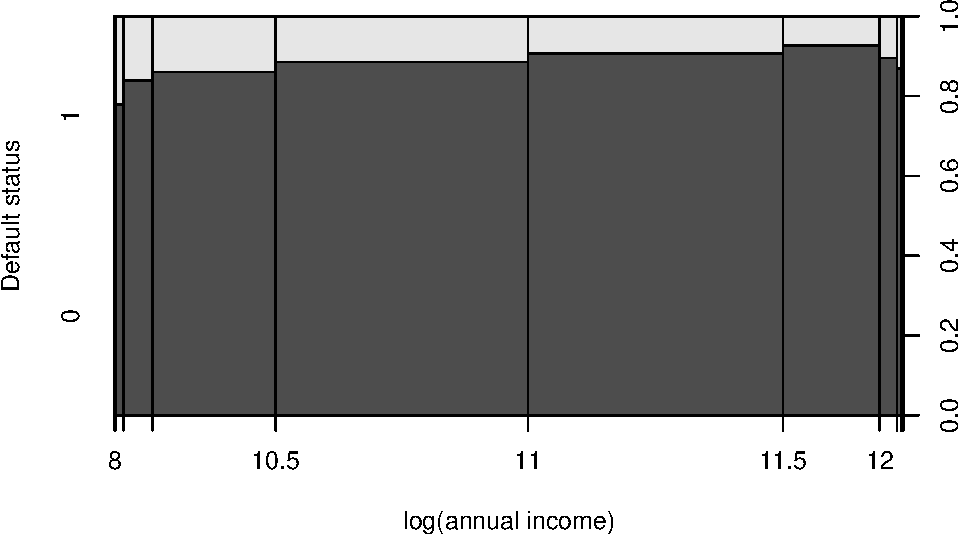
\includegraphics{EcoStat_files/figure-latex/Probitlending-1.pdf}

The previous figure suggests that the effect of annual income on the probability of default is non-monotonous. We will therefore include a quadratic term in one of our specification (namely \texttt{eq1} below).

We consider three specifications. The first one (\texttt{eq0}), with no explanatory variables, is trivial. It will just be used to compute the pseudo-\(R^2\). In the second (\texttt{eq1}), we consider a few covariates (loan amount, the ratio between the amount and annual income, The number of more-than-30 days past-due incidences of delinquency in the borrower's credit file for the past 2 years, and a quadratic function of annual income). In the third model (\texttt{eq2}), we add a credit rating.

\begin{Shaded}
\begin{Highlighting}[]
\NormalTok{eq0 }\OtherTok{\textless{}{-}} \FunctionTok{glm}\NormalTok{(Default }\SpecialCharTok{\textasciitilde{}} \DecValTok{1}\NormalTok{,}\AttributeTok{data=}\NormalTok{credit,}\AttributeTok{family=}\FunctionTok{binomial}\NormalTok{(}\AttributeTok{link=}\StringTok{"probit"}\NormalTok{))}
\NormalTok{eq1 }\OtherTok{\textless{}{-}} \FunctionTok{glm}\NormalTok{(Default }\SpecialCharTok{\textasciitilde{}} \FunctionTok{log}\NormalTok{(loan\_amnt) }\SpecialCharTok{+}\NormalTok{ amt2income }\SpecialCharTok{+}\NormalTok{ delinq\_2yrs }\SpecialCharTok{+} 
             \FunctionTok{log}\NormalTok{(annual\_inc)}\SpecialCharTok{+} \FunctionTok{I}\NormalTok{(}\FunctionTok{log}\NormalTok{(annual\_inc)}\SpecialCharTok{\^{}}\DecValTok{2}\NormalTok{),}
           \AttributeTok{data=}\NormalTok{credit,}\AttributeTok{family=}\FunctionTok{binomial}\NormalTok{(}\AttributeTok{link=}\StringTok{"probit"}\NormalTok{))}
\NormalTok{eq2 }\OtherTok{\textless{}{-}} \FunctionTok{glm}\NormalTok{(Default }\SpecialCharTok{\textasciitilde{}}\NormalTok{ grade }\SpecialCharTok{+} \FunctionTok{log}\NormalTok{(loan\_amnt) }\SpecialCharTok{+}\NormalTok{ amt2income }\SpecialCharTok{+}\NormalTok{ delinq\_2yrs }\SpecialCharTok{+} 
             \FunctionTok{log}\NormalTok{(annual\_inc)}\SpecialCharTok{+} \FunctionTok{I}\NormalTok{(}\FunctionTok{log}\NormalTok{(annual\_inc)}\SpecialCharTok{\^{}}\DecValTok{2}\NormalTok{),}
           \AttributeTok{data=}\NormalTok{credit,}\AttributeTok{family=}\FunctionTok{binomial}\NormalTok{(}\AttributeTok{link=}\StringTok{"probit"}\NormalTok{))}
\NormalTok{stargazer}\SpecialCharTok{::}\FunctionTok{stargazer}\NormalTok{(eq0,eq1,eq2,}\AttributeTok{type=}\StringTok{"text"}\NormalTok{,}\AttributeTok{no.space =} \ConstantTok{TRUE}\NormalTok{)}
\end{Highlighting}
\end{Shaded}

\begin{verbatim}
## 
## ====================================================
##                           Dependent variable:       
##                     --------------------------------
##                                 Default             
##                        (1)        (2)        (3)    
## ----------------------------------------------------
## gradeB                                     0.400*** 
##                                            (0.055)  
## gradeC                                     0.587*** 
##                                            (0.057)  
## gradeD                                     0.820*** 
##                                            (0.061)  
## gradeE                                     0.874*** 
##                                            (0.091)  
## gradeF                                     1.230*** 
##                                            (0.147)  
## gradeG                                     1.439*** 
##                                            (0.227)  
## log(loan_amnt)                  -0.149**  -0.194*** 
##                                 (0.060)    (0.061)  
## amt2income                      1.266***   1.222*** 
##                                 (0.383)    (0.393)  
## delinq_2yrs                     0.096***    0.009   
##                                 (0.034)    (0.035)  
## log(annual_inc)                 -1.444**    -0.874  
##                                 (0.569)    (0.586)  
## I(log(annual_inc)2)             0.064**     0.038   
##                                 (0.025)    (0.026)  
## Constant            -1.231***   7.937***    4.749   
##                      (0.017)    (3.060)    (3.154)  
## ----------------------------------------------------
## Observations          9,156      9,156      9,156   
## Log Likelihood      -3,157.696 -3,120.625 -2,981.343
## Akaike Inf. Crit.   6,317.392  6,253.250  5,986.686 
## ====================================================
## Note:                    *p<0.1; **p<0.05; ***p<0.01
\end{verbatim}

Let us compute the pseudo R2 for the last two models:

\begin{Shaded}
\begin{Highlighting}[]
\NormalTok{logL0 }\OtherTok{\textless{}{-}} \FunctionTok{logLik}\NormalTok{(eq0);logL1 }\OtherTok{\textless{}{-}} \FunctionTok{logLik}\NormalTok{(eq1);logL2 }\OtherTok{\textless{}{-}} \FunctionTok{logLik}\NormalTok{(eq2)}
\NormalTok{pseudoR2\_eq1 }\OtherTok{\textless{}{-}} \DecValTok{1} \SpecialCharTok{{-}}\NormalTok{ logL1}\SpecialCharTok{/}\NormalTok{logL0 }\CommentTok{\# pseudo R2}
\NormalTok{pseudoR2\_eq2 }\OtherTok{\textless{}{-}} \DecValTok{1} \SpecialCharTok{{-}}\NormalTok{ logL2}\SpecialCharTok{/}\NormalTok{logL0 }\CommentTok{\# pseudo R2}
\FunctionTok{c}\NormalTok{(pseudoR2\_eq1,pseudoR2\_eq2)}
\end{Highlighting}
\end{Shaded}

\begin{verbatim}
## [1] 0.01173993 0.05584870
\end{verbatim}

Let us now compute the (average) marginal effects, using method ii of Section \ref{marginalFX}:

\begin{Shaded}
\begin{Highlighting}[]
\FunctionTok{mean}\NormalTok{(}\FunctionTok{dnorm}\NormalTok{(}\FunctionTok{predict}\NormalTok{(eq2)),}\AttributeTok{na.rm=}\ConstantTok{TRUE}\NormalTok{)}\SpecialCharTok{*}\NormalTok{eq2}\SpecialCharTok{$}\NormalTok{coefficients}
\end{Highlighting}
\end{Shaded}

\begin{verbatim}
##          (Intercept)               gradeB               gradeC 
##          0.840731198          0.070747353          0.103944305 
##               gradeD               gradeE               gradeF 
##          0.145089219          0.154773742          0.217702041 
##               gradeG       log(loan_amnt)           amt2income 
##          0.254722161         -0.034289921          0.216251992 
##          delinq_2yrs      log(annual_inc) I(log(annual_inc)^2) 
##          0.001574178         -0.154701321          0.006813694
\end{verbatim}

There is an issue for the \texttt{annual\_inc} variable. Indeed, the previous computation does not realize that this variable appears twice among the explanatory variables (through \texttt{log(annual\_inc)} and \texttt{I(log(annual\_inc)\^{}2)}). To address this, one can proceed as follows: (1) we construct a new counterfactual dataset where annual incomes are increased by 1\%, (2) we use the model to compute model-implied probabilities of default on this new dataset and (3), we subtract the probabilities resulting from the original dataset from these counterfactual probabilities:

\begin{Shaded}
\begin{Highlighting}[]
\NormalTok{new\_credit }\OtherTok{\textless{}{-}}\NormalTok{ credit}
\NormalTok{new\_credit}\SpecialCharTok{$}\NormalTok{annual\_inc }\OtherTok{\textless{}{-}} \FloatTok{1.01} \SpecialCharTok{*}\NormalTok{ new\_credit}\SpecialCharTok{$}\NormalTok{annual\_inc}
\NormalTok{bas\_predict\_eq2  }\OtherTok{\textless{}{-}} \FunctionTok{predict}\NormalTok{(eq2, }\AttributeTok{newdata =}\NormalTok{ credit, }\AttributeTok{type =} \StringTok{"response"}\NormalTok{)}
\CommentTok{\# This is equivalent to pnorm(predict(eq2, newdata = credit))}
\NormalTok{new\_predict\_eq2  }\OtherTok{\textless{}{-}} \FunctionTok{predict}\NormalTok{(eq2, }\AttributeTok{newdata =}\NormalTok{ new\_credit, }\AttributeTok{type =} \StringTok{"response"}\NormalTok{)}
\FunctionTok{mean}\NormalTok{(new\_predict\_eq2 }\SpecialCharTok{{-}}\NormalTok{ bas\_predict\_eq2)}
\end{Highlighting}
\end{Shaded}

\begin{verbatim}
## [1] -6.562126e-05
\end{verbatim}

The negative sign means that, on average across the entities considered in the analysis, a 1\% increase in annual income results in a decrease in the default probability. This average effect is however pretty low. To get an economic sense of the size of this effect, let us compute the average effect associated with a unit increase in the number of delinquencies:

\begin{Shaded}
\begin{Highlighting}[]
\NormalTok{new\_credit }\OtherTok{\textless{}{-}}\NormalTok{ credit}
\NormalTok{new\_credit}\SpecialCharTok{$}\NormalTok{delinq\_2yrs }\OtherTok{\textless{}{-}}\NormalTok{ credit}\SpecialCharTok{$}\NormalTok{delinq\_2yrs }\SpecialCharTok{+} \DecValTok{1}
\NormalTok{new\_predict\_eq2  }\OtherTok{\textless{}{-}} \FunctionTok{predict}\NormalTok{(eq2, }\AttributeTok{newdata =}\NormalTok{ new\_credit, }\AttributeTok{type =} \StringTok{"response"}\NormalTok{)}
\FunctionTok{mean}\NormalTok{(new\_predict\_eq2 }\SpecialCharTok{{-}}\NormalTok{ bas\_predict\_eq2)}
\end{Highlighting}
\end{Shaded}

\begin{verbatim}
## [1] 0.001582332
\end{verbatim}

We can employ a likelihood ratio test (see Def. \ref{def:LR}) to see if the two variables associated with annual income are jointly statistically significant (in the context of \texttt{eq1}):

\begin{Shaded}
\begin{Highlighting}[]
\NormalTok{eq1restr }\OtherTok{\textless{}{-}} \FunctionTok{glm}\NormalTok{(Default }\SpecialCharTok{\textasciitilde{}} \FunctionTok{log}\NormalTok{(loan\_amnt) }\SpecialCharTok{+}\NormalTok{ amt2income }\SpecialCharTok{+}\NormalTok{ delinq\_2yrs,}
                \AttributeTok{data=}\NormalTok{credit,}\AttributeTok{family=}\FunctionTok{binomial}\NormalTok{(}\AttributeTok{link=}\StringTok{"probit"}\NormalTok{))}
\NormalTok{LRstat }\OtherTok{\textless{}{-}} \DecValTok{2}\SpecialCharTok{*}\NormalTok{(logL1 }\SpecialCharTok{{-}} \FunctionTok{logLik}\NormalTok{(eq1restr))}
\NormalTok{pvalue }\OtherTok{\textless{}{-}} \DecValTok{1} \SpecialCharTok{{-}} \FunctionTok{c}\NormalTok{(}\FunctionTok{pchisq}\NormalTok{(LRstat,}\AttributeTok{df=}\DecValTok{2}\NormalTok{))}
\end{Highlighting}
\end{Shaded}

The computation gives a p-value of 0.0436.
\end{example}

\begin{example}[Replicating Table 14.2 of Cameron and Trivedi (2005)]
\protect\hypertarget{exm:Fisch142}{}\label{exm:Fisch142}

The following lines of codes replicate Table 14.2 of \citet{Cameron_Trivedi_2005} (see Example \ref{exm:FishingTable}).

\begin{Shaded}
\begin{Highlighting}[]
\NormalTok{data.reduced }\OtherTok{\textless{}{-}} \FunctionTok{subset}\NormalTok{(Fishing,mode }\SpecialCharTok{\%in\%} \FunctionTok{c}\NormalTok{(}\StringTok{"charter"}\NormalTok{,}\StringTok{"pier"}\NormalTok{))}
\NormalTok{data.reduced}\SpecialCharTok{$}\NormalTok{lnrelp }\OtherTok{\textless{}{-}} \FunctionTok{log}\NormalTok{(data.reduced}\SpecialCharTok{$}\NormalTok{price.charter}\SpecialCharTok{/}\NormalTok{data.reduced}\SpecialCharTok{$}\NormalTok{price.pier)}
\NormalTok{data.reduced}\SpecialCharTok{$}\NormalTok{y }\OtherTok{\textless{}{-}} \DecValTok{1}\SpecialCharTok{*}\NormalTok{(data.reduced}\SpecialCharTok{$}\NormalTok{mode}\SpecialCharTok{==}\StringTok{"charter"}\NormalTok{)}
\CommentTok{\# check first line of Table 14.1:}
\NormalTok{price.charter.y0 }\OtherTok{\textless{}{-}} \FunctionTok{mean}\NormalTok{(data.reduced}\SpecialCharTok{$}\NormalTok{pcharter[data.reduced}\SpecialCharTok{$}\NormalTok{y}\SpecialCharTok{==}\DecValTok{0}\NormalTok{])}
\NormalTok{price.charter.y1 }\OtherTok{\textless{}{-}} \FunctionTok{mean}\NormalTok{(data.reduced}\SpecialCharTok{$}\NormalTok{pcharter[data.reduced}\SpecialCharTok{$}\NormalTok{y}\SpecialCharTok{==}\DecValTok{1}\NormalTok{])}
\NormalTok{price.charter    }\OtherTok{\textless{}{-}} \FunctionTok{mean}\NormalTok{(data.reduced}\SpecialCharTok{$}\NormalTok{pcharter)}
\CommentTok{\# Run probit regression:}
\NormalTok{reg.probit }\OtherTok{\textless{}{-}} \FunctionTok{glm}\NormalTok{(y }\SpecialCharTok{\textasciitilde{}}\NormalTok{ lnrelp,}
                  \AttributeTok{data=}\NormalTok{data.reduced,}
                  \AttributeTok{family=}\FunctionTok{binomial}\NormalTok{(}\AttributeTok{link=}\StringTok{"probit"}\NormalTok{))}
\CommentTok{\# Run Logit regression:}
\NormalTok{reg.logit }\OtherTok{\textless{}{-}} \FunctionTok{glm}\NormalTok{(y }\SpecialCharTok{\textasciitilde{}}\NormalTok{ lnrelp,}
                 \AttributeTok{data=}\NormalTok{data.reduced,}
                 \AttributeTok{family=}\FunctionTok{binomial}\NormalTok{(}\AttributeTok{link=}\StringTok{"logit"}\NormalTok{))}
\CommentTok{\# Run OLS regression:}
\NormalTok{reg.OLS }\OtherTok{\textless{}{-}} \FunctionTok{lm}\NormalTok{(y }\SpecialCharTok{\textasciitilde{}}\NormalTok{ lnrelp,}
              \AttributeTok{data=}\NormalTok{data.reduced)}
\CommentTok{\# Replicates Table 14.2 of Cameron and Trivedi:}
\NormalTok{stargazer}\SpecialCharTok{::}\FunctionTok{stargazer}\NormalTok{(reg.logit, reg.probit, reg.OLS,}\AttributeTok{no.space =} \ConstantTok{TRUE}\NormalTok{,}
                     \AttributeTok{type=}\StringTok{"text"}\NormalTok{)}
\end{Highlighting}
\end{Shaded}

\begin{verbatim}
## 
## ================================================================
##                                 Dependent variable:             
##                     --------------------------------------------
##                                          y                      
##                     logistic   probit             OLS           
##                        (1)       (2)              (3)           
## ----------------------------------------------------------------
## lnrelp              -1.823*** -1.056***        -0.243***        
##                      (0.145)   (0.075)          (0.010)         
## Constant            2.053***  1.194***          0.784***        
##                      (0.169)   (0.088)          (0.013)         
## ----------------------------------------------------------------
## Observations           630       630              630           
## R2                                               0.463          
## Adjusted R2                                      0.462          
## Log Likelihood      -206.827  -204.411                          
## Akaike Inf. Crit.    417.654   412.822                          
## Residual Std. Error                         0.330 (df = 628)    
## F Statistic                             542.123*** (df = 1; 628)
## ================================================================
## Note:                                *p<0.1; **p<0.05; ***p<0.01
\end{verbatim}

\end{example}

\hypertarget{predictions-and-roc-curves}{%
\section{Predictions and ROC curves}\label{predictions-and-roc-curves}}

How to compute model-implied predicted outcomes? As is the case for \(y_i\), predicted outcomes \(\hat{y}_i\) need to be valued in \(\{0,1\}\). A natural choice consists in considering that \(\hat{y}_i=1\) if \(\mathbb{P}(y_i=1|\mathbf{x}_i;\boldsymbol\theta) > 0.5\), i.e., in taking a cutoff of \(c=0.5\). There exist, though, situations where doing so is not relevant. For instance, we may have some models where all predicted probabilities are small, but some less than others. In this context, a model-implied probability of 10\% (say) could characterize a ``high-risk'' entity. However, using a cutoff of 50\% would not identify this level of riskiness.

The \textbf{receiver operating characteristics (ROC)} curve consitutes a more general approach. The idea is to remain agnostic and to consider all possible values of the cutoff \(c\). It works as follows. For each potential cutoff \(c \in [0,1]\), compute (and plot):

\begin{itemize}
\tightlist
\item
  The fraction of \(y = 1\) values correctly classified (\emph{True Positive Rate}) against
\item
  The fraction of \(y = 0\) values incorrectly specified (\emph{False Positive Rate}).
\end{itemize}

Such a curve mechanically starts at (0,0) ---which corresponds to \(c=1\)--- and terminates at (1,1) --situation when \(c=0\).

In the case of no predictive ability (worst situation), the ROC curve is a straight line between (0,0) and (1,1).

\begin{example}[ROC with the fishing-mode dataset]
\protect\hypertarget{exm:FishingROC}{}\label{exm:FishingROC}

Figure \ref{fig:fishing3} shows the ROC curve associated with the probit model estimated in Example \ref{exm:Fisch142}.

\begin{Shaded}
\begin{Highlighting}[]
\FunctionTok{library}\NormalTok{(pROC)}
\NormalTok{predict\_model }\OtherTok{\textless{}{-}} \FunctionTok{predict.glm}\NormalTok{(reg.probit,}\AttributeTok{type =} \StringTok{"response"}\NormalTok{)}
\FunctionTok{roc}\NormalTok{(data.reduced}\SpecialCharTok{$}\NormalTok{y, predict\_model, }\AttributeTok{percent=}\NormalTok{T,}
    \AttributeTok{boot.n=}\DecValTok{1000}\NormalTok{, }\AttributeTok{ci.alpha=}\FloatTok{0.9}\NormalTok{, }\AttributeTok{stratified=}\NormalTok{T, }\AttributeTok{plot=}\ConstantTok{TRUE}\NormalTok{, }\AttributeTok{grid=}\ConstantTok{TRUE}\NormalTok{,}
    \AttributeTok{show.thres=}\ConstantTok{TRUE}\NormalTok{, }\AttributeTok{legacy.axes =} \ConstantTok{TRUE}\NormalTok{, }\AttributeTok{reuse.auc =} \ConstantTok{TRUE}\NormalTok{,}
    \AttributeTok{print.auc =} \ConstantTok{TRUE}\NormalTok{, }\AttributeTok{print.thres.col =} \StringTok{"blue"}\NormalTok{, }\AttributeTok{ci=}\ConstantTok{TRUE}\NormalTok{,}
    \AttributeTok{ci.type=}\StringTok{"bars"}\NormalTok{, }\AttributeTok{print.thres.cex =} \FloatTok{0.7}\NormalTok{, }\AttributeTok{col =} \StringTok{\textquotesingle{}red\textquotesingle{}}\NormalTok{,}
    \AttributeTok{main =} \FunctionTok{paste}\NormalTok{(}\StringTok{"ROC curve using"}\NormalTok{,}\StringTok{"(N = "}\NormalTok{,}\FunctionTok{nrow}\NormalTok{(data.reduced),}\StringTok{")"}\NormalTok{) )}
\end{Highlighting}
\end{Shaded}

\begin{figure}
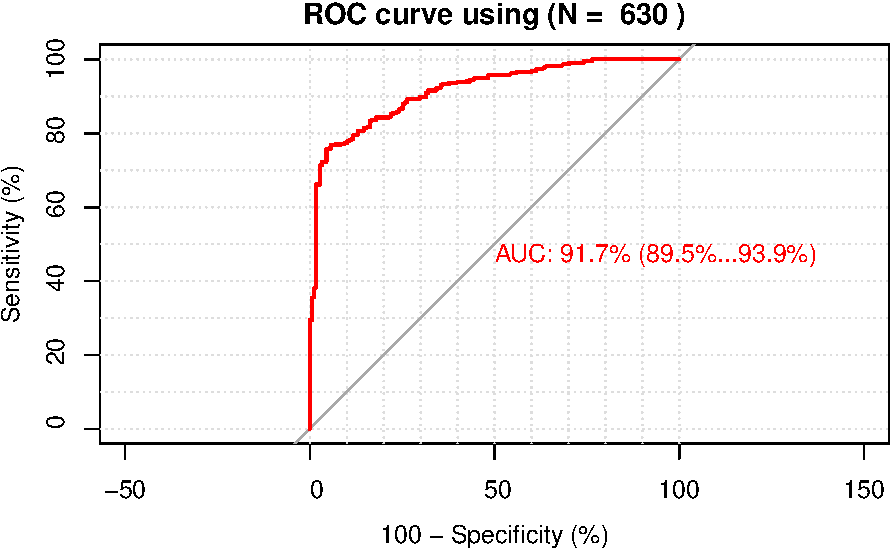
\includegraphics[width=0.95\linewidth]{EcoStat_files/figure-latex/fishing3-1} \caption{Application of the ROC methodology on the fishing-mode dataset.}\label{fig:fishing3}
\end{figure}

\end{example}

\hypertarget{TS}{%
\chapter{Time Series}\label{TS}}

\hypertarget{introduction-to-time-series}{%
\section{Introduction to time series}\label{introduction-to-time-series}}

A time series is an infinite sequence of random variables indexed by time: \(\{y_t\}_{t=-\infty}^{+\infty}=\{\dots, y_{-2},y_{-1},y_{0},y_{1},\dots,y_t,\dots\}\), \(y_i \in \mathbb{R}^k\). In practice, we only observe samples, typically: \(\{y_{1},\dots,y_T\}\).

Standard time series models are built using \textbf{shocks} that we will often denote by \(\varepsilon_t\). Typically, \(\mathbb{E}(\varepsilon_t)=0\). In many models, the shocks are supposed to be i.i.d., but there exist other (less restrictive) notions of shocks. In particular, the definition of many processes is based on whote noises:

\begin{definition}[White noise]
\protect\hypertarget{def:whitenoise}{}\label{def:whitenoise}

The process \(\{\varepsilon_t\}_{t \in] -\infty,+\infty[}\) is a white noise if, for all \(t\):

\begin{enumerate}
\def\labelenumi{\alph{enumi}.}
\tightlist
\item
  \(\mathbb{E}(\varepsilon_t)=0\),
\item
  \(\mathbb{E}(\varepsilon_t^2)=\sigma^2<\infty\) and
\item
  for all \(s\ne t\), \(\mathbb{E}(\varepsilon_t \varepsilon_s)=0\).
\end{enumerate}

\end{definition}

Another type of shocks that are commonly used are Martingale Difference Sequences:

\begin{definition}[Martingale Difference Sequence]
\protect\hypertarget{def:MDS}{}\label{def:MDS}The process \(\{\varepsilon_t\}_{t = -\infty}^{+\infty}\) is a martingale difference sequence (MDS) if \(\mathbb{E}(|\varepsilon_{t}|)<\infty\) and if, for all \(t\),
\[
\underbrace{\mathbb{E}_{t-1}(\varepsilon_{t})}_{\mbox{Expectation conditional on the past}}=0.
\]
\end{definition}

By definition, if \(y_t\) is a martingale, then \(y_{t}-y_{t-1}\) is a MDS.

\begin{example}[ARCH process]
\protect\hypertarget{exm:ARCH}{}\label{exm:ARCH}The Autoregressive conditional heteroskedasticity (ARCH) process is an example of shock that satisfies the MDS definition but that is not i.i.d.:
\[
\varepsilon_{t} = \sigma_t \times z_{t},
\]
where \(z_t \sim i.i.d.\,\mathcal{N}(0,1)\) and \(\sigma_t^2 = w + \alpha \varepsilon_{t-1}^2\).
\end{example}

\begin{example}
\protect\hypertarget{exm:whiteNotMDS}{}\label{exm:whiteNotMDS}A white noise process is not necessarily a MDS. This is for instance the following process:
\[
\varepsilon_{t} = z_t + z_{t-1}z_{t-2},
\]
where \(z_t \sim i.i.d.\mathcal{N}(0,1)\).
\end{example}

Let us now introduce the lag operator. The lag operator, denoted by \(L\), is defined on the time series space and is defined by:
\begin{equation}
L: \{y_t\}_{t=-\infty}^{+\infty} \rightarrow \{w_t\}_{t=-\infty}^{+\infty} \quad \mbox{with} \quad w_t = y_{t-1}.\label{eq:lagOp}
\end{equation}

We have: \(L^2 y_t = y_{t-2}\) and, more generally, \(L^k y_t = y_{t-k}\).

Consider a time series \(y_t\) defined by \(y_t = \mu + \phi y_{t-1} + \varepsilon_t\), where the \(\varepsilon_t\)'s are i.i.d. \(\mathcal{N}(0,\sigma^2)\). Using the lag operator, the dynamics of \(y_t\) can be expressed as follows:
\[
(1-\phi L) y_t = \mu + \varepsilon_t.
\]

It is easily checked that we have \(L^2 y_t = y_{t-2}\) and, generally, \(L^k y_t = y_{t-k}\).

If it exists, the \textbf{unconditional (or marginal) mean} of the random variable \(y_t\) is given by:
\[
\mu_t := \mathbb{E}(y_t) = \int_{-\infty}^{\infty} y_t f_{Y_t}(y_t) dy_t,
\]
where \(f_{Y_t}\) is the unconditional (or marginal) density of \(y_t\). Similarly, if it exists, the \textbf{unconditional (or marginal) variance} of the random variable \(y_t\) is:
\[
\mathbb{V}ar(y_t) = \int_{-\infty}^{\infty} (y_t - \mathbb{E}(y_t))^2 f_{Y_t}(y_t) dy_t.
\]

\begin{definition}[Autocovariance]
\protect\hypertarget{def:autocov}{}\label{def:autocov}The \(j^{th}\) autocovariance of \(y_t\) is given by:
\begin{eqnarray*}
\gamma_{j,t} &:=& \int_{-\infty}^{\infty} \int_{-\infty}^{\infty} \dots \int_{-\infty}^{\infty} [y_t - \mathbb{E}(y_t)][y_{t-j} - \mathbb{E}(y_{t-j})] \times\\
&& f_{Y_t,Y_{t-1},\dots,Y_{t-j}}(y_t,y_{t-1},\dots,y_{t-j}) dy_t dy_{t-1} \dots dy_{t-j} \\
&=& \mathbb{E}([y_t - \mathbb{E}(y_t)][y_{t-j} - \mathbb{E}(y_{t-j})]),
\end{eqnarray*}
where \(f_{Y_t,Y_{t-1},\dots,Y_{t-j}}(y_t,y_{t-1},\dots,y_{t-j})\) is the joint distribution of \(y_t,y_{t-1},\dots,y_{t-j}\).
\end{definition}

In particular, \(\gamma_{0,t} = \mathbb{V}ar(y_t)\).

\begin{definition}[Covariance stationarity]
\protect\hypertarget{def:covstat}{}\label{def:covstat}The process \(y_t\) is covariance stationary ---or weakly stationary--- if, for all \(t\) and \(j\),
\[
\mathbb{E}(y_t) = \mu \quad \mbox{and} \quad \mathbb{E}\{(y_t - \mu)(y_{t-j} - \mu)\} = \gamma_j.
\]
\end{definition}

Figure \ref{fig:nonstat1} displays the simulation of a process that is not covariance stationary. This process follows \(y_t = 0.1t + \varepsilon_t\), where \(\varepsilon_t \sim\,i.i.d.\,\mathcal{N}(0,1)\). Indeed, for such a process, we have: \(\mathbb{E}(y_t)=0.1t\), which depends on \(t\).

\begin{figure}
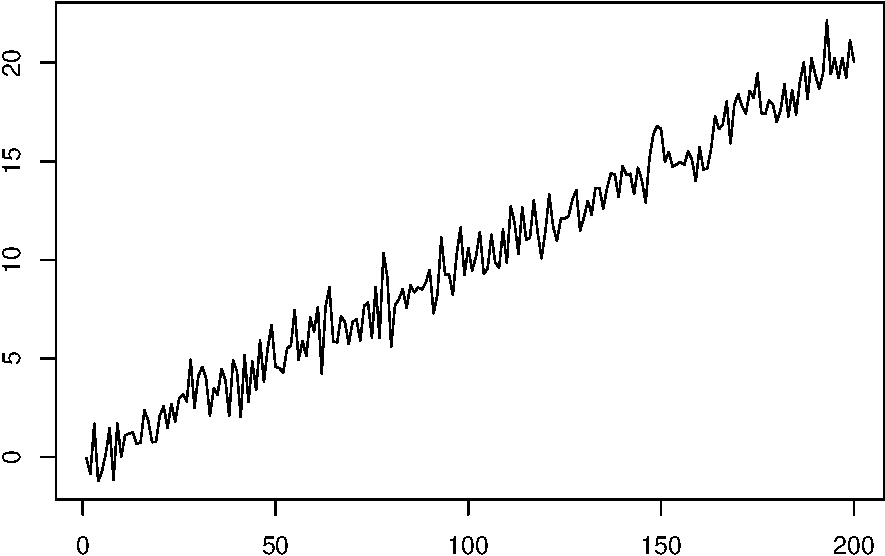
\includegraphics[width=0.95\linewidth]{EcoStat_files/figure-latex/nonstat1-1} \caption{Example of a process that is not covariance stationary ($y_t = 0.1t + \varepsilon_t$, where $\varepsilon_t \sim \mathcal{N}(0,1)$).}\label{fig:nonstat1}
\end{figure}

\begin{definition}[Strict stationarity]
\protect\hypertarget{def:strictstat}{}\label{def:strictstat}The process \(y_t\) is strictly stationary if, for all \(t\) and all sets of integers \(J=\{j_1,\dots,j_n\}\), the distribution of \((y_{t},y_{t+j_1},\dots,y_{t+j_n})\) depends on \(J\) but not on \(t\).
\end{definition}

The following process is covariance stationary but not strictly stationary:
\[
y_t = \mathbb{I}_{\{t<1000\}}\varepsilon_{1,t}+\mathbb{I}_{\{t\ge1000\}}\varepsilon_{2,t},
\]
where \(\varepsilon_{1,t} \sim \mathcal{N}(0,1)\) and \(\varepsilon_{2,t} \sim \sqrt{\frac{\nu - 2}{\nu}} t(\nu)\) and \(\nu = 4\).

\begin{figure}
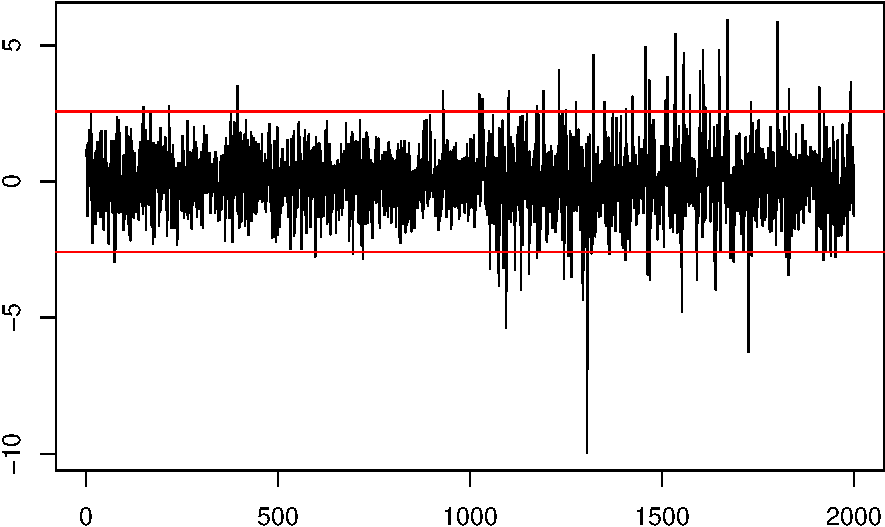
\includegraphics[width=0.95\linewidth]{EcoStat_files/figure-latex/nonstat2-1} \caption{Example of a process that is covariance stationary but not strictly stationary. The red lines delineate the 99\% confidence interval of the standard normal distribution ($\pm 2.58$).}\label{fig:nonstat2}
\end{figure}

\begin{proposition}
\protect\hypertarget{prp:gammaMinus}{}\label{prp:gammaMinus}If \(y_t\) is covariance stationary, then \(\gamma_j = \gamma_{-j}\).
\end{proposition}

\begin{proof}
Since \(y_t\) is covariance stationary, the covariance between \(y_t\) and \(y_{t-j}\) (i.e \(\gamma_j\)) is the same as that between \(y_{t+j}\) and \(y_{t+j-j}\) (i.e.~\(\gamma_{-j}\)).
\end{proof}

\begin{definition}[Auto-correlation]
\protect\hypertarget{def:autocor}{}\label{def:autocor}The \(j^{th}\) auto-correlation of a covariance-stationary process is:
\[
\rho_j = \frac{\gamma_j}{\gamma_0}.
\]
\end{definition}

Consider a long historical time series of the Swiss GDP growth, taken from the \citet{JST_2017} dataset.\footnote{Version 6 of the dataset, available on \href{https://www.macrohistory.net}{this website}.}

\begin{figure}
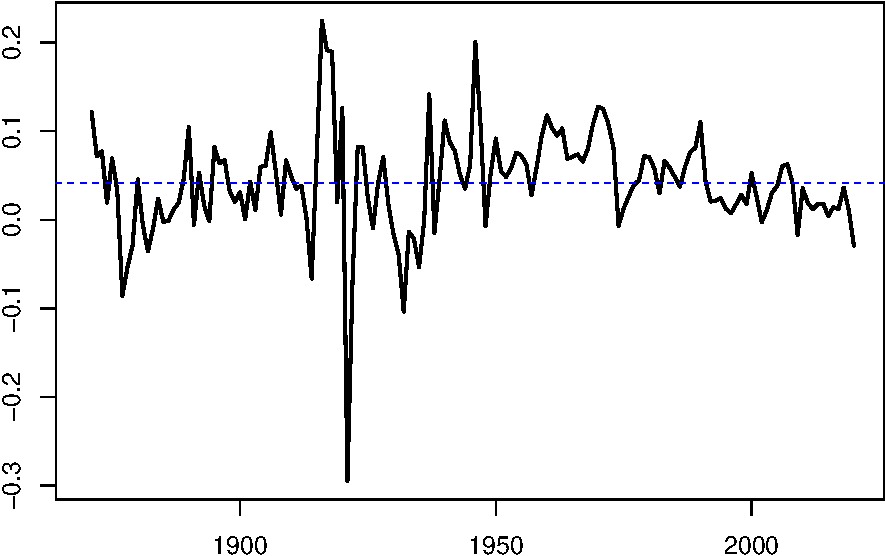
\includegraphics[width=0.95\linewidth]{EcoStat_files/figure-latex/autocov-1} \caption{Annual growth rate of Swiss GDP, based on the Jorda-Schularick-Taylor Macrohistory Database.}\label{fig:autocov}
\end{figure}

\begin{figure}
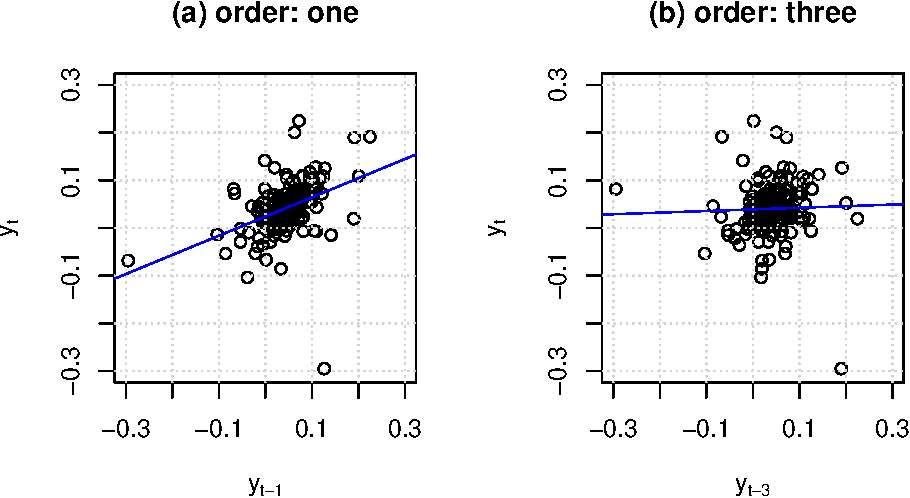
\includegraphics[width=0.95\linewidth]{EcoStat_files/figure-latex/autocov2-1} \caption{For order $j$, the slope of the blue line is, approximately, $\hat{\gamma}_j/\widehat{\mathbb{V}ar}(y_t)$, where hats indicate sample moments.}\label{fig:autocov2}
\end{figure}

\begin{definition}[Mean ergodicity]
\protect\hypertarget{def:ergodicity}{}\label{def:ergodicity}The covariance-stationary process \(y_t\) is ergodic for the mean if:
\[
\mbox{plim}_{T \rightarrow +\infty} \frac{1}{T}\sum_{t=1}^T y_t = \mathbb{E}(y_t).
\]
\end{definition}

\begin{definition}[Second-moment ergodicity]
\protect\hypertarget{def:ergod2nd}{}\label{def:ergod2nd}The covariance-stationary process \(y_t\) is ergodic for second moments if, for all \(j\):
\[
\mbox{plim}_{T \rightarrow +\infty} \frac{1}{T}\sum_{t=1}^T (y_t-\mu) (y_{t-j}-\mu) = \gamma_j.
\]
\end{definition}

It should be noted that ergodicity and stationarity are different properties. Typically if the process \(\{x_t\}\) is such that, \(\forall t\), \(x_t \equiv y\), where \(y \sim\,\mathcal{N}(0,1)\) (say), then \(\{x_t\}\) is stationary but not ergodic.

\begin{theorem}[Central Limit Theorem for covariance-stationary processes]
\protect\hypertarget{thm:CLTcovstat}{}\label{thm:CLTcovstat}If process \(y_t\) is covariance stationary and if the series of autocovariances is absolutely summable (\(\sum_{j=-\infty}^{+\infty} |\gamma_j| <\infty\)), then:
\begin{eqnarray}
\bar{y}_T \overset{m.s.}{\rightarrow} \mu &=& \mathbb{E}(y_t) \label{eq:TCL20}\\
\mbox{lim}_{T \rightarrow +\infty} T \mathbb{E}\left[(\bar{y}_T - \mu)^2\right] &=& \sum_{j=-\infty}^{+\infty} \gamma_j \label{eq:TCL2}\\
\sqrt{T}(\bar{y}_T - \mu) &\overset{d}{\rightarrow}& \mathcal{N}\left(0,\sum_{j=-\infty}^{+\infty} \gamma_j \right) \label{eq:TCL4ts}.
\end{eqnarray}

{[}Mean square (m.s.) and distribution (d.) convergences: see Definitions \ref{def:cvgceDistri} and \ref{def:convergenceLr}.{]}
\end{theorem}

\begin{proof}
By Proposition \ref{prp:absMs}, Eq. \eqref{eq:TCL2} implies Eq. \eqref{eq:TCL20}. For Eq. \eqref{eq:TCL2}, see Appendix \ref{AppendixProof}. For Eq. \eqref{eq:TCL4ts}, see \citet{Anderson_1971}, p.~429.
\end{proof}

\begin{definition}[Long-run variance]
\protect\hypertarget{def:LRV}{}\label{def:LRV}Under the assumptions of Theorem \ref{thm:CLTcovstat}, the limit appearing in Eq. \eqref{eq:TCL2} exists and is called \textbf{long-run variance}. It is denoted by \(S\), i.e.:
\[
S = \Sigma_{j=-\infty}^{+\infty} \gamma_j  = \mbox{lim}_{T \rightarrow +\infty} T \mathbb{E}[(\bar{y}_T - \mu)^2].
\]
\end{definition}

If \(y_t\) is ergodic for second moments (see Def. \ref{def:ergod2nd}), a natural estimator of \(S\) is:
\begin{equation}
\hat\gamma_0 + 2 \sum_{\nu=1}^{q} \hat\gamma_\nu, \label{eq:covSmplMean}
\end{equation}
where \(\hat\gamma_\nu = \frac{1}{T}\sum_{\nu+1}^{T} (y_t - \bar{y})(y_{t-\nu} - \bar{y})\).

However, for small samples, Eq. \eqref{eq:covSmplMean} does not necessarily result in a positive definite matrix. \citet{Newey_West_1987} have proposed an estimator that does not have this defect. Their estimator is given by:
\begin{equation}
S^{NW}=\hat\gamma_0 + 2 \sum_{\nu=1}^{q}\left(1-\frac{\nu}{q+1}\right) \hat\gamma_\nu.\label{eq:NWest}
\end{equation}

Loosely speaking, Theorem \ref{thm:CLTcovstat} says that, for a given sample size, the higher the ``persistency'' of a process, the lower the accuracy of the sample mean as an estimate of the population mean. To illustrate, consider three processes that feature the same marginal variance (equal to one, say), but different autocorrelations: 0\%, 70\%, and 99.9\%. Figure \ref{fig:TVTCL} displays simulated paths of such three processes. It indeed appears that, the larger the autocorrelation of the process, the further the sample mean (dashed red line) from the population mean (red solid line).

The same type of simulations can be performed using \href{https://jrenne.shinyapps.io/MacroEc/}{this ShinyApp} (use panel ``AR(1)'').

\begin{figure}
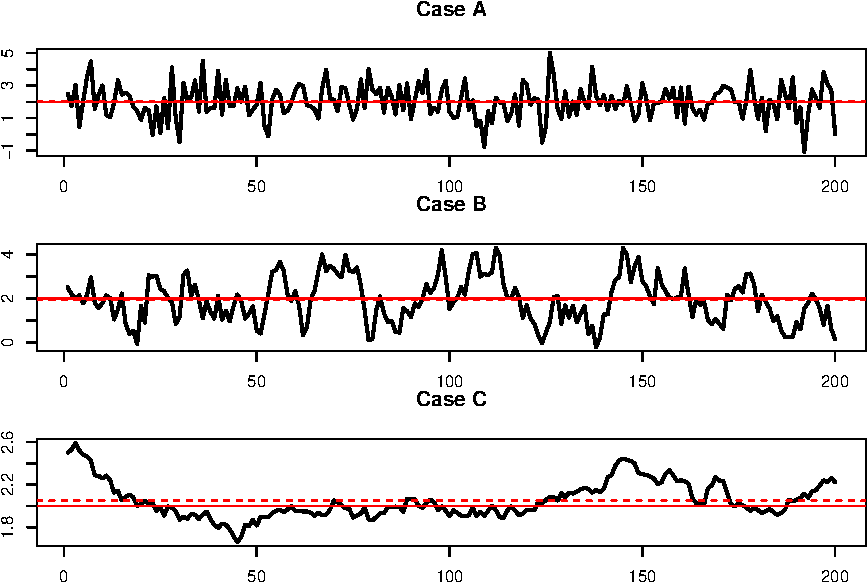
\includegraphics[width=1\linewidth]{EcoStat_files/figure-latex/TVTCL-1} \caption{The three samples have been simulated using the following data generating process: $x_t = \mu + \rho (x_{t-1}-\mu) + \sqrt{1-\rho^2}\varepsilon_t$, where $\varepsilon_t \sim \mathcal{N}(0,1)$. Case A: $\rho = 0$;  Case B: $\rho = 0.7$;  Case C: $\rho = 0.999$. In the three cases, $\mathbb{E}(x_t)=\mu=2$ and $\mathbb{V}ar(x_t)=1$.}\label{fig:TVTCL}
\end{figure}

\hypertarget{univariate-processes}{%
\section{Univariate processes}\label{univariate-processes}}

\hypertarget{moving-average-ma-processes}{%
\subsection{Moving Average (MA) processes}\label{moving-average-ma-processes}}

\begin{definition}
Consider a white noise process \(\{\varepsilon_t\}_{t = -\infty}^{+\infty}\) (Def. \ref{def:whitenoise}). Then \(y_t\) is a first-order moving average process if, for all \(t\):
\[
y_t = \mu + \varepsilon_t + \theta \varepsilon_{t-1}.
\]
\end{definition}

If \(\mathbb{E}(\varepsilon_t^2)=\sigma^2\), it is easily obtained that the unconditional mean and variances of \(y_t\) are:
\[
\mathbb{E}(y_t) = \mu, \quad \mathbb{V}ar(y_t) = (1+\theta^2)\sigma^2.
\]

The first auto-covariance is:
\[
\gamma_1=\mathbb{E}\{(y_t - \mu)(y_{t-1} - \mu)\} = \theta \sigma^2.
\]

Higher-order auto-covariances are zero (\(\gamma_j=0\) for \(j>1\)). Therefore: An MA(1) process is covariance-stationary (Def. \ref{def:covstat}).

For a MA(1) process, the autocorrelation of order \(j\) (see Def. \ref{def:autocor}) is given by:
\[
\rho_j =
\left\{
\begin{array}{lll}
1 &\mbox{ if }& j=0,\\
\theta / (1 + \theta^2) &\mbox{ if }& j = 1\\
0 &\mbox{ if }& j>1.
\end{array}
\right.
\]

Notice that process \(y_t\) defined through:
\[
y_t = \mu + \varepsilon_t +\theta \varepsilon_{t-1}, 
\]
where \(\mathbb{V}ar(\varepsilon_t)=\sigma^2\), has the same mean and autocovariances as
\[
y_t = \mu + \varepsilon^*_t +\frac{1}{\theta}\varepsilon^*_{t-1},
\]
where \(\mathbb{V}ar(\varepsilon^*_t)=\theta^2\sigma^2\). That is, even if we perfectly know the mean and auto-covariances of this process, it is not possible to identify which specification is the one that has been used to generate the data. Only one of these two specifications is said to be \emph{fundamental}, that is the one that satisfies \(|\theta_1|<1\).

\begin{definition}[MA(q) process]
\protect\hypertarget{def:MAq}{}\label{def:MAq}A \(q^{th}\) order Moving Average process is defined through:
\[
y_t = \mu + \varepsilon_t + \theta_1 \varepsilon_{t-1} + \dots + \theta_q \varepsilon_{t-q}.
\]
where \(\{\varepsilon_t\}_{t = -\infty}^{+\infty}\) is a white noise process (Def. \ref{def:whitenoise}).
\end{definition}

\begin{proposition}[Covariance-stationarity of an MA(q) process]
\protect\hypertarget{prp:covMAq}{}\label{prp:covMAq}Finite-order Moving Average processes are covariance-stationary.

Moreover, the autocovariances of an MA(q) process (as defined in Def. \ref{def:MAq}) are given by:
\begin{equation}
\gamma_j = \left\{ \begin{array}{ll} \sigma^2(\theta_j\theta_0 + \theta_{j+1}\theta_{1} +  \dots + \theta_{q}\theta_{q-j}) &\mbox{for} \quad j \in \{0,\dots,q\} \\ 0 &\mbox{for} \quad j>q, \end{array} \right.\label{eq:autocovMA}
\end{equation}
where we use the notation \(\theta_0=1\), and \(\mathbb{V}ar(\varepsilon_t)=\sigma^2\).
\end{proposition}

\begin{proof}
The unconditional expectation of \(y_t\) does not depend on time, since \(\mathbb{E}(y_t)=\mu\). Let's turn to autocovariances. We can extend the series of the \(\theta_j\)'s by setting \(\theta_j=0\) for \(j>q\). We then have:
\begin{eqnarray*}
\mathbb{E}((y_t-\mu)(y_{t-j}-\mu)) &=& \mathbb{E}\left[(\theta_0 \varepsilon_t +\theta_1 \varepsilon_{t-1} + \dots +\theta_j \varepsilon_{t-j}+\theta_{j+1} \varepsilon_{t-j-1} + \dots) \right.\times \\
&&\left. (\theta_0 \varepsilon_{t-j} +\theta_1 \varepsilon_{t-j-1} + \dots)\right].
\end{eqnarray*}
Then use the fact that \(\mathbb{E}(\varepsilon_t\varepsilon_s)=0\) if \(t \ne s\) (because \(\{\varepsilon_t\}_{t = -\infty}^{+\infty}\) is a white noise process).
\end{proof}

Figure \ref{fig:simMA} displays simulated paths of two MA processes (an MA(1) and an MA(4)). Such simulations can be produced by using panel ``ARMA(p,q)'' of \href{https://jrenne.shinyapps.io/MacroEc/}{this web interface}.

\begin{Shaded}
\begin{Highlighting}[]
\FunctionTok{library}\NormalTok{(AEC)}
\NormalTok{T }\OtherTok{\textless{}{-}} \DecValTok{100}\NormalTok{;nb.sim }\OtherTok{\textless{}{-}} \DecValTok{1}
\NormalTok{y}\FloatTok{.0} \OtherTok{\textless{}{-}} \FunctionTok{c}\NormalTok{(}\DecValTok{0}\NormalTok{)}
\NormalTok{c }\OtherTok{\textless{}{-}} \DecValTok{1}\NormalTok{;phi }\OtherTok{\textless{}{-}} \FunctionTok{c}\NormalTok{(}\DecValTok{0}\NormalTok{);sigma }\OtherTok{\textless{}{-}} \DecValTok{1}
\NormalTok{theta }\OtherTok{\textless{}{-}} \FunctionTok{c}\NormalTok{(}\DecValTok{1}\NormalTok{,}\DecValTok{1}\NormalTok{) }\CommentTok{\# MA(1) specification}
\NormalTok{y.sim }\OtherTok{\textless{}{-}} \FunctionTok{sim.arma}\NormalTok{(c,phi,theta,sigma,T,y}\FloatTok{.0}\NormalTok{,nb.sim)}
\FunctionTok{par}\NormalTok{(}\AttributeTok{mfrow=}\FunctionTok{c}\NormalTok{(}\DecValTok{1}\NormalTok{,}\DecValTok{2}\NormalTok{))}
\FunctionTok{par}\NormalTok{(}\AttributeTok{plt=}\FunctionTok{c}\NormalTok{(.}\DecValTok{2}\NormalTok{,.}\DecValTok{9}\NormalTok{,.}\DecValTok{2}\NormalTok{,.}\DecValTok{85}\NormalTok{))}
\FunctionTok{plot}\NormalTok{(y.sim[,}\DecValTok{1}\NormalTok{],}\AttributeTok{xlab=}\StringTok{""}\NormalTok{,}\AttributeTok{ylab=}\StringTok{""}\NormalTok{,}\AttributeTok{type=}\StringTok{"l"}\NormalTok{,}\AttributeTok{lwd=}\DecValTok{2}\NormalTok{,}
     \AttributeTok{main=}\FunctionTok{expression}\NormalTok{(}\FunctionTok{paste}\NormalTok{(theta[}\DecValTok{0}\NormalTok{],}\StringTok{"=1, "}\NormalTok{,theta[}\DecValTok{1}\NormalTok{],}\StringTok{"=1"}\NormalTok{,}\AttributeTok{sep=}\StringTok{""}\NormalTok{)))}
\FunctionTok{abline}\NormalTok{(}\AttributeTok{h=}\NormalTok{c)}
\NormalTok{theta }\OtherTok{\textless{}{-}} \FunctionTok{c}\NormalTok{(}\DecValTok{1}\NormalTok{,}\DecValTok{1}\NormalTok{,}\DecValTok{1}\NormalTok{,}\DecValTok{1}\NormalTok{,}\DecValTok{1}\NormalTok{) }\CommentTok{\# MA(4) specification}
\NormalTok{y.sim }\OtherTok{\textless{}{-}} \FunctionTok{sim.arma}\NormalTok{(c,phi,theta,sigma,T,y}\FloatTok{.0}\NormalTok{,nb.sim)}
\FunctionTok{plot}\NormalTok{(y.sim[,}\DecValTok{1}\NormalTok{],}\AttributeTok{xlab=}\StringTok{""}\NormalTok{,}\AttributeTok{ylab=}\StringTok{""}\NormalTok{,}\AttributeTok{type=}\StringTok{"l"}\NormalTok{,}\AttributeTok{lwd=}\DecValTok{2}\NormalTok{,}
     \AttributeTok{main=}\FunctionTok{expression}\NormalTok{(}\FunctionTok{paste}\NormalTok{(theta[}\DecValTok{0}\NormalTok{],}\StringTok{"=...="}\NormalTok{,theta[}\DecValTok{4}\NormalTok{],}\StringTok{"=1"}\NormalTok{,}\AttributeTok{sep=}\StringTok{""}\NormalTok{)))}
\FunctionTok{abline}\NormalTok{(}\AttributeTok{h=}\NormalTok{c)}
\end{Highlighting}
\end{Shaded}

\begin{figure}
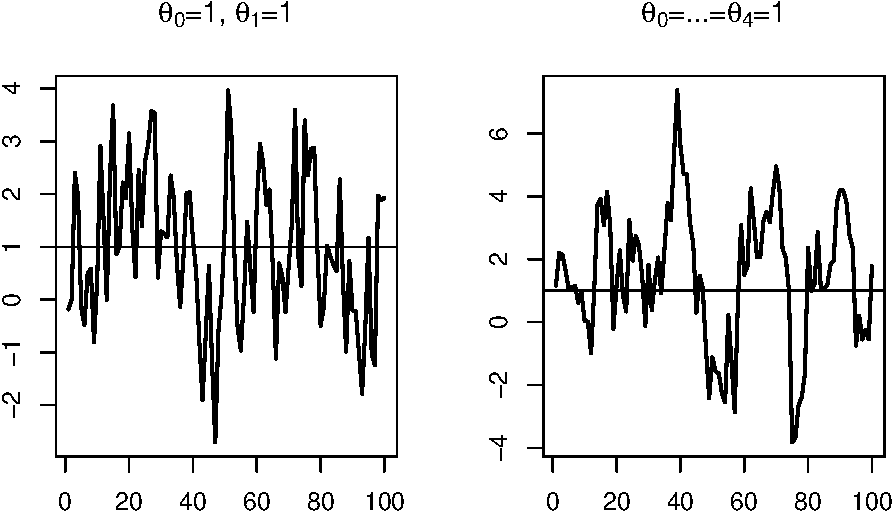
\includegraphics[width=0.95\linewidth]{EcoStat_files/figure-latex/simMA-1} \caption{Simulation of MA processes.}\label{fig:simMA}
\end{figure}

What if the order \(q\) of an MA(q) process gets infinite? The notion of \textbf{infinite-order Moving Average process} exists and is important in time series analysis. The (infinite) sequence of \(\theta_j\) has to satisfy some conditions for such a process to be well-defined (see Theorem \ref{thm:infMA} below). These conditions relate to the ``summability'' of \(\{\theta_{i}\}_{i\in\mathbb{N}}\) (see Definition \ref{def:summability}).

\begin{definition}[Absolute and square summability]
\protect\hypertarget{def:summability}{}\label{def:summability}The sequence \(\{\theta_{i}\}_{i\in\mathbb{N}}\) is absolutely summable if \(\sum_{i=0}^{\infty}|\theta_i| < + \infty\), and it is square summable if \(\sum_{i=0}^{\infty} \theta_i^2 < + \infty\).
\end{definition}

According to Prop. \ref{prp:absMs}, absolute summability implies square summability.

\begin{theorem}[Existence condition for an infinite MA process]
\protect\hypertarget{thm:infMA}{}\label{thm:infMA}If \(\{\theta_{i}\}_{i\in\mathbb{N}}\) is square summable (see Def. \ref{def:summability}) and if \(\{\varepsilon_t\}_{t = -\infty}^{+\infty}\) is a white noise process (see Def. \ref{def:whitenoise}), then
\[
\mu + \sum_{i=0}^{+\infty} \theta_{i} \varepsilon_{t-i}
\]
defines a well-behaved {[}covariance-stationary{]} process, called infinite-order MA process (MA(\(\infty\))).
\end{theorem}

\begin{proof}
See Appendix 3.A in Hamilton. ``Well behaved'' means that \(\Sigma_{i=0}^{T} \theta_{t-i} \varepsilon_{t-i}\) converges in mean square (Def. \ref{def:convergenceLr}) to some random variable \(Z_t\). The proof makes use of the fact that:
\[
\mathbb{E}\left[\left(\sum_{i=N}^{M}\theta_{i} \varepsilon_{t-i}\right)^2\right] = \sum_{i=N}^{M}|\theta_{i}|^2 \sigma^2,
\]
and that, when \(\{\theta_{i}\}\) is square summable, \(\forall \eta>0\), \(\exists N\) s.t. the right-hand-side term in the last equation is lower than \(\eta\) for all \(M \ge N\) (static Cauchy criterion, Theorem \ref{thm:cauchycritstatic}). This implies that \(\Sigma_{i=0}^{T} \theta_{i} \varepsilon_{t-i}\) converges in mean square (stochastic Cauchy criterion, see Theorem \ref{thm:cauchycritstochastic}).
\end{proof}

\begin{proposition}[First two moments of an infinite MA process]
\protect\hypertarget{prp:momentsMAinf}{}\label{prp:momentsMAinf}

If \(\{\theta_{i}\}_{i\in\mathbb{N}}\) is absolutely summable, i.e.~if \(\sum_{i=0}^{\infty}|\theta_i| < + \infty\), then

\begin{enumerate}
\def\labelenumi{\roman{enumi}.}
\tightlist
\item
  \(y_t = \mu + \sum_{i=0}^{+\infty} \theta_{i} \varepsilon_{t-i}\) exists (Theorem \ref{thm:infMA}) and is such that:
  \begin{eqnarray*}
  \mathbb{E}(y_t) &=& \mu\\
  \gamma_0 = \mathbb{E}([y_t-\mu]^2) &=& \sigma^2(\theta_0^2 +\theta_1^2 + \dots)\\
  \gamma_j = \mathbb{E}([y_t-\mu][y_{t-j}-\mu]) &=& \sigma^2(\theta_0\theta_j + \theta_{1}\theta_{j+1} + \dots).
  \end{eqnarray*}
\item
  Process \(y_t\) has absolutely summable auto-covariances, which implies that the results of Theorem \ref{thm:CLTcovstat} (Central Limit) apply.
\end{enumerate}

\end{proposition}

\begin{proof}
The absolute summability of \(\{\theta_{i}\}\) and the fact that \(\mathbb{E}(\varepsilon^2)<\infty\) imply that the order of integration and summation is interchangeable (see Hamilton, 1994, Footnote p.~52), which proves (i). For (ii), see end of Appendix 3.A in Hamilton (1994).
\end{proof}

\hypertarget{ARsection}{%
\subsection{Auto-Regressive (AR) processes}\label{ARsection}}

\begin{definition}[First-order AR process (AR(1))]
\protect\hypertarget{def:AR1}{}\label{def:AR1}Consider a white noise process \(\{\varepsilon_t\}_{t = -\infty}^{+\infty}\) (see Def. \ref{def:whitenoise}). Process \(y_t\) is an AR(1) process if it is defined by the following difference equation:
\[
y_t = c + \phi y_{t-1} + \varepsilon_t.
\]
\end{definition}

If \(|\phi|\ge1\), \(y_t\) is not stationary. Indeed, we have:
\[
y_{t+k} = c + \varepsilon_{t+k} + \phi  ( c + \varepsilon_{t+k-1})+ \phi^2  ( c + \varepsilon_{t+k-2})+ \dots + \phi^{k-1}  ( c + \varepsilon_{t+1}) + \phi^k y_t.
\]
Therefore, the conditional variance
\[
\mathbb{V}ar_t(y_{t+k}) = \sigma^2(1 + \phi^2 + \phi^4 + \dots + \phi^{2(k-1)})
\]
does not converge for large \(k\)'s. This implies that \(\mathbb{V}ar(y_{t})\) does not exist.

By contrast, if \(|\phi| < 1\), one can see that:
\[
y_t = c + \varepsilon_t + \phi  ( c + \varepsilon_{t-1})+ \phi^2  ( c + \varepsilon_{t-2})+ \dots + \phi^k  ( c + \varepsilon_{t-k}) + \dots
\]
Hence, if \(|\phi| < 1\), the unconditional mean and variance of \(y_t\) are:
\[
\mathbb{E}(y_t) = \frac{c}{1-\phi} =: \mu \quad \mbox{and} \quad \mathbb{V}ar(y_t) = \frac{\sigma^2}{1-\phi^2}.
\]

Let us compute the \(j^{th}\) autocovariance of the AR(1) process:
\begin{eqnarray*}
\mathbb{E}([y_{t} - \mu][y_{t-j} - \mu]) &=& \mathbb{E}([\varepsilon_t + \phi  \varepsilon_{t-1}+ \phi^2 \varepsilon_{t-2} + \dots + \color{red}{\phi^j \varepsilon_{t-j}} + \color{blue}{\phi^{j+1} \varepsilon_{t-j-1}} \dots]\times \\
&&[\color{red}{\varepsilon_{t-j}} + \color{blue}{\phi \varepsilon_{t-j-1}} + \phi^2 \varepsilon_{t-j-2} + \dots + \phi^k \varepsilon_{t-j-k} + \dots])\\
&=& \mathbb{E}(\color{red}{\phi^j \varepsilon_{t-j}^2}+\color{blue}{\phi^{j+2} \varepsilon_{t-j-1}^2}+\phi^{j+4} \varepsilon_{t-j-2}^2+\dots)\\
&=& \frac{\phi^j \sigma^2}{1 - \phi^2}.
\end{eqnarray*}

Therefore \(\rho_j = \phi^j\).

By what precedes, we have:

\begin{proposition}[Covariance-stationarity of an AR(1) process]
\protect\hypertarget{prp:statioAR1}{}\label{prp:statioAR1}The AR(1) process, as defined in Def. \ref{def:AR1}, is covariance-stationary iff \(|\phi|<1\).
\end{proposition}

\begin{definition}[AR(p) process]
\protect\hypertarget{def:ARp}{}\label{def:ARp}Consider a white noise process \(\{\varepsilon_t\}_{t = -\infty}^{+\infty}\) (see Def. \ref{def:whitenoise}). Process \(y_t\) is a \(p^{th}\)-order autoregressive process (AR(p)) if its dynamics is defined by the following difference equation (with \(\phi_p \ne 0\)):
\begin{equation}
y_t = c + \phi_1 y_{t-1} + \phi_2 y_{t-2} + \dots + \phi_p y_{t-p} + \varepsilon_t.\label{eq:AR}
\end{equation}
\end{definition}

As we will see, the covariance-stationarity of process \(y_t\) hinges on matrix \(F\) defined as:
\begin{equation}
F = \left[
\begin{array}{ccccc}
\phi_1 & \phi_2 & \dots& & \phi_p \\
1 & 0 &\dots && 0 \\
0 & 1 &\dots && 0 \\
\vdots &  & \ddots && \vdots \\
0 & 0 &\dots &1& 0 \\
\end{array}
\right].\label{eq:F}
\end{equation}

Note that this matrix \(F\) is such that if \(y_t\) follows Eq. \eqref{eq:AR}, then process \(\mathbf{y}_t\) follows:
\[
\mathbf{y}_t = \mathbf{c} + F \mathbf{y}_{t-1} + \boldsymbol\xi_t
\]
with
\[
\mathbf{c} =
\left[\begin{array}{c}
c\\
0\\
\vdots\\
0
\end{array}\right],
\quad
\boldsymbol\xi_t =
\left[\begin{array}{c}
\varepsilon_t\\
0\\
\vdots\\
0
\end{array}\right],
\quad
\mathbf{y}_t =
\left[\begin{array}{c}
y_t\\
y_{t-1}\\
\vdots\\
y_{t-p+1}
\end{array}\right].
\]

\begin{proposition}[The eigenvalues of matrix F]
\protect\hypertarget{prp:Feigen}{}\label{prp:Feigen}The eigenvalues of \(F\) (defined by Eq. \eqref{eq:F}) are the solutions of:
\begin{equation}
\lambda^p - \phi_1 \lambda^{p-1} - \dots - \phi_{p-1}\lambda - \phi_p = 0.\label{eq:Feigen}
\end{equation}
\end{proposition}

\begin{proposition}[Covariance-stationarity of an AR(p) process]
\protect\hypertarget{prp:stability}{}\label{prp:stability}

These four statements are equivalent:

\begin{enumerate}
\def\labelenumi{\roman{enumi}.}
\tightlist
\item
  Process \(\{y_t\}\), defined in Def. \ref{def:ARp}, is covariance-stationary.
\item
  The eigenvalues of \(F\) (as defined Eq. \eqref{eq:F}) lie strictly within the unit circle.
\item
  The roots of Eq. \eqref{eq:outside} (below) lie strictly outside the unit circle.
  \begin{equation}
  1 - \phi_1 z - \dots - \phi_{p-1}z^{p-1} - \phi_p z^p = 0.\label{eq:outside}
  \end{equation}
\item
  The roots of Eq. \eqref{eq:inside} (below) lie strictly inside the unit circle.
  \begin{equation}
  \lambda^p - \phi_1 \lambda^{p-1} - \dots - \phi_{p-1}\lambda - \phi_p = 0.\label{eq:inside}
  \end{equation}
\end{enumerate}

\end{proposition}

\begin{proof}
We consider the case where the eigenvalues of \(F\) are distinct; Jordan decomposition can be used in the general case. When the eigenvalues of \(F\) are distinct, \(F\) admits the following spectral decomposition: \(F = PDP^{-1}\), where \(D\) is diagonal. Using the notations introduced in Eq. \eqref{eq:F}, we have:
\[
\mathbf{y}_{t} = \mathbf{c} + F \mathbf{y}_{t-1} + \boldsymbol\xi_{t}.
\]
Let's introduce \(\mathbf{d} = P^{-1}\mathbf{c}\), \(\mathbf{z}_t = P^{-1}\mathbf{y}_t\) and \(\boldsymbol\eta_t = P^{-1}\boldsymbol\xi_t\). We have:
\[
\mathbf{z}_{t} = \mathbf{d} + D \mathbf{z}_{t-1} + \boldsymbol\eta_{t}.
\]
Because \(D\) is diagonal, the different component of \(\mathbf{z}_t\), denoted by \(z_{i,t}\), follow AR(1) processes. The (scalar) autoregressive parameters of these AR(1) processes are the diagonal entries of \(D\) --which also are the eigenvalues of \(F\)-- that we denote by \(\lambda_i\).

Process \(y_t\) is covariance-stationary iff \(\mathbf{y}_{t}\) also is covariance-stationary, which is the case iff all \(z_{i,t}\), \(i \in [1,p]\), are covariance-stationary. By Prop. \ref{prp:statioAR1}, process \(z_{i,t}\) is covariance-stationary iff \(|\lambda_i|<1\). This proves that (i) is equivalent to (ii). Prop. \ref{prp:Feigen} further proves that (ii) is equivalent to (iv). Finally, it is easily seen that (iii) is equivalent to (iv) (as long as \(\phi_p \ne 0\)).
\end{proof}

Using the lag operator (see Eq \eqref{eq:lagOp}), if \(y_t\) is a covariance-stationary AR(p) process (Def. \ref{def:ARp}), we can write:
\[
y_t = \mu + \psi(L)\varepsilon_t,
\]
where
\begin{equation}
\psi(L) = (1 - \phi_1 L - \dots - \phi_p L^p)^{-1},
\end{equation}
and
\begin{equation}
\mu = \mathbb{E}(y_t) = \dfrac{c}{1-\phi_1 -\dots - \phi_p}.\label{eq:EAR}
\end{equation}

In the following lines of codes, we compute the eigenvalues of the \(F\) matrices associated with the following processes (where \(\varepsilon_t\) is a white noise):
\begin{eqnarray*}
x_t &=& 0.9 x_{t-1} -0.2 x_{t-2} + \varepsilon_t\\
y_t &=& 1.1 y_{t-1} -0.3 y_{t-2} + \varepsilon_t\\
w_t &=& 1.4 w_{t-1} -0.7 w_{t-2} + \varepsilon_t\\
z_t &=& 0.9 z_{t-1} +0.2 z_{t-2} + \varepsilon_t
\end{eqnarray*}

\begin{Shaded}
\begin{Highlighting}[]
\NormalTok{F }\OtherTok{\textless{}{-}} \FunctionTok{matrix}\NormalTok{(}\FunctionTok{c}\NormalTok{(.}\DecValTok{9}\NormalTok{,}\DecValTok{1}\NormalTok{,}\SpecialCharTok{{-}}\NormalTok{.}\DecValTok{2}\NormalTok{,}\DecValTok{0}\NormalTok{),}\DecValTok{2}\NormalTok{,}\DecValTok{2}\NormalTok{)}
\NormalTok{lambda\_x }\OtherTok{\textless{}{-}} \FunctionTok{eigen}\NormalTok{(F)}\SpecialCharTok{$}\NormalTok{values}
\NormalTok{F[}\DecValTok{1}\NormalTok{,] }\OtherTok{\textless{}{-}} \FunctionTok{c}\NormalTok{(}\FloatTok{1.1}\NormalTok{,}\SpecialCharTok{{-}}\NormalTok{.}\DecValTok{3}\NormalTok{)}
\NormalTok{lambda\_y }\OtherTok{\textless{}{-}} \FunctionTok{eigen}\NormalTok{(F)}\SpecialCharTok{$}\NormalTok{values}
\NormalTok{F[}\DecValTok{1}\NormalTok{,] }\OtherTok{\textless{}{-}} \FunctionTok{c}\NormalTok{(}\FloatTok{1.4}\NormalTok{,}\SpecialCharTok{{-}}\NormalTok{.}\DecValTok{7}\NormalTok{)}
\NormalTok{lambda\_w }\OtherTok{\textless{}{-}} \FunctionTok{eigen}\NormalTok{(F)}\SpecialCharTok{$}\NormalTok{values}
\NormalTok{F[}\DecValTok{1}\NormalTok{,] }\OtherTok{\textless{}{-}} \FunctionTok{c}\NormalTok{(.}\DecValTok{9}\NormalTok{,.}\DecValTok{2}\NormalTok{)}
\NormalTok{lambda\_z }\OtherTok{\textless{}{-}} \FunctionTok{eigen}\NormalTok{(F)}\SpecialCharTok{$}\NormalTok{values}
\FunctionTok{rbind}\NormalTok{(lambda\_x,lambda\_y,lambda\_w,lambda\_z)}
\end{Highlighting}
\end{Shaded}

\begin{verbatim}
##                         [,1]                  [,2]
## lambda_x 0.500000+0.0000000i  0.4000000+0.0000000i
## lambda_y 0.600000+0.0000000i  0.5000000+0.0000000i
## lambda_w 0.700000+0.4582576i  0.7000000-0.4582576i
## lambda_z 1.084429+0.0000000i -0.1844289+0.0000000i
\end{verbatim}

The absolute values of the eigenvalues associated with process \(w_t\) are both equal to 0.837. Therefore, according to Proposition \ref{prp:stability}, processes \(x_t\), \(y_t\), and \(w_t\) are covariance-stationary, but not \(z_t\) (because the absolute value of one of the eigenvalues of the \(F\) matrix associated with this process is larger than 1).

The computation of the autocovariances of \(y_t\) is based on the so-called \textbf{Yule-Walker equations} (Eq. \eqref{eq:gammas}). Let's rewrite Eq. \eqref{eq:AR}:
\[
(y_t-\mu) = \phi_1 (y_{t-1}-\mu) + \phi_2 (y_{t-2}-\mu) + \dots + \phi_p (y_{t-p}-\mu) + \varepsilon_t.
\]
Multiplying both sides by \(y_{t-j}-\mu\) and taking expectations leads to the (Yule-Walker) equations:
\begin{equation}
\gamma_j = \left\{
\begin{array}{l}
\phi_1 \gamma_{j-1}+\phi_2 \gamma_{j-2}+ \dots + \phi_p \gamma_{j-p} \quad if \quad j>0\\
\phi_1 \gamma_{1}+\phi_2 \gamma_{2}+ \dots + \phi_p \gamma_{p} + \sigma^2 \quad for \quad j=0.
\end{array}
\right.\label{eq:gammas}
\end{equation}
Using \(\gamma_j = \gamma_{-j}\) (Prop. \ref{prp:gammaMinus}), one can express \((\gamma_0,\gamma_1,\dots,\gamma_{p})\) as functions of \((\sigma^2,\phi_1,\dots,\phi_p)\).

\hypertarget{PACFapproach}{%
\subsection{PACF approach to identify AR/MA processes}\label{PACFapproach}}

We have seen that the \(k^{th}\)-order auto-correlation of a MA(q) process is null if \(k>q\). This is exploited, in practice, to determine the order of a MA process. Moreover, since this is not the case for an AR process, this can be used to distinguish an AR from an MA process.

There exists an equivalent approach to determine whether a process can be modeled as an AR process; it is based on partial auto-correlations:

\begin{definition}[Partial auto-correlation]
\protect\hypertarget{def:partialAC}{}\label{def:partialAC}In a time series context, the partial auto-correlation (\(\phi_{h,h}\)) of process \(\{y_t\}\) is defined as the partial correlation of \(y_{t+h}\) and \(y_t\) given \(y_{t+h-1},\dots,y_{t+1}\). (see Def. \ref{def:partialcorrel} for the definition of partial correlation.)
\end{definition}

If \(h>p\), the regression of \(y_{t+h}\) on \(y_{t+h-1},\dots,y_{t+1}\) is:
\[
y_{t+h} = c + \phi_1 y_{t+h-1}+\dots+ \phi_p  y_{t+h-p} + \varepsilon_{t+h}.
\]
The residuals of the latter regressions (\(\varepsilon_{t+h}\)) are uncorrelated to \(y_t\). Then the partial autocorrelation is zero for \(h>p\).

Besides, it can be shown that \(\phi_{p,p}=\phi_p\). Hence \(\phi_{p,p}=\phi_p\) but \(\phi_{h,h}=0\) for \(h>p\). This can be used to determine the order of an AR process. By contrast (importantly) if \(y_t\) follows an MA(q) process, then \(\phi_{k,k}\) asymptotically approaches zero instead of cutting off abruptly.

As illustrated below, functions \texttt{acf} and \texttt{pacf} can be conveniently used to employ the (P)ACF approach. (Note also the use of function \texttt{sim.arma} to simulate ARMA processes.)

\begin{Shaded}
\begin{Highlighting}[]
\FunctionTok{library}\NormalTok{(AEC)}
\FunctionTok{par}\NormalTok{(}\AttributeTok{mfrow=}\FunctionTok{c}\NormalTok{(}\DecValTok{3}\NormalTok{,}\DecValTok{2}\NormalTok{))}
\FunctionTok{par}\NormalTok{(}\AttributeTok{plt=}\FunctionTok{c}\NormalTok{(.}\DecValTok{2}\NormalTok{,.}\DecValTok{9}\NormalTok{,.}\DecValTok{2}\NormalTok{,.}\DecValTok{95}\NormalTok{))}
\NormalTok{theta }\OtherTok{\textless{}{-}} \FunctionTok{c}\NormalTok{(}\DecValTok{1}\NormalTok{,}\DecValTok{2}\NormalTok{,}\DecValTok{1}\NormalTok{);phi}\OtherTok{=}\DecValTok{0}
\NormalTok{y.sim }\OtherTok{\textless{}{-}} \FunctionTok{sim.arma}\NormalTok{(}\AttributeTok{c=}\DecValTok{0}\NormalTok{,phi,theta,}\AttributeTok{sigma=}\DecValTok{1}\NormalTok{,}\AttributeTok{T=}\DecValTok{1000}\NormalTok{,}\AttributeTok{y.0=}\DecValTok{0}\NormalTok{,}\AttributeTok{nb.sim=}\DecValTok{1}\NormalTok{)}
\FunctionTok{par}\NormalTok{(}\AttributeTok{mfg=}\FunctionTok{c}\NormalTok{(}\DecValTok{1}\NormalTok{,}\DecValTok{1}\NormalTok{));}\FunctionTok{plot}\NormalTok{(y.sim,}\AttributeTok{type=}\StringTok{"l"}\NormalTok{,}\AttributeTok{lwd=}\DecValTok{2}\NormalTok{)}
\FunctionTok{par}\NormalTok{(}\AttributeTok{mfg=}\FunctionTok{c}\NormalTok{(}\DecValTok{2}\NormalTok{,}\DecValTok{1}\NormalTok{));}\FunctionTok{acf}\NormalTok{(y.sim)}
\FunctionTok{par}\NormalTok{(}\AttributeTok{mfg=}\FunctionTok{c}\NormalTok{(}\DecValTok{3}\NormalTok{,}\DecValTok{1}\NormalTok{));}\FunctionTok{pacf}\NormalTok{(y.sim)}
\NormalTok{theta }\OtherTok{\textless{}{-}} \FunctionTok{c}\NormalTok{(}\DecValTok{1}\NormalTok{);phi}\OtherTok{=}\FloatTok{0.9}
\NormalTok{y.sim }\OtherTok{\textless{}{-}} \FunctionTok{sim.arma}\NormalTok{(}\AttributeTok{c=}\DecValTok{0}\NormalTok{,phi,theta,}\AttributeTok{sigma=}\DecValTok{1}\NormalTok{,}\AttributeTok{T=}\DecValTok{1000}\NormalTok{,}\AttributeTok{y.0=}\DecValTok{0}\NormalTok{,}\AttributeTok{nb.sim=}\DecValTok{1}\NormalTok{)}
\FunctionTok{par}\NormalTok{(}\AttributeTok{mfg=}\FunctionTok{c}\NormalTok{(}\DecValTok{1}\NormalTok{,}\DecValTok{2}\NormalTok{));}\FunctionTok{plot}\NormalTok{(y.sim,}\AttributeTok{type=}\StringTok{"l"}\NormalTok{,}\AttributeTok{lwd=}\DecValTok{2}\NormalTok{)}
\FunctionTok{par}\NormalTok{(}\AttributeTok{mfg=}\FunctionTok{c}\NormalTok{(}\DecValTok{2}\NormalTok{,}\DecValTok{2}\NormalTok{));}\FunctionTok{acf}\NormalTok{(y.sim)}
\FunctionTok{par}\NormalTok{(}\AttributeTok{mfg=}\FunctionTok{c}\NormalTok{(}\DecValTok{3}\NormalTok{,}\DecValTok{2}\NormalTok{));}\FunctionTok{pacf}\NormalTok{(y.sim)}
\end{Highlighting}
\end{Shaded}

\begin{figure}
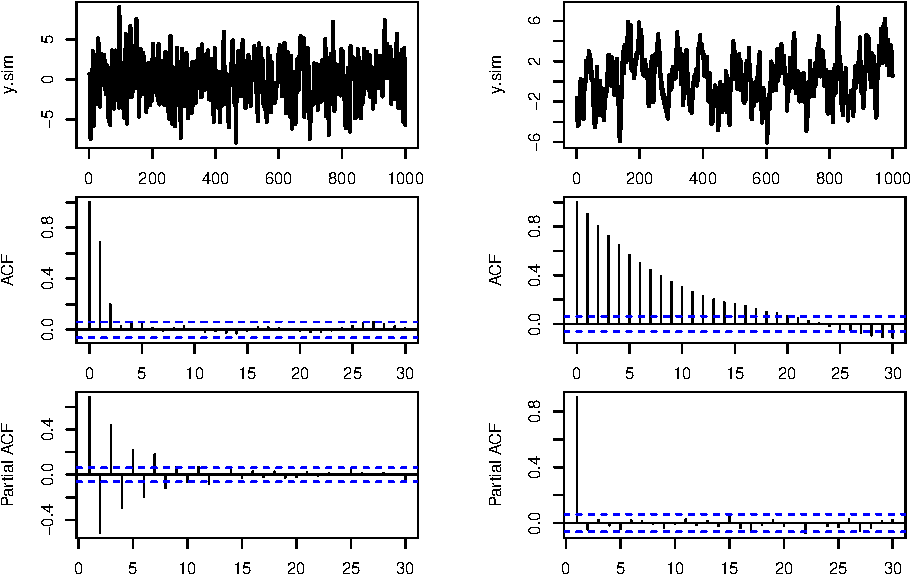
\includegraphics[width=1\linewidth]{EcoStat_files/figure-latex/pacf-1} \caption{ACF/PACF analysis of two processes (MA process on the left, AR on the right).}\label{fig:pacf}
\end{figure}

\hypertarget{forecasting}{%
\section{Forecasting}\label{forecasting}}

Forecasting has always been an important part of the time series field (\citet{DEGOOIJER2006443}). Macroeconomic forecasts are done in many places: Public Administration (notably Treasuries), Central Banks, International Institutions (e.g.~IMF, OECD), banks, big firms. These institutions are interested in the \textbf{point estimates} (\(\sim\) most likely value) of the variable of interest. They also sometimes need to measure the \textbf{uncertainty} (\(\sim\) dispersion of likely outcomes) associated to the point estimates.\footnote{In its inflation report, the Bank of England displays charts showing the conditional distribution of future inflation, called fan charts. This fan charts show the uncertainty associated with future inflation. See \href{https://www.bankofengland.co.uk/quarterly-bulletin/1998/q1/the-inflation-report-projections-understanding-the-fan-chart}{this page}.}

Forecasts produced by professional forecasters are available on these web pages:

\begin{itemize}
\tightlist
\item
  \href{https://www.philadelphiafed.org/research-and-data/real-time-center/survey-of-professional-forecasters/}{Philly Fed Survey of Professional Forecasters}.
\item
  \href{http://www.ecb.europa.eu/stats/prices/indic/forecast/html/index.en.html}{ECB Survey of Professional Forecasters}.
\item
  \href{https://www.imf.org/external/pubs/ft/weo/2016/update/01/}{IMF World Economic Outlook}.
\item
  \href{http://www.oecd.org/eco/economicoutlook.htm}{OECD Global Economic Outlook}.
\item
  \href{http://ec.europa.eu/economy_finance/eu/forecasts/index_en.htm}{European Commission Economic Forecasts}.
\end{itemize}

How to formalize the forecasting problem? Assume the current date is \(t\). We want to forecast the value that variable \(y_t\) will take on date \(t+1\) (i.e., \(y_{t+1}\)) based on the observation of a set of variables gathered in vector \(x_t\) (\(x_t\) may contain lagged values of \(y_t\)).

The forecaster aims at minimizing (a function of) the forecast error. It is usal to consider the following (quadratic) loss function:
\[
\underbrace{\mathbb{E}([y_{t+1} - y^*_{t+1}]^2)}_{\mbox{Mean square error (MSE)}}
\]
where \(y^*_{t+1}\) is the forecast of \(y_{t+1}\) (function of \(x_t\)).

\begin{proposition}[Smallest MSE]
\protect\hypertarget{prp:smallestMSE}{}\label{prp:smallestMSE}The smallest MSE is obtained with MSEthe expectation of \(y_{t+1}\) conditional on \(x_t\).
\end{proposition}

\begin{proof}
See Appendix \ref{AppendixProof}.
\end{proof}

\begin{proposition}
\protect\hypertarget{prp:smallestMSElinear}{}\label{prp:smallestMSElinear}Among the class of linear forecasts, the smallest MSE is obtained with the linear projection of \(y_{t+1}\) on \(x_t\).
This projection, denoted by \(\hat{P}(y_{t+1}|x_t):=\boldsymbol\alpha'x_t\), satisfies:
\begin{equation}
\mathbb{E}\left( [y_{t+1} - \boldsymbol\alpha'x_t]x_t \right)=\mathbf{0}.\label{eq:proj}
\end{equation}
\end{proposition}

\begin{proof}
Consider the function \(f:\) \(\boldsymbol\alpha \rightarrow \mathbb{E}\left( [y_{t+1} - \boldsymbol\alpha'x_t]^2 \right)\). We have:
\[
f(\boldsymbol\alpha) = \mathbb{E}\left( y_{t+1}^2 - 2 y_t x_t'\boldsymbol\alpha + \boldsymbol\alpha'x_t x_t'\boldsymbol\alpha] \right).
\]
We have \(\partial f(\boldsymbol\alpha)/\partial \boldsymbol\alpha = \mathbb{E}(-2 y_{t+1} x_t + 2 x_t x_t'\boldsymbol\alpha)\). The function is minimised for \(\partial f(\boldsymbol\alpha)/\partial \boldsymbol\alpha =0\).
\end{proof}

Eq. \eqref{eq:proj} implies that \(\mathbb{E}\left( y_{t+1}x_t \right)=\mathbb{E}\left(x_tx_t' \right)\boldsymbol\alpha\). (Note that \(x_t x_t'\boldsymbol\alpha=x_t (x_t'\boldsymbol\alpha)=(\boldsymbol\alpha'x_t) x_t'\).)

Hence, if \(\mathbb{E}\left(x_tx_t' \right)\) is nonsingular,
\begin{equation}
\boldsymbol\alpha=[\mathbb{E}\left(x_tx_t' \right)]^{-1}\mathbb{E}\left( y_{t+1}x_t \right).\label{eq:linproj}
\end{equation}

The MSE then is:
\[
\mathbb{E}([y_{t+1} - \boldsymbol\alpha'x_t]^2) = \mathbb{E}{(y_{t+1}^2)} - \mathbb{E}\left( y_{t+1}x_t' \right)[\mathbb{E}\left(x_tx_t' \right)]^{-1}\mathbb{E}\left(x_ty_{t+1} \right).
\]

Consider the regression \(y_{t+1} = \boldsymbol\beta'\mathbf{x}_t + \varepsilon_{t+1}\). The OLS estimate is:
\[
\mathbf{b} = \left[ \underbrace{ \frac{1}{T} \sum_{i=1}^T \mathbf{x}_t\mathbf{x}_t'}_{\mathbf{m}_1} \right]^{-1}\left[  \underbrace{ \frac{1}{T} \sum_{i=1}^T \mathbf{x}_t'y_{t+1}}_{\mathbf{m}_2} \right].
\]
If \(\{x_t,y_t\}\) is covariance-stationary and ergodic for the second moments then the sample moments (\(\mathbf{m}_1\) and \(\mathbf{m}_2\)) converges in probability to the associated population moments and \(\mathbf{b} \overset{p}{\rightarrow} \boldsymbol\alpha\) (where \(\boldsymbol\alpha\) is defined in Eq. \eqref{eq:linproj}).

\begin{example}[Forecasting an MA(q) process]
\protect\hypertarget{exm:fcstMAq}{}\label{exm:fcstMAq}Consider the MA(q) process:
\[
y_t = \mu + \varepsilon_t + \theta_1 \varepsilon_{t-1} + \dots + \theta_q \varepsilon_{t-q},
\]
where \(\{\varepsilon_t\}\) is a white noise sequence (Def. \ref{def:whitenoise}).

We have:\footnote{The present reasoning relies on the assumption that the \(\varepsilon_t\)'s are observed. But this is generally not the case in practice, where the \(\varepsilon_t\)'s generally have to be estimated.}
\begin{eqnarray*}
&&\mathbb{E}(y_{t+h}|\varepsilon_{t},\varepsilon_{t-1},\dots) =\\
&&\left\{
\begin{array}{lll}
\mu + \theta_h \varepsilon_{t} + \dots + \theta_q \varepsilon_{t-q+h}  \quad &for& \quad h \in [1,q]\\
\mu \quad &for& \quad h > q
\end{array}
\right.
\end{eqnarray*}
and
\begin{eqnarray*}
&&\mathbb{V}ar(y_{t+h}|\varepsilon_{t},\varepsilon_{t-1},\dots)= \mathbb{E}\left( [y_{t+h} - \mathbb{E}(y_{t+h}|\varepsilon_{t},\varepsilon_{t-1},\dots)]^2 \right) =\\
&&\left\{
\begin{array}{lll}
\sigma^2(1+\theta_1^2+\dots+\theta_{h-1}^2) \quad &for& \quad h \in [1,q]\\
\sigma^2(1+\theta_1^2+\dots+\theta_q^2) \quad &for& \quad h>q.
\end{array}
\right.
\end{eqnarray*}
\end{example}

\begin{example}[Forecasting an AR(p) process]
\protect\hypertarget{exm:fcstARp}{}\label{exm:fcstARp}(See \href{https://jrenne.shinyapps.io/ARpFcst}{this web interface}.) Consider the AR(p) process:
\[
y_t = c + \phi_1 y_{t-1} + \phi_2 y_{t-2} + \dots + \phi_p y_{t-p} + \varepsilon_t,
\]
where \(\{\varepsilon_t\}\) is a white noise sequence (Def. \ref{def:whitenoise}).

Using the notation of Eq. \eqref{eq:F}, we have:
\[
\mathbf{y}_t - \boldsymbol\mu = F (\mathbf{y}_{t-1}- \boldsymbol\mu) + \boldsymbol\xi_t,
\]
with \(\boldsymbol\mu = [\mu,\dots,\mu]'\) (\(\mu\) is defined in Eq. \eqref{eq:EAR}). Hence:
\[
\mathbf{y}_{t+h} - \boldsymbol\mu = \boldsymbol\xi_{t+h} + F \boldsymbol\xi_{t+h-1} + \dots + F^{h-1} \boldsymbol\xi_{t+1} + F^h (\mathbf{y}_{t}- \mu).
\]
Therefore:
\begin{eqnarray*}
\mathbb{E}(\mathbf{y}_{t+h}|y_{t},y_{t-1},\dots) &=& \boldsymbol\mu + F^{h}(\mathbf{y}_t - \boldsymbol\mu)\\
\mathbb{V}ar\left( [\mathbf{y}_{t+h} - \mathbb{E}(\mathbf{y}_{t+h}|y_{t},y_{t-1},\dots)] \right) &=& \Sigma + F\Sigma F' + \dots + F^{h-1}\Sigma (F^{h-1})',
\end{eqnarray*}
where:
\[
\Sigma = \left[
\begin{array}{ccc}
\sigma^2  & 0& \dots\\
0  & 0 & \\
\vdots  & & \ddots \\
\end{array}
\right].
\]

Alternative approach: Taking the (conditional) expectations of both sides of
\[
y_{t+h} - \mu = \phi_1 (y_{t+h-1} - \mu) + \phi_2 (y_{t+h-2} - \mu) + \dots + \phi_p (y_{t-p} - \mu) + \varepsilon_{t+h},
\]
we obtain:
\begin{eqnarray*}
\mathbb{E}(y_{t+h}|y_{t},y_{t-1},\dots) &=& \mu + \phi_1\left(\mathbb{E}[y_{t+h-1}|y_{t},y_{t-1},\dots] - \mu\right)+\\
&&\phi_2\left(\mathbb{E}[y_{t+h-2}|y_{t},y_{t-1},\dots] - \mu\right) + \dots +\\
&& \phi_p\left(\mathbb{E}[y_{t+h-p}|y_{t},y_{t-1},\dots] - \mu\right),
\end{eqnarray*}
which can be exploited recursively.

The recursion begins with \(\mathbb{E}(y_{t-k}|y_{t},y_{t-1},\dots)=y_{t-k}\) (for any \(k \ge 0\)).
\end{example}

\textbf{Assessing the performances of a forecasting model}

Once one has fitted a model on a given dataset (of length \(T\), say), one compute MSE (mean square errors) to evaluate the performance of the model. But this MSE is the \textbf{in-sample} one. It is easy to reduce in-sample MSE. Typically, if the model is estimated by OLS, adding covariates mechanically reduces the MSE (see Props. \ref{prp:chgeR2} and \ref{prp:chgeInR2}). That is, even if additional data are irrelevant, the \(R^2\) of the regression increases. Adding irrelevant variables increases the (in-sample) \(R^2\) but is bound to increase the \textbf{out-of-sample} MSE.

Therefore, it is important to analyse \textbf{out-of-sample} performances of the forecasting model:

\begin{enumerate}
\def\labelenumi{\alph{enumi}.}
\tightlist
\item
  Estimate a model on a sample of reduced size (\(1,\dots,T^*\), with \(T^*<T\))
\item
  Use the remaining available periods (\(T^*+1,\dots,T\)) to compute \textbf{out-of-sample} forecasting errors (and compute their MSE). In an out-of-sample exercise, it is important to make sure that the data used to produce a forecasts (as of date \(T^*\)) where indeed available on date \(T^*\).
\end{enumerate}

\textbf{Diebold-Mariano test}

How to compare different forecasting approaches? \citet{Diebold_Mariano_1995} have proposed a simple test to address this question.

Assume that you want to compare approaches A and B. You have historical data sets and you have implemented both approaches in the past, providing you with two sets of forecasting errors: \(\{e^{A}_t\}_{t=1,\dots,T}\) and \(\{e^{B}_t\}_{t=1,\dots,T}\).

It may be the case that your forecasts serve a specific purpose and that, for instance, you dislike positive forecasting errors and you care less about negative errors. We assume you are able to formalise this by means of a \textbf{loss function \(L(e)\)}. For instance:

\begin{itemize}
\tightlist
\item
  If you dislike large positive errors, you may set \(L(e)=\exp(e)\).
\item
  If you are concerned about both positive and negative errors (indifferently), you may set \(L(e)=e^2\) (standard approach).
\end{itemize}

Let us define the sequence \(\{d_t\}_{t=1,\dots,T} \equiv \{L(e^{A}_t)-L(e^{B}_t)\}_{t=1,\dots,T}\) and assume that this sequence is covariance stationary. We consider the following null hypothesis: \(H_0:\) \(\bar{d}=0\), where \(\bar{d}\) denotes the population mean of the \(d_t\)s. Under \(H_0\) and under the assumption of covariance-stationarity of \(d_t\), we have (Theorem @ref\{(hm:CLTcovstat)):
\[
\sqrt{T} \bar{d}_T \overset{d}{\rightarrow} \mathcal{N}\left(0,\sum_{j=-\infty}^{+\infty} \gamma_j \right),
\]\\
where the \(\gamma_j\)s are the autocovariances of \(d_t\).

Hence, assuming that \(\hat{\sigma}^2\) is a consistent estimate of \(\sum_{j=-\infty}^{+\infty} \gamma_j\) (for instance the one given by \citet{Newey_West_1987}), we have, under \(H_0\):
\[
DM_T := \sqrt{T}\frac{\bar{d}_T}{\sqrt{\hat{\sigma}^2}} \overset{d}{\rightarrow}  \mathcal{N}(0,1).
\]
\(DM_T\) is the test statistics. For a test of size \(\alpha\), the critical region is:\footnote{This \href{https://jrenne.shinyapps.io/tests/}{ShinyApp application} illustrates the notion of statistical test (illustrating the p-value and the cirtical region, in particular).}
\[
]-\infty,-\Phi^{-1}(1-\alpha/2)] \cup [\Phi^{-1}(1-\alpha/2),+\infty[,
\]
where \(\Phi\) is the c.d.f. of the standard normal distribution.

\begin{example}[Forecasting Swiss GDP growth]
\protect\hypertarget{exm:SwissOutOfSample}{}\label{exm:SwissOutOfSample}We use a long historical time series of the Swiss GDP growth taken from the \citet{JST_2017} dataset.\footnote{See \href{https://www.macrohistory.net/database/}{this website}.}

We want to forecast this GDP growth. We envision two specifications : an AR(1) specification (the one advocated by the AIC criteria), and an ARMA(2,2) specification. We are interested in 2-year-ahead forecasts (i.e., \(h=2\) since the data are yearly).

\begin{Shaded}
\begin{Highlighting}[]
\FunctionTok{library}\NormalTok{(AEC)}
\FunctionTok{library}\NormalTok{(forecast)}
\end{Highlighting}
\end{Shaded}

\begin{verbatim}
## Registered S3 method overwritten by 'quantmod':
##   method            from
##   as.zoo.data.frame zoo
\end{verbatim}

\begin{Shaded}
\begin{Highlighting}[]
\NormalTok{data }\OtherTok{\textless{}{-}} \FunctionTok{subset}\NormalTok{(JST,iso}\SpecialCharTok{==}\StringTok{"CHE"}\NormalTok{)}
\NormalTok{T }\OtherTok{\textless{}{-}} \FunctionTok{dim}\NormalTok{(data)[}\DecValTok{1}\NormalTok{]}
\NormalTok{y }\OtherTok{\textless{}{-}} \FunctionTok{c}\NormalTok{(}\ConstantTok{NaN}\NormalTok{,}\FunctionTok{log}\NormalTok{(data}\SpecialCharTok{$}\NormalTok{gdp[}\DecValTok{2}\SpecialCharTok{:}\NormalTok{T]}\SpecialCharTok{/}\NormalTok{data}\SpecialCharTok{$}\NormalTok{gdp[}\DecValTok{1}\SpecialCharTok{:}\NormalTok{(T}\DecValTok{{-}1}\NormalTok{)]))}
\NormalTok{first.date }\OtherTok{\textless{}{-}}\NormalTok{ T}\DecValTok{{-}50}
\NormalTok{e1 }\OtherTok{\textless{}{-}} \ConstantTok{NULL}\NormalTok{; e2 }\OtherTok{\textless{}{-}} \ConstantTok{NULL}\NormalTok{;h}\OtherTok{\textless{}{-}}\DecValTok{2}
\ControlFlowTok{for}\NormalTok{(T.star }\ControlFlowTok{in}\NormalTok{ first.date}\SpecialCharTok{:}\NormalTok{(T}\SpecialCharTok{{-}}\NormalTok{h))\{}
\NormalTok{  estim.model}\FloatTok{.1} \OtherTok{\textless{}{-}} \FunctionTok{arima}\NormalTok{(y[}\DecValTok{1}\SpecialCharTok{:}\NormalTok{T.star],}\AttributeTok{order=}\FunctionTok{c}\NormalTok{(}\DecValTok{1}\NormalTok{,}\DecValTok{0}\NormalTok{,}\DecValTok{0}\NormalTok{))}
\NormalTok{  estim.model}\FloatTok{.2} \OtherTok{\textless{}{-}} \FunctionTok{arima}\NormalTok{(y[}\DecValTok{1}\SpecialCharTok{:}\NormalTok{T.star],}\AttributeTok{order=}\FunctionTok{c}\NormalTok{(}\DecValTok{2}\NormalTok{,}\DecValTok{0}\NormalTok{,}\DecValTok{2}\NormalTok{))}
\NormalTok{  e1 }\OtherTok{\textless{}{-}} \FunctionTok{c}\NormalTok{(e1,y[T.star}\SpecialCharTok{+}\NormalTok{h] }\SpecialCharTok{{-}} \FunctionTok{predict}\NormalTok{(estim.model}\FloatTok{.1}\NormalTok{,}\AttributeTok{n.ahead=}\NormalTok{h)}\SpecialCharTok{$}\NormalTok{pred[h])}
\NormalTok{  e2 }\OtherTok{\textless{}{-}} \FunctionTok{c}\NormalTok{(e2,y[T.star}\SpecialCharTok{+}\NormalTok{h] }\SpecialCharTok{{-}} \FunctionTok{predict}\NormalTok{(estim.model}\FloatTok{.2}\NormalTok{,}\AttributeTok{n.ahead=}\NormalTok{h)}\SpecialCharTok{$}\NormalTok{pred[h])}
\NormalTok{\}}
\NormalTok{res.DM }\OtherTok{\textless{}{-}} \FunctionTok{dm.test}\NormalTok{(e1,e2,}\AttributeTok{h =}\NormalTok{ h,}\AttributeTok{alternative =} \StringTok{"greater"}\NormalTok{)}
\NormalTok{res.DM}
\end{Highlighting}
\end{Shaded}

\begin{verbatim}
## 
##  Diebold-Mariano Test
## 
## data:  e1e2
## DM = -0.82989, Forecast horizon = 2, Loss function power = 2, p-value =
## 0.7946
## alternative hypothesis: greater
\end{verbatim}

With \texttt{alternative\ =\ "greater"} The alternative hypothesis is that method 2 is more accurate than method 1. Since we do not reject the null (the p-value being of 0.795), we are not led to use the more sophisticated model (ARMA(2,2)) and we keep the simple AR(1) model.

Assume now that we want to compare the AR(1) process to a multivariate (VAR) model. We consider a bivariate VAR, where GDP growth is complemented with CPI-based inflation rate.

\begin{Shaded}
\begin{Highlighting}[]
\FunctionTok{library}\NormalTok{(vars)}
\NormalTok{infl }\OtherTok{\textless{}{-}} \FunctionTok{c}\NormalTok{(}\ConstantTok{NaN}\NormalTok{,}\FunctionTok{log}\NormalTok{(data}\SpecialCharTok{$}\NormalTok{cpi[}\DecValTok{2}\SpecialCharTok{:}\NormalTok{T]}\SpecialCharTok{/}\NormalTok{data}\SpecialCharTok{$}\NormalTok{cpi[}\DecValTok{1}\SpecialCharTok{:}\NormalTok{(T}\DecValTok{{-}1}\NormalTok{)]))}
\NormalTok{y\_var }\OtherTok{\textless{}{-}} \FunctionTok{cbind}\NormalTok{(y,infl)}
\NormalTok{e3 }\OtherTok{\textless{}{-}} \ConstantTok{NULL}
\ControlFlowTok{for}\NormalTok{(T.star }\ControlFlowTok{in}\NormalTok{ first.date}\SpecialCharTok{:}\NormalTok{(T}\SpecialCharTok{{-}}\NormalTok{h))\{}
\NormalTok{  estim.model}\FloatTok{.3} \OtherTok{\textless{}{-}} \FunctionTok{VAR}\NormalTok{(y\_var[}\DecValTok{2}\SpecialCharTok{:}\NormalTok{T.star,],}\AttributeTok{p=}\DecValTok{1}\NormalTok{)}
\NormalTok{  e3 }\OtherTok{\textless{}{-}} \FunctionTok{c}\NormalTok{(e3,y[T.star}\SpecialCharTok{+}\NormalTok{h] }\SpecialCharTok{{-}} \FunctionTok{predict}\NormalTok{(estim.model}\FloatTok{.3}\NormalTok{,}\AttributeTok{n.ahead=}\NormalTok{h)}\SpecialCharTok{$}\NormalTok{fcst}\SpecialCharTok{$}\NormalTok{y[h,}\DecValTok{1}\NormalTok{])}
\NormalTok{\}}
\NormalTok{res.DM }\OtherTok{\textless{}{-}} \FunctionTok{dm.test}\NormalTok{(e1,e2,}\AttributeTok{h =}\NormalTok{ h,}\AttributeTok{alternative =} \StringTok{"greater"}\NormalTok{)}
\NormalTok{res.DM}
\end{Highlighting}
\end{Shaded}

\begin{verbatim}
## 
##  Diebold-Mariano Test
## 
## data:  e1e2
## DM = -0.82989, Forecast horizon = 2, Loss function power = 2, p-value =
## 0.7946
## alternative hypothesis: greater
\end{verbatim}

Again, we do not find that the alternative model (here the VAR(1) model) is better than the AR(1) model to forecast GDP growth.
\end{example}

\hypertarget{append}{%
\chapter{Appendix}\label{append}}

\hypertarget{PCAapp}{%
\section{Principal component analysis (PCA)}\label{PCAapp}}

\textbf{Principal component analysis (PCA)} is a classical and easy-to-use statistical method to reduce the dimension of large datasets containing variables that are linearly driven by a relatively small number of factors. This approach is widely used in data analysis and image compression.

Suppose that we have \(T\) observations of a \(n\)-dimensional random vector \(x\), denoted by \(x_{1},x_{2},\ldots,x_{T}\). We suppose that each component of \(x\) is of mean zero.

Denote with \(X\) the matrix given by \(\left[\begin{array}{cccc} x_{1} & x_{2} & \ldots & x_{T}\end{array}\right]'\). Denote the \(j^{th}\) column of \(X\) by \(X_{j}\).

We want to find the linear combination of the \(x_{i}\)'s (\(x.u\)), with \(\left\Vert u\right\Vert =1\), with ``maximum variance.'' That is, we want to solve:
\begin{equation}
\begin{array}{clll}
\underset{u}{\arg\max} & u'X'Xu. \\
\mbox{s.t. } & \left| u\right| =1
\end{array}\label{eq:PCA11}
\end{equation}

Since \(X'X\) is a positive definite matrix, it admits the following decomposition:
\begin{eqnarray*}
X'X & = & PDP'\\
& = & P\left[\begin{array}{ccc}
\lambda_{1}\\
& \ddots\\
&  & \lambda_{n}
\end{array}\right]P',
\end{eqnarray*}
where \(P\) is an orthogonal matrix whose columns are the eigenvectors of \(X'X\).

We can order the eigenvalues such that \(\lambda_{1}\geq\ldots\geq\lambda_{n}\). (Since \(X'X\) is positive definite, all these eigenvalues are positive.)

Since \(P\) is orthogonal, we have \(u'X'Xu=u'PDP'u=y'Dy\) where \(\left\Vert y\right\Vert =1\). Therefore, we have \(y_{i}^{2}\leq 1\) for any \(i\leq n\).

As a consequence:
\[
y'Dy=\sum_{i=1}^{n}y_{i}^{2}\lambda_{i}\leq\lambda_{1}\sum_{i=1}^{n}y_{i}^{2}=\lambda_{1}.
\]

It is easily seen that the maximum is reached for \(y=\left[1,0,\cdots,0\right]'\). Therefore, the maximum of the optimization program (Eq. \eqref{eq:PCA11}) is obtained for \(u=P\left[1,0,\cdots,0\right]'\). That is, \(u\) is the eigenvector of \(X'X\) that is associated with its larger eigenvalue (first column of \(P\)).

Let us denote with \(F\) the vector that is given by the matrix product \(XP\) (note that its last column is equal to \(Xu\)). The columns of \(F\), denoted by \(F_{j}\), are called \textbf{factors}. We have:
\[
F'F=P'X'XP=D.
\]
Therefore, in particular, the \(F_{j}\)'s are orthogonal.

Since \(X=FP'\), the \(X_{j}\)'s are linear combinations of the factors. Let us then denote with \(\hat{X}_{i,j}\) the part of \(X_{i}\) that is explained by factor \(F_{j}\), we have:
\begin{eqnarray*}
\hat{X}_{i,j} & = & p_{ij}F_{j}\\
X_{i} & = & \sum_{j}\hat{X}_{i,j}=\sum_{j}p_{ij}F_{j}.
\end{eqnarray*}

Consider the share of variance that is explained --through the \(n\) variables (\(X_{1},\ldots,X_{n}\))-- by the first factor \(F_{1}\):
\begin{eqnarray*}
\frac{\sum_{i}\hat{X}_{i,1}\hat{X}'_{i,1}}{\sum_{i}X_{i}X'_{i}} & = & \frac{\sum_{i}p_{i1}F_{1}F'_{1}p_{i1}}{tr(X'X)} = \frac{\sum_{i}p_{i1}^{2}\lambda_{1}}{tr(X'X)} = \frac{\lambda_{1}}{\sum_{i}\lambda_{i}}.
\end{eqnarray*}

Intuitively, if the first eigenvalue is large, it means that the first factor embed a large share of the fluctutaions of the \(n\) \(X_{i}\)'s.

Let us illustrate PCA on the term structure of yields. The term strucutre of yields (or yield curve) is know to be driven by only a small number of factors (e.g., \citet{Litterman_Scheinkman_1991}). One can typically employ PCA to recover such factors. The data used in the example below are taken from the \href{https://fred.stlouisfed.org}{Fred database} (tickers: ``DGS6MO'',``DGS1'', \ldots). The second plot shows the factor loardings, that indicate that the first factor is a level factor (loadings = black line), the second factor is a slope factor (loadings = blue line), the third factor is a curvature factor (loadings = red line).

To run a PCA, one simply has to apply function \texttt{prcomp} to a matrix of data:

\begin{Shaded}
\begin{Highlighting}[]
\FunctionTok{library}\NormalTok{(AEC)}
\NormalTok{USyields }\OtherTok{\textless{}{-}}\NormalTok{ USyields[}\FunctionTok{complete.cases}\NormalTok{(USyields),]}
\NormalTok{yds }\OtherTok{\textless{}{-}}\NormalTok{ USyields[}\FunctionTok{c}\NormalTok{(}\StringTok{"Y1"}\NormalTok{,}\StringTok{"Y2"}\NormalTok{,}\StringTok{"Y3"}\NormalTok{,}\StringTok{"Y5"}\NormalTok{,}\StringTok{"Y7"}\NormalTok{,}\StringTok{"Y10"}\NormalTok{,}\StringTok{"Y20"}\NormalTok{,}\StringTok{"Y30"}\NormalTok{)]}
\NormalTok{PCA.yds }\OtherTok{\textless{}{-}} \FunctionTok{prcomp}\NormalTok{(yds,}\AttributeTok{center=}\ConstantTok{TRUE}\NormalTok{,}\AttributeTok{scale. =} \ConstantTok{TRUE}\NormalTok{)}
\end{Highlighting}
\end{Shaded}

Let us know visualize some results. The first plot of Figure \ref{fig:USydsPCA1} shows the share of total variance explained by the different principal components (PCs). The second plot shows the facotr loadings. The two bottom plots show how yields (in black) are fitted by linear combinations of the first two PCs only.

\begin{Shaded}
\begin{Highlighting}[]
\FunctionTok{par}\NormalTok{(}\AttributeTok{mfrow=}\FunctionTok{c}\NormalTok{(}\DecValTok{2}\NormalTok{,}\DecValTok{2}\NormalTok{))}
\FunctionTok{par}\NormalTok{(}\AttributeTok{plt=}\FunctionTok{c}\NormalTok{(.}\DecValTok{1}\NormalTok{,.}\DecValTok{95}\NormalTok{,.}\DecValTok{2}\NormalTok{,.}\DecValTok{8}\NormalTok{))}
\FunctionTok{barplot}\NormalTok{(PCA.yds}\SpecialCharTok{$}\NormalTok{sdev}\SpecialCharTok{\^{}}\DecValTok{2}\SpecialCharTok{/}\FunctionTok{sum}\NormalTok{(PCA.yds}\SpecialCharTok{$}\NormalTok{sdev}\SpecialCharTok{\^{}}\DecValTok{2}\NormalTok{),}
        \AttributeTok{main=}\StringTok{"Share of variance expl. by PC\textquotesingle{}s"}\NormalTok{)}
\FunctionTok{axis}\NormalTok{(}\DecValTok{1}\NormalTok{, }\AttributeTok{at=}\DecValTok{1}\SpecialCharTok{:}\FunctionTok{dim}\NormalTok{(yds)[}\DecValTok{2}\NormalTok{], }\AttributeTok{labels=}\FunctionTok{colnames}\NormalTok{(PCA.yds}\SpecialCharTok{$}\NormalTok{x))}
\NormalTok{nb.PC }\OtherTok{\textless{}{-}} \DecValTok{2}
\FunctionTok{plot}\NormalTok{(}\SpecialCharTok{{-}}\NormalTok{PCA.yds}\SpecialCharTok{$}\NormalTok{rotation[,}\DecValTok{1}\NormalTok{],}\AttributeTok{type=}\StringTok{"l"}\NormalTok{,}\AttributeTok{lwd=}\DecValTok{2}\NormalTok{,}\AttributeTok{ylim=}\FunctionTok{c}\NormalTok{(}\SpecialCharTok{{-}}\DecValTok{1}\NormalTok{,}\DecValTok{1}\NormalTok{),}
     \AttributeTok{main=}\StringTok{"Factor loadings (1st 3 PCs)"}\NormalTok{,}\AttributeTok{xaxt=}\StringTok{"n"}\NormalTok{,}\AttributeTok{xlab=}\StringTok{""}\NormalTok{)}
\FunctionTok{axis}\NormalTok{(}\DecValTok{1}\NormalTok{, }\AttributeTok{at=}\DecValTok{1}\SpecialCharTok{:}\FunctionTok{dim}\NormalTok{(yds)[}\DecValTok{2}\NormalTok{], }\AttributeTok{labels=}\FunctionTok{colnames}\NormalTok{(yds))}
\FunctionTok{lines}\NormalTok{(PCA.yds}\SpecialCharTok{$}\NormalTok{rotation[,}\DecValTok{2}\NormalTok{],}\AttributeTok{type=}\StringTok{"l"}\NormalTok{,}\AttributeTok{lwd=}\DecValTok{2}\NormalTok{,}\AttributeTok{col=}\StringTok{"blue"}\NormalTok{)}
\FunctionTok{lines}\NormalTok{(PCA.yds}\SpecialCharTok{$}\NormalTok{rotation[,}\DecValTok{3}\NormalTok{],}\AttributeTok{type=}\StringTok{"l"}\NormalTok{,}\AttributeTok{lwd=}\DecValTok{2}\NormalTok{,}\AttributeTok{col=}\StringTok{"red"}\NormalTok{)}
\NormalTok{Y1.hat }\OtherTok{\textless{}{-}}\NormalTok{ PCA.yds}\SpecialCharTok{$}\NormalTok{x[,}\DecValTok{1}\SpecialCharTok{:}\NormalTok{nb.PC] }\SpecialCharTok{\%*\%}\NormalTok{ PCA.yds}\SpecialCharTok{$}\NormalTok{rotation[}\StringTok{"Y1"}\NormalTok{,}\DecValTok{1}\SpecialCharTok{:}\DecValTok{2}\NormalTok{]}
\NormalTok{Y1.hat }\OtherTok{\textless{}{-}} \FunctionTok{mean}\NormalTok{(USyields}\SpecialCharTok{$}\NormalTok{Y1) }\SpecialCharTok{+} \FunctionTok{sd}\NormalTok{(USyields}\SpecialCharTok{$}\NormalTok{Y1) }\SpecialCharTok{*}\NormalTok{ Y1.hat}
\FunctionTok{plot}\NormalTok{(USyields}\SpecialCharTok{$}\NormalTok{date,USyields}\SpecialCharTok{$}\NormalTok{Y1,}\AttributeTok{type=}\StringTok{"l"}\NormalTok{,}\AttributeTok{lwd=}\DecValTok{2}\NormalTok{,}
     \AttributeTok{main=}\StringTok{"Fit of 1{-}year yields (2 PCs)"}\NormalTok{,}
     \AttributeTok{ylab=}\StringTok{"Obs (black) / Fitted by 2PCs (dashed blue)"}\NormalTok{)}
\FunctionTok{lines}\NormalTok{(USyields}\SpecialCharTok{$}\NormalTok{date,Y1.hat,}\AttributeTok{col=}\StringTok{"blue"}\NormalTok{,}\AttributeTok{lty=}\DecValTok{2}\NormalTok{,}\AttributeTok{lwd=}\DecValTok{2}\NormalTok{)}
\NormalTok{Y10.hat }\OtherTok{\textless{}{-}}\NormalTok{ PCA.yds}\SpecialCharTok{$}\NormalTok{x[,}\DecValTok{1}\SpecialCharTok{:}\NormalTok{nb.PC] }\SpecialCharTok{\%*\%}\NormalTok{ PCA.yds}\SpecialCharTok{$}\NormalTok{rotation[}\StringTok{"Y10"}\NormalTok{,}\DecValTok{1}\SpecialCharTok{:}\DecValTok{2}\NormalTok{]}
\NormalTok{Y10.hat }\OtherTok{\textless{}{-}} \FunctionTok{mean}\NormalTok{(USyields}\SpecialCharTok{$}\NormalTok{Y10) }\SpecialCharTok{+} \FunctionTok{sd}\NormalTok{(USyields}\SpecialCharTok{$}\NormalTok{Y10) }\SpecialCharTok{*}\NormalTok{ Y10.hat}
\FunctionTok{plot}\NormalTok{(USyields}\SpecialCharTok{$}\NormalTok{date,USyields}\SpecialCharTok{$}\NormalTok{Y10,}\AttributeTok{type=}\StringTok{"l"}\NormalTok{,}\AttributeTok{lwd=}\DecValTok{2}\NormalTok{,}
     \AttributeTok{main=}\StringTok{"Fit of 10{-}year yields (2 PCs)"}\NormalTok{,}
     \AttributeTok{ylab=}\StringTok{"Obs (black) / Fitted by 2PCs (dashed blue)"}\NormalTok{)}
\FunctionTok{lines}\NormalTok{(USyields}\SpecialCharTok{$}\NormalTok{date,Y10.hat,}\AttributeTok{col=}\StringTok{"blue"}\NormalTok{,}\AttributeTok{lty=}\DecValTok{2}\NormalTok{,}\AttributeTok{lwd=}\DecValTok{2}\NormalTok{)}
\end{Highlighting}
\end{Shaded}

\begin{figure}
\includegraphics{EcoStat_files/figure-latex/USydsPCA1-1} \caption{Some PCA results. The dataset contains 8 time series of U.S. interest rates of different maturities.}\label{fig:USydsPCA1}
\end{figure}

\hypertarget{LinAlgebra}{%
\section{Linear algebra: definitions and results}\label{LinAlgebra}}

\begin{definition}[Eigenvalues]
\protect\hypertarget{def:determinant}{}\label{def:determinant}The eigenvalues of of a matrix \(M\) are the numbers \(\lambda\) for which:
\[
|M - \lambda I| = 0,
\]
where \(| \bullet |\) is the determinant operator.
\end{definition}

\begin{proposition}[Properties of the determinant]
\protect\hypertarget{prp:determinant}{}\label{prp:determinant}

We have:

\begin{itemize}
\tightlist
\item
  \(|MN|=|M|\times|N|\).
\item
  \(|M^{-1}|=|M|^{-1}\).
\item
  If \(M\) admits the diagonal representation \(M=TDT^{-1}\), where \(D\) is a diagonal matrix whose diagonal entries are \(\{\lambda_i\}_{i=1,\dots,n}\), then:
  \[
  |M - \lambda I |=\prod_{i=1}^n (\lambda_i - \lambda).
  \]
\end{itemize}

\end{proposition}

\begin{definition}[Moore-Penrose inverse]
\protect\hypertarget{def:MoorPenrose}{}\label{def:MoorPenrose}

If \(M \in \mathbb{R}^{m \times n}\), then its Moore-Penrose pseudo inverse (exists and) is the unique matrix \(M^* \in \mathbb{R}^{n \times m}\) that satisfies:

\begin{enumerate}
\def\labelenumi{\roman{enumi}.}
\tightlist
\item
  \(M M^* M = M\)
\item
  \(M^* M M^* = M^*\)
\item
  \((M M^*)'=M M^*\)
  .iv \((M^* M)'=M^* M\).
\end{enumerate}

\end{definition}

\begin{proposition}[Properties of the Moore-Penrose inverse]
\protect\hypertarget{prp:MoorPenrose}{}\label{prp:MoorPenrose}

\begin{itemize}
\tightlist
\item
  If \(M\) is invertible then \(M^* = M^{-1}\).
\item
  The pseudo-inverse of a zero matrix is its transpose.
  *

  \item*

  The pseudo-inverse of the pseudo-inverse is the original matrix.
\end{itemize}

\end{proposition}

\begin{definition}[Idempotent matrix]
\protect\hypertarget{def:idempotent}{}\label{def:idempotent}Matrix \(M\) is idempotent if \(M^2=M\).

If \(M\) is a symmetric idempotent matrix, then \(M'M=M\).
\end{definition}

\begin{proposition}[Roots of an idempotent matrix]
\protect\hypertarget{prp:rootsidempotent}{}\label{prp:rootsidempotent}The eigenvalues of an idempotent matrix are either 1 or 0.
\end{proposition}

\begin{proof}
If \(\lambda\) is an eigenvalue of an idempotent matrix \(M\) then \(\exists x \ne 0\) s.t. \(Mx=\lambda x\). Hence \(M^2x=\lambda M x \Rightarrow (1-\lambda)Mx=0\). Either all element of \(Mx\) are zero, in which case \(\lambda=0\) or at least one element of \(Mx\) is nonzero, in which case \(\lambda=1\).
\end{proof}

\begin{proposition}[Idempotent matrix and chi-square distribution]
\protect\hypertarget{prp:chi2idempotent}{}\label{prp:chi2idempotent}The rank of a symmetric idempotent matrix is equal to its trace.
\end{proposition}

\begin{proof}
The result follows from Prop. \ref{prp:rootsidempotent}, combined with the fact that the rank of a symmetric matrix is equal to the number of its nonzero eigenvalues.
\end{proof}

\begin{proposition}[Constrained least squares]
\protect\hypertarget{prp:constrainedLS}{}\label{prp:constrainedLS}The solution of the following optimisation problem:
\begin{eqnarray*}
\underset{\boldsymbol\beta}{\min} && || \mathbf{y} - \mathbf{X}\boldsymbol\beta ||^2 \\
&& \mbox{subject to } \mathbf{R}\boldsymbol\beta = \mathbf{q}
\end{eqnarray*}
is given by:
\[
\boxed{\boldsymbol\beta^r = \boldsymbol\beta_0 - (\mathbf{X}'\mathbf{X})^{-1} \mathbf{R}'\{\mathbf{R}(\mathbf{X}'\mathbf{X})^{-1}\mathbf{R}'\}^{-1}(\mathbf{R}\boldsymbol\beta_0 - \mathbf{q}),}
\]
where \(\boldsymbol\beta_0=(\mathbf{X}'\mathbf{X})^{-1}\mathbf{X}'\mathbf{y}\).
\end{proposition}

\begin{proof}
See for instance \href{http://jackman.stanford.edu/classes/350B/07/ftestforWeb.pdf}{Jackman, 2007}.
\end{proof}

\begin{proposition}[Inverse of a partitioned matrix]
\protect\hypertarget{prp:inversepartitioned}{}\label{prp:inversepartitioned}We have:
\begin{eqnarray*}
&&\left[ \begin{array}{cc} \mathbf{A}_{11} & \mathbf{A}_{12} \\ \mathbf{A}_{21} & \mathbf{A}_{22} \end{array}\right]^{-1} = \\
&&\left[ \begin{array}{cc} (\mathbf{A}_{11} - \mathbf{A}_{12}\mathbf{A}_{22}^{-1}\mathbf{A}_{21})^{-1} & - \mathbf{A}_{11}^{-1}\mathbf{A}_{12}(\mathbf{A}_{22} - \mathbf{A}_{21}\mathbf{A}_{11}^{-1}\mathbf{A}_{12})^{-1} \\
-(\mathbf{A}_{22} - \mathbf{A}_{21}\mathbf{A}_{11}^{-1}\mathbf{A}_{12})^{-1}\mathbf{A}_{21}\mathbf{A}_{11}^{-1} & (\mathbf{A}_{22} - \mathbf{A}_{21}\mathbf{A}_{11}^{-1}\mathbf{A}_{12})^{-1} \end{array} \right].
\end{eqnarray*}
\end{proposition}

\begin{definition}[Matrix derivatives]
\protect\hypertarget{def:FOD}{}\label{def:FOD}Consider a fonction \(f: \mathbb{R}^K \rightarrow \mathbb{R}\). Its first-order derivative is:
\[
\frac{\partial f}{\partial \mathbf{b}}(\mathbf{b}) =
\left[\begin{array}{c}
\frac{\partial f}{\partial b_1}(\mathbf{b})\\
\vdots\\
\frac{\partial f}{\partial b_K}(\mathbf{b})
\end{array}
\right].
\]
We use the notation:
\[
\frac{\partial f}{\partial \mathbf{b}'}(\mathbf{b}) = \left(\frac{\partial f}{\partial \mathbf{b}}(\mathbf{b})\right)'.
\]
\end{definition}

\begin{proposition}
\protect\hypertarget{prp:partial}{}\label{prp:partial}

We have:

\begin{itemize}
\tightlist
\item
  If \(f(\mathbf{b}) = A' \mathbf{b}\) where \(A\) is a \(K \times 1\) vector then \(\frac{\partial f}{\partial \mathbf{b}}(\mathbf{b}) = A\).
\item
  If \(f(\mathbf{b}) = \mathbf{b}'A\mathbf{b}\) where \(A\) is a \(K \times K\) matrix, then \(\frac{\partial f}{\partial \mathbf{b}}(\mathbf{b}) = 2A\mathbf{b}\).
\end{itemize}

\end{proposition}

\begin{proposition}[Square and absolute summability]
\protect\hypertarget{prp:absMs}{}\label{prp:absMs}We have:
\[
\underbrace{\sum_{i=0}^{\infty}|\theta_i| < + \infty}_{\mbox{Absolute summability}} \Rightarrow \underbrace{\sum_{i=0}^{\infty} \theta_i^2 < + \infty}_{\mbox{Square summability}}.
\]
\end{proposition}

\begin{proof}
See Appendix 3.A in Hamilton. Idea: Absolute summability implies that there exist \(N\) such that, for \(j>N\), \(|\theta_j| < 1\) (deduced from Cauchy criterion, Theorem \ref{thm:cauchycritstatic} and therefore \(\theta_j^2 < |\theta_j|\).
\end{proof}

\hypertarget{variousResults}{%
\section{Statistical analysis: definitions and results}\label{variousResults}}

\hypertarget{moments-and-statistics}{%
\subsection{Moments and statistics}\label{moments-and-statistics}}

\begin{definition}[Partial correlation]
\protect\hypertarget{def:partialcorrel}{}\label{def:partialcorrel}The \textbf{partial correlation} between \(y\) and \(z\), controlling for some variables \(\mathbf{X}\) is the sample correlation between \(y^*\) and \(z^*\), where the latter two variables are the residuals in regressions of \(y\) on \(\mathbf{X}\) and of \(z\) on \(\mathbf{X}\), respectively.

This correlation is denoted by \(r_{yz}^\mathbf{X}\). By definition, we have:
\begin{equation}
r_{yz}^\mathbf{X} = \frac{\mathbf{z^*}'\mathbf{y^*}}{\sqrt{(\mathbf{z^*}'\mathbf{z^*})(\mathbf{y^*}'\mathbf{y^*})}}.\label{eq:pc}
\end{equation}
\end{definition}

\begin{definition}[Skewness and kurtosis]
\protect\hypertarget{def:skewnesskurtosis}{}\label{def:skewnesskurtosis}

Let \(Y\) be a random variable whose fourth moment exists. The expectation of \(Y\) is denoted by \(\mu\).

\begin{itemize}
\tightlist
\item
  The skewness of \(Y\) is given by:
  \[
  \frac{\mathbb{E}[(Y-\mu)^3]}{\{\mathbb{E}[(Y-\mu)^2]\}^{3/2}}.
  \]
\item
  The kurtosis of \(Y\) is given by:
  \[
  \frac{\mathbb{E}[(Y-\mu)^4]}{\{\mathbb{E}[(Y-\mu)^2]\}^{2}}.
  \]
\end{itemize}

\end{definition}

\begin{theorem}[Cauchy-Schwarz inequality]
\protect\hypertarget{thm:CauchySchwarz}{}\label{thm:CauchySchwarz}We have:
\[
|\mathbb{C}ov(X,Y)| \le \sqrt{\mathbb{V}ar(X)\mathbb{V}ar(Y)}
\]
and, if \(X \ne =\) and \(Y \ne 0\), the equality holds iff \(X\) and \(Y\) are the same up to an affine transformation.
\end{theorem}

\begin{proof}
If \(\mathbb{V}ar(X)=0\), this is trivial. If this is not the case, then let's define \(Z\) as \(Z = Y - \frac{\mathbb{C}ov(X,Y)}{\mathbb{V}ar(X)}X\). It is easily seen that \(\mathbb{C}ov(X,Z)=0\). Then, the variance of \(Y=Z+\frac{\mathbb{C}ov(X,Y)}{\mathbb{V}ar(X)}X\) is equal to the sum of the variance of \(Z\) and of the variance of \(\frac{\mathbb{C}ov(X,Y)}{\mathbb{V}ar(X)}X\), that is:
\[
\mathbb{V}ar(Y) = \mathbb{V}ar(Z) + \left(\frac{\mathbb{C}ov(X,Y)}{\mathbb{V}ar(X)}\right)^2\mathbb{V}ar(X) \ge \left(\frac{\mathbb{C}ov(X,Y)}{\mathbb{V}ar(X)}\right)^2\mathbb{V}ar(X).
\]
The equality holds iff \(\mathbb{V}ar(Z)=0\), i.e.~iff \(Y = \frac{\mathbb{C}ov(X,Y)}{\mathbb{V}ar(X)}X+cst\).
\end{proof}

\begin{definition}[Asymptotic level]
\protect\hypertarget{def:asmyptlevel}{}\label{def:asmyptlevel}An asymptotic test with critical region \(\Omega_n\) has an asymptotic level equal to \(\alpha\) if:
\[
\underset{\theta \in \Theta}{\mbox{sup}} \quad \underset{n \rightarrow \infty}{\mbox{lim}} \mathbb{P}_\theta (S_n \in \Omega_n) = \alpha,
\]
where \(S_n\) is the test statistic and \(\Theta\) is such that the null hypothesis \(H_0\) is equivalent to \(\theta \in \Theta\).
\end{definition}

\begin{definition}[Asymptotically consistent test]
\protect\hypertarget{def:asmyptconsisttest}{}\label{def:asmyptconsisttest}An asymptotic test with critical region \(\Omega_n\) is consistent if:
\[
\forall \theta \in \Theta^c, \quad \mathbb{P}_\theta (S_n \in \Omega_n) \rightarrow 1,
\]
where \(S_n\) is the test statistic and \(\Theta^c\) is such that the null hypothesis \(H_0\) is equivalent to \(\theta \notin \Theta^c\).
\end{definition}

\begin{definition}[Kullback discrepancy]
\protect\hypertarget{def:Kullback}{}\label{def:Kullback}Given two p.d.f. \(f\) and \(f^*\), the Kullback discrepancy is defined by:
\[
I(f,f^*) = \mathbb{E}^* \left( \log \frac{f^*(Y)}{f(Y)} \right) = \int \log \frac{f^*(y)}{f(y)} f^*(y) dy.
\]
\end{definition}

\begin{proposition}[Properties of the Kullback discrepancy]
\protect\hypertarget{prp:Kullback}{}\label{prp:Kullback}

We have:

\begin{enumerate}
\def\labelenumi{\roman{enumi}.}
\tightlist
\item
  \(I(f,f^*) \ge 0\)
\item
  \(I(f,f^*) = 0\) iff \(f \equiv f^*\).
\end{enumerate}

\end{proposition}

\begin{proof}
\(x \rightarrow -\log(x)\) is a convex function. Therefore \(\mathbb{E}^*(-\log f(Y)/f^*(Y)) \ge -\log \mathbb{E}^*(f(Y)/f^*(Y)) = 0\) (proves (i)). Since \(x \rightarrow -\log(x)\) is strictly convex, equality in (i) holds if and only if \(f(Y)/f^*(Y)\) is constant (proves (ii)).
\end{proof}

\begin{definition}[Characteristic function]
\protect\hypertarget{def:characteristic}{}\label{def:characteristic}For any real-valued random variable \(X\), the characteristic function is defined by:
\[
\phi_X: u \rightarrow \mathbb{E}[\exp(iuX)].
\]
\end{definition}

\hypertarget{standard-distributions}{%
\subsection{Standard distributions}\label{standard-distributions}}

\begin{definition}[F distribution]
\protect\hypertarget{def:fstatistics}{}\label{def:fstatistics}Consider \(n=n_1+n_2\) i.i.d. \(\mathcal{N}(0,1)\) r.v. \(X_i\). If the r.v. \(F\) is defined by:
\[
F = \frac{\sum_{i=1}^{n_1} X_i^2}{\sum_{j=n_1+1}^{n_1+n_2} X_j^2}\frac{n_2}{n_1}
\]
then \(F \sim \mathcal{F}(n_1,n_2)\). (See Table \ref{tab:Fstat} for quantiles.)
\end{definition}

\begin{definition}[Student-t distribution]
\protect\hypertarget{def:tStudent}{}\label{def:tStudent}\(Z\) follows a Student-t (or \(t\)) distribution with \(\nu\) degrees of freedom (d.f.) if:
\[
Z = X_0 \bigg/ \sqrt{\frac{\sum_{i=1}^{\nu}X_i^2}{\nu}}, \quad X_i \sim i.i.d. \mathcal{N}(0,1).
\]
We have \(\mathbb{E}(Z)=0\), and \(\mathbb{V}ar(Z)=\frac{\nu}{\nu-2}\) if \(\nu>2\). (See Table \ref{tab:Student} for quantiles.)
\end{definition}

\begin{definition}[Chi-square distribution]
\protect\hypertarget{def:chi2}{}\label{def:chi2}\(Z\) follows a \(\chi^2\) distribution with \(\nu\) d.f. if \(Z = \sum_{i=1}^{\nu}X_i^2\) where \(X_i \sim i.i.d. \mathcal{N}(0,1)\).
We have \(\mathbb{E}(Z)=\nu\). (See Table \ref{tab:Chi2} for quantiles.)
\end{definition}

\begin{definition}[Cauchy distribution]
\protect\hypertarget{def:Cauchy}{}\label{def:Cauchy}

The probability distribution function of the Cauchy distribution defined by a location parameter \(\mu\) and a scale parameter \(\gamma\) is:
\[
f(x) = \frac{1}{\pi \gamma \left(1 + \left[\frac{x-\mu}{\gamma}\right]^2\right)}.
\]
The mean and variance of this distribution are undefined.

\begin{figure}
\includegraphics[width=0.95\linewidth]{EcoStat_files/figure-latex/Cauchy-1} \caption{Pdf of the Cauchy distribution ($\mu=0$, $\gamma=1$).}\label{fig:Cauchy}
\end{figure}

\end{definition}

\begin{proposition}[Inner product of a multivariate Gaussian variable]
\protect\hypertarget{prp:waldtypeproduct}{}\label{prp:waldtypeproduct}Let \(X\) be a \(n\)-dimensional multivariate Gaussian variable: \(X \sim \mathcal{N}(0,\Sigma)\). We have:
\[
X' \Sigma^{-1}X \sim \chi^2(n).
\]
\end{proposition}

\begin{proof}
Because \(\Sigma\) is a symmetrical definite positive matrix, it admits the spectral decomposition \(PDP'\) where \(P\) is an orthogonal matrix (i.e.~\(PP'=Id\)) and D is a diagonal matrix with non-negative entries. Denoting by \(\sqrt{D^{-1}}\) the diagonal matrix whose diagonal entries are the inverse of those of \(D\), it is easily checked that the covariance matrix of \(Y:=\sqrt{D^{-1}}P'X\) is \(Id\). Therefore \(Y\) is a vector of uncorrelated Gaussian variables. The properties of Gaussian variables imply that the components of \(Y\) are then also independent. Hence \(Y'Y=\sum_i Y_i^2 \sim \chi^2(n)\).

It remains to note that \(Y'Y=X'PD^{-1}P'X=X'\mathbb{V}ar(X)^{-1}X\) to conclude.
\end{proof}

\begin{definition}[Generalized Extreme Value (GEV) distribution]
\protect\hypertarget{def:GEVdistri}{}\label{def:GEVdistri}The vector of disturbances \(\boldsymbol\varepsilon=[\varepsilon_{1,1},\dots,\varepsilon_{1,K_1},\dots,\varepsilon_{J,1},\dots,\varepsilon_{J,K_J}]'\) follows the Generalized Extreme Value (GEV) distribution if its c.d.f. is:
\[
F(\boldsymbol\varepsilon,\boldsymbol\rho) = \exp(-G(e^{-\varepsilon_{1,1}},\dots,e^{-\varepsilon_{J,K_J}};\boldsymbol\rho))
\]
with
\begin{eqnarray*}
G(\mathbf{Y};\boldsymbol\rho) &\equiv&  G(Y_{1,1},\dots,Y_{1,K_1},\dots,Y_{J,1},\dots,Y_{J,K_J};\boldsymbol\rho) \\
&=& \sum_{j=1}^J\left(\sum_{k=1}^{K_j} Y_{jk}^{1/\rho_j}
\right)^{\rho_j}
\end{eqnarray*}
\end{definition}

\hypertarget{StochConvergences}{%
\subsection{Stochastic convergences}\label{StochConvergences}}

\begin{proposition}[Chebychev's inequality]
\protect\hypertarget{prp:chebychev}{}\label{prp:chebychev}If \(\mathbb{E}(|X|^r)\) is finite for some \(r>0\) then:
\[
\forall \varepsilon > 0, \quad \mathbb{P}(|X - c|>\varepsilon) \le \frac{\mathbb{E}[|X - c|^r]}{\varepsilon^r}.
\]
In particular, for \(r=2\):
\[
\forall \varepsilon > 0, \quad \mathbb{P}(|X - c|>\varepsilon) \le \frac{\mathbb{E}[(X - c)^2]}{\varepsilon^2}.
\]
\end{proposition}

\begin{proof}
Remark that \(\varepsilon^r \mathbb{I}_{\{|X| \ge \varepsilon\}} \le |X|^r\) and take the expectation of both sides.
\end{proof}

\begin{definition}[Convergence in probability]
\protect\hypertarget{def:convergenceproba}{}\label{def:convergenceproba}The random variable sequence \(x_n\) converges in probability to a constant \(c\) if \(\forall \varepsilon\), \(\lim_{n \rightarrow \infty} \mathbb{P}(|x_n - c|>\varepsilon) = 0\).

It is denoted as: \(\mbox{plim } x_n = c\).
\end{definition}

\begin{definition}[Convergence in the Lr norm]
\protect\hypertarget{def:convergenceLr}{}\label{def:convergenceLr}\(x_n\) converges in the \(r\)-th mean (or in the \(L^r\)-norm) towards \(x\), if \(\mathbb{E}(|x_n|^r)\) and \(\mathbb{E}(|x|^r)\) exist and if
\[
\lim_{n \rightarrow \infty} \mathbb{E}(|x_n - x|^r) = 0.
\]
It is denoted as: \(x_n \overset{L^r}{\rightarrow} c\).

For \(r=2\), this convergence is called \textbf{mean square convergence}.
\end{definition}

\begin{definition}[Almost sure convergence]
\protect\hypertarget{def:convergenceAlmost}{}\label{def:convergenceAlmost}The random variable sequence \(x_n\) converges almost surely to \(c\) if \(\mathbb{P}(\lim_{n \rightarrow \infty} x_n = c) = 1\).

It is denoted as: \(x_n \overset{a.s.}{\rightarrow} c\).
\end{definition}

\begin{definition}[Convergence in distribution]
\protect\hypertarget{def:cvgceDistri}{}\label{def:cvgceDistri}\(x_n\) is said to converge in distribution (or in law) to \(x\) if
\[
\lim_{n \rightarrow \infty} F_{x_n}(s) = F_{x}(s)
\]
for all \(s\) at which \(F_X\) --the cumulative distribution of \(X\)-- is continuous.

It is denoted as: \(x_n \overset{d}{\rightarrow} x\).
\end{definition}

\begin{proposition}[Rules for limiting distributions (Slutsky)]
\protect\hypertarget{prp:Slutsky}{}\label{prp:Slutsky}

We have:

\begin{enumerate}
\def\labelenumi{\roman{enumi}.}
\item
  \textbf{Slutsky's theorem:} If \(x_n \overset{d}{\rightarrow} x\) and \(y_n \overset{p}{\rightarrow} c\) then
  \begin{eqnarray*}
  x_n y_n &\overset{d}{\rightarrow}& x c \\
  x_n + y_n &\overset{d}{\rightarrow}& x + c \\
  x_n/y_n &\overset{d}{\rightarrow}& x / c \quad (\mbox{if }c \ne 0)
  \end{eqnarray*}
\item
  \textbf{Continuous mapping theorem:} If \(x_n \overset{d}{\rightarrow} x\) and \(g\) is a continuous function then \(g(x_n) \overset{d}{\rightarrow} g(x).\)
\end{enumerate}

\end{proposition}

\begin{proposition}[Implications of stochastic convergences]
\protect\hypertarget{prp:implicationsconv}{}\label{prp:implicationsconv}We have:
\begin{align*}
&\boxed{\overset{L^s}{\rightarrow}}& &\underset{1 \le r \le s}{\Rightarrow}& &\boxed{\overset{L^r}{\rightarrow}}&\\
&& && &\Downarrow&\\
&\boxed{\overset{a.s.}{\rightarrow}}& &\Rightarrow& &\boxed{\overset{p}{\rightarrow}}& \Rightarrow \qquad \boxed{\overset{d}{\rightarrow}}.
\end{align*}
\end{proposition}

\begin{proof}
(of the fact that \(\left(\overset{p}{\rightarrow}\right) \Rightarrow \left( \overset{d}{\rightarrow}\right)\)). Assume that \(X_n \overset{p}{\rightarrow} X\). Denoting by \(F\) and \(F_n\) the c.d.f. of \(X\) and \(X_n\), respectively:
\begin{eqnarray*}
F_n(x) &=& \mathbb{P}(X_n \le x,X\le x+\varepsilon) + \mathbb{P}(X_n \le x,X > x+\varepsilon)\\
&\le& F(x+\varepsilon) + \mathbb{P}(|X_n - X|>\varepsilon).\label{eq:convgce1}
\end{eqnarray*}
Besides,
\begin{eqnarray*}
F(x-\varepsilon) &=& \mathbb{P}(X \le x-\varepsilon,X_n \le x) + \mathbb{P}(X \le x-\varepsilon,X_n > x)\\
&\le& F_n(x) + \mathbb{P}(|X_n - X|>\varepsilon),
\end{eqnarray*}
which implies:
\begin{equation}
F(x-\varepsilon) - \mathbb{P}(|X_n - X|>\varepsilon) \le F_n(x).\label{eq:convgce2}
\end{equation}
Eqs. \eqref{eq:convgce1} and \eqref{eq:convgce2} imply:
\[
F(x-\varepsilon) - \mathbb{P}(|X_n - X|>\varepsilon) \le F_n(x)  \le F(x+\varepsilon) + \mathbb{P}(|X_n - X|>\varepsilon).
\]
Taking limits as \(n \rightarrow \infty\) yields
\[
F(x-\varepsilon) \le \underset{n \rightarrow \infty}{\mbox{lim inf}}\; F_n(x) \le \underset{n \rightarrow \infty}{\mbox{lim sup}}\; F_n(x)  \le F(x+\varepsilon).
\]
The result is then obtained by taking limits as \(\varepsilon \rightarrow 0\) (if \(F\) is continuous at \(x\)).
\end{proof}

\begin{proposition}[Convergence in distribution to a constant]
\protect\hypertarget{prp:cvgce11}{}\label{prp:cvgce11}If \(X_n\) converges in distribution to a constant \(c\), then \(X_n\) converges in probability to \(c\).
\end{proposition}

\begin{proof}
If \(\varepsilon>0\), we have \(\mathbb{P}(X_n < c - \varepsilon) \underset{n \rightarrow \infty}{\rightarrow} 0\) i.e.~\(\mathbb{P}(X_n \ge c - \varepsilon) \underset{n \rightarrow \infty}{\rightarrow} 1\) and \(\mathbb{P}(X_n < c + \varepsilon) \underset{n \rightarrow \infty}{\rightarrow} 1\). Therefore \(\mathbb{P}(c - \varepsilon \le X_n < c + \varepsilon) \underset{n \rightarrow \infty}{\rightarrow} 1\),
which gives the result.
\end{proof}

\begin{example}[Convergence in probability but not $L^r$]
\protect\hypertarget{exm:plimButNotLr}{}\label{exm:plimButNotLr}Let \(\{x_n\}_{n \in \mathbb{N}}\) be a series of random variables defined by:
\[
x_n = n u_n,
\]
where \(u_n\) are independent random variables s.t. \(u_n \sim \mathcal{B}(1/n)\).

We have \(x_n \overset{p}{\rightarrow} 0\) but \(x_n \overset{L^r}{\nrightarrow} 0\) because \(\mathbb{E}(|X_n-0|)=\mathbb{E}(X_n)=1\).
\end{example}

\begin{theorem}[Cauchy criterion (non-stochastic case)]
\protect\hypertarget{thm:cauchycritstatic}{}\label{thm:cauchycritstatic}We have that \(\sum_{i=0}^{T} a_i\) converges (\(T \rightarrow \infty\)) iff, for any \(\eta > 0\), there exists an integer \(N\) such that, for all \(M\ge N\),
\[
\left|\sum_{i=N+1}^{M} a_i\right| < \eta.
\]
\end{theorem}

\begin{theorem}[Cauchy criterion (stochastic case)]
\protect\hypertarget{thm:cauchycritstochastic}{}\label{thm:cauchycritstochastic}We have that \(\sum_{i=0}^{T} \theta_i \varepsilon_{t-i}\) converges in mean square (\(T \rightarrow \infty\)) to a random variable iff, for any \(\eta > 0\), there exists an integer \(N\) such that, for all \(M\ge N\),
\[
\mathbb{E}\left[\left(\sum_{i=N+1}^{M} \theta_i \varepsilon_{t-i}\right)^2\right] < \eta.
\]
\end{theorem}

\hypertarget{CLTappend}{%
\subsection{Central limit theorem}\label{CLTappend}}

\begin{theorem}[Law of large numbers]
\protect\hypertarget{thm:LLNappendix}{}\label{thm:LLNappendix}The sample mean is a consistent estimator of the population mean.
\end{theorem}

\begin{proof}
Let's denote by \(\phi_{X_i}\) the characteristic function of a r.v. \(X_i\). If the mean of \(X_i\) is \(\mu\) then the Talyor expansion of the characteristic function is:
\[
\phi_{X_i}(u) = \mathbb{E}(\exp(iuX)) = 1 + iu\mu + o(u).
\]
The properties of the characteristic function (see Def. \ref{def:characteristic}) imply that:
\[
\phi_{\frac{1}{n}(X_1+\dots+X_n)}(u) = \prod_{i=1}^{n} \left(1 + i\frac{u}{n}\mu + o\left(\frac{u}{n}\right) \right) \rightarrow e^{iu\mu}.
\]
The facts that (a) \(e^{iu\mu}\) is the characteristic function of the constant \(\mu\) and (b) that a characteristic function uniquely characterises a distribution imply that the sample mean converges in distribution to the constant \(\mu\), which further implies that it converges in probability to \(\mu\).
\end{proof}

\begin{theorem}[Lindberg-Levy Central limit theorem, CLT]
\protect\hypertarget{thm:LindbergLevyCLT}{}\label{thm:LindbergLevyCLT}If \(x_n\) is an i.i.d. sequence of random variables with mean \(\mu\) and variance \(\sigma^2\) (\(\in ]0,+\infty[\)), then:
\[
\boxed{\sqrt{n} (\bar{x}_n - \mu) \overset{d}{\rightarrow} \mathcal{N}(0,\sigma^2), \quad \mbox{where} \quad \bar{x}_n = \frac{1}{n} \sum_{i=1}^{n} x_i.}
\]
\end{theorem}

\begin{proof}
Let us introduce the r.v. \(Y_n:= \sqrt{n}(\bar{X}_n - \mu)\). We have \(\phi_{Y_n}(u) = \left[ \mathbb{E}\left( \exp(i \frac{1}{\sqrt{n}} u (X_1 - \mu)) \right) \right]^n\). We have:
\begin{eqnarray*}
&&\left[ \mathbb{E}\left( \exp\left(i \frac{1}{\sqrt{n}} u (X_1 - \mu)\right) \right) \right]^n\\
&=& \left[ \mathbb{E}\left( 1 + i \frac{1}{\sqrt{n}} u (X_1 - \mu) - \frac{1}{2n} u^2 (X_1 - \mu)^2 + o(u^2) \right) \right]^n \\
&=& \left( 1 - \frac{1}{2n}u^2\sigma^2 + o(u^2)\right)^n.
\end{eqnarray*}
Therefore \(\phi_{Y_n}(u) \underset{n \rightarrow \infty}{\rightarrow} \exp \left( - \frac{1}{2}u^2\sigma^2 \right)\), which is the characteristic function of \(\mathcal{N}(0,\sigma^2)\).
\end{proof}

\hypertarget{GaussianVar}{%
\section{Some properties of Gaussian variables}\label{GaussianVar}}

\begin{proposition}
\protect\hypertarget{prp:bandsindependent}{}\label{prp:bandsindependent}If \(\mathbf{A}\) is idempotent and if \(\mathbf{x}\) is Gaussian, \(\mathbf{L}\mathbf{x}\) and \(\mathbf{x}'\mathbf{A}\mathbf{x}\) are independent if \(\mathbf{L}\mathbf{A}=\mathbf{0}\).
\end{proposition}

\begin{proof}
If \(\mathbf{L}\mathbf{A}=\mathbf{0}\), then the two Gaussian vectors \(\mathbf{L}\mathbf{x}\) and \(\mathbf{A}\mathbf{x}\) are independent. This implies the independence of any function of \(\mathbf{L}\mathbf{x}\) and any function of \(\mathbf{A}\mathbf{x}\). The results then follows from the observation that \(\mathbf{x}'\mathbf{A}\mathbf{x}=(\mathbf{A}\mathbf{x})'(\mathbf{A}\mathbf{x})\), which is a function of \(\mathbf{A}\mathbf{x}\).
\end{proof}

\begin{proposition}[Bayesian update in a vector of Gaussian variables]
\protect\hypertarget{prp:update}{}\label{prp:update}If
\[
\left[
\begin{array}{c}
Y_1\\
Y_2
\end{array}
\right]
\sim \mathcal{N}
\left(0,
\left[\begin{array}{cc}
\Omega_{11} & \Omega_{12}\\
\Omega_{21} & \Omega_{22}
\end{array}\right]
\right),
\]
then
\[
Y_{2}|Y_{1} \sim \mathcal{N}
\left(
\Omega_{21}\Omega_{11}^{-1}Y_{1},\Omega_{22}-\Omega_{21}\Omega_{11}^{-1}\Omega_{12}
\right).
\]
\[
Y_{1}|Y_{2} \sim \mathcal{N}
\left(
\Omega_{12}\Omega_{22}^{-1}Y_{2},\Omega_{11}-\Omega_{12}\Omega_{22}^{-1}\Omega_{21}
\right).
\]
\end{proposition}

\begin{proposition}[Truncated distributions]
\protect\hypertarget{prp:truncated}{}\label{prp:truncated}If \(X\) is a random variable distributed according to some p.d.f. \(f\), with c.d.f. \(F\), with infinite support. Then the p.d.f. of \(X|a \le X < b\) is
\[
g(x) = \frac{f(x)}{F(b)-F(a)}\mathbb{I}_{\{a \le x < b\}},
\]
for any \(a<b\).

In partiucular, for a Gaussian variable \(X \sim \mathcal{N}(\mu,\sigma^2)\), we have
\[
f(X=x|a\le X<b) = \dfrac{\dfrac{1}{\sigma}\phi\left(\dfrac{x - \mu}{\sigma}\right)}{Z}.
\]
with \(Z = \Phi(\beta)-\Phi(\alpha)\), where \(\alpha = \dfrac{a - \mu}{\sigma}\) and \(\beta = \dfrac{b - \mu}{\sigma}\).

Moreover:
\begin{eqnarray}
\mathbb{E}(X|a\le X<b) &=& \mu - \frac{\phi\left(\beta\right)-\phi\left(\alpha\right)}{Z}\sigma. \label{eq:Etrunc}
\end{eqnarray}

We also have:
\begin{eqnarray}
&& \mathbb{V}ar(X|a\le X<b) \nonumber\\
&=& \sigma^2\left[
1 -  \frac{\beta\phi\left(\beta\right)-\alpha\phi\left(\alpha\right)}{Z} -  \left(\frac{\phi\left(\beta\right)-\phi\left(\alpha\right)}{Z}\right)^2 \right] \label{eq:Vtrunc}
\end{eqnarray}

In particular, for \(b \rightarrow \infty\), we get:
\begin{equation}
\mathbb{V}ar(X|a < X) = \sigma^2\left[1 + \alpha\lambda(-\alpha) - \lambda(-\alpha)^2 \right], \label{eq:Vtrunc2}
\end{equation}
with \(\lambda(x)=\dfrac{\phi(x)}{\Phi(x)}\) is called the \textbf{inverse Mills ratio}.
\end{proposition}

Consider the case where \(a \rightarrow - \infty\) (i.e.~the conditioning set is \(X<b\)) and \(\mu=0\), \(\sigma=1\). Then Eq. \eqref{eq:Etrunc} gives \(\mathbb{E}(X|X<b) = - \lambda(b) = - \dfrac{\phi(b)}{\Phi(b)}\), where \(\lambda\) is the function computing the inverse Mills ratio.

\begin{figure}
\includegraphics{EcoStat_files/figure-latex/inverseMills-1} \caption{$\mathbb{E}(X|X<b)$ as a function of $b$ when $X\sim \mathcal{N}(0,1)$ (in black).}\label{fig:inverseMills}
\end{figure}

\begin{proposition}[p.d.f. of a multivariate Gaussian variable]
\protect\hypertarget{prp:pdfMultivarGaussian}{}\label{prp:pdfMultivarGaussian}If \(Y \sim \mathcal{N}(\mu,\Omega)\) and if \(Y\) is a \(n\)-dimensional vector, then the density function of \(Y\) is:
\[
\frac{1}{(2 \pi)^{n/2}|\Omega|^{1/2}}\exp\left[-\frac{1}{2}\left(Y-\mu\right)'\Omega^{-1}\left(Y-\mu\right)\right].
\]
\end{proposition}

\hypertarget{AppendixProof}{%
\section{Proofs}\label{AppendixProof}}

\textbf{Proof of Proposition \ref{prp:MLEproperties}}

\begin{proof}
Assumptions (i) and (ii) (in the set of Assumptions \ref{hyp:MLEregularity}) imply that \(\boldsymbol\theta_{MLE}\) exists (\(=\mbox{argmax}_\theta (1/n)\log \mathcal{L}(\boldsymbol\theta;\mathbf{y})\)).

\((1/n)\log \mathcal{L}(\boldsymbol\theta;\mathbf{y})\) can be interpreted as the sample mean of the r.v. \(\log f(Y_i;\boldsymbol\theta)\) that are i.i.d. Therefore \((1/n)\log \mathcal{L}(\boldsymbol\theta;\mathbf{y})\) converges to \(\mathbb{E}_{\boldsymbol\theta_0}(\log f(Y;\boldsymbol\theta))\) -- which exists (Assumption iv).

Because the latter convergence is uniform (Assumption v), the solution \(\boldsymbol\theta_{MLE}\) almost surely converges to the solution to the limit problem:
\[
\mbox{argmax}_\theta \mathbb{E}_{\boldsymbol\theta_0}(\log f(Y;\boldsymbol\theta)) = \mbox{argmax}_\theta \int_{\mathcal{Y}} \log f(y;\boldsymbol\theta)f(y;\boldsymbol\theta_0) dy.
\]

Properties of the Kullback information measure (see Prop. \ref{prp:Kullback}), together with the identifiability assumption (ii) implies that the solution to the limit problem is unique and equal to \(\boldsymbol\theta_0\).

Consider a r.v. sequence \(\boldsymbol\theta\) that converges to \(\boldsymbol\theta_0\). The Taylor expansion of the score in a neighborood of \(\boldsymbol\theta_0\) yields to:
\[
\frac{\partial \log \mathcal{L}(\boldsymbol\theta;\mathbf{y})}{\partial \boldsymbol\theta} = \frac{\partial \log \mathcal{L}(\boldsymbol\theta_0;\mathbf{y})}{\partial \boldsymbol\theta} + \frac{\partial^2 \log \mathcal{L}(\boldsymbol\theta_0;\mathbf{y})}{\partial \boldsymbol\theta \partial \boldsymbol\theta'}(\boldsymbol\theta - \boldsymbol\theta_0) + o_p(\boldsymbol\theta - \boldsymbol\theta_0)
\]

\(\boldsymbol\theta_{MLE}\) converges to \(\boldsymbol\theta_0\) and satisfies the likelihood equation \(\frac{\partial \log \mathcal{L}(\boldsymbol\theta;\mathbf{y})}{\partial \boldsymbol\theta} = \mathbf{0}\). Therefore:
\[
\frac{\partial \log \mathcal{L}(\boldsymbol\theta_0;\mathbf{y})}{\partial \boldsymbol\theta} \approx - \frac{\partial^2 \log \mathcal{L}(\boldsymbol\theta_0;\mathbf{y})}{\partial \boldsymbol\theta \partial \boldsymbol\theta'}(\boldsymbol\theta_{MLE} - \boldsymbol\theta_0),
\]
or equivalently:
\[
\frac{1}{\sqrt{n}} \frac{\partial \log \mathcal{L}(\boldsymbol\theta_0;\mathbf{y})}{\partial \boldsymbol\theta} \approx
\left(- \frac{1}{n} \sum_{i=1}^n \frac{\partial^2 \log f(y_i;\boldsymbol\theta_0)}{\partial \boldsymbol\theta \partial \boldsymbol\theta'} \right)\sqrt{n}(\boldsymbol\theta_{MLE} - \boldsymbol\theta_0),
\]

By the law of large numbers, we have: \(\left(- \frac{1}{n} \sum_{i=1}^n \frac{\partial^2 \log f(y_i;\boldsymbol\theta_0)}{\partial \boldsymbol\theta \partial \boldsymbol\theta'} \right) \overset{}\rightarrow \frac{1}{n} \mathbf{I}(\boldsymbol\theta_0) = \mathcal{I}_Y(\boldsymbol\theta_0)\).

Besides, we have:
\begin{eqnarray*}
\frac{1}{\sqrt{n}} \frac{\partial \log \mathcal{L}(\boldsymbol\theta_0;\mathbf{y})}{\partial \boldsymbol\theta} &=& \sqrt{n} \left( \frac{1}{n} \sum_i \frac{\partial \log f(y_i;\boldsymbol\theta_0)}{\partial \boldsymbol\theta} \right) \\
&=& \sqrt{n} \left( \frac{1}{n} \sum_i \left\{ \frac{\partial \log f(y_i;\boldsymbol\theta_0)}{\partial \boldsymbol\theta} - \mathbb{E}_{\boldsymbol\theta_0} \frac{\partial \log f(Y_i;\boldsymbol\theta_0)}{\partial \boldsymbol\theta} \right\} \right)
\end{eqnarray*}
which converges to \(\mathcal{N}(0,\mathcal{I}_Y(\boldsymbol\theta_0))\) by the CLT.

Collecting the preceding results leads to (b). The fact that \(\boldsymbol\theta_{MLE}\) achieves the FDCR bound proves (c).
\end{proof}

\textbf{Proof of Proposition \ref{prp:Walddistri}}

\begin{proof}
We have \(\sqrt{n}(\hat{\boldsymbol\theta}_{n} - \boldsymbol\theta_{0}) \overset{d}{\rightarrow} \mathcal{N}(0,\mathcal{I}(\boldsymbol\theta_0)^{-1})\) (Eq. \eqref{eq:normMLE}). A Taylor expansion around \(\boldsymbol\theta_0\) yields to:
\begin{equation}
\sqrt{n}(h(\hat{\boldsymbol\theta}_{n}) - h(\boldsymbol\theta_{0})) \overset{d}{\rightarrow} \mathcal{N}\left(0,\frac{\partial h(\boldsymbol\theta_{0})}{\partial \boldsymbol\theta'}\mathcal{I}(\boldsymbol\theta_0)^{-1}\frac{\partial h(\boldsymbol\theta_{0})'}{\partial \boldsymbol\theta}\right). \label{eq:XXX}
\end{equation}
Under \(H_0\), \(h(\boldsymbol\theta_{0})=0\) therefore:
\begin{equation}
\sqrt{n} h(\hat{\boldsymbol\theta}_{n}) \overset{d}{\rightarrow} \mathcal{N}\left(0,\frac{\partial h(\boldsymbol\theta_{0})}{\partial \boldsymbol\theta'}\mathcal{I}(\boldsymbol\theta_0)^{-1}\frac{\partial h(\boldsymbol\theta_{0})'}{\partial \boldsymbol\theta}\right). \label{eq:lm10}
\end{equation}
Hence
\[
\sqrt{n} \left(
\frac{\partial h(\boldsymbol\theta_{0})}{\partial \boldsymbol\theta'}\mathcal{I}(\boldsymbol\theta_0)^{-1}\frac{\partial h(\boldsymbol\theta_{0})'}{\partial \boldsymbol\theta}
\right)^{-1/2} h(\hat{\boldsymbol\theta}_{n}) \overset{d}{\rightarrow} \mathcal{N}\left(0,Id\right).
\]
Taking the quadratic form, we obtain:
\[
n h(\hat{\boldsymbol\theta}_{n})'  \left(
\frac{\partial h(\boldsymbol\theta_{0})}{\partial \boldsymbol\theta'}\mathcal{I}(\boldsymbol\theta_0)^{-1}\frac{\partial h(\boldsymbol\theta_{0})'}{\partial \boldsymbol\theta}
\right)^{-1} h(\hat{\boldsymbol\theta}_{n}) \overset{d}{\rightarrow} \chi^2(r).
\]

The fact that the test has asymptotic level \(\alpha\) directly stems from what precedes. \textbf{Consistency of the test}: Consider \(\theta_0 \in \Theta\). Because the MLE is consistent, \(h(\hat{\boldsymbol\theta}_{n})\) converges to \(h(\boldsymbol\theta_0) \ne 0\). Eq. \eqref{eq:XXX} is still valid. It implies that \(\xi^W_n\) converges to \(+\infty\) and therefore that \(\mathbb{P}_{\boldsymbol\theta}(\xi^W_n \ge \chi^2_{1-\alpha}(r)) \rightarrow 1\).
\end{proof}

\textbf{Proof of Proposition \ref{prp:LMdistri}}

\begin{proof}
Notations: ``\(\approx\)'' means ``equal up to a term that converges to 0 in probability''. We are under \(H_0\). \(\hat{\boldsymbol\theta}^0\) is the constrained ML estimator; \(\hat{\boldsymbol\theta}\) denotes the unconstrained one.

We combine the two Taylor expansion: \(h(\hat{\boldsymbol\theta}_n) \approx \dfrac{\partial h(\boldsymbol\theta_0)}{\partial \boldsymbol\theta'}(\hat{\boldsymbol\theta}_n - \boldsymbol\theta_0)\) and \(h(\hat{\boldsymbol\theta}_n^0) \approx \dfrac{\partial h(\boldsymbol\theta_0)}{\partial \boldsymbol\theta'}(\hat{\boldsymbol\theta}_n^0 - \boldsymbol\theta_0)\) and we use \(h(\hat{\boldsymbol\theta}_n^0)=0\) (by definition) to get:
\begin{equation}
\sqrt{n}h(\hat{\boldsymbol\theta}_n) \approx \dfrac{\partial h(\boldsymbol\theta_0)}{\partial \boldsymbol\theta'}\sqrt{n}(\hat{\boldsymbol\theta}_n - \hat{\boldsymbol\theta}^0_n). \label{eq:lm1}
\end{equation}
Besides, we have (using the definition of the information matrix):
\begin{equation}
\frac{1}{\sqrt{n}}\frac{\partial \log \mathcal{L}(\hat{\boldsymbol\theta}^0_n;\mathbf{y})}{\partial \boldsymbol\theta} \approx
\frac{1}{\sqrt{n}}\frac{\partial \log \mathcal{L}(\boldsymbol\theta_0;\mathbf{y})}{\partial \boldsymbol\theta} - \mathcal{I}(\boldsymbol\theta_0)\sqrt{n}(\hat{\boldsymbol\theta}^0_n-\boldsymbol\theta_0) \label{eq:lm29}
\end{equation}
and:
\begin{equation}
0=\frac{1}{\sqrt{n}}\frac{\partial \log \mathcal{L}(\hat{\boldsymbol\theta}_n;\mathbf{y})}{\partial \boldsymbol\theta} \approx
\frac{1}{\sqrt{n}}\frac{\partial \log \mathcal{L}(\boldsymbol\theta_0;\mathbf{y})}{\partial \boldsymbol\theta} - \mathcal{I}(\boldsymbol\theta_0)\sqrt{n}(\hat{\boldsymbol\theta}_n-\boldsymbol\theta_0).\label{eq:lm30}
\end{equation}
Taking the difference and multiplying by \(\mathcal{I}(\boldsymbol\theta_0)^{-1}\):
\begin{equation}
\sqrt{n}(\hat{\boldsymbol\theta}_n-\hat{\boldsymbol\theta}_n^0) \approx
\mathcal{I}(\boldsymbol\theta_0)^{-1}\frac{1}{\sqrt{n}}\frac{\partial \log \mathcal{L}(\hat{\boldsymbol\theta}^0_n;\mathbf{y})}{\partial \boldsymbol\theta}
\mathcal{I}(\boldsymbol\theta_0).\label{eq:lm2}
\end{equation}
Eqs. \eqref{eq:lm1} and \eqref{eq:lm2} yield to:
\begin{equation}
\sqrt{n}h(\hat{\boldsymbol\theta}_n) \approx \dfrac{\partial h(\boldsymbol\theta_0)}{\partial \boldsymbol\theta'} \mathcal{I}(\boldsymbol\theta_0)^{-1}\frac{1}{\sqrt{n}}\frac{\partial \log \mathcal{L}(\hat{\boldsymbol\theta}^0_n;\mathbf{y})}{\partial \boldsymbol\theta}.\label{eq:lm3}
\end{equation}

Recall that \(\hat{\boldsymbol\theta}^0_n\) is the MLE of \(\boldsymbol\theta_0\) under the constraint \(h(\boldsymbol\theta)=0\). The vector of Lagrange multipliers \(\hat\lambda_n\) associated to this program satisfies:
\begin{equation}
\frac{\partial \log \mathcal{L}(\hat{\boldsymbol\theta}^0_n;\mathbf{y})}{\partial \boldsymbol\theta}+ \frac{\partial h'(\hat{\boldsymbol\theta}^0_n;\mathbf{y})}{\partial \boldsymbol\theta}\hat\lambda_n = 0.\label{eq:multiplier}
\end{equation}
Substituting the latter equation in Eq. \eqref{eq:lm3} gives:
\begin{eqnarray*}
\sqrt{n}h(\hat{\boldsymbol\theta}_n) &\approx&
- \dfrac{\partial h(\boldsymbol\theta_0)}{\partial \boldsymbol\theta'} \mathcal{I}(\boldsymbol\theta_0)^{-1}
\frac{\partial h'(\hat{\boldsymbol\theta}^0_n;\mathbf{y})}{\partial \boldsymbol\theta} \frac{\hat\lambda_n}{\sqrt{n}} \\
&\approx&
- \dfrac{\partial h(\boldsymbol\theta_0)}{\partial \boldsymbol\theta'} \mathcal{I}(\boldsymbol\theta_0)^{-1}
\frac{\partial h'(\boldsymbol\theta_0;\mathbf{y})}{\partial \boldsymbol\theta} \frac{\hat\lambda_n}{\sqrt{n}},
\end{eqnarray*}
which yields:
\begin{equation}
\frac{\hat\lambda_n}{\sqrt{n}} \approx - \left(
\dfrac{\partial h(\boldsymbol\theta_0)}{\partial \boldsymbol\theta'} \mathcal{I}(\boldsymbol\theta_0)^{-1}
\frac{\partial h'(\boldsymbol\theta_0;\mathbf{y})}{\partial \boldsymbol\theta}
\right)^{-1}
\sqrt{n}h(\hat{\boldsymbol\theta}_n).\label{eq:lm20}
\end{equation}
It follows, from Eq. \eqref{eq:lm10}, that:
\[
\frac{\hat\lambda_n}{\sqrt{n}} \overset{d}{\rightarrow} \mathcal{N}\left(0,\left(
\dfrac{\partial h(\boldsymbol\theta_0)}{\partial \boldsymbol\theta'} \mathcal{I}(\boldsymbol\theta_0)^{-1}
\frac{\partial h'(\boldsymbol\theta_0;\mathbf{y})}{\partial \boldsymbol\theta}
\right)^{-1}\right).
\]
Taking the quadratic form of the last equation gives:
\[
\frac{1}{n}\hat\lambda_n' \dfrac{\partial h(\hat{\boldsymbol\theta}^0_n)}{\partial \boldsymbol\theta'} \mathcal{I}(\hat{\boldsymbol\theta}^0_n)^{-1}
\frac{\partial h'(\hat{\boldsymbol\theta}^0_n;\mathbf{y})}{\partial \boldsymbol\theta} \hat\lambda_n \overset{d}{\rightarrow} \chi^2(r).
\]
Using Eq. \eqref{eq:multiplier}, it appears that the left-hand side term of the last equation is \(\xi^{LM}\) as defined in Eq. \eqref{eq:xiLM}. Consistency: see Remark 17.3 in \citet{gourieroux_monfort_1995}.
\end{proof}

\textbf{Proof of Proposition \ref{prp:equivLRLMW}}

\begin{proof}
Let us first demonstrate the asymptotic equivalence of \(\xi^{LM}\) and \(\xi^{LR}\).

The second-order Taylor expansions of \(\log \mathcal{L}(\hat{\boldsymbol\theta}^0_n,\mathbf{y})\) and \(\log \mathcal{L}(\hat{\boldsymbol\theta}_n,\mathbf{y})\) are:
\begin{eqnarray*}
\log \mathcal{L}(\hat{\boldsymbol\theta}_n,\mathbf{y}) &\approx& \log \mathcal{L}(\boldsymbol\theta_0,\mathbf{y})
+ \frac{\partial \log \mathcal{L}(\boldsymbol\theta_0,\mathbf{y})}{\partial \boldsymbol\theta'}(\hat{\boldsymbol\theta}_n-\boldsymbol\theta_0) \\
&& - \frac{n}{2} (\hat{\boldsymbol\theta}_n-\boldsymbol\theta_0)' \mathcal{I}(\boldsymbol\theta_0) (\hat{\boldsymbol\theta}_n-\boldsymbol\theta_0)\\
\log \mathcal{L}(\hat{\boldsymbol\theta}^0_n,\mathbf{y}) &\approx& \log \mathcal{L}(\boldsymbol\theta_0,\mathbf{y})
+ \frac{\partial \log \mathcal{L}(\boldsymbol\theta_0,\mathbf{y})}{\partial \boldsymbol\theta'}(\hat{\boldsymbol\theta}^0_n-\boldsymbol\theta_0) \\
&& - \frac{n}{2} (\hat{\boldsymbol\theta}^0_n-\boldsymbol\theta_0)' \mathcal{I}(\boldsymbol\theta_0) (\hat{\boldsymbol\theta}^0_n-\boldsymbol\theta_0).
\end{eqnarray*}
Taking the difference, we obtain:
\begin{eqnarray*}
\xi_n^{LR} &\approx& 2\frac{\partial \log \mathcal{L}(\boldsymbol\theta_0,\mathbf{y})}{\partial \boldsymbol\theta'}
(\hat{\boldsymbol\theta}_n-\hat{\boldsymbol\theta}^0_n) + n (\hat{\boldsymbol\theta}^0_n-\boldsymbol\theta_0)' \mathcal{I}(\boldsymbol\theta_0) (\hat{\boldsymbol\theta}^0_n-\boldsymbol\theta_0)\\
&& - n (\hat{\boldsymbol\theta}_n-\boldsymbol\theta_0)' \mathcal{I}(\boldsymbol\theta_0) (\hat{\boldsymbol\theta}_n-\boldsymbol\theta_0).
\end{eqnarray*}
Using \(\dfrac{1}{\sqrt{n}}\frac{\partial \log \mathcal{L}(\boldsymbol\theta_0;\mathbf{y})}{\partial \boldsymbol\theta} \approx \mathcal{I}(\boldsymbol\theta_0)\sqrt{n}(\hat{\boldsymbol\theta}_n-\boldsymbol\theta_0)\) (Eq. \eqref{eq:lm30}), we have:
\begin{eqnarray*}
\xi_n^{LR} &\approx&
2n(\hat{\boldsymbol\theta}_n-\boldsymbol\theta_0)'\mathcal{I}(\boldsymbol\theta_0)
(\hat{\boldsymbol\theta}_n-\hat{\boldsymbol\theta}^0_n)
+ n (\hat{\boldsymbol\theta}^0_n-\boldsymbol\theta_0)' \mathcal{I}(\boldsymbol\theta_0) (\hat{\boldsymbol\theta}^0_n-\boldsymbol\theta_0) \\
&& - n (\hat{\boldsymbol\theta}_n-\boldsymbol\theta_0)' \mathcal{I}(\boldsymbol\theta_0) (\hat{\boldsymbol\theta}_n-\boldsymbol\theta_0).
\end{eqnarray*}
In the second of the three terms in the sum, we replace \((\hat{\boldsymbol\theta}^0_n-\boldsymbol\theta_0)\) by \((\hat{\boldsymbol\theta}^0_n-\hat{\boldsymbol\theta}_n+\hat{\boldsymbol\theta}_n-\boldsymbol\theta_0)\) and we develop the associated product. This leads to:
\begin{equation}
\xi_n^{LR} \approx n (\hat{\boldsymbol\theta}^0_n-\hat{\boldsymbol\theta}_n)' \mathcal{I}(\boldsymbol\theta_0)^{-1} (\hat{\boldsymbol\theta}^0_n-\hat{\boldsymbol\theta}_n). \label{eq:lr10}
\end{equation}
The difference between Eqs. \eqref{eq:lm29} and \eqref{eq:lm30} implies:
\[
\frac{1}{\sqrt{n}}\frac{\partial \log \mathcal{L}(\hat{\boldsymbol\theta}^0_n;\mathbf{y})}{\partial \boldsymbol\theta} \approx
\mathcal{I}(\boldsymbol\theta_0)\sqrt{n}(\hat{\boldsymbol\theta}_n-\hat{\boldsymbol\theta}^0_n),
\]
which, associated to Eq. @\ref(eq:lr10), gives:
\[
\xi_n^{LR} \approx \frac{1}{n} \frac{\partial \log \mathcal{L}(\hat{\boldsymbol\theta}^0_n;\mathbf{y})}{\partial \boldsymbol\theta'} \mathcal{I}(\boldsymbol\theta_0)^{-1} \frac{\partial \log \mathcal{L}(\hat{\boldsymbol\theta}^0_n;\mathbf{y})}{\partial \boldsymbol\theta} \approx \xi_n^{LM}.
\]
Hence \(\xi_n^{LR}\) has the same asymptotic distribution as \(\xi_n^{LM}\).

Let's show that the LR test is consistent. For this, note that:
\begin{eqnarray*}
\frac{\log \mathcal{L}(\hat{\boldsymbol\theta},\mathbf{y}) - \log \mathcal{L}(\hat{\boldsymbol\theta}^0,\mathbf{y})}{n} &=& \frac{1}{n} \sum_{i=1}^n[\log f(y_i;\hat{\boldsymbol\theta}_n) - \log f(y_i;\hat{\boldsymbol\theta}_n^0)]\\
&\rightarrow& \mathbb{E}_0[\log f(Y;\boldsymbol\theta_0) - \log f(Y;\boldsymbol\theta_\infty)],
\end{eqnarray*}
where \(\boldsymbol\theta_\infty\), the pseudo true value, is such that \(h(\boldsymbol\theta_\infty) \ne 0\) (by definition of \(H_1\)). From the Kullback inequality and the asymptotic identifiability of \(\boldsymbol\theta_0\), it follows that \(\mathbb{E}_0[\log f(Y;\boldsymbol\theta_0) - \log f(Y;\boldsymbol\theta_\infty)] >0\). Therefore \(\xi_n^{LR} \rightarrow + \infty\) under \(H_1\).

Let us now demonstrate the equivalence of \(\xi^{LM} and \xi^{W}\).

We have (using Eq. \ref(eq:multiplier)):
\[
\xi^{LM}_n = \frac{1}{n}\hat\lambda_n' \dfrac{\partial h(\hat{\boldsymbol\theta}^0_n)}{\partial \boldsymbol\theta'} \mathcal{I}(\hat{\boldsymbol\theta}^0_n)^{-1}
\frac{\partial h'(\hat{\boldsymbol\theta}^0_n;\mathbf{y})}{\partial \boldsymbol\theta} \hat\lambda_n.
\]
Since, under \(H_0\), \(\hat{\boldsymbol\theta}_n^0\approx\hat{\boldsymbol\theta}_n \approx {\boldsymbol\theta}_0\), Eq. \eqref{eq:lm20} therefore implies that:
\[
\xi^{LM} \approx n h(\hat{\boldsymbol\theta}_n)' \left(
\dfrac{\partial h(\hat{\boldsymbol\theta}_n)}{\partial \boldsymbol\theta'} \mathcal{I}(\hat{\boldsymbol\theta}_n)^{-1}
\frac{\partial h'(\hat{\boldsymbol\theta}_n;\mathbf{y})}{\partial \boldsymbol\theta}
\right)^{-1}
h(\hat{\boldsymbol\theta}_n) = \xi^{W},
\]
which gives the result.
\end{proof}

\textbf{Proof of Eq. \eqref{eq:TCL2}}

\begin{proof}
We have:
\begin{eqnarray*}
&&T\mathbb{E}\left[(\bar{y}_T - \mu)^2\right]\\
&=& T\mathbb{E}\left[\left(\frac{1}{T}\sum_{t=1}^T(y_t - \mu)\right)^2\right] = \frac{1}{T} \mathbb{E}\left[\sum_{t=1}^T(y_t - \mu)^2+2\sum_{s<t\le T}(y_t - \mu)(y_s - \mu)\right]\\
&=& \gamma_0 +\frac{2}{T}\left(\sum_{t=2}^{T}\mathbb{E}\left[(y_t - \mu)(y_{t-1} - \mu)\right]\right) +\frac{2}{T}\left(\sum_{t=3}^{T}\mathbb{E}\left[(y_t - \mu)(y_{t-2} - \mu)\right]\right) + \dots \\
&&+ \frac{2}{T}\left(\sum_{t=T-1}^{T}\mathbb{E}\left[(y_t - \mu)(y_{t-(T-2)} - \mu)\right]\right) + \frac{2}{T}\mathbb{E}\left[(y_t - \mu)(y_{t-(T-1)} - \mu)\right]\\
&=&  \gamma_0 + 2 \frac{T-1}{T}\gamma_1 + \dots + 2 \frac{1}{T}\gamma_{T-1} .
\end{eqnarray*}
Therefore:
\begin{eqnarray*}
&& T\mathbb{E}\left[(\bar{y}_T - \mu)^2\right] - \sum_{j=-\infty}^{+\infty} \gamma_j \\
&=& - 2\frac{1}{T}\gamma_1 - 2\frac{2}{T}\gamma_2 - \dots - 2\frac{T-1}{T}\gamma_{T-1} - 2\gamma_T - 2 \gamma_{T+1} + \dots
\end{eqnarray*}
And then:
\begin{eqnarray*}
&& \left|T\mathbb{E}\left[(\bar{y}_T - \mu)^2\right] - \sum_{j=-\infty}^{+\infty} \gamma_j\right|\\
&\le& 2\frac{1}{T}|\gamma_1| + 2\frac{2}{T}|\gamma_2| + \dots + 2\frac{T-1}{T}|\gamma_{T-1}| + 2|\gamma_T| + 2 |\gamma_{T+1}| + \dots
\end{eqnarray*}

For any \(q \le T\), we have:
\begin{eqnarray*}
\left|T\mathbb{E}\left[(\bar{y}_T - \mu)^2\right] - \sum_{j=-\infty}^{+\infty} \gamma_j\right| &\le& 2\frac{1}{T}|\gamma_1| + 2\frac{2}{T}|\gamma_2| + \dots + 2\frac{q-1}{T}|\gamma_{q-1}| +2\frac{q}{T}|\gamma_q| +\\
&&2\frac{q+1}{T}|\gamma_{q+1}| + \dots  + 2\frac{T-1}{T}|\gamma_{T-1}| + 2|\gamma_T| + 2 |\gamma_{T+1}| + \dots\\
&\le& \frac{2}{T}\left(|\gamma_1| + 2|\gamma_2| + \dots + (q-1)|\gamma_{q-1}| +q|\gamma_q|\right) +\\
&&2|\gamma_{q+1}| + \dots  + 2|\gamma_{T-1}| + 2|\gamma_T| + 2 |\gamma_{T+1}| + \dots
\end{eqnarray*}

Consider \(\varepsilon > 0\). The fact that the autocovariances are absolutely summable implies that there exists \(q_0\) such that (Cauchy criterion, Theorem \ref{thm:cauchycritstatic}):
\[
2|\gamma_{q_0+1}|+2|\gamma_{q_0+2}|+2|\gamma_{q_0+3}|+\dots < \varepsilon/2.
\]
Then, if \(T > q_0\), it comes that:
\[
\left|T \mathbb{E}\left[(\bar{y}_T - \mu)^2\right] - \sum_{j=-\infty}^{+\infty} \gamma_j\right|\le \frac{2}{T}\left(|\gamma_1| + 2|\gamma_2| + \dots + (q_0-1)|\gamma_{q_0-1}| +q_0|\gamma_{q_0}|\right) + \varepsilon/2.
\]
If \(T \ge 2\left(|\gamma_1| + 2|\gamma_2| + \dots + (q_0-1)|\gamma_{q_0-1}| +q_0|\gamma_{q_0}|\right)/(\varepsilon/2)\) (\(= f(q_0)\), say) then
\[
\frac{2}{T}\left(|\gamma_1| + 2|\gamma_2| + \dots + (q_0-1)|\gamma_{q_0-1}| +q_0|\gamma_{q_0}|\right) \le \varepsilon/2.
\]
Then, if \(T>f(q_0)\) and \(T>q_0\), i.e.~if \(T>\max(f(q_0),q_0)\), we have:
\[
\left|T \mathbb{E}\left[(\bar{y}_T - \mu)^2\right] - \sum_{j=-\infty}^{+\infty} \gamma_j\right|\le \varepsilon.
\]
\end{proof}

\textbf{Proof of Proposition \ref{prp:smallestMSE}}

\begin{proof}
We have:
\begin{eqnarray}
\mathbb{E}([y_{t+1} - y^*_{t+1}]^2) &=& \mathbb{E}\left([\color{blue}{\{y_{t+1} - \mathbb{E}(y_{t+1}|x_t)\}} + \color{red}{\{\mathbb{E}(y_{t+1}|x_t)  - y^*_{t+1}\}}]^2\right)\nonumber\\
&=&  \mathbb{E}\left(\color{blue}{[y_{t+1} - \mathbb{E}(y_{t+1}|x_t)]}^2\right) + \mathbb{E}\left(\color{red}{[\mathbb{E}(y_{t+1}|x_t)  - y^*_{t+1}]}^2\right)\nonumber\\
&& + 2\mathbb{E}\left( \color{blue}{[y_{t+1} - \mathbb{E}(y_{t+1}|x_t)]}\color{red}{ [\mathbb{E}(y_{t+1}|x_t)  - y^*_{t+1}]}\right). \label{eq:1}
\end{eqnarray}
Let us focus on the last term. We have:
\begin{eqnarray*}
&&\mathbb{E}\left(\color{blue}{[y_{t+1} - \mathbb{E}(y_{t+1}|x_t)]}\color{red}{ [\mathbb{E}(y_{t+1}|x_t)  - y^*_{t+1}]}\right)\\
&=& \mathbb{E}( \mathbb{E}( \color{blue}{[y_{t+1} - \mathbb{E}(y_{t+1}|x_t)]}\color{red}{ \underbrace{[\mathbb{E}(y_{t+1}|x_t)  - y^*_{t+1}]}_{\mbox{function of $x_t$}}}|x_t))\\
&=& \mathbb{E}( \color{red}{ [\mathbb{E}(y_{t+1}|x_t)  - y^*_{t+1}]} \mathbb{E}( \color{blue}{[y_{t+1} - \mathbb{E}(y_{t+1}|x_t)]}|x_t))\\
&=& \mathbb{E}( \color{red}{ [\mathbb{E}(y_{t+1}|x_t)  - y^*_{t+1}]} \color{blue}{\underbrace{[\mathbb{E}(y_{t+1}|x_t) - \mathbb{E}(y_{t+1}|x_t)]}_{=0}})=0.
\end{eqnarray*}

Therefore, Eq. \eqref{eq:1} becomes:
\begin{eqnarray*}
&&\mathbb{E}([y_{t+1} - y^*_{t+1}]^2) \\
&=&  \underbrace{\mathbb{E}\left(\color{blue}{[y_{t+1} - \mathbb{E}(y_{t+1}|x_t)]}^2\right)}_{\mbox{$\ge 0$ and does not depend on $y^*_{t+1}$}} + \underbrace{\mathbb{E}\left(\color{red}{[\mathbb{E}(y_{t+1}|x_t)  - y^*_{t+1}]}^2\right)}_{\mbox{$\ge 0$ and depends on $y^*_{t+1}$}}.
\end{eqnarray*}
This implies that \(\mathbb{E}([y_{t+1} - y^*_{t+1}]^2)\) is always larger than \(\color{blue}{\mathbb{E}([y_{t+1} - \mathbb{E}(y_{t+1}|x_t)]^2)}\), and is therefore minimized if the second term is equal to zero, that is if \(\mathbb{E}(y_{t+1}|x_t) = y^*_{t+1}\).
\end{proof}

\textbf{Proof of Proposition \ref{prp:estimVARGaussian}}

\begin{proof}
Using Proposition \ref{prp:pdfMultivarGaussian}, we obtain that, conditionally on \(x_1\), the log-likelihood is given by
\begin{eqnarray*}
\log\mathcal{L}(Y_{T};\theta) & = & -(Tn/2)\log(2\pi)+(T/2)\log\left|\Omega^{-1}\right|\\
&  & -\frac{1}{2}\sum_{t=1}^{T}\left[\left(y_{t}-\Pi'x_{t}\right)'\Omega^{-1}\left(y_{t}-\Pi'x_{t}\right)\right].
\end{eqnarray*}
Let's rewrite the last term of the log-likelihood:
\begin{eqnarray*}
\sum_{t=1}^{T}\left[\left(y_{t}-\Pi'x_{t}\right)'\Omega^{-1}\left(y_{t}-\Pi'x_{t}\right)\right] & =\\
\sum_{t=1}^{T}\left[\left(y_{t}-\hat{\Pi}'x_{t}+\hat{\Pi}'x_{t}-\Pi'x_{t}\right)'\Omega^{-1}\left(y_{t}-\hat{\Pi}'x_{t}+\hat{\Pi}'x_{t}-\Pi'x_{t}\right)\right] & =\\
\sum_{t=1}^{T}\left[\left(\hat{\varepsilon}_{t}+(\hat{\Pi}-\Pi)'x_{t}\right)'\Omega^{-1}\left(\hat{\varepsilon}_{t}+(\hat{\Pi}-\Pi)'x_{t}\right)\right],
\end{eqnarray*}
where the \(j^{th}\) element of the \((n\times1)\) vector \(\hat{\varepsilon}_{t}\) is the sample residual, for observation \(t\), from an OLS regression of \(y_{j,t}\) on \(x_{t}\). Expanding the previous equation, we get:
\begin{eqnarray*}
&&\sum_{t=1}^{T}\left[\left(y_{t}-\Pi'x_{t}\right)'\Omega^{-1}\left(y_{t}-\Pi'x_{t}\right)\right]  = \sum_{t=1}^{T}\hat{\varepsilon}_{t}'\Omega^{-1}\hat{\varepsilon}_{t}\\
&&+2\sum_{t=1}^{T}\hat{\varepsilon}_{t}'\Omega^{-1}(\hat{\Pi}-\Pi)'x_{t}+\sum_{t=1}^{T}x'_{t}(\hat{\Pi}-\Pi)\Omega^{-1}(\hat{\Pi}-\Pi)'x_{t}.
\end{eqnarray*}
Let's apply the trace operator on the second term (that is a scalar):
\begin{eqnarray*}
\sum_{t=1}^{T}\hat{\varepsilon}_{t}'\Omega^{-1}(\hat{\Pi}-\Pi)'x_{t} & = & Tr\left(\sum_{t=1}^{T}\hat{\varepsilon}_{t}'\Omega^{-1}(\hat{\Pi}-\Pi)'x_{t}\right)\\
=  Tr\left(\sum_{t=1}^{T}\Omega^{-1}(\hat{\Pi}-\Pi)'x_{t}\hat{\varepsilon}_{t}'\right) & = & Tr\left(\Omega^{-1}(\hat{\Pi}-\Pi)'\sum_{t=1}^{T}x_{t}\hat{\varepsilon}_{t}'\right).
\end{eqnarray*}
Given that, by construction (property of OLS estimates), the sample residuals are orthogonal to the explanatory variables, this term is zero. Introducing \(\tilde{x}_{t}=(\hat{\Pi}-\Pi)'x_{t}\), we have
\begin{eqnarray*}
\sum_{t=1}^{T}\left[\left(y_{t}-\Pi'x_{t}\right)'\Omega^{-1}\left(y_{t}-\Pi'x_{t}\right)\right] =\sum_{t=1}^{T}\hat{\varepsilon}_{t}'\Omega^{-1}\hat{\varepsilon}_{t}+\sum_{t=1}^{T}\tilde{x}'_{t}\Omega^{-1}\tilde{x}_{t}.
\end{eqnarray*}
Since \(\Omega\) is a positive definite matrix, \(\Omega^{-1}\) is as well. Consequently, the smallest value that the last term can take is obtained for \(\tilde{x}_{t}=0\), i.e.~when \(\Pi=\hat{\Pi}.\)

The MLE of \(\Omega\) is the matrix \(\hat{\Omega}\) that maximizes \(\Omega\overset{\ell}{\rightarrow}L(Y_{T};\hat{\Pi},\Omega)\). We have:
\begin{eqnarray*}
\log\mathcal{L}(Y_{T};\hat{\Pi},\Omega) & = & -(Tn/2)\log(2\pi)+(T/2)\log\left|\Omega^{-1}\right| -\frac{1}{2}\sum_{t=1}^{T}\left[\hat{\varepsilon}_{t}'\Omega^{-1}\hat{\varepsilon}_{t}\right].
\end{eqnarray*}

Matrix \(\hat{\Omega}\) is a symmetric positive definite. It is easily checked that the (unrestricted) matrix that maximizes the latter expression is symmetric positive definite matrix. Indeed:
\[
\frac{\partial \log\mathcal{L}(Y_{T};\hat{\Pi},\Omega)}{\partial\Omega}=\frac{T}{2}\Omega'-\frac{1}{2}\sum_{t=1}^{T}\hat{\varepsilon}_{t}\hat{\varepsilon}'_{t}\Rightarrow\hat{\Omega}'=\frac{1}{T}\sum_{t=1}^{T}\hat{\varepsilon}_{t}\hat{\varepsilon}'_{t},
\]
which leads to the result.
\end{proof}

\hypertarget{statistical-tables}{%
\section{Statistical Tables}\label{statistical-tables}}

\begin{table}

\caption{\label{tab:Normal}Quantiles of the $\mathcal{N}(0,1)$ distribution. If $a$ and $b$ are respectively the row and column number; then the corresponding cell gives $\mathbb{P}(0<X\le a+b)$, where $X \sim \mathcal{N}(0,1)$.}
\centering
\begin{tabular}[t]{l|r|r|r|r|r|r|r|r|r|r}
\hline
  & 0 & 0.01 & 0.02 & 0.03 & 0.04 & 0.05 & 0.06 & 0.07 & 0.08 & 0.09\\
\hline
0 & 0.5000 & 0.6179 & 0.7257 & 0.8159 & 0.8849 & 0.9332 & 0.9641 & 0.9821 & 0.9918 & 0.9965\\
\hline
0.1 & 0.5040 & 0.6217 & 0.7291 & 0.8186 & 0.8869 & 0.9345 & 0.9649 & 0.9826 & 0.9920 & 0.9966\\
\hline
0.2 & 0.5080 & 0.6255 & 0.7324 & 0.8212 & 0.8888 & 0.9357 & 0.9656 & 0.9830 & 0.9922 & 0.9967\\
\hline
0.3 & 0.5120 & 0.6293 & 0.7357 & 0.8238 & 0.8907 & 0.9370 & 0.9664 & 0.9834 & 0.9925 & 0.9968\\
\hline
0.4 & 0.5160 & 0.6331 & 0.7389 & 0.8264 & 0.8925 & 0.9382 & 0.9671 & 0.9838 & 0.9927 & 0.9969\\
\hline
0.5 & 0.5199 & 0.6368 & 0.7422 & 0.8289 & 0.8944 & 0.9394 & 0.9678 & 0.9842 & 0.9929 & 0.9970\\
\hline
0.6 & 0.5239 & 0.6406 & 0.7454 & 0.8315 & 0.8962 & 0.9406 & 0.9686 & 0.9846 & 0.9931 & 0.9971\\
\hline
0.7 & 0.5279 & 0.6443 & 0.7486 & 0.8340 & 0.8980 & 0.9418 & 0.9693 & 0.9850 & 0.9932 & 0.9972\\
\hline
0.8 & 0.5319 & 0.6480 & 0.7517 & 0.8365 & 0.8997 & 0.9429 & 0.9699 & 0.9854 & 0.9934 & 0.9973\\
\hline
0.9 & 0.5359 & 0.6517 & 0.7549 & 0.8389 & 0.9015 & 0.9441 & 0.9706 & 0.9857 & 0.9936 & 0.9974\\
\hline
1 & 0.5398 & 0.6554 & 0.7580 & 0.8413 & 0.9032 & 0.9452 & 0.9713 & 0.9861 & 0.9938 & 0.9974\\
\hline
1.1 & 0.5438 & 0.6591 & 0.7611 & 0.8438 & 0.9049 & 0.9463 & 0.9719 & 0.9864 & 0.9940 & 0.9975\\
\hline
1.2 & 0.5478 & 0.6628 & 0.7642 & 0.8461 & 0.9066 & 0.9474 & 0.9726 & 0.9868 & 0.9941 & 0.9976\\
\hline
1.3 & 0.5517 & 0.6664 & 0.7673 & 0.8485 & 0.9082 & 0.9484 & 0.9732 & 0.9871 & 0.9943 & 0.9977\\
\hline
1.4 & 0.5557 & 0.6700 & 0.7704 & 0.8508 & 0.9099 & 0.9495 & 0.9738 & 0.9875 & 0.9945 & 0.9977\\
\hline
1.5 & 0.5596 & 0.6736 & 0.7734 & 0.8531 & 0.9115 & 0.9505 & 0.9744 & 0.9878 & 0.9946 & 0.9978\\
\hline
1.6 & 0.5636 & 0.6772 & 0.7764 & 0.8554 & 0.9131 & 0.9515 & 0.9750 & 0.9881 & 0.9948 & 0.9979\\
\hline
1.7 & 0.5675 & 0.6808 & 0.7794 & 0.8577 & 0.9147 & 0.9525 & 0.9756 & 0.9884 & 0.9949 & 0.9979\\
\hline
1.8 & 0.5714 & 0.6844 & 0.7823 & 0.8599 & 0.9162 & 0.9535 & 0.9761 & 0.9887 & 0.9951 & 0.9980\\
\hline
1.9 & 0.5753 & 0.6879 & 0.7852 & 0.8621 & 0.9177 & 0.9545 & 0.9767 & 0.9890 & 0.9952 & 0.9981\\
\hline
2 & 0.5793 & 0.6915 & 0.7881 & 0.8643 & 0.9192 & 0.9554 & 0.9772 & 0.9893 & 0.9953 & 0.9981\\
\hline
2.1 & 0.5832 & 0.6950 & 0.7910 & 0.8665 & 0.9207 & 0.9564 & 0.9778 & 0.9896 & 0.9955 & 0.9982\\
\hline
2.2 & 0.5871 & 0.6985 & 0.7939 & 0.8686 & 0.9222 & 0.9573 & 0.9783 & 0.9898 & 0.9956 & 0.9982\\
\hline
2.3 & 0.5910 & 0.7019 & 0.7967 & 0.8708 & 0.9236 & 0.9582 & 0.9788 & 0.9901 & 0.9957 & 0.9983\\
\hline
2.4 & 0.5948 & 0.7054 & 0.7995 & 0.8729 & 0.9251 & 0.9591 & 0.9793 & 0.9904 & 0.9959 & 0.9984\\
\hline
2.5 & 0.5987 & 0.7088 & 0.8023 & 0.8749 & 0.9265 & 0.9599 & 0.9798 & 0.9906 & 0.9960 & 0.9984\\
\hline
2.6 & 0.6026 & 0.7123 & 0.8051 & 0.8770 & 0.9279 & 0.9608 & 0.9803 & 0.9909 & 0.9961 & 0.9985\\
\hline
2.7 & 0.6064 & 0.7157 & 0.8078 & 0.8790 & 0.9292 & 0.9616 & 0.9808 & 0.9911 & 0.9962 & 0.9985\\
\hline
2.8 & 0.6103 & 0.7190 & 0.8106 & 0.8810 & 0.9306 & 0.9625 & 0.9812 & 0.9913 & 0.9963 & 0.9986\\
\hline
2.9 & 0.6141 & 0.7224 & 0.8133 & 0.8830 & 0.9319 & 0.9633 & 0.9817 & 0.9916 & 0.9964 & 0.9986\\
\hline
\end{tabular}
\end{table}

\begin{table}

\caption{\label{tab:Student}Quantiles of the Student-$t$ distribution. The rows correspond to different degrees of freedom ($\nu$, say); the columns correspond to different probabilities ($z$, say). The cell gives $q$ that is s.t. $\mathbb{P}(-q<X<q)=z$, with $X \sim t(\nu)$.}
\centering
\begin{tabular}[t]{l|r|r|r|r|r|r|r|r}
\hline
  & 0.05 & 0.1 & 0.75 & 0.9 & 0.95 & 0.975 & 0.99 & 0.999\\
\hline
1 & 0.079 & 0.158 & 2.414 & 6.314 & 12.706 & 25.452 & 63.657 & 636.619\\
\hline
2 & 0.071 & 0.142 & 1.604 & 2.920 & 4.303 & 6.205 & 9.925 & 31.599\\
\hline
3 & 0.068 & 0.137 & 1.423 & 2.353 & 3.182 & 4.177 & 5.841 & 12.924\\
\hline
4 & 0.067 & 0.134 & 1.344 & 2.132 & 2.776 & 3.495 & 4.604 & 8.610\\
\hline
5 & 0.066 & 0.132 & 1.301 & 2.015 & 2.571 & 3.163 & 4.032 & 6.869\\
\hline
6 & 0.065 & 0.131 & 1.273 & 1.943 & 2.447 & 2.969 & 3.707 & 5.959\\
\hline
7 & 0.065 & 0.130 & 1.254 & 1.895 & 2.365 & 2.841 & 3.499 & 5.408\\
\hline
8 & 0.065 & 0.130 & 1.240 & 1.860 & 2.306 & 2.752 & 3.355 & 5.041\\
\hline
9 & 0.064 & 0.129 & 1.230 & 1.833 & 2.262 & 2.685 & 3.250 & 4.781\\
\hline
10 & 0.064 & 0.129 & 1.221 & 1.812 & 2.228 & 2.634 & 3.169 & 4.587\\
\hline
20 & 0.063 & 0.127 & 1.185 & 1.725 & 2.086 & 2.423 & 2.845 & 3.850\\
\hline
30 & 0.063 & 0.127 & 1.173 & 1.697 & 2.042 & 2.360 & 2.750 & 3.646\\
\hline
40 & 0.063 & 0.126 & 1.167 & 1.684 & 2.021 & 2.329 & 2.704 & 3.551\\
\hline
50 & 0.063 & 0.126 & 1.164 & 1.676 & 2.009 & 2.311 & 2.678 & 3.496\\
\hline
60 & 0.063 & 0.126 & 1.162 & 1.671 & 2.000 & 2.299 & 2.660 & 3.460\\
\hline
70 & 0.063 & 0.126 & 1.160 & 1.667 & 1.994 & 2.291 & 2.648 & 3.435\\
\hline
80 & 0.063 & 0.126 & 1.159 & 1.664 & 1.990 & 2.284 & 2.639 & 3.416\\
\hline
90 & 0.063 & 0.126 & 1.158 & 1.662 & 1.987 & 2.280 & 2.632 & 3.402\\
\hline
100 & 0.063 & 0.126 & 1.157 & 1.660 & 1.984 & 2.276 & 2.626 & 3.390\\
\hline
200 & 0.063 & 0.126 & 1.154 & 1.653 & 1.972 & 2.258 & 2.601 & 3.340\\
\hline
500 & 0.063 & 0.126 & 1.152 & 1.648 & 1.965 & 2.248 & 2.586 & 3.310\\
\hline
\end{tabular}
\end{table}

\begin{table}

\caption{\label{tab:Chi2}Quantiles of the $\chi^2$ distribution. The rows correspond to different degrees of freedom; the columns correspond to different probabilities.}
\centering
\begin{tabular}[t]{l|r|r|r|r|r|r|r|r}
\hline
  & 0.05 & 0.1 & 0.75 & 0.9 & 0.95 & 0.975 & 0.99 & 0.999\\
\hline
1 & 0.004 & 0.016 & 1.323 & 2.706 & 3.841 & 5.024 & 6.635 & 10.828\\
\hline
2 & 0.103 & 0.211 & 2.773 & 4.605 & 5.991 & 7.378 & 9.210 & 13.816\\
\hline
3 & 0.352 & 0.584 & 4.108 & 6.251 & 7.815 & 9.348 & 11.345 & 16.266\\
\hline
4 & 0.711 & 1.064 & 5.385 & 7.779 & 9.488 & 11.143 & 13.277 & 18.467\\
\hline
5 & 1.145 & 1.610 & 6.626 & 9.236 & 11.070 & 12.833 & 15.086 & 20.515\\
\hline
6 & 1.635 & 2.204 & 7.841 & 10.645 & 12.592 & 14.449 & 16.812 & 22.458\\
\hline
7 & 2.167 & 2.833 & 9.037 & 12.017 & 14.067 & 16.013 & 18.475 & 24.322\\
\hline
8 & 2.733 & 3.490 & 10.219 & 13.362 & 15.507 & 17.535 & 20.090 & 26.124\\
\hline
9 & 3.325 & 4.168 & 11.389 & 14.684 & 16.919 & 19.023 & 21.666 & 27.877\\
\hline
10 & 3.940 & 4.865 & 12.549 & 15.987 & 18.307 & 20.483 & 23.209 & 29.588\\
\hline
20 & 10.851 & 12.443 & 23.828 & 28.412 & 31.410 & 34.170 & 37.566 & 45.315\\
\hline
30 & 18.493 & 20.599 & 34.800 & 40.256 & 43.773 & 46.979 & 50.892 & 59.703\\
\hline
40 & 26.509 & 29.051 & 45.616 & 51.805 & 55.758 & 59.342 & 63.691 & 73.402\\
\hline
50 & 34.764 & 37.689 & 56.334 & 63.167 & 67.505 & 71.420 & 76.154 & 86.661\\
\hline
60 & 43.188 & 46.459 & 66.981 & 74.397 & 79.082 & 83.298 & 88.379 & 99.607\\
\hline
70 & 51.739 & 55.329 & 77.577 & 85.527 & 90.531 & 95.023 & 100.425 & 112.317\\
\hline
80 & 60.391 & 64.278 & 88.130 & 96.578 & 101.879 & 106.629 & 112.329 & 124.839\\
\hline
90 & 69.126 & 73.291 & 98.650 & 107.565 & 113.145 & 118.136 & 124.116 & 137.208\\
\hline
100 & 77.929 & 82.358 & 109.141 & 118.498 & 124.342 & 129.561 & 135.807 & 149.449\\
\hline
200 & 168.279 & 174.835 & 213.102 & 226.021 & 233.994 & 241.058 & 249.445 & 267.541\\
\hline
500 & 449.147 & 459.926 & 520.950 & 540.930 & 553.127 & 563.852 & 576.493 & 603.446\\
\hline
\end{tabular}
\end{table}

\begin{table}

\caption{\label{tab:Fstat}Quantiles of the $\mathcal{F}$ distribution. The columns and rows correspond to different degrees of freedom (resp. $n_1$ and $n_2$). The different panels correspond to different probabilities ($\alpha$) The corresponding cell gives $z$ that is s.t. $\mathbb{P}(X \le z)=\alpha$, with $X \sim \mathcal{F}(n_1,n_2)$.}
\centering
\begin{tabular}[t]{l|r|r|r|r|r|r|r|r|r|r}
\hline
  & 1 & 2 & 3 & 4 & 5 & 6 & 7 & 8 & 9 & 10\\
\hline
alpha = 0.9 &  &  &  &  &  &  &  &  &  & \\
\hline
5 & 4.060 & 3.780 & 3.619 & 3.520 & 3.453 & 3.405 & 3.368 & 3.339 & 3.316 & 3.297\\
\hline
10 & 3.285 & 2.924 & 2.728 & 2.605 & 2.522 & 2.461 & 2.414 & 2.377 & 2.347 & 2.323\\
\hline
15 & 3.073 & 2.695 & 2.490 & 2.361 & 2.273 & 2.208 & 2.158 & 2.119 & 2.086 & 2.059\\
\hline
20 & 2.975 & 2.589 & 2.380 & 2.249 & 2.158 & 2.091 & 2.040 & 1.999 & 1.965 & 1.937\\
\hline
50 & 2.809 & 2.412 & 2.197 & 2.061 & 1.966 & 1.895 & 1.840 & 1.796 & 1.760 & 1.729\\
\hline
100 & 2.756 & 2.356 & 2.139 & 2.002 & 1.906 & 1.834 & 1.778 & 1.732 & 1.695 & 1.663\\
\hline
500 & 2.716 & 2.313 & 2.095 & 1.956 & 1.859 & 1.786 & 1.729 & 1.683 & 1.644 & 1.612\\
\hline
alpha = 0.95 &  &  &  &  &  &  &  &  &  & \\
\hline
5 & 6.608 & 5.786 & 5.409 & 5.192 & 5.050 & 4.950 & 4.876 & 4.818 & 4.772 & 4.735\\
\hline
10 & 4.965 & 4.103 & 3.708 & 3.478 & 3.326 & 3.217 & 3.135 & 3.072 & 3.020 & 2.978\\
\hline
15 & 4.543 & 3.682 & 3.287 & 3.056 & 2.901 & 2.790 & 2.707 & 2.641 & 2.588 & 2.544\\
\hline
20 & 4.351 & 3.493 & 3.098 & 2.866 & 2.711 & 2.599 & 2.514 & 2.447 & 2.393 & 2.348\\
\hline
50 & 4.034 & 3.183 & 2.790 & 2.557 & 2.400 & 2.286 & 2.199 & 2.130 & 2.073 & 2.026\\
\hline
100 & 3.936 & 3.087 & 2.696 & 2.463 & 2.305 & 2.191 & 2.103 & 2.032 & 1.975 & 1.927\\
\hline
500 & 3.860 & 3.014 & 2.623 & 2.390 & 2.232 & 2.117 & 2.028 & 1.957 & 1.899 & 1.850\\
\hline
alpha = 0.99 &  &  &  &  &  &  &  &  &  & \\
\hline
5 & 16.258 & 13.274 & 12.060 & 11.392 & 10.967 & 10.672 & 10.456 & 10.289 & 10.158 & 10.051\\
\hline
10 & 10.044 & 7.559 & 6.552 & 5.994 & 5.636 & 5.386 & 5.200 & 5.057 & 4.942 & 4.849\\
\hline
15 & 8.683 & 6.359 & 5.417 & 4.893 & 4.556 & 4.318 & 4.142 & 4.004 & 3.895 & 3.805\\
\hline
20 & 8.096 & 5.849 & 4.938 & 4.431 & 4.103 & 3.871 & 3.699 & 3.564 & 3.457 & 3.368\\
\hline
50 & 7.171 & 5.057 & 4.199 & 3.720 & 3.408 & 3.186 & 3.020 & 2.890 & 2.785 & 2.698\\
\hline
100 & 6.895 & 4.824 & 3.984 & 3.513 & 3.206 & 2.988 & 2.823 & 2.694 & 2.590 & 2.503\\
\hline
500 & 6.686 & 4.648 & 3.821 & 3.357 & 3.054 & 2.838 & 2.675 & 2.547 & 2.443 & 2.356\\
\hline
\end{tabular}
\end{table}

  \bibliography{book.bib,packages.bib}

\end{document}
